% LaTeX thesis control file
 
    \documentclass[11pt,twoside]{uwthesis}
	\usepackage{booktabs}
	\usepackage[font=small,labelfont=bf]{caption}
	\usepackage{hyperref}
	\usepackage{color}
	\usepackage{amsmath}
	\usepackage{graphicx,subfigure}


	% shortcuts
	\newcommand{\tmsamp}[1]{\textsf{#1}}
	\newcommand{\eg}{\emph{e.g.}}
	\newcommand{\ie}{\emph{i.e.}}
	\newcommand{\cm}{\tmsamp{cMonkey}}
	\newcommand{\nwinf}{{\tmsamp{Inferelator}}}
	\newcommand{\MEME}{{\tmsamp{MEME}}}
	\newcommand{\halo}{{\emph{H. salinarum} sp. NRC-1 }}
	\newcommand{\eco}{\emph{E. coli} K-12 MG1655 }
	\newcommand{\tab}{{\hspace{5mm}}}
	\newcommand{\rdb}{{\tmsamp{RegulonDB}}}
	\newcommand{\simgt}{\,\hbox{\lower0.6ex\hbox{$\sim$}\llap{\raise0.6ex\hbox{$>$}}}\,}
	\newcommand{\simlt}{\,\hbox{\lower0.6ex\hbox{$\sim$}\llap{\raise0.6ex\hbox{$<$}}}\,}
	\newcommand{\egrine}{{\tmsamp{EGRIN 2.0}}}
	\newcommand{\tmmathbf}[1]{\ensuremath{\boldsymbol{#1}}}
	\newcommand{\tmop}[1]{\ensuremath{\operatorname{#1}}}

	\raggedbottom 
    \begin{document}
 
    % preliminary pages
    %
    \prelimpages
    % ==========   Preliminary pages
%
% ( revised 2012 for electronic submission )
%

\prelimpages
 
%
% ----- copyright and title pages
%
\Title{Data-driven inference of dynamic transcriptional regulatory mechanisms in prokaryotes: a systems perspective}
\Author{Aaron N. Brooks}
\Year{2014}
\Program{Molecular and Cellular Biology}

\Chair{Caroline Harwood, PhD}{Gerald and Lyn Grinstein Endowed Professor}{Department of Microbiology}
\Signature{Nitin S. Baliga, PhD}
\Signature{Ilya Shmulevich, PhD}

\copyrightpage

\titlepage  


\setcounter{footnote}{0}

% --- end-of-sample-stuff ---
 
%
% ----- signature and quoteslip are gone
%

%
% ----- abstract
%


\setcounter{page}{-1}
\abstract{

Microbes tailor their physiology to diverse environments despite having streamlined genomes and few regulators. Mechanisms by which microbes expand their genetic repertoire include modular reorganization of genetic expression through dynamic activity of complex gene regulatory networks (GRNs). Deciphering accurate GRNs is essential to understand how their topology contributes to cellular behavior. This dissertation develops computational methods to reverse engineer GRNs directly from genome sequence and transcriptome data. These data-driven models capture dynamic interplay of environment and genome-encoded regulatory programs for two phylogenetically distant prokaryotes: \textit{E. coli} (a bacterium) and \textit{H. salinarum} (an archaeon). The models reveal how distribution of \textit{cis}-acting gene regulatory elements (GREs) and condition-specific influence of transcription factors (TFs) at each element produces environment-specific transcriptional responses. These regulatory programs partition and re-organize transcriptional regulation of genes within regulons and operons into condition-specific co-regulated modules, or \textit{corems}. Corems capture fitness-relevant co-regulation by different transcriptional control mechanisms acting across the entire genome. Organization of genes in corems defines a system-level principle for prokaryotic gene regulatory networks that extends existing paradigms of gene regulation and helps explain how microbes negotiate environmental change. 
}
 
%
% ----- contents & etc.
%
\tableofcontents
\listoffigures
\listoftables  
 
%
% ----- glossary 
%
\chapter*{Glossary}      % starred form omits the `chapter x'
\addcontentsline{toc}{chapter}{Glossary}
\thispagestyle{plain}
%
\begin{glossary}
\item[cMonkey] Integrated biclustering algorithm \cite{reiss_integrated_2006} that identifies groups of genes with (1) similar patterns of differential expression, over subsets of conditions (biclusters) (2) similar de novo detected sequence motifs in their promoters and (3) related functions, inferred from functional association networks (e.g., EMBL STRING \cite{szklarczyk_string_2011}).
\item[Corem] \underline{Co}-\underline{re}gulated \underline{m}odule, a set of conditionally co-regulated genes discovered by applying link community algorithm \cite{ahn_link_2010} to backbone extracted \cite{serrano_extracting_2009}  gene-gene association network (inferred by \cm)
\item[EGRIN] \underline{E}nvironment and \underline{G}ene \underline{R}egulatory \underline{I}nfluence \underline{N}etwork derived by \cm\ and \nwinf\
\item[GRE] \emph{gene regulatory element}. 8-30nt DNA sequence. Assumed to be a binding site for a TF. Discovered by \emph{de novo}  sequence motif detection in cMonkey. 
\item[GRN] \emph{gene regulatory network}. All $transcription factor (TF) \rightarrow gene$ interactions. Interactions typically represent physical binding of a TF to a gene promoter, determined by experimental methods (\eg, ChIP-chip, ChIP-seq, Y1H, or Y2H). Can be represented as a $\emph{N} \times \emph{N}$ (weighted) adjacency matrix, where \emph{N} is the number of genes in the genome. Weights can reflect confidence in the interaction or other information (\eg, number of condition observed)
\item[Inferelator] Regulatory influence inference procedure \cite{bonneau_inferelator:_2006} that uses the regularized linear regression to find combinations of changes in TF levels and EF concentrations that accurately model the expression changes of each \cm\-detected bicluster.
\item[nt] nucleotide
\item[Promoter] DNA sequence upstream of the TSS or coding start site (CSS) of a gene. Most regulatory sites fall within -50 to +250 nt of the TSS of a gene, where negative values indicate downstream (3') to the TSS and  positive values indicate upstream of the TSS (5').
\item[PSSM] Position-specific scoring matrix. Representation of a GRE in terms of relative conservation of nucleotides at each position based on alignments of matching sequences
\item[TF] \emph{transcription factor}. A protein that binds DNA and regulates transcription at gene promoters.

\end{glossary}
 
%
% ----- acknowledgments
%
\acknowledgments{
	I have been fortunate to enjoy the company of intelligent colleagues, a loving family, and wonderful friends throughout the duration of my graduate studies. Because of these outstanding people, the six years that went into this project were not only productive, but also a whole lot of fun!

	Modern biology is a highly collaborative enterprise. Without the help and guidance of many individuals, there is no way the work described in this dissertation could have been completed. As a research unit we embodied the mantra of emergence: ``the whole is greater than the sum of its parts''. In addition to the handful of authors on papers I co-authored, I would like to highlight the roles David Reiss and Nitin Baliga. Dave played a fundamental role in my dissertation project. I learned a great deal about computational methods from him, especially programming in R. Nitin was my graduate advisor. His keen eye for communication helped me learn how to make my science more engaging.  Nitin encouraged me to ``think big.''; to be ambitious - sometimes even beyond my abilities. I took on several projects that I thought were too big or difficult for me to complete - but I finished them. As a result, I acquired new skills and felt constantly challenged. \\
	\newline \noindent
	There are so many people to thank:\\
	\newline \noindent
	My intelligent colleagues: Serdar Turkarslan, Adri\'{a}n L\'{o}pez Garc\'{i}a, James Eddy, Ben Heavner, Chris Plaisier, Justin Ashworth, Wei-ju Wu, Karlyn Beer, Christoper Bare, Chris Lausted, Antoine Allard, Diego Martinez Salvanha, and Cecilia Garmendia for many conversations and insights. \\
	\newline \noindent
	My previous mentor, David Bear, who taught me how to be a careful scientist. Stephen Jett and Tamara Howard for encouraging me to continue in science.\\
	\newline \noindent
	My family: Geri Myers Beel, Trent Brooks, Alan Brooks, and Lisa Brooks for constant love and support.\\
	\newline \noindent
	My friends: Peter Sudmant, Oriol Roda-Naccari Noguera, Sheila Teves, Andrew Rivers, Jairo Rodriguez Lumbiarres, Kameron Decker Harris for the adventures.\\
	\newline \noindent
	And - a wonderful woman - Teal Harbin. She was my life support at the end of graduate school. She has been so kind and generous.  She taught me how to be a fulfilled person - not just a scientist. 
}

%
% ----- dedication
%
\dedication{\begin{center}to Uncle Don\end{center}
\begin{center}who encouraged me to be a scientist before I even knew what that was\end{center}}

%
% end of the preliminary pages
 
    % text pages
    %
    \textpages
     % ========== Chapter 1
 
\chapter {\uppercase{Introduction}}
\label{chap:1}

Bacteria thrive in diverse environmental conditions that constantly change. Negotiating environmental change requires molecular systems to sense and respond to the environment cues. Given their compact genomes and relatively small number of genes, bacteria employ gene regulatory systems to reuse their genetic repertoire in different combinations to meet environmental demands. The functional outcome of a genes operation may depend on the other genes with which it is co-expressed. ATP-driven transport systems, for example, preferentially transfer different molecules depending on which periplasmic binding protein interfaces with ATP-driven pump. The way the cell organizes component genes, proteins, and other molecules into discrete functional units, we refer to as modularity. The cell is modular: it groups together components with related functions, or, in our case, related expression and regulation that lead to common function. Historically, definition of what constitutes modular organization has changed substantially, from adjacent co-transcribed genes in an operon to modern notions that consider co-regulation of genes scattered throughout the genome. The way we view biological modularity shapes our understanding of what the cell is capable of doing. In this chapter, I review the foundations of modularity in biology. I suggest that modularity emerges from activity of gene regulatory networks; I trace the development of thought concerning biological modularity over the past 50 years; and, importantly, I introduce methods one can use to infer these biological modules directly from experimental data.  

 \paragraph{Chapter Highlights}

	\begin{itemize}
            \item Bacterial genomes are compact. Bacteria reuse genes to perform tasks in multiple environments. Despite few regulators, bacterial genomes are embedded in complex regulatory networks
            \item Individual genes are organized in functional modules to perform specific functions 
            \item Activity of gene regulatory networks (GRNs) generates co-regulated modules 
            \item Understanding of what defines a co-regulated module has changed significantly over time
            \item Co-regulated modules can be detected directly from data 
	\end{itemize}

\section{Summary}

Bacteria regulate expression of their genomes using complex networks of regulatory proteins. Analyzing the topology of these networks provides insight into dynamical properties of these networks. Execution of these complex regulatory networks organizes genes into modules, or groups of co-functional, co-expressed genes.

\section{Gene regulation in prokaryotes: a historical perspective}

After the seminal discovery of DNA's structure by Watson and Crick in 1953 \cite{watson_molecular_1953}, attention rapidly shifted to decoding the contents of the genome. This has been especially true since the invention of automated DNA sequencing in 1986 \cite{smith_fluorescence_1986}, which provided the technology to read genomes at a staggering rate \cite{check_hayden_technology:_2014}. The community began to ask questions like: How is static information encoded in the form of deoxyribonucleic acids transformed by the cell into the many proteins and complex molecular machines that compose it? What effect do genomic variations have on observed cellular behaviors? In many ways, these question remain unanswered. Outside of a few examples, we still do not understand the connection between genotype and phenotype. We typically cannot predict phenotype from genotype and, when we can, the variance explained is low \cite{manolio_finding_2009}, especially in humans.  Clearly, there is a complex, non-linear relationship between information encoded in the genome and the ultimate physiology of the cell that we do not yet understand. What we do know is that complex phenotypes are somehow the result of how molecular machines read and interpret the genome in context of a dynamic, noisy chemical milieu. 

An overarching goal of my work was to narrow the gap separating knowledge of genotype from understanding of phenotype. I hoped to accomplish this by developing genome-wide, data-driven quantitative models of transcriptional regulation in prokaryotes. Transcriptional regulation is critical first step in controlling how information is extracted from the genome.  Prokaryotes are tractable systems with relatively small genomes and a wide array of genetic and molecular tools, making them attractive models for investigating fundamental molecular processes. 

The remainder of this dissertation is dedicated to (1) tracing evolution of thought about how prokaryotes regulate their genomes, with an emphasis on modularity in biological regulatory systems, (2) describing existing approaches to reverse-engineering gene regulatory networks from high-throughput experimental data, (3) introducing new computational approaches to this problem, (4) describing the success of these new approaches, with an emphasis on how microbes leverage condition-specific TF-gene interactions to coordinate expression their genomes and what the consequences for this type or regulation are for the cell, and, finally, (5) suggesting future directions for improvements of these methods and the implications our results have for understanding the function and evolution of gene regulatory networks.  We\footnote{Projects I describe throughout the text are collaborations with many other scientists. I will use the pronoun `we' to emphasize the collaborative nature of my dissertation work.}  were able to infer comprehensive and accurate gene regulatory networks directly from gene expression data.  We used these networks to refine a central notion of modular co-regulatory organization. The result of our work is the introduction of a new term for genetic co-regulation, the co-regulated module or \textit{corem}.Organization of genes into corems better describes how a variety functions, pathways, and regulatory mechanisms coincide to affect cellular fitness.

In this chapter, I chart a historical perspective describing how the notion of control and modular organization of the regulatory genome - both teleological and mechanistic - has changed over 50 years. This will give the reader a foundation for understanding where this work fits within the lineage of biological thought. 

\subsection{Why do prokaryotes regulate their genomes?}

Microbes are complex adaptive systems that live in variable environments. Barriers separating microbes from the world around them is generally small, sometimes as little as a cell membrane. These unicellular organisms have evolved to embrace change from outside the cell, as well as from within (illustrated in Figure \ref{fig:chap1:cellsense}). Microbes deal with these changes in several ways. To begin, they possess membranes or cell walls that regulate the passage of small molecules in and out of the cell, using both active and passive transport. Microbes have also evolved regulatory systems that help control expression of genes that are useful in certain environments. A canonical example is the \textit{lac} operon. Since it may be wasteful to produce these genes (both transporter and catabolic enzymes) when lactose is unavailable or some more readily metabolized carbon source is available, the \textit{lac} operon is expressed only in the presence of lactose as well as the absence of glucose. This ability to turn this system on- or off- is a function of regulatory proteins that control transcription. 

\begin{figure}[h!]
    \centering
    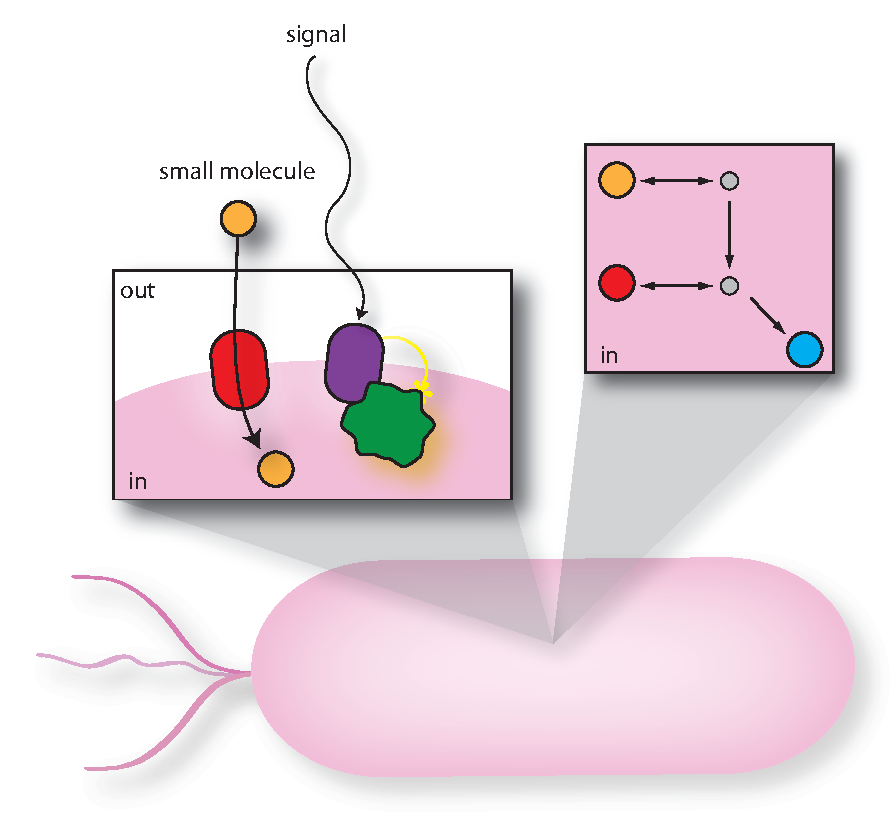
\includegraphics[width=0.6\textwidth]{figures/cell_env_signal_external}
    \caption[Microbes live in changing environments]{Microbes live in changing environments. Both internal and external environments constantly change. Cells sense and respond to changes in the external environment, in part, by transport and signaling. Internal cellular conditions can also be sensed. The right inset depicts several chemical transformation processes that constitute metabolism. Flux through these pathways can be monitored and adjusted by mechanisms described in Figure \ref{fig:chap1:cellrelay}.}
    \label{fig:chap1:cellsense}
\end{figure}

While the genome is mostly static with respect to the lifetime of a single individual, expression of gene products from it is dynamic. This allows the cell to adjust its physiology to changing circumstances. Depending on the environment, microbes vary which genes and pathways are expressed, tailoring their physiology to increase fitness. This process of physiological adjustment relies on sensing information about the internal or external environment, relaying that information within the cell, and ultimately responding by controlling which combination of genes are produced.   

\begin{figure}[h!]
    \centering
    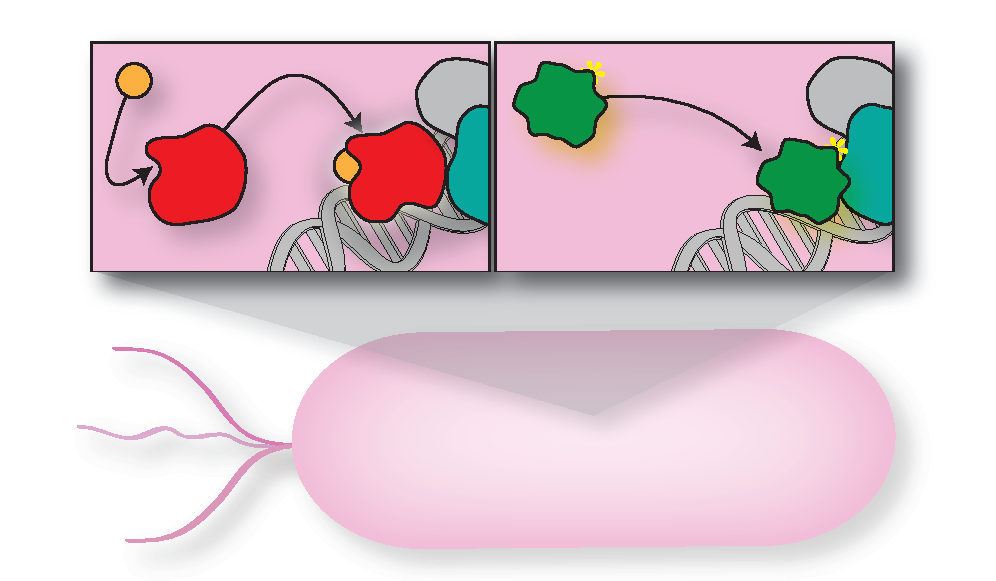
\includegraphics[width=0.6\textwidth]{figures/cell_env_internall}
 	\caption[Cells relay information to regulate the genome]{Cells relay information to regulate the genome. Continuation of Figure \ref{fig:chap1:cellsense}. Regulatory proteins called transcription factors (TFs) control expression at gene promoters. TFs contain DNA binding domains that allow them to recognize and bind to specific nucleotide sequences. In response to binding, these factors can either facilitate or inhibit recruitment of the RNA polymerase to initiate transcription. TFs can be activated by binding/unbinding of small molecules (i.e., allosteric activation/inhibition) or other post-translational modifications (e.g., phosphorylation in eukaryotes). When TFs are activated/inactivated TFs bind to/release from DNA to control the process of transcription at that location.}
    \label{fig:chap1:cellrelay}
\end{figure}

\subsection{Model organisms to study gene regulatory systems}

Many organisms have been developed to study regulation, ranging in scale and complexity from prokaryotic to mammalian systems. Notable examples of organisms used for genome-wide modeling and experimental characterizations include \textit{S. cerevisiae} \cite{schwikowski_network_2000, segal_module_2003}, \textit{B. subtilis} \cite{oh_genome-scale_2007}, \textit{E. coli} \cite{huerta_regulondb:_1998}, \textit{H. salinarum} \cite{bonneau_predictive_2007}, and \textit{M. genitalium} \cite{karr_whole-cell_2012}. In this project, we utilized two of these organisms, \textit{E. coli} and \textit{H. salinarum}. The motivation for selection of each is described below.

\paragraph{\textit{Halobacterium salinarum sp. NRC-1}} is a halophilic archeon. Several biological features make it an interesting organism to study: (1) \textit{Halobacterium} has evolved to thrive in environmental conditions that would be lethal to most species, including exposure to extreme salinity (up to 5.2M NaCl), frequent desiccation-rehydration cycles, high doses of UV radiation, and regular influxes of transition metals and other environmental contaminants. (2) transcriptional regulation in \textit{Halobacterium} is a hybrid of eukaryotic and prokaryotic mechanisms. The general transcription factors (GTFs) comprise multiple orthologs of two eukaryotic GTFs: TFIIBs (TFB) and TATA binding proteins (TBPs). There are 42 possible TFB-TBP pairs, each of which may uniquely regulate expression in different conditions and contribute to niche adaptation \cite{facciotti_general_2007,turkarslan_niche_2011}. Finally, (3) \textit{Halobacterium} possesses functional capabilities that make it a candidate for biotechnology applications. For example, the light-driven proton pump bacteriorhodopsin, which is normally used as an alternative energy source under low oxygen tension, has received interest as an element in optoelectronic devices and photochemical processes \cite{oren_industrial_2010}.  \textit{Halobacterium} is an attractive gene regulatory model system because it contains a relatively small, fully sequenced and annotated genome (2.6 Mbp, ~2400 genes) consisting of one large circular chromosome and two smaller plasmids (pNRC100 and pNRC200). In addition, \textit{H. salinarum} is easy to culture and manipulate genetically, making it useful for laboratory experiments. For the purposes of modeling, it is attractive because of the large amount of data and relatively little knowledge about the genetic underpinnings of its physiology, which make it ideal for model-derived biological discovery. There are currently 1,495 transcriptome profiles available for \halo\ (see \ref{halodata} for additional details)

\paragraph{\textit{Escherichia coli K12 MG1655}} is a gram-negative, facultatively anaerobic, gammaproteobacteria. Apart from human health concerns of pathogenic strains of \textit{E. coli}, the bacteria has been used extensively in biotechnology and investigation of basic biological mechanisms since the foundational work of Lederberg and Tatum on bacterial conjugation in the 1940s \cite{tatum_gene_1947}. \textit{E. coli} has been subject to a wide-array of high-throughput experiments to characterize its genome \cite{blattner_complete_1997}, transcriptome \cite{tjaden_transcriptome_2002}, proteome \cite{taniguchi_quantifying_2010}, and even fitness landscape \cite{nichols_phenotypic_2011}. Large gene expression compendiums exist for the organism. Several computational approaches to reverse-engineer gene regulatory networks directly from gene expression data have used these public \textit{E. coli} data sets \cite{lemmens_distiller:_2009,michoel_comparative_2009,de_smet_ensemble_2011,mordelet_sirene:_2008}, including an organized world-wide competition \cite{marbach_wisdom_2012}. There are currently 868 transcriptome profiles available for \eco\ (see \ref{ecodata} for additional details)

\subsection{Prokaryotic gene regulatory mechanisms}

Prokaryotes regulate expression of their genomes at several stages of production using multiple strategies and mechanisms. Generation of a protein product from a genetic locus can be regulated by controlling DNA structure and accessibility, transcription initiation, transcription elongation, or transcription termination; bacterial mRNAs can even be regulated post-transcriptionally through the action of small RNAs (sRNAs) This project focused on transcription initiation. 

Assembly of RNA polymerase (RNAP) at gene start sites is a critical first step for transcription. In bacteria (like \textit{E. coli}), RNAP first binds to one of the $\sigma$ specificity factors, like the housekeeping $\sigma^{70}$ factor. This holoenzyme complex can then recognize and bind to specific sequences at -35 and -10 nt upstream of gene start sites. In archaea (like \textit{H. salinarum}), the mechanism is more complicated. The archaeal RNAP resembles the eukaryotic RNA polymerase II machinery, where TBP and TFIIB (two general transcription factors) assist the RNA polymerase in locating gene start sites. \textit{H. salinarum} encodes six \textit{tbp} and seven \textit{tfb} genes \cite{baliga_is_2000}. Regulation involving different combinations TBPs and TFIIBs has been shown to facilitate large-scale physiological changes \cite{facciotti_general_2007} and niche adaptation \cite{turkarslan_niche_2011}. 

Additional DNA regulatory proteins, called transcription factors (TFs), facilitate (activators) or prevent (inhibitors) recruitment of RNAP to gene start sites. TFs also recognize sequence specific sites in gene promoters. Many gene promoters contain binding sites for more than one TFs, in addition to the basal $\sigma$ (or TFIIB/TBP) sites. A majority of regulatory sites occur with -250 nt to +50 nt of the gene start site in prokaryotes. TFs themselves can be categorized into two primary types: global and specific. As their name implies, global regulators regulate many genes (on the order of hundreds to thousands in prokaryotes). Typically these factors sense broad environmental shifts, like nutrient changes (e.g., CAP) or anaerobic conditions (e.g., FNR), or starvation and stationary phase (e.g., $\sigma^{38}$). Specific regulators control fewer genes, often targeting genes involved in a specific biological processes or pathway (e.g., LacI, inhibitor of lactose catabolism genes). Coordination microbial genomes results from combinations of interactions between specific and global regulators. 

\subsection{Discovery of regulatory interactions}

An early goal of systems biology was to map the physical interactions between every TF and DNA. Such a physical interaction map would represent a complete gene regulatory network (GRN), which is described in detail below. A number of methods have been developed to identify TF $\rightarrow$ gene interactions, including \textit{in vivo} methods like ChIP-chip \cite{blat_cohesins_1999} (now largely replaced by ChIP-seq, which has finer resolution \cite{johnson_genome-wide_2007}), yeast two-hybrid \cite{fields_novel_1989}, and DNase I hypersensitivity \cite{crawford_identifying_2004}, as well as \textit{in vitro} methods like systematic evolution of ligand by exponential enrichment (SELEX) \cite{blackwell_differences_1990}. Each can be used to elucidate binding sequence preferences of TFs and/or report locations throughout the genome that are physically bound by a particular TF. For those methods that report segments of the genome bound by a TF, each differs in its resolution, false positive rate, and extent to which it is a chimera (e.g., TFs for ChIP-chip are modified with functional groups for biochemical isolation),leading to contention about the trustworthiness of each approach. Knowledge generated from each of these methods, however, is limited to conditions in which the experiments were performed. Rather than providing a complete, unbiased map of TF binding locations, these approaches provide a snapshot of where TFs are bound in a particular condition. 

\subsubsection{Position-specific scoring matrices (PSSMs) quantify the sequence preference of TFs}

\label{pssms}

TFs recognize DNA by sequence-specific electrostatic interactions and Van der Waals forces between evolutionarily conserved DNA-binding domains (DBDs) and DNA along the major groove. Different families of DBDs have evolved to interact with DNA in different ways. The helix-turn-helix domain, for example, consists of $\sim$20 amino acids that use hydrogen bonding to bind two $\alpha$-helices along the major groove, whereas the leucine zipper domain forms two vertical $\alpha$-helices that act as dimerization domains. Identification of putative TFs and assignment to domain families can be accomplished by locating DBDs in protein coding sequence through alignment. 

A critical challenge for understanding genetic regulation by TFs is to describe what sequences they prefer to bind. This provides information about (1) how specific a TF is for DNA, and (2) where in the genome a TF may bind. Discovery of TF binding sequence preference is accomplished by alignment. Given a list of sequences putatively bound by a TF, those sequences can be aligned and a motif constructed by counting up the frequency of nucleotides at each position and scaling by its information content (Figure \ref{fig:chap1:pssm}). These putative bound sequences can originate from observed binding (e.g., ChIP-seq) or computational identification (e.g., \cm\, see \ref{chap:2:cmonkey}) There are several well-established computational algorithms for motif discovery (e.g. MEME/MAST \cite{bailey_fitting_1994,bailey_methods_1998}), as well as searchable databases for known motifs (e.g. STAMP \cite{mahony_stamp:_2007}). 

\begin{figure}[h!]
    \centering
    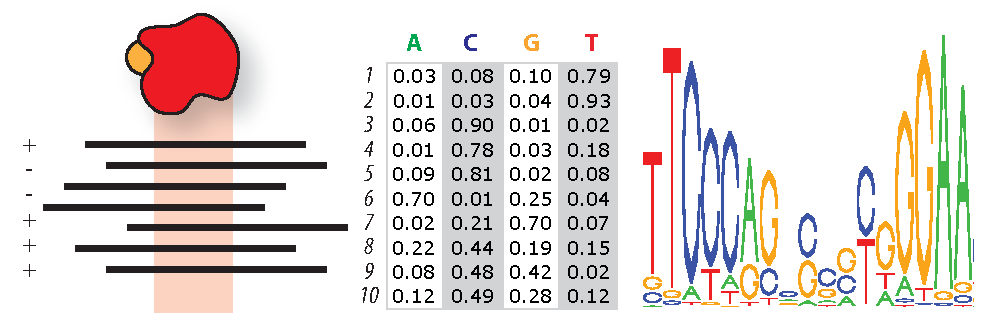
\includegraphics[width=0.9\textwidth]{figures/pssm}
 	\caption[Position specific scoring matrix (PSSM) and motif logo]{
 	Binding sequence preferences for TFs are described by a position specific scoring matrix (PSSM) or position weight matrix (PWM). After aligning sequences putatively bound by a TF (left), the identity of each nucleotide is counted at each position to generate a relative frequency (center; PSSM or PWM). These frequencies are scaled by information content at each position for viewing as a motif logo. An example motif logo is shown at right. 
}
    \label{fig:chap1:pssm}
\end{figure}

\subsection{Canonical genetic control modules}

Grouping coordinated elements of biological systems into discrete modules is critical to understand their operation and evolution. Regulatory proteins, for instance, consist of multiple domains (like DNA binding domains), each with a particular structure and function. These domains include multiple amino acids that are found in similar configurations across many proteins to confer a similar activity. Likewise, single genes rarely explain the behavior (or malfunction) of biological systems. Rather, many genes act in concert to perform a particular task. We refer to discrete units of biological organization as modules. While the idea of modularity is intuitive, defining these modules turns out to be quite challenging, especially from data. 

\subsubsection{Modularity in Biology}

The latter part of the $20^{th}$ century witnessed an explosion of scientific knowledge. Beyond genomes, countless other -omes were generated. From transcriptomes to proteomes, and even phenomes. Although such high-throughput cataloging is still commonplace, efforts to deduce how these molecular parts function together - when, why, and how - are now more widespread. Such efforts are at the heart of the nascent field of systems biology. Hartwell \textit{et al.} wrote a perspective in 1999 \cite{hartwell_molecular_1999} that anticipated an ongoing paradigm shift in biology. The authors argued that investigating molecular biology from the perspective of single genes or proteins, or even across a single molecular type would be insufficient to understand the complex organization and function of biological systems. Instead, they  stressed a need for understanding how the molecular parts interact to form modules and how those modules interact to generate higher-order features.

Understanding biological systems at a genome-scale requires new tools, conceptual frameworks, and language. A first step in this process is to organize and abstract the components into modules. From the perspective of genetic regulation, modules consist of groups of genes that are either co-expressed or co-regulated. Even microbes contain thousands of genes. \textit{E. coli}, for example, encodes 4,497 genes; the genome of \textit{H. salinarum} contains nearly 2,400 genes. Deciphering how these genes partition into modules is non-trivial task. Furthermore, the boundaries defining modules are fuzzy. After all, co-expression in \textit{some} environments does not imply co-expression in \textit{all} environments.

Since the foundational work of Jacob and Monod in the 1960's, several definitions of regulatory modularity have emerged. In the following sections I define each. The following organizational paradigms attempt to group multiple genes into functional units or modules. The definitions vary in terms of the size of modules generated and with respect to assumptions regarding their basic purpose. It is important to remember that no single definition is correct; rather, each is a contrasting lens through which we can understand coordination of genetic expression.   

\subsubsection{Operon}

The original co-regulatory module described by Jacob and Monod \cite{jacob_genetic_1961} is also the most simple. The \textit{operon} simply consists of multiple, adjacent genes that are transcribed as a single, polycistronic transcript. There are many operons in bacterial genomes. \textit{E. coli}, for example, encodes nearly 700 operons \cite{salgado_operons_2000}. Nearly half of the genes in the \textit{E. coli} genome are in operons.  Operons, however, should not be considered dogmatically. Many operons express condition-specific isoforms. While genes of an operon may be co-transcribed in some condition, many contain internal binding and termination sites that result in production of alternative transcripts in some environments \cite{koide_prevalence_2009}. 

\begin{figure}[h!]
    \centering
    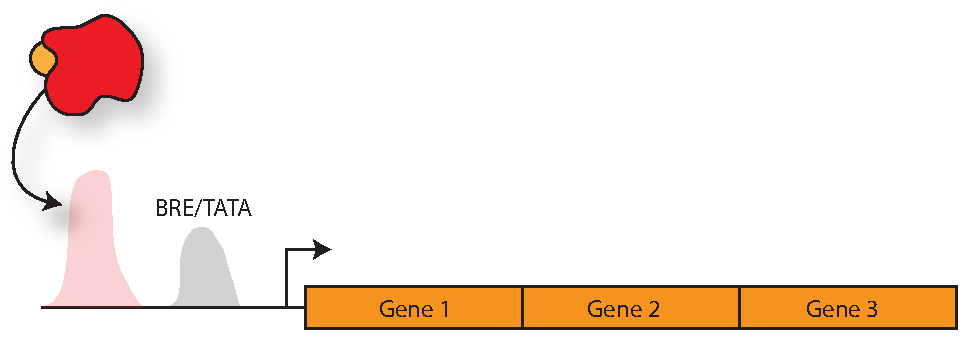
\includegraphics[width=0.9\textwidth]{figures/operon}
 	\caption[Operons: multiple genes transcribed as a single polycistronic transcript]{
 	Operons are co-regulatory units wherein multiple genes are transcribed as a single polycistronic transcript. Several genes involved lactose utilization and transport were discovered to be co-transcribed as a single co-regulated unit in 1961 by Jacob and Monod \cite{jacob_genetic_1961}
}
    \label{fig:chap1:operon}
\end{figure}


\subsubsection{Regulon}

The term \textit{regulon} was coined in 1964 to describe regulation of arginine biosynthetic genes by the repressor, ArgR \cite{maas_studies_1964}. Unlike operons, genes regulated by ArgR are located throughout the genome, including multiple operons like the arginine uptake system, \textit{art}, and histidine transport genes, \textit{hisJQMP}. A regulon consists of genes regulated by a single, common TF (like ArgR). Like operons, there are many regulons in prokaryotes - one for every TF. \textit{E. coli} has 83 annotated regulons \cite{novichkov_regprecise_2012}. The number of genes in a regulon depends on the TF. Sizes can range from several genes to many hundreds, including operons. Several databases collate information about regulons in prokaryotes \cite{alm_microbesonline_2005,novichkov_regpredict:_2010,novichkov_regprecise_2012}. Notably, \href{http://regprecise.lbl.gov/RegPrecise/}{RegRecise} uses evolutionary conservation to refine regulon predictions across multiple species \cite{novichkov_regprecise_2012}.

\begin{figure}[h!]
    \centering
    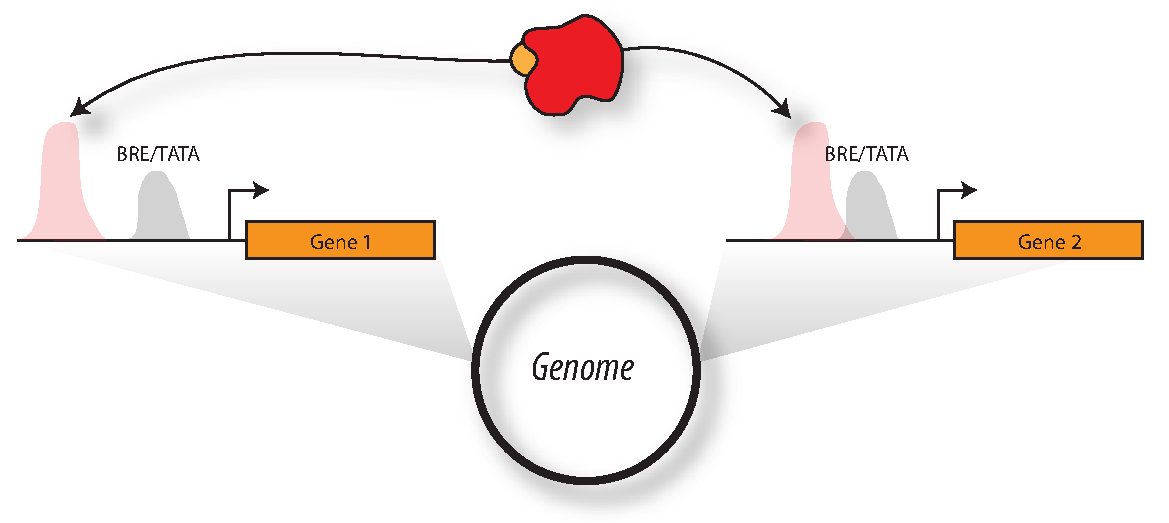
\includegraphics[width=0.9\textwidth]{figures/regulon}
 	\caption[Regulon: multiple gene regulated by a common transcription factor]{
 	A regulon consists of multiple genes or operons located throughout the genome that are co-regulated by a common transcription factor. The ArgR regulon was first described in 1964 by Maas and Clark \cite{maas_studies_1964}.
}
    \label{fig:chap1:regulon}
\end{figure}

\subsubsection{Modulon}

A \textit{modulon} is a collection of operons and regulons that are regulated by a common pleiotropic TF in addition to different specific TFs. Canonical examples include the CAP modulon, a nutrient-responsive modulon that affects the \textit{lac} operon as well as the arabinose catabolism operon (\textit{ara} operon), and the FNR modulon \cite{guest_fnr_1996}, which responds to anaerobiosis. Like regulons, all of the genes of a modulon are regulated by at least one common TF, generally a global regulator (i.e., a TF that regulates many genes, typically on account of its low sequence specificity). 

\subsubsection{Stimulon}

A \textit{stimulon} consists of operons and regulons that are regulated by the same stimulus. Well known examples include the yeast $H_{2}0_{2}$ stimulon \cite{godon_h2o2_1998} and the \textit{B. subtilis} heat shock stimulon \cite{schumann_bacillus_2003}. Stimulons include all of the biological pathways and processes that respond to the same environmental change. As such, they can be large, sometimes including thousands of genes. Stimulon genes can increase as well as decrease in expression.

\subsubsection{Corem}

Co-regulated modules or \textit{corems} are the condition-specific modules discovered by EGRIN 2.0. Unlike other definitions of modular genetic regulation, corems can be regulated by multiple, independent TFs. They can contain subsets of operons and regulons, reflecting condition-specific generation of multiple transcriptional isoforms from an operon. They can include genes from multiple regulons and operons. They range in size from small (3 genes) to large (100s of genes). Corems also vary in how often they are co-expressed, from rare ($<$1/10 of the observations) to common ($>$2/3 of the observations). Importantly, an individual gene can belong to \textit{multiple} corems. A summary of corem statistics for \textit{E. coli} and \textit{H. salinarum} corems is available in Figure \ref{fig:corem_stats}. Defining hallmarks of a corem are depicted in Figure \ref{fig:chap1:corem}. The generation, properties, and utility of corems will be developed throughout the text.

\begin{figure}[h!]
    \centering
    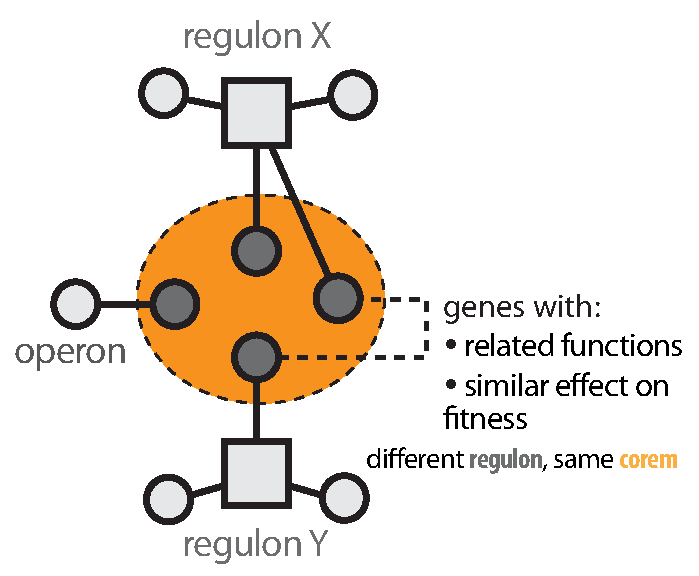
\includegraphics[width=0.6\textwidth]{figures/corem}
 	\caption[Corem: subsets of operons and regulons regulated by multiple transcription factors]{
 	Corems are condition-specific co-regulatory modules discovered by the gene regulatory inference algorithm EGRIN 2.0. Corems can contain subsets of genes from multiple regulons and operons. Each corem has evidence for co-regulation in the form of \textit{cis}-regulatory motifs called gene regulatory elements or GREs. GREs suggest that some corems are regulated by independent factors. Generation and analysis of corems will be described throughout the text. 
}
    \label{fig:chap1:corem}
\end{figure}

\section{Networks in biology}

Networks (or graphs) are mathematical representations of the relationships between objects. Networks consist of nodes (objects) and edges (relationship between the objects). Mathematically, we refer to this entity as a graph, $G = (N,E)$, where the graph, $G$, is an ordered pair comprised of nodes, $N$, and edges, $E$, which themselves are two element subsets of $N$. They can be represented using a (weighted) adjacency matrix, where each entry $N_{i, j}$  indicates a (weighted) relationship between nodes $i$ and $j$.

Networks have become popular to represent biological information, especially from high-throughput screens and experiments. Regulatory influences, protein-protein interaction, and metabolic processes can be represented as networks, where nodes represent regulators, genes, proteins, metabolites or any other biological entity, and edges, which connect nodes, represent arbitrary interactions between the nodes (Figure \ref{fig:chap4:networks}).  A variety of biological networks have been generated, including protein-protein interaction networks \cite{schwikowski_network_2000}, gene regulatory networks  \cite{bonneau_predictive_2007}, metabolic networks  \cite{forster_genome-scale_2003}, even literature citation networks \cite{west_eigenfactor_2010}. Figure \ref{fig:chap4:networks} summarizes important properties of networks. Formalizing biological interactions as networks has a number of analytical advantages. Besides simplifying the representation of biological interactions, graphs have a long, well studied history. Structuring biological relationships in a graph gives access to richly developed tools of graph theory.  Conveniently, many of the mathematical concepts and statistical measures developed for abstract graph structures also apply to biological networks. A graph can be analyzed mathematically to reveal characteristics of its topology. Since the structure of interactions in a network is oftentimes directly related to dynamical properties of that network, topological analysis can give insight into the organization and function of biological systems. Important topological features of biological networks include community structure (e.g., biological modules), hierarchical organization (e.g., nearly power-law degree distributions), and overrepresented network motifs (e.g., the three gene feed-forward loop). These topological features of biological networks and their consequence for the function of biological systems will be explained in more detail throughout the text. 

\begin{figure}[h!]
    \centering
    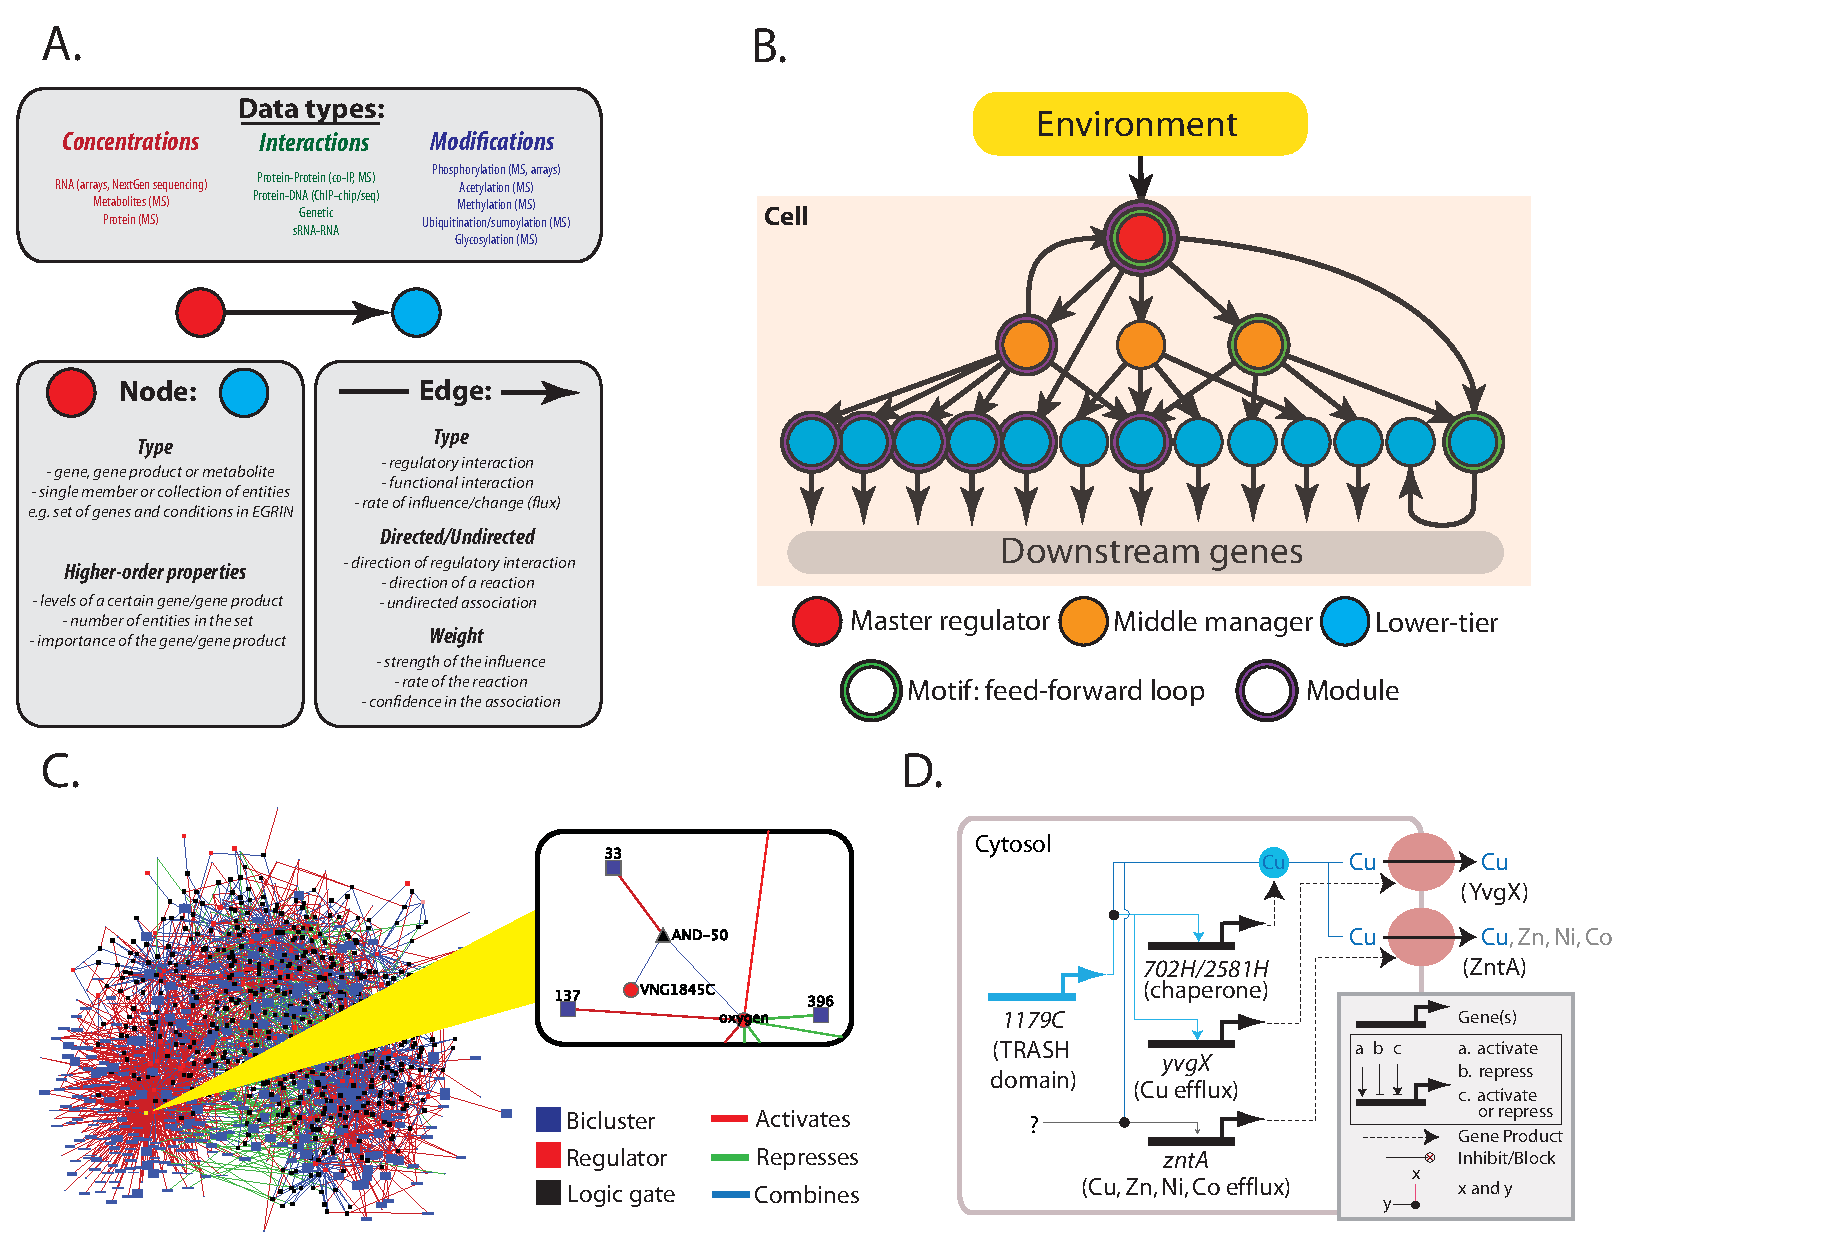
\includegraphics[width=0.9\textwidth]{figures/review_figure1}
 	\caption[Generation and properties of networks]{
 	(A) The fundamental units of a network (or graph) are nodes, and edges. Three types of biological information are commonly represented as a network: transcriptional, metabolic, and protein-protein interactions. (B) Biological networks share common features. (1) hierarchy: transcriptional networks are close to scale-free in the distribution of regulatory connections and exhibit hierarchical arrangement of connections \cite{barabasi_network_2004}. (2) modularity: biological networks aggregate pathways and functions into modules \cite{hartwell_molecular_1999}. Here, we denote a transcriptional “module” by a purple ring surrounding the nodes in the module. (3) motifs: interesting dynamic behaviors of gene circuits are often mediated by particular wiring of the parts, which defines a network motif. The members of a particularly well-studied network motif, the feed-forward loop, are depicted in this illustration by green circles surrounding the nodes \cite{alon_network_2007}. (C) Biological networks learned from experimental data, such as the Environmental and Gene Regulatory Influence Network (EGRIN) for \textit{H. salinarum sp. NRC-1}, contain many layers of information that can be mined to aid hypothesis generation \cite{bonneau_predictive_2007}.
}
    \label{fig:chap4:networks}
\end{figure}

\subsection{Gene regulatory networks (GRNs)}

Regulatory interactions can be cataloged, visualized, and analyzed as gene regulatory networks (GRNs). GRNs can encode who regulates whom, when, where, and to what extent. Analysis of GRNs has revealed valuable insight into how cells process information \cite{barabasi_network_2004} and control expression of their genomes. 

GRN sub-networks that respond to environmental change range from simple to complex. In the simplest case, two-component relay systems directly couple environmental sensing to gene regulation through activation of a TF (e.g., osmoregulation by EnvZ/OmpR two-component system in \textit{E. coli} \cite{aiba_evidence_1989}). Most natural environments, however, change in more complicated ways. Microbes must decipher  many overlapping signals, some of which are prone to high levels of noise. To make the task even more complicated, genetic circuits are not isolated from one another. Even simple relay systems exhibit cross-regulation with other regulatory circuits and can affect other cellular components indirectly \cite{laub_specificity_2007}. To achieve robust response to complicated environmental signals, cells have evolved mechanisms to handle errors, cross-talk, and noise. This accomplished, in part, by encoding gene regulation in combinatorial, modular regulatory circuits that confer robustness to the system.   

\subsection{Discovery and Inference of GRNs}

Obtaining accurate information about regulatory interactions is critical to draw conclusions about biological function from network structure. Considerable effort over the past decade has been dedicated to obtaining accurate GRNs. These efforts fall into two major categories: experimental and computational approaches. The two are not mutually exclusive; in fact, computational approaches always build from experimental observations. The two approaches do, however, vary in the amount of time and money required to obtain comprehensive and accurate GRNs. 

\subsubsection{Experimental Approaches}

Experimental data is the starting point for all GRN reconstruction. An annotated genome is a minimum requirement. The units of the GRN - in this case genes - must be defined. Regulatory proteins (TFs) must also be defined. For newly sequenced genomes, this is accomplished by searching within the new genome for DNA binding domain (DBD) homologies (described above, \ref{pssms}) \cite{bonneau_comprehensive_2004}. Those genes with DBDs are considered putative TFs. 

After basic genome annotation, several approaches for GRN reconstruction exist. The most obvious involves direct measurement of TF binding events across the genome using ChIP-chip or ChIP-seq. Each binding event in the promoter region of a gene (observed after filtering at some confidence threshold) can be considered an edge between a TF and gene in the GRN. Other experimental methods, like \textit{in vitro} binding of purified TF to a promoter  sequence can be used to support the assignment. While attractive, such approaches suffer from two complications: (1) they require separate experiments for each TF. This, in turn, requires developing a purification strategy for each TF, typically using genetic modification (e.g., HA-tag). For bacterial genomes, this would require at least 100 separate strains and experiments for a complete GRN. (2) More troubling, is that observed TF$\rightarrow$gene binding is condition-specific. This means that experimentally-based GRNs only reflect the conditions in which the data were collected. For interaction-based assays (like ChIP-chip or ChIP-seq) to be comprehensive, they would need to be measured in many conditions. Designing experiments to test all pairs of TF and relevant conditions would lead to combinatorial explosion. New technologies like DNase I hypersensitivity \cite{crawford_identifying_2004} promise to overcome some of these challenges by measuring all bound sites throughout the genome in a single experiment. Currently, however, it is difficult to resolve which TF is bound to a particular fragment without \textit{a priori} knowledge of the binding preferences of TFs. Other challenges exist for using these methods in bacterial genomes. 

Several resources have been developed to share experimental knowledge of GRNs across laboratories. RegulonDB, for example, is a database of all evidence for transcriptional regulation collated for \textit{E. coli} \cite{salgado_regulondb_2006}. The collection of data in RegulonDB represents over 50 years of experimental work to characterize the GRN from a single organism. This highlights how challenging it is to reconstruct GRNs directly from experimental data. In the absence of technological innovation, GRN reconstruction in newly sequenced species through experimental approaches alone will be time and cost prohibitive. Many investigators, therefore, have considered alternative approaches to rapidly infer GRNs, especially for understudied organisms. Usually these alternatives employ computational inference methods. 

\subsubsection{Computational Approaches}

Computational approaches attempt to reverse engineer GRNs directly from experimental data. While such methods are always underpowered (i.e., there are too few observations for the number of variables in the system), computational inference methods have made significant improvements, greatly increasing predictive accuracy. One of the biggest gains for these methods came from including biological priors (i.e., using biological knowledge to assist inference). Especially in understudied organisms, computational inference is the only viable alternative to costly, brute force experimentation for GRN reconstruction. 

The primary source of data used for most computational approaches is gene expression. Microarray and RNA-seq allow for quantitation (absolute or relative) of every gene in the genome with a single experiment. To deduce a GRN from these measurements, inference algorithms universally assume that these expression patterns result from some reproducible genetic ``program''. The aim of computational methods is to use data to figure out the program. From this perspective, biological inference is also a problem of pattern recognition (constrained by biological mechanism). Given a sufficient number of observed expression profiles (e.g., different experimental conditions), one can deduce an underlying network that produced them (at least one of many networks that is consistent with the data). The promise of these approaches is that gene expression data is relatively easy and cheap to collect, even in understudied organisms. 

 Full description of computational methods used to infer gene regulatory networks will be provided in Chapter \ref{chap:2} It should be noted that GRN inference methods vary substantially: from correlation to causal, and from statistical to information-based. De Smet \textit{et al.} provide a comprehensive review of GRN inference methods, highlighting the advantages and shortcomings of each \cite{de_smet_advantages_2010}. 

\section{Systems-level view of gene regulatory organization}

 GRN analysis reveals valuable insight into how cells process information. A systems perspective is essential for deciphering how microbes coordinated expression of their genomes. Just as genes work in concert to mediate environmental responses, multiple TFs work together to coordinate the dynamic activity of GRNs. GRNs are impossible to characterize from the perspective of a single TF. 

 Early topological investigations of GRNs revealed several insights. First, not all regulators are equivalent; few transcription factors (TFs) regulate many genes, whereas the majority of TFs regulate far fewer downstream genes (Reviewed in \cite{barabasi_network_2004}). Second, GRNs are hierarchical. ``Master regulator'' TFs, for example, initiate regulatory cascades. While a ``master regulator'' many only interact with few TFs, it can initiate a regulatory cascade by influencing activities of ``middle managers'' that propagate its signal to ``lower tier'' regulators, directly controlling specific processes  \cite{yu_genomic_2006}. Third, some patterns of interactions are statistically overrepresented in biological networks -- these overrepresented subgraphs are called motifs (\cite{milo_network_2002}, Reviewed in \cite{alon_network_2007}). Below I elaborate on the dynamical properties of these features. Finally, abstract representations of gene regulation can yield meaningful dynamic insight into biological processes. Examining the cell-cycle regulatory network as a Boolean representation, for example, reveals the existence of biological attractor states that contribute to the robustness of the cell cycle \cite{li_yeast_2004}.    

As mentioned previously, interpretation of GRNs depends critically on their accuracy. Without correct annotation of TF$\rightarrow$gene relationships, it is impossible to know which TF-gene pairs, for example, are in feed forward loops or which TFs are ``master regulators''.  Network topology is critical to understand network dynamics. In the following sections, I consider the dynamical properties of GRN topological features. 

\subsection{Network Motifs}

Network motifs are frequently appearing topological relationships in directed GRNs. By cataloging frequencies of three gene motifs in \textit{E. coli}, Uri Alon and his colleagues discovered over representation of certain types of motifs in natural GRNs, including feedforward and feedback architectures \cite{milo_network_2002}. These regulatory motifs possess interesting dynamic behaviors, which help cells adjust to changes in their environment. Feedforward loops, for example, buffer noise in highly deterministic biological processes, such as in development \cite{mangan_structure_2003,levine_gene_2005}, while feedback loops provide local sensing and specific response to chemical changes, such as product inhibition exerted in metabolic pathways \cite{neidhardt_escherichia_1996}. Figure \ref{fig:chap1:ffl} provides a graphical representation of the dynamic properties of the feedforward loop. While complete enumeration of all possible three gene architectures made the study by Alon and colleagues possible \cite{milo_network_2002}, there are likely important higher-order motifs in biological systems as well, including global motifs consisting of many component sub-motifs (i.e., motifs of motifs, etc), that may be difficult to assess statistically because of exponential increase in possible topological permutations.

\begin{figure}[h!]
    \centering
    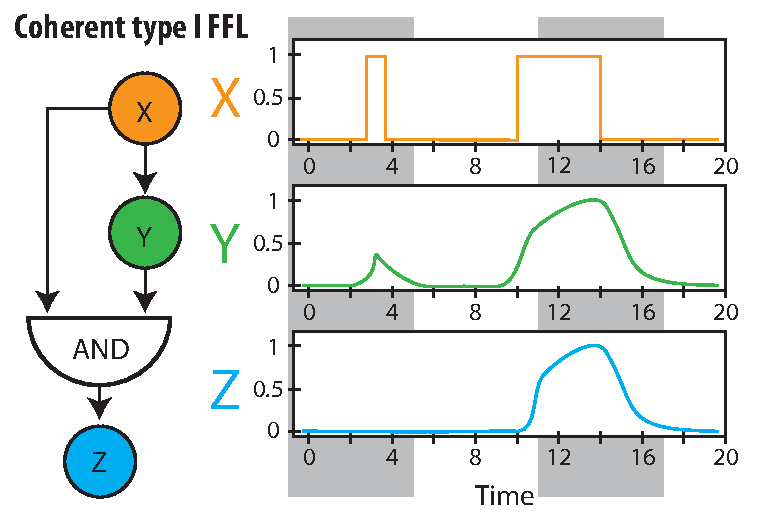
\includegraphics[width=0.7\textwidth]{figures/ffl}
    \caption[Network motifs: the coherent feed-forward loop]{
    The coherent feed-forward motif is a well studied network motif that occurs commonly in biological networks. Like other network motifs, the arrangement of genes into a coherent feed-forward loop has interesting dynamical properties. Feed-forward loops have been shown to buffer noise in biological systems, as well as confer rapid response once a critical signal threshold is reached \cite{mangan_structure_2003}. The cartoon representation depicts downstream expression of $Z$ in response to either a transient or sustained pulse of $X$ (adapted from \cite{mangan_structure_2003}).
}
    \label{fig:chap1:ffl}
\end{figure}

\subsection{Regulatory Logic}

The complete set of TF$\rightarrow$gene interactions in the cell composes a complex regulatory network. This network sets upper and lower bounds on possible expression levels for genes. Dynamic execution of the network leads to coordinated expression of the genome that has evolved to match the sensed environment. Interaction topologies that make up GRNs range in complexity from simple single input motifs (e.g., SIM), to more complicated three gene motifs (e.g., feed forward loop, above), to higher-order architectures involving multiple genes and composed of multiple three-gene (and larger) component motifs (e.g., integrated feedforward loop). These interactions can even compute logic functions, like \textit{and}/\textit{or} gates. Figure \ref{fig:chap1:regLogic} highlights the range of complexity in regulatory logic.

From the standpoint of systems biology, this topological framework helps us understand which genes and functional processes are coordinated in which environments. Observationally, the output of these complex regulatory circuits are co-expression patterns observed in gene expression data. The goal of this project was to group these co-expression patterns into biologically meaningful modules, determine what TFs and regulatory logics were responsible for their generation, and to understand when and why they are co-expressed.  

\begin{figure}[h!]
    \centering
    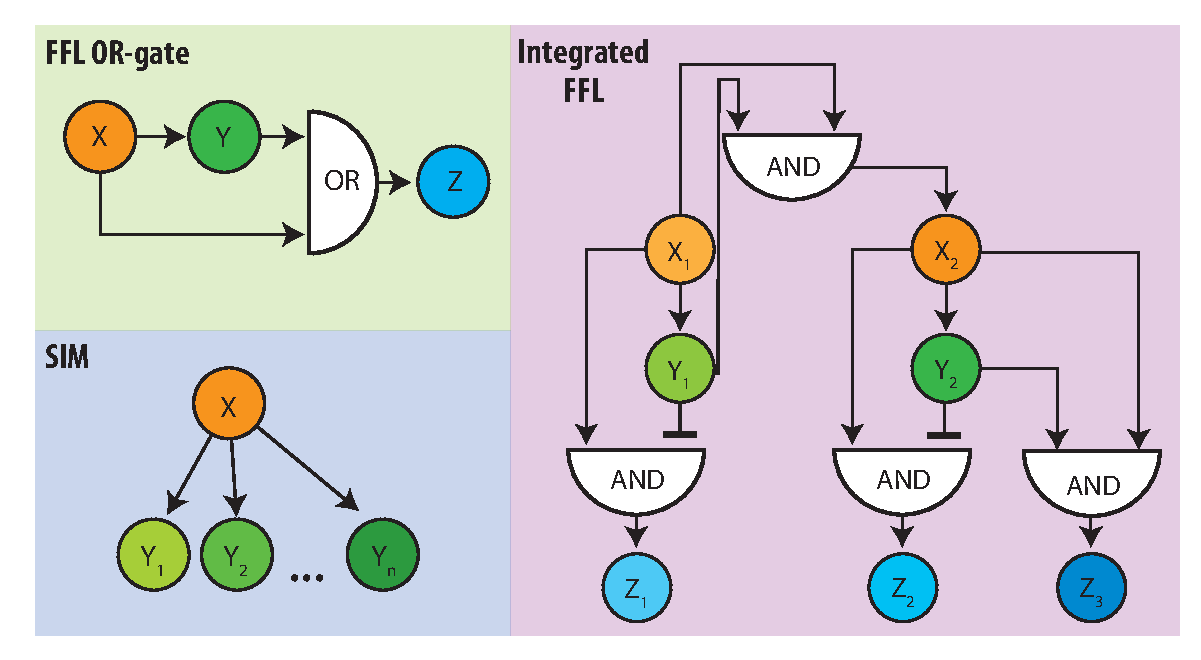
\includegraphics[width=0.9\textwidth]{figures/regLogic}
 	\caption[Varieties of regulatory logic, from simple to complex]{Gene regulatory logic ranges from simple to complex. Three gene regulatory circuits highlight varying degrees of complexity. Note the use of logic gates using \textit{and}/\textit{or} gates. Ultimately, all regulatory sub-circuits (even the simple SIM) are embedded in much more complicated regulatory networks.  
}
    \label{fig:chap1:regLogic}
\end{figure}

\subsection{Beyond the operon and regulon}

In the 1996 edition of \textit{EcoSal}, Neidhardt and Savageau wrote a chapter about regulation of multigene systems entitled, ``Regulation Beyond the Operon'' \cite{neidhardt_escherichia_1996}. The chapter explored concepts of gene expression beyond simple co-linear arrangement of genes in an operon, starting with the regulon and moving to more complex relationships described by modulons and stimulons (described above). While it was clear from the data that genes were co-expressed in complex, condition-specific arrangements, it has been less clear how these patterns emerge from GRN activity. Unresolved questions included: Do genes have to be regulated by a common factor to be consistently co-expressed across environments? What is the role of combinatorial regulation in prokaryotes? Are genes regulated by a common factor always co-expressed? This project attempts to quantify the relationship between gene regulatory modules, GRNs, and the nuanced condition-specific associations between TFs and genes that generate condition-specific co-regulatory modules - directly from data. 

\section{Chapter Organization}

The following chapters investigate the organization, function, and evolution of GRNs in prokaryotes. I develop a comprehensive view of data-driven GRN inference, from model construction (Chapter \ref{chap:2}) to interpretation (Chapter \ref{chap:3}) and implications (Chapter \ref{chap:5}). I explore how the structure and function of GRNs contributes to our understanding of how these networks evolve (Chapter \ref{chap:4}) . 

Chapter \ref{chap:2} discusses computational methods for gene regulatory network inference from genome sequence and large gene expression compendiums. It also describes construction of \egrine, the network ensemble elaborated throughout the text. In addition to complete description of the algorithm, many additional details are documented, including experimental data sets used, benchmarks employed to evaluate model performance, and web-framework developed to facilitate exploration of the model's predictions. Chapter \ref{chap:3} focuses on biological interpretation of \egrine. In particular, it documents the model-assisted discovery of \textit{corems}, condition-specific co-regulatory modules that influence cellular fitness. \ref{chap:4} shifts focus to the evolution of GRNs. I consider how dynamics of environmental change shapes the way GRNs evolve. Finally, \ref{chap:5} investigates the consequences and suggests directions forward, both for improving GRN inference and in context of evolution. 


 

 
 
    % ========== Chapter 2
 
\chapter {\uppercase{Computational approaches to reconstruct gene regulatory networks}}
\label{chap:2}

 A challenge of systems biology has been inference of comprehensive and accurate gene regulatory networks (GRNs) directly from genome sequence and transcriptome data. In this chapter, I describe computational approaches for reverse engineering accurate GRNs from gene expression data. There are diverse approaches to the problem: from information theoretic to correlational to integrated. I focus on two algorithms that play a central role in the work described here: \cm\ \cite{reiss_integrated_2006} and \nwinf\ \cite{bonneau_inferelator:_2006}, as well as the model derived from integrating the two, the Environment and Gene Regulatory Influence Network or EGRIN \cite{bonneau_predictive_2007}. Following introduction of these components, I discuss methods developed specifically for this dissertation, an ensemble of EGRIN models. I review the history and motivation for ensemble modeling. I document all of the methods, data, and analyses used to construct models for \halo and \eco. Additionally, I provide validation for the model's predictions, as well as evaluation of its robustness. The details described in this chapter are the foundation from which I derive biological insight in the following chapters.\\

 \noindent This chapter has been modified from the supplement to: \\

 \noindent Brooks AN$^{*}$, Reiss DJ$^{*}$, Allard A, Wu W, Salvanha DM, Plaisier CL, Chandrasekaran S, Pan M, Kaur A, Baliga NS. (2014) A system-level model for the microbial regulatory genome. \emph{Mol Syst Biol.}  10: 740.\\

 \noindent * Indicates equal contribution 

 \paragraph{Chapter Highlights}

	\begin{itemize}
	\item Many algorithms for GRN inference exist. Methods vary significantly in their approach. 
	\item \cm\ integrates multiple sources of biological data, including gene expression, to identify condition-specific co-regulatory modules called biclusters
	\item \nwinf\ predicts which TFs influence condition-specific regulation of these biclusters using regression and variable selection
	\item Together, the two algorithms generate an Environment and Gene Regulatory Influence Network (EGRIN)
	\item Ensemble network inference in \egrine\ improves performance by reducing model variance and allowing detection of rare co-regulatory events 
	\item We derived biological insight from the ensemble model by applying network-based methods for backbone extraction and link community detection
	\item Extensive support for model predictions from independent experimental validation data
	\item \egrine~outperforms other GRN inference methods 
	\end{itemize}

\section{Summary}

Many methods exist for reconstructing GRNs from transcriptomic data. Integrating additional supporting data can assist network reconstruction. \cm\ is a stochastic semi-supervised machine learning algorithm for inferring GRNs that uses \textit{cis}-regulatory motif detection and biological support in known functional networks to constrain model selection. \nwinf~predicts influence of TFs on the expression of \cm~biclusters. Running \cm\ and \nwinf~in an ensemble framework greatly improves performance. The resulting \egrine\ model is more accurate and reveals genetic mechanisms through which bacteria reuse gene modules across diverse environments to enhance fitness.  

\section{Existing computational approaches}

There are many approaches to GRN inference. So many, in fact, that entire reviews have been written about them \cite{bansal_how_2007,de_smet_advantages_2010}. There has even been a formal competition between algorithms. While full description of all approaches is outside the scope of this manuscript, I briefly cover some of the more popular methods, especially those that factor into the present study. 

Methods for GRN inference vary significantly in their fundamental approach to the problem. While each tries to infer an accurate and comprehensive GRN directly from gene expression data, many of the methods take fundamentally different approaches. Some methods use regression (e.g., \nwinf\ described extensively below), some correlation (e.g. WGCNA); some are information based (e.g., CLR and ARACNE), whereas others are Bayesian; others still are integrated, using additional data to perform inference (e.g., \cm) or use other methods entirely (e.g. Genie3 \cite{huynh-thu_inferring_2010}).Newer methods, including our own and DREAM5, aggregate across multiple runs of the same algorithm (e.g. \egrine, the method developed here) or integrate across multiple, heterogeneous methods (e.g, DREAM5).

\paragraph{CLR} Context likelihood of relatedness, CLR \cite{faith_large-scale_2007}, is a mutual information based approach that builds on relevance networks \cite{eisen_cluster_1998,butte_mutual_2000}. CLR (like relevance networks) calculates mutual information between each TF and every gene in the genome using mutual information (MI), where mutual information is a measure of the statistical dependence between two variables. The resulting network can be cut at some threshold MI value to produce a GRN (only TF$\rightarrow$gene above the threshold are retained). CLR adds to relevance networks by introducing an adaptive background correction step that tries to assess how significant each TF$\rightarrow$gene MI value is in the context of every other possible interaction for either that TF or gene. Only those that MI values that are statistically distinguishable from background are retained.  This step is designed to remove indirect dependencies in the network to retain only direct TF$\rightarrow$gene interactions. 

\paragraph{ARACNE} ARACNE is also an information theoretic approach to reconstructing GRNs \cite{margolin_aracne:_2006}. It uses MI to infer TF$\rightarrow$gene interactions as well. Unlike CLR, it uses the data processing inequality (DPI) to remove indirect dependencies. DPI removes the lowest MI from every every gene triplet in network above a certain threshold. The basic idea is that direct interactions will have a higher MI. Thus in the following three gene scenario: $A \rightarrow B \rightarrow C$, $MI_{A,C} < MI_{B,C}$.

\paragraph{WGCNA} Weighted gene correlation network analysis, WGCNA, computes pairwise correlation (weighted or unweighted) between every pair of genes followed by hierarchical clustering and dynamic tree cut to define gene co-expression modules \cite{langfelder_wgcna:_2008}. Unlike ARACNE and CLR, WGCNA does not specifically predict TF$\rightarrow$gene interaction, rather it produces gene co-expression modules (like the \cm\ component of EGRIN, described below).

\paragraph{DISTILLER} DISTILLER, like \cm, produces biclusters (sets of gene co-expressed in subsets of the experiments) by integrating gene expression data with interaction data from RegulonDB \cite{lemmens_distiller:_2009}. DISTILLER is one of the algorithms we compare our method against (given their similarities). We obtained \textit{E. coli} expression data from this paper. 

\paragraph{DREAM5} Dialogue for Reverse Engineering Assessments and Methods (DREAM) is an annual competition for computational methods. In 2012, a group running the competition made a community network of all the top scoring entries for a GRN inference challenge. As described below, this is a type of ensemble model (similar in spirit to our own). The group integrated the predictions from various methods using Borda count election method. Basically, they retained the TF$\rightarrow$gene predicted by the most algorithms. 

\paragraph{EGRIN} Environment and Gene Regulatory Influence Network (EGRIN) uses biclustering in addition to regression and variable selection to infer both gene modules (biclusters) and specific TF$\rightarrow$gene influences \cite{bonneau_predictive_2007}. The approach consists of the algorithms \cm\ \cite{reiss_integrated_2006} and \nwinf\ \cite{bonneau_inferelator:_2006}. Since these algorithms are the basis for this dissertation work, they will be described in great detail below. \\

\noindent A comprehensive review of available methods and comparison between them is available in \cite{de_smet_advantages_2010} and the supplement to \cite{marbach_wisdom_2012}.

\subsection{Integrated biclustering using \cm}

\label{chap:2:cmonkey}

\subsubsection{\cm\ introduction}

The \cm\ integrated biclustering algorithm was described and fully benchmarked in \cite{reiss_integrated_2006}. In short, the algorithm computes putatively co-regulated modules of genes over subsets of experimental conditions from gene expression data, constrained by information provided by genome sequence (\textit{de novo} identification of conserved \textit{cis}-regulatory motifs in gene promoters), and functional association networks. Its defining characteristic is that it combines all three types of data (expression, sequence and networks)together into an integrated model that uses a stochastic optimization procedure to identify modules that best satisfy all three constraints, simultaneously.

The \cm\ integrated biclustering algorithm identifies groups of genes co-regulated under subsets of experimental conditions, by integrating various orthogonal pieces of information that support evidence for their co-regulation, and optimizing biclusters such that they are supported by one or more of those additional constraints. The three sources of evidence for co-regulation leveraged by \cm\ to score gene clusters are (1) tight co-expression in subsets of available gene expression measurements (similarity of expression profiles); (2) quality of \textit{de novo} detected \textit{cis}-regulatory motifs in gene promoters (putative co-binding of common regulators); and (3) significant connectivity in functional association or physical interaction networks (co-functionality). The algorithm served as the cornerstone for the construction of the first global, predictive Environmental Gene Regulatory Influence Network (EGRIN) model for \halo\ \cite{bonneau_predictive_2007}, and has now been applied to many additional organisms (\eg, \cite{yoon_systems_2013} and unpublished).

To run \cm\ as part of an ensemble-based inference approach required significant updates to the \cm\ algorithm. These updates primarily addressed computational inefficiencies that led to long runtime. The primary algorithm modification in the new implementation is global optimization (rather than the local, individual cluster optimization utilized by the original procedure). Additional algorithm updates include changes to the individual scoring scheme for subnetwork clustering, as well as integration of the scores. All of these changes improved the procedure's runtime without significantly affecting the algorithm's performance.

\begin{figure}[h!]
\centering
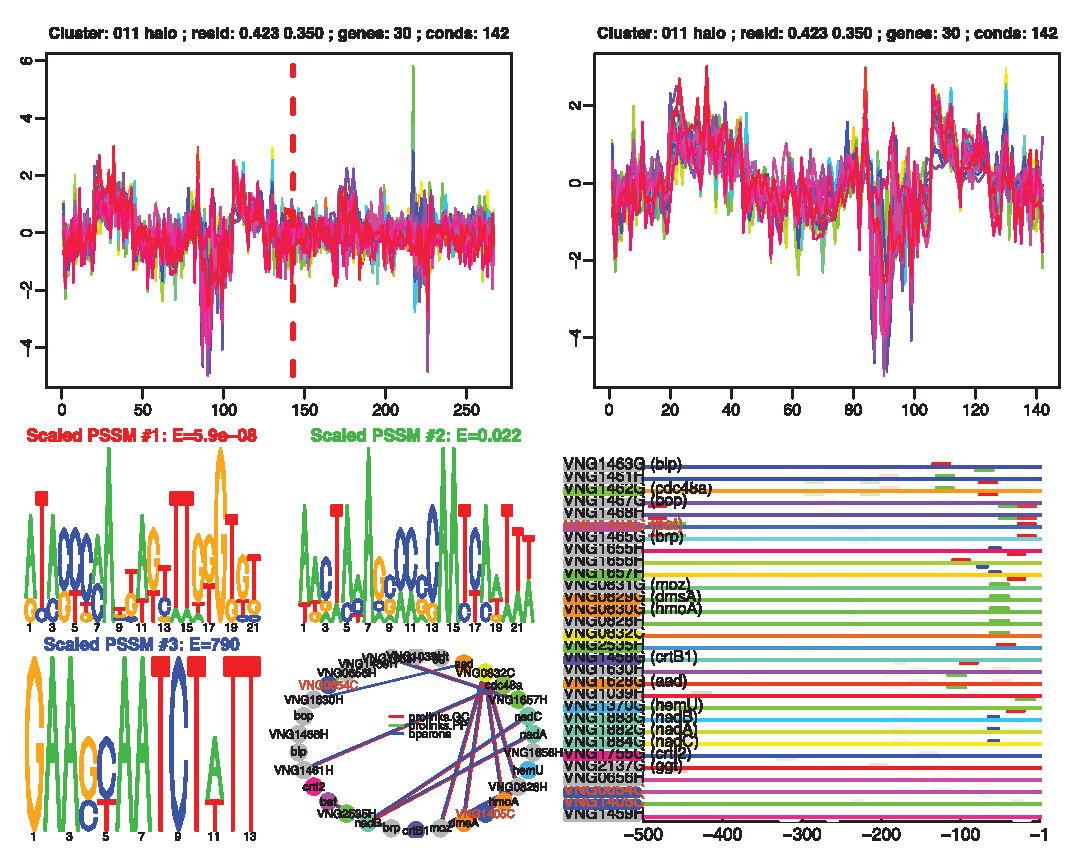
\includegraphics[width=0.9\linewidth]{figures/bicluster}
\caption[Bicluster: a conditionally co-regulated module]{\cm\ produces a set of biclusters ($\sim$300), each of which consists of a group of genes that are co-regulated in some (but not all) of the experiments. Typical \cm\ bicluster is shown here. Top-left: Standardized gene expression values for each gene in the bicluster. Vertical red line separates conditions that have been excluded from the bicluster. Top-right contains an expanded view of only the conditions in which the genes are co-expressed. \cm\ also uses \textit{de novo} motif detection to support bicluster assignment. Upstream regions of bicluster genes are searched for shared \textit{cis}-regulatory motif by MEME \cite{bailey_fitting_1994}. Similarity of the genes in annotated functional networks (e.g. STRING \cite{szklarczyk_string_2011}) is also scored. Detected motif and string network shown at bottom-left. Location of the motif in gene promoters shown bottom-right.}
\label{fig:bicluster}
\end{figure}

\subsubsection{Detailed \cm\ algorithm description}

The \cm\ algorithm initiates by seeding $k$ biclusters, typically using the simple, widely-used and effective $k$-means clustering on the input expression data set. \cm\ itself performs a global optimization, in many ways similar to the $k$-means clustering algorithm, which we used as a model. After beginning with an initial assignment of each gene into $k$ clusters and a chosen distance metric, the basic$k$-means algorithm iterates between two steps until convergence: (1) (re-)assign each gene to the cluster with the closest centroid and (2) update the centroids of each modified cluster. The updated \cm\ algorithm performs an analogous set of moves with four primary distinctions: (1) the distance of each gene to the ``centroid'' of each cluster is computed using a measure that combines condition-specific expression profile similarity, $cis$-regulatory motif similarity, and connectedness in one or more gene association networks; (2) each gene can be (re-)assigned to more than one cluster (default 2); (3) at each step, conditions (in addition to genes) are moved among biclusters to improve their cohesiveness; and (4) at each step, genes and conditions are not always assigned to the most appropriate clusters. We now elaborate upon these four details.

\cm\ begins each iteration with a set of bicluster memberships $\{m_i\}$ for each element (gene or condition) $i$, where by default $\|m_i\| = 2$ for genes and $\|m_i\| = N_c/2$ for conditions ($N_c$ is the number of conditions, or measurements, in the expression data set; note that for standard $k$-means clustering, $\|m_i\| = 1$ for genes and $\|m_i\| = N_c$ for conditions). \cm\ then computes score matrices (log-likelihoods, in practice) $\mathbf{R}_{ij}$, $\mathbf{S}_{ij}$, and $\mathbf{T}_{ij}$, for membership of each element $i$ in each bicluster $j$, based upon, respectively, co-expression with the current gene members ($\mathbf{R}$), similarity of motifs in gene promoters ($\mathbf{S}$), and connectivity of genes in networks ($\mathbf{T}$). For the network scores ($\mathbf{T}$), the originally published procedure \cite{reiss_integrated_2006} computed a $p$-value for enrichment of network edges among genes in each bicluster using the cumulative hypergeometric distribution. This computation was inefficient, and moreover could not account for weighted edges in the input networks, so we replaced it with a more standard weighted network clustering coefficient \cite{watts_collective_1998}, evaluated only over the genes within each bicluster.

Following computation of the individual component scores, \cm\ computes a score matrix $\mathbf{M}_{ij}$ containing the integrated score (a weighted sum of log-likelihoods) supporting the inclusion of gene $i$ in bicluster $j$. At this stage the updated version of \cm\ then computes a cumulative density distribution from each bicluster's $\mathbf{M}_{\cdot j}$ to obtain a posterior probability distribution $p_{ij}$, that each element $i$ should be in each cluster $j$, which is used to classify cluster members based upon these scores. The width of the density distribution kernel is set dynamically to be larger for smaller (fewer gene) biclusters, so as to increase the tendency to add genes to small biclusters, rather than to remove them. In the updated procedure, we then add a small amount of normally-distributed random ``noise:'' to the scores $\mathbf{M}_{ij}$, in order to achieve a similar type of stochasticity to the original version of the algorithm (which was originally obtained using sampling, and which helps prevent the algorithm from falling into local minima; this noise decreases during the run to zero at the final iteration). The result of this noise is that at the beginning of a \cm\ run, biclusters are rather poorly defined (co-expression, for example, is weak), but during the course of a full set of 2,000 iterations, as this noise is decreased, the biclusters settle into minima.

Finally, at the end of each iteration, \cm\ chooses a random subset of elements (genes or conditions) $i$, and moves $i$ into bicluster $j$ if, for any biclusters $j'$ which it is already a member, $p_{ij} > p_{ij'}, \forall j'$, and out of the corresponding worse bicluster $j'$ for which $p_{ij} > p_{ij'}$. Thus, as with the $k$-means clustering algorithm, the updated \cm\ performs a global optimization of all biclusters by moving elements among biclusters to improve each element's membership scores.

\subsubsection{\cm\ software availability}

The \cm\ software is available as an open-source \tmsamp{R} package \cite{ihaka_r:_1996}.  With this package the algorithm can be easily applied to nearly any sequenced microbial species (given user-supplied expression data). The package automatically downloads and integrates genome and annotation data from various external sources, including \tmsamp{RSA-tools} \cite{van_helden_web_2000}; \tmsamp{Microbes Online} \cite{alm_microbesonline_2005}; and \tmsamp{EMBL STRING} \cite{szklarczyk_string_2011}. Additionally, the package can generate interactive web-based and \tmsamp{Cytoscape} output \cite{shannon_cytoscape:_2003}, allowing users to explore the resulting modules and motifs in the context of external data, software, and databases via the \tmsamp{Gaggle} \cite{shannon_gaggle:_2006}. Examples of automatically generated output are available at the \cm\ web site. Supplementary $R$ packages with example expression data for organisms including \halo\ and \eco\ are also available from the \cm\ website.

\subsection{Assignment of putative regulators and influence using \nwinf}

\subsubsection{\nwinf\ introduction}

The \nwinf\ algorithm is a method for deriving genome-wide transcriptional regulatory interactions from mRNA expression levels \cite{bonneau_inferelator:_2006}. \nwinf\ is a direct inference procedure \cite{michoel_comparative_2009}. It models transcriptional regulation as a kinetic process, incorporating time information, when available, and a user-defined time constant. \nwinf\ uses standard regression and variable selection to identify transcriptional influences on genes or biclusters based on their mean expression levels. These influences include expression levels of TFs, environmental factors, and interactions between the two. The procedure simultaneously models equilibrium and time course expression levels. Thus both kinetic and equilibrium expression levels may be predicted by the resulting models. Through explicit inclusion of time and gene knockout information, the method is capable of learning causal relationships. The inferred network is a predictive model comprised of linear combinations of expression profiles of various transcriptional regulators, that can predict global expression under novel perturbations with predictive power similar to that seen over training data \cite{bonneau_inferelator:_2006}.

\subsubsection{Detailed \nwinf\ algorithm description}

Given an input list of $p$ putative transcriptional influences $\mathbf{X}={x_1,x_2,\cdots,x_p}$ and the mean expression levels $y_{i}$ of a bicluster $k$ (over the conditions $i$ included in the bicluster), we model the relationship between $y_{i}$ and the influences $\mathbf{X}$ by the kinetic equation:

\begin{equation}
\label{eq:nwinf:kinetic}
\tau\frac{dy_{i}}{dt}=-y_{i}+\sum_{j=1}^{p}\beta_j x_{ij} .
\end{equation}

\noindent In the steady state scenario, $dy/dt=0$ and Eq.~\ref{eq:nwinf:kinetic} simplifies to

\begin{equation*}
y_{i}=\sum_{j=1}^{p}\beta_j x_{ij} ,
\end{equation*}

\noindent and for time series measurements, we approximate Eq.\ref{eq:nwinf:kinetic} as:

\begin{equation*}
\tau\frac{y_{i+1}-y_{i}}{t_{i+1}-t_i} + y_{i} = \sum_{j=1}^{p}\beta_j x_{ij} .
\end{equation*}

\noindent Clearly not all $p$ putative influences $\mathbf{X}$ influence a given bicluster, so we use the elastic-net \cite{zou_regularization_2005} for variable selection. This involves performing the minimization:

\begin{equation}
\label{eq:elnet}
 \vec{\beta} = \arg \min \left\{ \sum^N_{i = 1} \left( y_i - \sum^p_{j = 1} \beta_j x_{ij} \right)^2 + \sum_{j = 1}^p
   \tmmathbf{w}_i ( \lambda_1 | \beta_j | + \lambda_2 \beta^2_j) \right\}
\end{equation}

\noindent subject to a constraint which is a tuneable combination of the $L_1$ (LASSO) and $L_2$ (Ridge) regression constraints:

\vspace{-0.4in}

\begin{eqnarray*}
\label{eq:elnet:constraint}
\sum_{j = 1}^p | \beta_j | \leq \lambda_1 | \beta_{\tmop{ols}} | & & \mathrm{(}L_1\ \mathrm{constraint)}, \\
\sum_{j = 1}^p \beta^2_j \leq \lambda_2 \beta^2_{\tmop{ols}}     & & \mathrm{(}L_2\ \mathrm{constraint)}.
\end{eqnarray*}

\noindent The $w_i$ in Eq.~\ref{eq:elnet} allow different variables ($\beta$'s, in this case) to be selectively constrained. For this work, we set all $w_i=1$, \ie, no differential constraints. Redefining the constraint, such that:

\begin{equation}
\label{eq:elnet2}
 \vec{\beta} = \arg \min \left\{ \sum^N_{i = 1} \left( y_i - \sum^p_{j = 1} \beta_j x_{ij} \right)^2 + \sum_{j = 1}^p
   \tmmathbf{w}_i \lambda \left( \alpha | \beta_j | + (1-\alpha) \beta^2_j /2\right) \right\}
\end{equation}

\noindent defines $0\leq \alpha \leq 1$ as a tuning parameter between the ridge ($L_2$; $\alpha=0$) and LASSO ($L_1$; $\alpha=1)$ solutions, and $\lambda$ is the single complexity parameter, which is chosen to minimize the cross-validation error (we use 10-fold cross-validation), exactly as in \cite{bonneau_inferelator:_2006}. Substituting Eq.~\ref{eq:nwinf:kinetic} into Eq.~\ref{eq:elnet2}, we obtain the complete equation describing the minimization performed by \nwinf:

\begin{equation}
\label{eq:elnet3}
 \vec{\beta} = \arg \min \left\{ \sum^N_{i = 1} 
 \left( \tau\frac{y_{i+1}-y_{i}}{t_{i+1}-t_i} + y_{i}- \sum_{j=1}^{p} \beta_j x_{i,j} \right)^2 + \sum_{j = 1}^p
   \tmmathbf{w}_i \lambda \left( \alpha | \beta_j | + (1-\alpha) \beta^2_j /2\right) \right\}.
\end{equation}

\noindent For the current implementation, we set $\tau=10$ minutes for all TFs, and $\alpha=0.8$ for all biclusters. In the future, we could choose $\tau$ and/or $\alpha$ by cross-validation as well. When $\alpha=0$, there is no constraint, and we get the ordinary least-squares (OLS) solution with all $\beta$s non-zero. With $\alpha=1$, we select the null model. The optimal solution is somewhere in-between, and this is usually the selected solution for each bicluster, usually $\sim 6$ TFs, on average; although the null model (no solution) is selected for a number of biclusters.

\subsection{Ensemble methods to decrease model variance}

Ensemble methods have become increasingly popular in statistical machine learning. The primary reason for their popularity is the observation that combining predictions reduces model variance, i.e. by combining predictions across multiple models, one can produce an aggregate model that is usually more accurate than the best of its components \cite{seni_ensemble_2010}. For most data-driven problems, there are many possible computational approaches. Ahead of time one may not know (or have some way to determine) the method that will perform best on the data. By combing predictions into an ensemble, one can guarantee that the aggregate model will perform better than most individual methods. While it may not always outperform the best method, the aggregate model will perform better than the worst approach. This is especially useful when convenient benchmarks do not exist to evaluate model performance (to, for example, identify which methods is performs worst). 

Ensemble methods gained popularity during the Netflix Prize. Netflix offered 1,000,000 dollars to anyone who could improve their internal movie recommendation system by 10\%. In the end, best performance was obtained by weighing predictions from the top 30 methods \cite{seni_ensemble_2010}. A similar approach was recently taken to infer gene regulatory networks. Multiple investigators submitted algorithms to a competition called DREAM5. The competition organizers collated these into a ``wisdom of the crowds'' community network that performed better than most (but not all) methods on multiple data sets \cite{marbach_wisdom_2012}. 

Some examples of well-known ensemble approaches for single algorithms include bagging \cite{breiman_bagging_1996}, random forests \cite{breiman_random_2001}, AdaBoost \cite{freund_desicion-theoretic_1995}, and GradientBoosting \cite{friedman_greedy_????}. We note that methods for single algorithm ensembles is different than heterogeneous ensembles, although the motivations are similar.  
The approach we took for \egrine\ is similar to bagging, i.e. bootstrap aggregation \cite{breiman_bagging_1996}. In the following sections, we detail construction of the \egrine\ ensemble. 

\section{\egrine}

\subsection{Background and motivation}

The procedure to infer a single global Environment and Gene Regulatory Influence Network (EGRIN) model from genome-wide data was described previously \cite{bonneau_predictive_2007,bonneau_inferelator:_2006,reiss_integrated_2006}. In short, the two-step procedure involves running \cm~once to obtain a single set of $\sim 300$ biclusters of genes. Genes in these biclusters have tight co-expression over a subset of the measured conditions (usually about half), are supported by common putative \textit{cis}-regulatory motif(s) in their promoters (gene regulatory elements, GREs), and are often substantiated by high connectivity in functional association networks. Next, given a set of ``predictors'' (mRNA expression levels of transcription factors and/or quantitative values for environmental factors; \eg, concentrations, growth media, etc.), and the mean expression levels of genes in each bicluster, \nwinf~is run to choose a parsimonious subset of those predictors that can accurately predict the expression levels of that bicluster (\ie., those with non-zero $\beta$ [Eq~\ref{eq:elnet3}]) . Predictors are selected independently for each bicluster. The combined set of TF$\rightarrow$bicluster interactions and their associated weights ($\beta$s) give the degree of activation (or repression) predicted.

The \egrine~modeling procedure updates this process by applying updated \cm\ and \nwinf\ algorithms (described above) repeatedly to subsets of the available expression data. The end result is an ensemble of EGRIN models, each model containing biclusters and their predicted regulators, tuned to a relatively small subset of the overall input expression compendium. The experimental subsets were selected semi-randomly, with available biological information constraining the selection procedure (\ie., including whole groups of related experiments when one was randomly selected). For {\it H. salinarum}, we used manually curated metadata about each experiment to group related experiments. Since we did not have sufficient metadata from the public \textit{E. coli} data set, we grouped the conditions based upon individual experiments instead (\eg, time series).

The \egrine~inference methodology is an ensemble learning approach, more specifically a form of bootstrap aggregation \cite{breiman_bagging_1996}, or sub-bagging. Advantages of sub-bagging include simplicity (\ie, basic model averaging), reduced model variance compared to individual runs \cite{bhlmann_analyzing_2002}, and avoidance of overfitting \cite{krogh_statistical_1997}. The power of ensemble learning approaches stems from their ability to average out errors in individual models. For EGRIN models, this feature helps overcome artifacts due to both experimental and algorithmic noise. Incorrect classification in a single model that are not the result of systematic error will re-occur infrequently in subsequent runs. Similarly, overfitting is mitigated by training each individual model on a small subset of the available data. Only consistently re-discovered relationships are considered significant.

Sub-bagging of experimental conditions further allows the model to effectively up-weight a restricted set of conditions for each individual EGRIN model in the ensemble. This forces each EGRIN to model regulatory behaviors present within a more narrow range of conditions. As a result, the individual EGRIN models have the opportunity to discover features that may distinguish highly related responses or occur in a very limited number of conditions in the data set (\eg, conditions, genes, GREs).

To quantify this assumption, we constructed a separate ensemble of 30 EGRIN models trained on the complete {\it H. salinarum} data set (\ie, 1,495 conditions; no sub-setting performed). We asked how often we would discover a GRE corresponding to the well-characterized anoxic \textit{H. salinarum} TF, Bat.  Given frequent detection of the Bat GRE in our full ensemble, we expected to detect $\sim 20$ instances of the Bat GRE in the new ensemble (\ie, motifs similar to GRE \#22; Figure \ref{fig:gre_clustering} \cite{baliga_genomic_2001}). Surprisingly, we did not detect a single GRE matching Bat when all conditions were used for training (data not shown).  This is likely because the anoxic conditions in which Bat is active represents only a small portion of the entire data set.

Ensemble-based approaches are being used more frequently in biological data analyses, including random forests (\ie, bags of decision trees) \cite{breiman_bagging_1996}, and the recently-published DREAM5 community ensemble of regulatory network predictions \cite{marbach_wisdom_2012}, which we used as a benchmark in this manuscript to evaluate \egrine\ predictions for \eco. Moreover, in principle, our approach is similar to the stochastic \tmsamp{LeMoNe} algorithm \cite{joshi_module_2009}, which uses Gibbs sampling to learn ensembles of regulatory modules from gene expression data. \egrine~is distinguished from \tmsamp{LeMoNe} and similar algorithms by its ability to predict transcriptional control mechanisms (\ie, GREs) and the conditions in which they operate, both globally and within individual gene promoters.

To construct and mine the \egrine~ensemble we utilized additional model aggregation and compilation procedures, including (1) motif clustering \cite{van_dongen_using_2012} and scanning \cite{bailey_methods_1998} (Section \ref{section:gres}); (2) gene co-regulation network construction and backbone extraction \cite{serrano_extracting_2009} (Section \ref{section:gBg}); and (3) network community detection \cite{ahn_link_2010} (Section \ref{section:linkcommunity}). These methods were used to identify GREs and their genome-wide locations, gene-gene co-regulatory associations, and corems, respectively. Each of these procedures is described in more detail below. A comprehensive workflow is provided in Figure \ref{fig:workflow}.

\begin{figure}[h!]
\centering
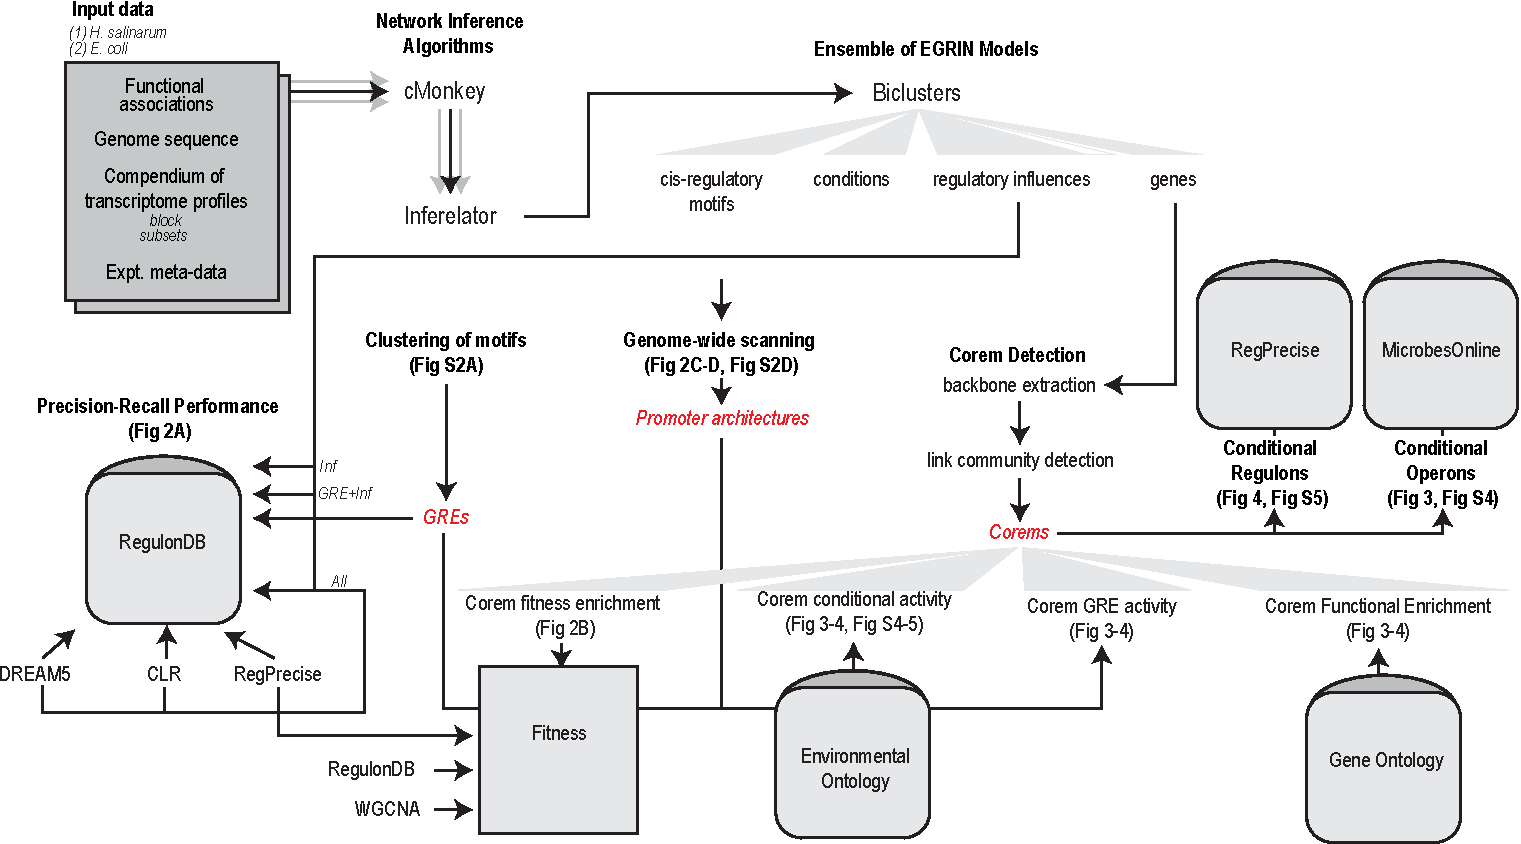
\includegraphics[width=\linewidth]{figures/workflow.pdf}
\caption[Detailed workflow for \egrine~inference procedure]{
{\bf Detailed workflow for \egrine~inference procedure.} Data input, processing and analysis to construct \egrine~model for {\it H. salinarum} and {\it E. coli}, and predictions generated. Predictions highlighted in individual figures are noted}\label{fig:workflow}
\end{figure}

% Table generated by Excel2LaTeX from sheet 'Table S2'
\begin{table}[htbp]
  \raggedright
    \begin{tabular}{|l|c|c|}
    \hline
    \textbf{Statistic} & \textit{\textbf{H. salinarum}} & \textit{\textbf{E. coli}} \\
    \hline
    %\midrule
    Arrays analyzed & 1495  & 868 \\
    Genes/transcripts & 2400  & 4213 \\
    Number of EGRIN models constructed & 572   & 106 \\
    Number of cMonkey biclusters & 142600 & 46520 \\
    Fraction of "good" cMonkey biclusters & 61\%  & 43\% \\
    Residual cutoff defining "good" biclusters & 0.40  & 0.55 \\
    Number of genes/transcripts in $\leq$ 1000 "good" biclusters (Hal) & 2104  &  \\
    Number of genes/transcripts in $\leq$ 200 "good" biclusters (Eco) &       & 4201 \\
    Average number of biclusters per gene & 1210  & 212 \\
    Number of motifs (total) & 269770 & 86167 \\
    Number of motifs (E-value $\leq$ 1) & 118546 & 15588 \\
    Number of motifs  (E-value $\leq$ 1e-6) & 32739 & 3506 \\
    Number of motif clusters & 162   & 402 \\
    Number of motifs contained in motif clusters & 37713 & 13519 \\
    Number of unique GREs & 135   & 337 \\
    Number of motifs in unique GREs & 27991 & 12773 \\
    Number of RegulonDB GREs detected (p $\leq$ 0.01) &       & 53 \\
    RegulonDB TFs with $\geq$ 3 experimentally characterized binding sites &       & 86 \\
    Corems & 679   & 590 \\
    Genes modeled by corems & 1363  & 1572 \\
    Genes per corem: min(max) & 3(377) & 3(153) \\
    Active conditions per corem: min(max) & 21(1279) & 69(598) \\
    GREs per corem: min(max) & 0(9)  & 0(12) \\
    Co-regulatory associations: prior to backbone extraction & 1573836 & 3094954 \\
    Co-regulatory associations: after backbone extraction & 141850 & 170723 \\
    Co-regulatory associations: corems & 56738 & 25976 \\
    \hline
    \end{tabular}%
    \caption{ Global properties of \textit{H. salinarum} and \textit{E. coli} ensembles}
  \label{tab:stats}%
\end{table}%

\subsection{Experimental Data}

\subsubsection{\halo~compendium}\label{halodata}

A compendium of 1495 transcriptome profiles were collated from a wide array of experiments conducted by our lab over the past decade that cover dynamic transcriptional responses to varied growth (1159 arrays), nutritional (161 arrays), and stress conditions (1102 arrays), including variation in temperature (256 arrays), oxygen (285 arrays), light (786 arrays), salinity (20 arrays), metal ions (274 arrays), and genetic perturbations (643 arrays).  We categorized the experiments using extensive metadata collected at the time of the experiment. We used this metadata to construct a GO-like ontology of the relationships between all experiments (discussed in detail below). The annotation counts above are derived from this resource (note that a single array can receive more than one annotation).  A full list of the metadata, annotations, and ontology is available on the web service.  1159 of the arrays are published (\cite{baliga_genome_2004,baliga_coordinate_2002,bonneau_predictive_2007,facciotti_large_2010,facciotti_general_2007,kaur_systems_2006,kaur_coordination_2010,schmid_two_2011,schmid_anatomy_2007,schmid_single_2009,whitehead_integrated_2006,whitehead_diurnally_2009}. 336 of the arrays are new for this study. Experimental protocols are identical to \cite{bonneau_predictive_2007}. These data, including expression levels (log$_2$ ratios vs. reference samples) and experimental metadata, are available online as a tab-delimited spreadsheet.

Each array in the {\it H. salinarum} compendium was collected using the same platform, using the same reference, and processed and normalized using the same protocol. More specifically, each RNA sample was hybridized along with a {\it H. salinarum NRC-1} reference RNA prepared under standard conditions (mid-logarithmic phase batch cultures grown at 37$^{\circ}$C in CM, OD = 0.5). Samples were hybridized to a 70-mer oligonucleotide array containing the 2400 non-redundant open reading frames (ORFs) of the {\it H. salinarum NRC-1} genome as described in \cite{baliga_genome_2004}. Each ORF was spotted on each array in quadruplicate and dye flipping was conducted (to rule out bias in dye incorporation) for all samples, yielding eight technical replicates per gene per sample. At least two independent biological replicates exist for all experimental conditions for a total of 16 replicates per gene per condition. Direct RNA labeling, slide hybridization, and washing protocols were performed as described by \cite{facciotti_general_2007,schmid_anatomy_2007}. Raw intensity signals from each slide were processed by the SBEAMS-microarray pipeline \cite{marzolf_sbeams-microarray:_2006} (www.SBEAMS.org/microarray), in which the data were median normalized and subjected to significant analysis of microarrays (SAM) and variability and error estimates analysis (VERA). Each data point was assigned a significance statistic, $\lambda$, using maximum likelihood \cite{ideker_testing_2000}.

\subsubsection{\eco~expression compendia}\label{ecodata}

\paragraph{\tmsamp{DISTILLER} expression compendium for model training}

A total of 868 \eco\ transcriptome profiles were compiled by \cite{lemmens_distiller:_2009} for use with their \tmsamp{DISTILLER} algorithm. These data were collated from publicly available microarray databases: 44 arrays from Stanford Microarray Database \cite{demeter_stanford_2007}, 617 from Gene Expression Omnibus \cite{barrett_ncbi_2007} and 36 from ArrayExpress \cite{parkinson_arrayexpresspublic_2007}, as well as 181 arrays from supplementary data in literature (for four different experiments). The experiments cover a range of conditions, including varying carbon sources (136 arrays), pH (46 arrays), oxygen (284 arrays), metals (27 arrays) and temperature (23 arrays). Overall, the compendium consists of measurements from single channel (407 arrays; including 298 Affymetrix, and 109 P33) and dual channel (460 arrays; including 337 DNA/cDNA and 126 oligonucleotide) platforms.

These microarray measurements were normalized by the authors \cite{lemmens_distiller:_2009}, as follows: ``If possible, raw intensities were preferred as data source over normalized data provided by the public repository. Dual-channel data were loess fitted to remove nonlinear, dye-related discrepancies. No background correction procedures were performed to avoid an increase in expression logratio variance for lower, less reliable intensity levels. Whenever raw data were available, single-channel data were first normalized per experiment with RMA. Logratios were then created for the single-channel data in order to combine them with the dual channel measurements. For each single-channel array, expression logratios were computed by comparing the normalized values against an artificial reference array.  This artificial reference array was constructed on a per experiment basis by taking the median expression of each gene across all arrays in the corresponding experiment. When deemed necessary (e.g. experiments normalized by MAS5.0 for which the raw data was not available), a loess fit was performed on these logratios. To ensure that the artificial reference was not altered by this intensity dependent non-linear rescaling, the artificial reference expression levels were chosen for the average log intensity (instead of the mean expression levels of the respective array and the artificial reference). To ensure comparability between arrays with a different reference, gene expression profiles were median centered across arrays that share the same reference. An additional variance rescaling of the gene expression profiles was performed to render genes with differing magnitudes of expression changes more comparable.''

The authors further note that, ``the array composition of the modules generated by \tmsamp{DISTILLER} is not biased towards arrays from any specific platform, indicating a correct preprocessing of the microarray compendium.'' \cite{lemmens_distiller:_2009} It is for this reason that we chose this normalized {\it E. coli} microarray compendium for \egrine~analysis.

\paragraph{\tmsamp{DREAM5} expression compendium for model validation}
\label{section:dream5_data_compendium}

To ascertain the generalizability of \egrine~models across data sets, we inferred a second \textit{E. coli} \egrine~model on an independent \textit{E. coli} gene expression compendium. By comparing this model to the original model we inferred using the \tmsamp{DISTILLER} data set, we were able (1) to understand what, if any, systematic biases exist due to normalization procedures, and (2) to cross-validate \egrine~predictions across two data set.

We obtained the de-anonymized {\it E. coli} microarray compendium from the \tmsamp{DREAM5} competition website \cite{marbach_wisdom_2012}. According to the authors, these data were ``compiled for {\it E. coli}, where all chips are the same Affymetrix platform, the \textit{E. coli} Antisense Genome Array. Chips were downloaded from GEO (Platform ID: GPL199). In total, 805 chips with available raw data Affymetrix files (.CEL files) were compiled.''  Additionally, ``Microarray normalization was done using Robust Multichip Averaging (RMA) 9 through the software RMAExpress. All 160 chips were uploaded into RMAExpress and normalization was done as one batch. All arrays were background adjusted, quantile normalized, and probesets were summarized using median polish. Normalized data was exported as log-transformed expression values. Mapping of Affymetrix probeset ids to gene ids was done using the library files made available from Affymetrix. Control probesets and probesets that did not map unambiguously to one gene were removed, specifically probeset ids ending in \_x, \_s, \_i were removed. Lastly, if multiple probesets mapped to a single gene, then expression values were averaged within each chip.''

Compared to the \tmsamp{DISTILLER} \cite{lemmens_distiller:_2009} data set, the \tmsamp{DREAM5} \cite{marbach_wisdom_2012} compendium contained a different subset of the available \textit{E. coli} transcriptome measurements from a different combination of platforms. While one might expect a number of arrays to be common between the two compendia, we discovered that the two data sets differed substantially in their statistical properties. The maximum Pearson correlation between arrays across the two data sets, for example, was $\sim 0.63$. Interestingly, the correlation among expression profiles of genes within predicted operons \cite{price_novel_2005} was higher in the \tmsamp{DREAM5} compendium (mean $\sim 0.83$) than the \tmsamp{DISTILLER} compendium (mean $\sim 0.32$). This is likely due to a combination of differences in the experiments/platforms included and normalization procedures.

\subsubsection{Additional Data}

\paragraph{Genome sequence data and annotations for \cm~analysis}

We used genome sequences and gene annotations (coding regions) collated in \tmsamp{RSA-tools} \cite{van_helden_web_2000} for both organisms in this study (\halo~and \eco). These data were themselves collated to annotate regulatory sequences of all sequenced genomes in \tmsamp{RefSeq}. Rather than using the \tmsamp{RSA-tools}-annotated promoter regions, we computed them ourselves as regions (-250 nt to +50 nt) surrounding the annotated translation start site of each gene/operon (see below for operon annotations).

In all cases where probe identifiers in the mRNA expression compendia used for this analysis could not be directly matched to gene annotations (or operon predictions or functional associations; see below), we used the \tmsamp{RSA-tools} ``\tmsamp{feature\_names.tab}''table of identifier synonyms to perform the match. In cases where the match was still not possible, we excluded the probe/ annotation/ association from analysis.

\paragraph{Operon membership predictions used for \cm~analysis}

We used operon predictions for both \halo~and \eco~predicted by \cite{price_novel_2005} from the \tmsamp{Microbes Online} database \cite{alm_microbesonline_2005}. These predictions are updated regularly. The predictions are based upon genomic proximity and co-expression in publicly-available microarray data compendia. We used the versions downloaded from the website as of March, 2009. These included predicted operon memberships for 826 genes in \halo~ and for 2,639 genes in \eco.

\paragraph{Predicted transcriptional regulators used for \nwinf~analysis}

\paragraph{\halo}

For \halo, we used the same set of putative transcription factors (TFs) as \cite{bonneau_inferelator:_2006,bonneau_predictive_2007}. This list of 124 regulators was selected from among the 2,400 \halo\ genes which are annotated as known or putative TFs based upon sequence or predicted structural homology \cite{bonneau_comprehensive_2004}.

\paragraph{\eco}
\label{section:eco_tfs}

To enable direct comparison of our results to DREAM5, we used the list of 296 putative \eco~ transcriptional regulators collated by \cite{marbach_wisdom_2012}. Their list was obtained by combining the list of TFs defined by RegulonDB \cite{gama-castro_regulondb_2011} with TFs identified using Gene Ontology (GO) terms: \textit{biological process} terms related to transcription (\texttt{GO:0009299;mRNA transcription} or \texttt{GO:0006351;transcription, DNA dependent}) and GO \textit{molecular function} \texttt{GO:0003677;DNA binding} or any child terms.

\paragraph{Functional association networks integrated into \cm~analysis}

We used EMBL STRING \cite{szklarczyk_string_2011} v9.0 database of predicted functional associations between genes for both organisms (\halo~and \eco) to constrain module construction in \cm, as described below. The confidence scores estimated by \cite{szklarczyk_string_2011} were incorporated into the \cm~constraints. These networks included 151,826 associations among 2,559 genes in \halo, and 878,972 associations among 4,136 genes in \eco.

%\subsubsection{Statistical mining of the relationships in the ensemble}
\subsection{\egrine: an ensemble of EGRINs, generation and statistical mining}

\egrine~model construction and analysis was performed using primarily the \tmsamp{R} statistical analysis environment, with add-on packages \tmsamp{data.table} and \tmsamp{filehash} for off-line storage (maintaining all information in memory was impossible for our large ensembles). Once the full set of \cm\ and \nwinf\ runs were completed and stored, a round of post-processing was performed to agglomerate all results into a single ad-hoc database for storage and query. The following relationships could be queried to identify significant associations between biological entities described in the model:\\

\begin{tabular}{|l|l|l|r|} 
\hline
Entity$_1$        & Entity$_2$         & Relationship  & Associated info. \\ \hline
Bicluster         & Gene               & Contains      & - \\
Bicluster         & Condition          & Contains      & - \\
Bicluster         & Motif              & Contains      & Associated genes \\
Regulator         & Bicluster          & Regulates     & Weight \\
Motif             & Motif              & Similar       & $FDR\ q$--value \\
Motif             & Genomic coordinate & Overlaps      & $p$-value \\
\hline
\end{tabular}
\\

\noindent These relationships could then be extended to second-degree relationships, including (these relationships below are by no means all-inclusive; for brevity we denote $g$, $g_1$, and $g_2$ as separate genes, $b$ as a bicluster, $m$ as a motif, $r$ as a regulator, and $c$ as an experimental condition):

\begin{enumerate}
\item $g_1$ is co-regulated with $g_2$ if they occur in the same $b$.
\item $g_1$ is co-regulated with $g_2$ under condition $c$ if $g_1$, $g_2$, and $c$ occur in the same $b$.
\item $m$ regulates $g$ if $m$ and $g$ are both observed in the same $b$.
\item $m$ regulates $g$ under condition $c$ if $m$, $g$, and $c$ are all observed in the same $b$.
\item $r$ putatively regulates gene $g$ via $m$ if $r$ is predicted to regulate $b$ which contains both $g$ and $m$.
\end{enumerate}

\noindent The frequency with which any of these relationships occurs throughout the entire ensemble of EGRIN models could subsequently be counted by querying the database, and a $p$-value describing the significance of the frequency computed via the cumulative hypergeometric distribution. $p$-values were then converted to false discovery rate $q$-values using the Benjamini–Hochberg procedure.  We use this basic procedure to identify conditions associated with GRE influence, and GREs associated with gene co-regulation, as we describe below.

\subsection{Clustering of \textit{cis}-regulatory motifs to identify GREs}
\label{section:gres}

Each \cm~ bicluster contains at least one {\it de novo} \MEME - detected \cite{bailey_methods_1998} {\it cis}-regulatory motif. These motifs are used by \cm~ to guide bicluster optimization (in addition to other scoring metrics). There were 86,167 and 269,770 motifs detected across the entire ensemble for {\it E. coli} and {\it H. salinarum}, respectively. Each motif was represented in the model as a position-specific scoring matrix (PSSM). To determine which of these motifs represented \textit{bona fide} GREs (as opposed to false positives), we computed pairwise similarities between all motifs using \tmsamp{Tomtom} \cite{gupta_quantifying_2007} (Euclidean distance metric; minimum overlap of 6 nt) and clustered the most highly similar PSSM pairs using \tmsamp{mcl} \cite{van_dongen_using_2012}.

The \tmsamp{Tomtom} motif similarity $p$-value threshold and the \tmsamp{mcl} inflation parameter ($I$) were selected to (1) maximize the density (unweighted) of edges between PSSMs inside clusters relative to the edges between clusters, and (2) ensure that the \tmsamp{mcl} ``jury pruning synopsis'' was at least 80 (out of 100). Criterion (1) aims to find a clustering that is as inclusive as possible, while minimizing over-clustering, while (2) is a built-in mcl metric that evaluates the quality of the clusters resulting from the user-selected pruning strategy ($I$). More specifically for criterion (1), we chose the clustering parameters (\tmsamp{mcl} inflation parameter $I$, \tmsamp{Tomtom} $p$-value cutoff $p_c$) which maximize:

\begin{equation}
\label{eq:motif:clust}
\left( I, p_c\right) = \arg \max \left\{ \sum_{I=1}^N \sum_{i=1}^{n_I} \frac{ \sum_{j=1}^{n_I} \delta_{ij} }
                            { \sum_{J=1}^N \sum_{k=1}^{n_J} \delta_{ik} } \right\},
\end{equation}

\noindent where $N$ is the total number of motif clusters for a given set of parameters, $\delta_{ij}$ indicates a significant similarity (subject to the given $p$-value threshold) the between PSSMs $i$ and $j$ within motif cluster $I$ (which contains a total of $n_I$ PSSMs), and $\delta_{ij}$ indicates a significant similarity between PSSM $i$ in motif cluster $I$ and PSSM $j$ in motif cluster $J$. The final parameters that maximized expression~\ref{eq:motif:clust} and resulted in an \tmsamp{mcl} ``jury pruning synopsis'' of at least 80 were different for the two \egrine~models: $p_c = 10^{-6}$ and \tmsamp{mcl} $I = 4.5$ for the {\it H. salinarum} ensemble and $p_c = 10^{-5}$ and \tmsamp{mcl} $I = 1.5$ for the {\it E. coli} ensemble.

We did not filter the motifs by $E$-value or other intrinsic motif quality metrics; rather, we enforced a cluster size threshold to ensure that GREs were re-detected consistently. Clusters containing at least 10 PSSMs were considered GREs. This criterion resulted in 135 GREs for {\it H. salinarum} (representing 27,991 PSSMs, Table S2\footnote{All tables refer to Tables available in \cite{brooks_systemlevel_2014} and \href{http://egrin2.systemsbiology.net}{online}}) and 337 for {\it E. coli} (representing 12,773 PSSMs, Table S3). Finally, we computed a ``combined PSSM'' for each GRE as the unweighted mean of aligned PSSMs within each cluster. This combined PSSM could be visualized as a motif logo identically to standard motif PSSMs.

The motif clustering procedure is summarized in Figure \ref{fig:gre_clustering}. 

\begin{figure}[h!]
\centering
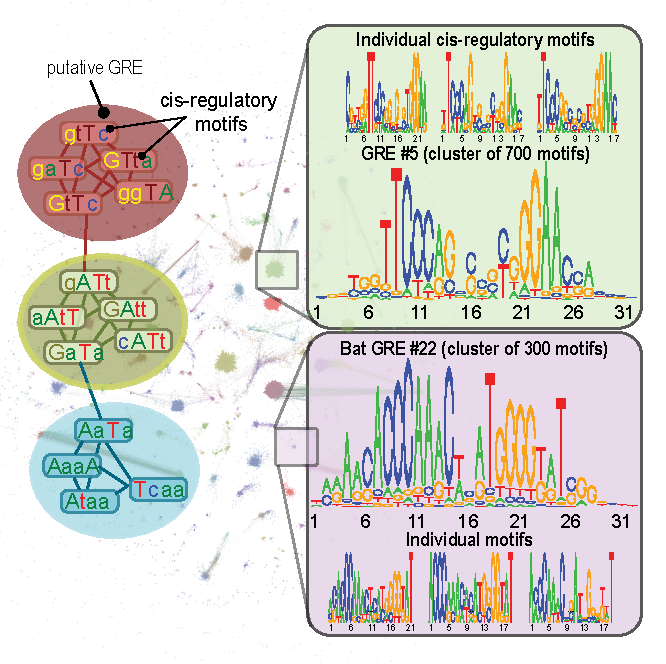
\includegraphics[width=0.6\linewidth]{figures/gre_clustering.pdf}
%\epsfig{file=figures/e2.eps,width=0.8\linewidth}
%\vspace{5in}
\caption[Motif clustering and GRE identification]{
\textbf{Motif clustering and GRE identification.} (Left) A schematic of the approach used to align and cluster individually detected motifs to define GREs. In this example, similar motifs were aligned and clustered into three GREs using Tomtom and mcl (Details in Methods and Supplementary Methods). (Center) The {\it H. salinarum} network of aligned and clustered motifs. (Right) Two {\it H. salinarum} GREs discovered by this method. The motif logo of each GRE was generated by summing PSSMs of the individual aligned motifs in the cluster, as illustrated by three examples of individual motifs (prior to alignment) for each of the two GREs. Note that relative to the individual motifs, the averaged GRE motif is more palindromic - a hallmark of binding sites for dimeric TFs.}
\label{fig:gre_clustering}
%\vspace{-.1in}
\end{figure}

\subsection{Genome-wide scanning of motifs to obtain GRE locations}
\label{section:scanning}

We used motif scanning to discover GRE locations that were missed by the rigid definition of a promoter in \cm\ (typically -250 to +50 nucleotides surrounding the translation start site). This procedure was critical for discovering GREs in non-canonical locations, such as internal to operons. We computed how well each PSSM (described above) matched every position in the genome using \tmsamp{MAST} \cite{bailey_methods_1998}, and recorded significant matches at each genomic location subject to a position $p$-value threshold of $10^{-5}$. This $p$-value cutoff corresponds to an expectation of discovering $\sim 20$ sites at random across the genome. For each GRE, we summed the number of significant matches to each of the GRE’s PSSMs at each genomic position. These counts were used to represent GRE composition in promoters (Figure \ref{fig:egrin2:2:C} and Figure \ref{fig:egrin2:2:D}). In addition, we used these scanned locations to identify GREs located predominantly inside coding regions. Since these GREs may be spurious (\eg, protein sequence motifs or trinucleotide patterns) they were flagged, although they were not removed from our global analysis.

We compared the genome-wide distribution of GRE locations to annotated start sites in \textit{H. salinarum}.  We discovered that most GREs occur in consistent locations with respect to gene start sites.  The global position of all GREs and select GREs relative to experimentally determined gene start sites is depicted in Figure \ref{fig:gre_global_locs_hal}.

\begin{figure}[h!]
\centering
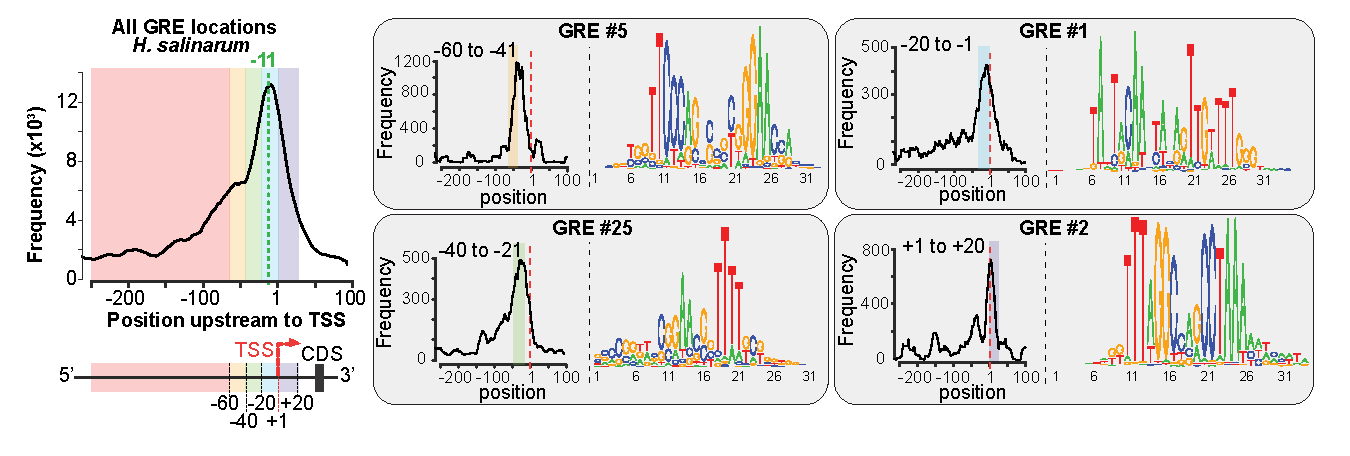
\includegraphics[width=0.95\linewidth]{figures/gre_global_locs_hal.pdf}
\caption[Genome-wide distribution of GREs relative to experimentally mapped transcriptional start sites in \textit{H. salinarum}]{\textbf{Genome-wide distribution of GREs relative to experimentally mapped transcriptional start sites in \textit{H. salinarum}.}  (Left) Predicted positions for all GREs in gene promoters upstream of experimentally mapped transcription start sites (TSSs; \cite{koide_prevalence_2009}) in and (Right) four example elements. Distribution peaks for most GREs occur at characteristic locations. For instance, the location of TATA box-like elements (GRE \#25) between -21 to -40 nt upstream to TSSs in {\it H. salinarum} is consistent with the characterized location of basal elements in archaeal promoters (-25 to 30 nt upstream to TSS). GRE location enables prediction of putative roles for the cognate TF (\eg repressor, activator or a basal factor).} 
\label{fig:gre_global_locs_hal}
\end{figure}

\subsection{Detection of co-regulated modules (corems) by community detection}

\subsubsection{Construction of gene-gene co-occurrence network}
\label{section:gBg}

We post-processed the \egrine~ensemble to refine the underlying network structure and discover functionally meaningful gene co-regulatory modules present in the model. To do so, we transformed the ensemble of biclusters into a weighted gene-gene association graph $G$, where the nodes of $G$ are genes and the weight of edges between the nodes is proportional to their frequency of co-occurrence in biclusters:

\begin{equation}
w_{ij} = \frac{\left|B_i\cap B_j\right|}{\mathrm{min}(B_i,B_j)},
\end{equation}

\noindent where $w_{ij}$ is the weight of the edge between genes $i$ and $j$, $B_i$ is the set of all biclusters containing gene $i$. The weights were normalized by the minimum number of biclusters containing either gene, rather than by the more typically applied union (which would make the score identical to the Jaccard Index) to avoid penalizing genes that occur infrequently in biclusters. The sum of edge weights for each gene was normalized to one. This gene-gene co-occurrence network represents how often \cm~ discovers co-regulation between every pair of genes in the genome. We note that since this network is derived from biclusters, it is also a reflection of conditional co-expression and predicted \textit{cis}-­regulatory motifs.

\subsubsection{Network backbone extraction}

After transforming the ensemble into a normalized graph, we removed edges that were statistically indistinguishable by multiscale backbone extraction (null hypothesis of uniform edge weight distribution given a node of degree $k$) \cite{serrano_extracting_2009}. We retained all edges satisfying the following relation:

\begin{equation}
\alpha_{ij}=1-(k-1)\int_0^{w_{ij}}(1-x)^{k-2}dx\leq 0.05,
\end{equation}

\noindent where $\alpha_{ij}$ is the probability that the normalized weight $w_{ij}$ between genes $i$ and $j$ is compatible with the null hypothesis, and $k$ is the degree of gene $i$. For \halo, backbone extraction reduced the number of regulatory edges from 1,576,643 to 141,667; in \eco~ the number of edges was reduced from 3,094,954 to 170,723.

\subsubsection{Network link-community detection}
\label{section:linkcommunity}
Following backbone extraction, we detected corems by application of a recently described link-community detection algorithm \cite{ahn_link_2010}. For this algorithm to work on our data set we modified it to accept input of a weighted graph \cite{kalinka_linkcomm:_2011}. We implemented it in \tmsamp{C++} for efficiency. The algorithm computes a similarity score between all pairs of edges sharing a common keystone node, $k$, according to the Tanimoto coefficient, $T$:

\begin{equation}
T(e_{ik},e_{kj}) = \frac{a_i\cdot a_j}{|a_i|^2+|a_i|^2+a_i\cdot a_j},
\end{equation}

\noindent where

\begin{equation}
a_i=w_{ij}+\frac{\delta_{ij}}{k_i}\sum_{l\in n(i)}w_{il}.
\end{equation}

\noindent Here, $e_{ik}$ is the edge between gene $i$ and the keystone gene $k$, and $\delta_{ij}$ is the Kroenecker delta. The score reflects the similarity of gene neighborhoods adjacent to two edges sharing a gene, with the score increasing in value as the number and weight of overlapping adjacent edges increases. To transform the Tanimoto coefficient into a distance metric, we compute $1-T$.

Following scoring, the edges were aggregated by standard hierarchical clustering. The resulting tree is cut at many thresholds to optimize the local weighted density $D$ of the resulting clusters:

\begin{equation}
D=\frac{1}{M\langle w\rangle}\sum_{c\in C}m_c\langle w\rangle_c\left(\frac{m_c-(n_c-1)}{n_c(n_c-1)/2-(n_c-1)}\right),
\end{equation}

\noindent where $M$ is the total number of edges in the entire network, $\langle w\rangle$ is the average weight of edges in the entire network, $C$ is the set of all link communities at a given threshold, $m_c$ is the number of edges in community $c$, $\langle w\rangle_c$ is the average weight of edges in community $c$, and $n_c$ is the number of genes in community $c$. The density scoring metric $D$ had a clear optimum corresponding exactly to the cutoff that would have been chosen had we used the unweighted scoring metric originally described (Figure \ref{fig:corem_density}). Only communities with more than two genes were retained.

\begin{figure}[h!]
\centering
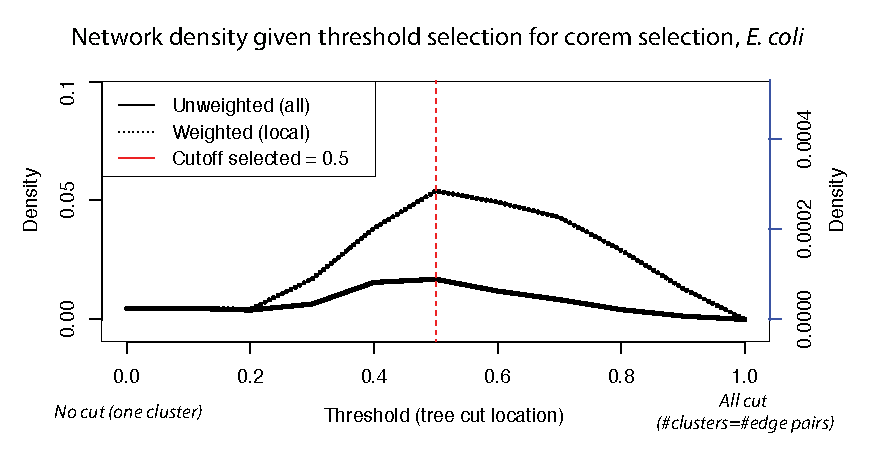
\includegraphics[width=0.9\linewidth]{figures/corem_density.pdf}
\caption[Corem density as a function of clustering cutoff threshold]{{\bf Corem density as a function of clustering cutoff threshold.} Hierarchical clustering cut threshold chosen to maximize the density of resulting clusters. The cutoff chosen with modified weighted density metric is identical to unweighted density metric.} 
\label{fig:corem_density}
\end{figure}

Since the communities produced by this algorithm are comprised of sets of edges, we defined a corem to include all genes incident to the edges in a community. Because of this definition, each gene can be a member of multiple different corems. In {\it H. salinarum}, this procedure generated 679 corems ranging in size from 3 to 377 genes, covering 1,363 of the 2,400 genes in the genome, and comprising 56,738 co-regulatory associations. In {\it E. coli}, we discovered 590 corems, ranging in size from 3 to 153 genes, covering 1,572 of 4,213 genes and 25,976 regulatory edges. See Table\ref{tab:stats} and Figure \ref{fig:corem_density} for additional statistics. Gene-to-corem and corem-to-gene mappings for the {\it H. salinarum} and {\it E. coli} models are available online.

\begin{figure}[h!]
\centering
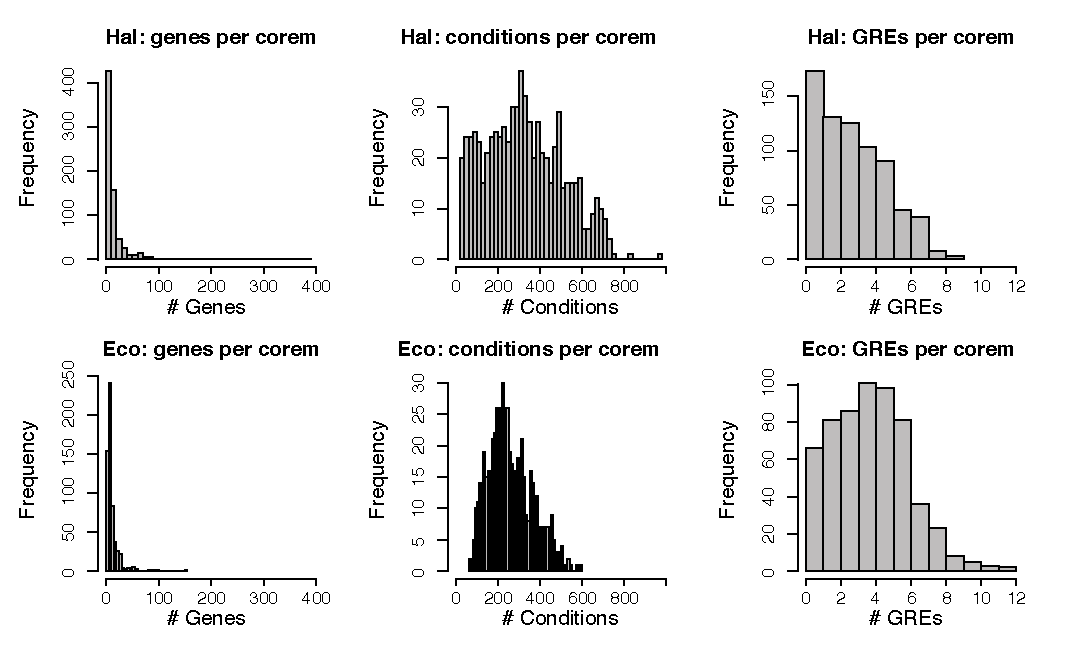
\includegraphics[width=0.9\linewidth]{figures/corem_stats.pdf}
\caption[Corem statistics]{
{\bf Corem statistics.} Number of genes, conditions, and GREs per corem for \textit{E. coli} and \textit{H. salinarum} \egrine~models.} 
\label{fig:corem_stats}
\end{figure}

\section{Model Evaluation}

In this section we evaluate the performance of the \egrine\ model as a function of several important parameters. We focus in particular on how the performance of the model changes as a function of the number of runs included. From these evaluations, we conclude that (1) the model performs well in its final form, (2) the model has reached a stable-state wherein inclusion of additional runs does not significantly increase model performance, and (3) the model is not over-fit to particular experiments within a data set or to any data set as a whole.

\subsection{Comparison with other module detection algorithms}

We compared the number of \rdb~TFs detected in the \egrine~model to individual \cm~runs as well as to several other module detection/clustering algorithms that were computed on subsets of the experimental data (similar to the \egrine~ensemble; Figure \ref{fig:ensemble_comparison_regDB}). We evaluated: (a) $k$-means clustering, (b) \tmsamp{WGCNA} \cite{langfelder_wgcna:_2008}, and (c) \tmsamp{DISTILLER} \cite{lemmens_distiller:_2009}. For (a) and (b), we computed modules 100 times on random subsets of the {\it E. coli} expression data set (using 200-250 randomly chosen experiments per run; selection criteria were identical to {\it E. coli} \egrine). We then predicted {\it de novo cis}-regulatory GREs in the promoter regions of genes in each module using \tmsamp{MEME} (\tmsamp{MEME} parameters were also identical to \egrine). For (c), we performed the comparison using the original modules generated by \cite{lemmens_distiller:_2009}. Rather than alter module composition by re-detection, we instead varied \tmsamp{MEME} parameters applied to the modules 100 times (again, within the same ranges as those used for \egrine). TF-GRE matches were assigned by comparing GREs to \rdb~TF binding sites, as previously described (Section~\ref{section:tfbs:vs:regdb}).

We found that individual \cm~runs discovered a greater number of \rdb~binding sites, on average, than the other methods (an average of 41 for \cm, compared to averages of 30, 25, and 29 for $k$-means, \tmsamp{WGCNA}, and \tmsamp{DISTILLER}, respectively), which is consistent with previous findings \cite{reiss_integrated_2006} (Figure~\ref{fig:ensemble_comparison_regDB}). Integration of all \cm~biclusters into the complete \egrine~ensemble outperformed all individual \cm~runs (53 total, as described in the Manuscript). This result is typical of ensemble-based inference approaches, and supports the value of ensemble integration as part of the \egrine\ model.

\begin{figure}[h!]
\centering
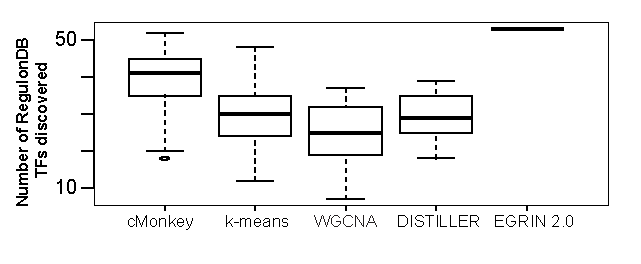
\includegraphics[width=0.6\linewidth]{figures/ensemble_comparison_regDB.pdf}
\caption[Number of TFs in \rdb~ re-discovered by various regulatory module detection methods.]  {{\bf Number of TFs in \rdb~ re-discovered by various regulatory module detection methods.} Comparison of \egrine~ (solid line, far right) to individual \cm\ runs, as well as multiple runs of $k$-means, \tmsamp{WGCNA}, and \tmsamp{DISTILLER} on subsets of the expression data. Evaluation made with respect to re-discovery of binding sites for 88 TFs with $\geq 3$ unique sites in \rdb~ based on genome-wide binding site locations (FDR $\leq 0.05$).} 
\label{fig:ensemble_comparison_regDB}
\end{figure}

\subsection{Convergence and stability of inferred GRNs}

To evaluate the stability of the inferred \egrine\ network, we quantified how the model changes as individual \cm\ runs are excluded from the ensemble. Since the sub-bagging, as performed for the \egrine\ model inference, reduce model over-fitting, we used this evaluation understand whether the model is over-fit to particular experiments in the data set. For this task, we computed the number of individual EGRIN runs required to converge on a consistent gene-gene co-occurrence network (see Section \ref{section:gBg}). We computed gene-gene co-occurrence networks based upon randomly selected subsets of the 106 available \eco\ \cm\ runs, and varied the percentage selected between 1\%-99\% of the 106 runs. 5 replicate samples were computed for each. To compare the networks, we computed the Pearson correlation between the two matrices (sub-sampled gene-gene co-occurrence versus the final \egrine\ gene-gene co-occurrence network). Note that since the gene-gene co-occurrence network is a weighted adjacency matrix, the correlation reflects the weighted discovery rate for every pair of genes (rather than simple presence/absence). In Figure \ref{fig:gBg_network_converge} we demonstrate that the underlying networks converge rapidly to the final solution. By the time $\sim 50$\% of the runs have been included ($\sim 50$ runs), the inferred network is nearly identical to the final network ($\sim 100$ runs; cor $> 0.9$). The backbone extracted network takes a slightly longer time to converge, likely because it requires more observations of gene-gene pairs to retain them in the final network. Since corem detection is deterministic and strictly based on the underlying gene-gene co-occurrence matrix, this convergence means that the inferred corems would be nearly identical even if up to half of the runs were excluded.

\begin{figure}[h!]
\centering
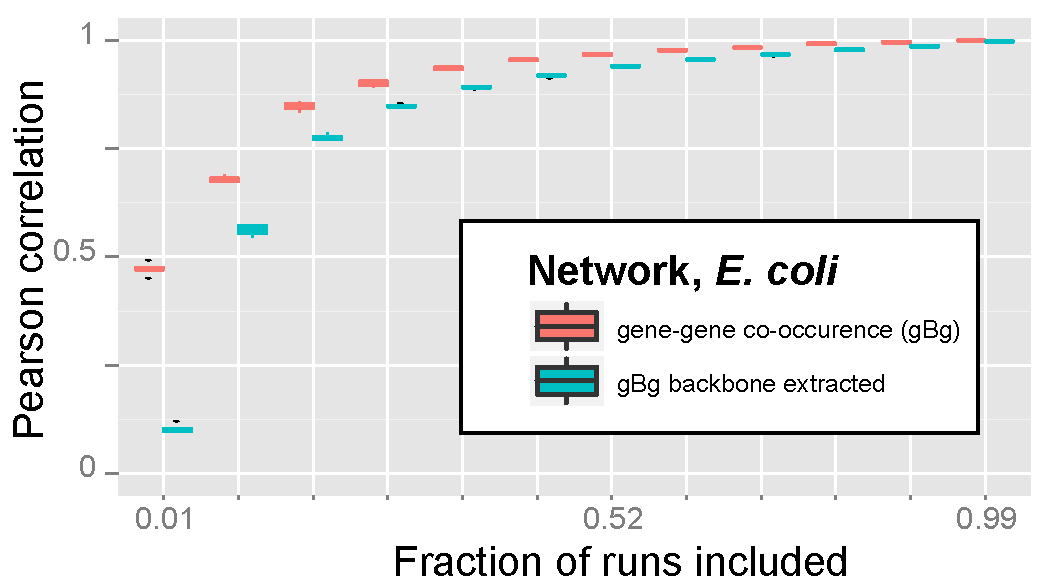
\includegraphics[width=0.75\linewidth]{figures/gBg_network_converge.pdf}
\caption[Convergence of \egrine\ gene co-occurrence networks.]  {{\bf Convergence of \egrine\ co-occurrence networks.} The co-regulation of genes predicted by the \eco\ \egrine\ model converges rapidly to a stable network. Shown is the similarity of the gene-gene co-occurrence matrix (and the backbone extraction of this matrix) to the final \egrine\ \eco\ network, computed when varying fractions of the \cm\ runs were excluded (Pearson correlation vs. the complete model). Each point contains a box plot representing 5 replicate sub-samples.} 
\label{fig:gBg_network_converge}
\end{figure}

\subsection{Confirmation of corems in an independent data set}

To determine whether \egrine\ model predictions are over-fit to the \tmsamp{DISTILLER} expression compendium (or are the result of biases in that data set), we tested whether support for corems existed in an independent {\it E. coli} expression data set. Such evidence would suggest that corems are \textit{bona fide} gene regulatory modules that can be re-discovered in independent data, and that their degree of condition-specificity is not biased due to normalization differences in any given data set. For this test, we used the \tmsamp{DREAM5} gene expression compendium. As described above (Section \ref{section:dream5_data_compendium}), this data set is comprised of different conditions, array platforms, and, most important, was normalized by different methods, than the \tmsamp{DISTILLER} data set used for model training. We determined the condition-specific activity of corems in the \tmsamp{DREAM5} data set using the methods described in Section \ref{section:rsd}. If a corem was significantly co-expressed ($p$-value $\leq$ 0.05) in at least one condition, we classified it `supported'. To our surprise, we not only discovered support for $\sim 99$\% of the predicted corems, we also discovered that their conditionality was very similar across both data sets -- \ie, corems discovered to be co-expressed in few conditions in the \tmsamp{DISTILLER} data set are also co-expressed in few conditions in the \tmsamp{DREAM5} data set (same for corems regulated in many conditions), and similarly for corems co-expressed in a large number of conditions (Figure~\ref{fig:corem_conds_distiller_dream5}). Even after we removed the intrinsic relationship between the number of genes in a corem and the number of conditions in which it is co-expressed, we still observed a significant partial correlation of 0.49 ($p$-value $< 10^{-6}$) between the number of conditions in corems as defined from the two data sets.

\begin{figure}[h!]
\centering
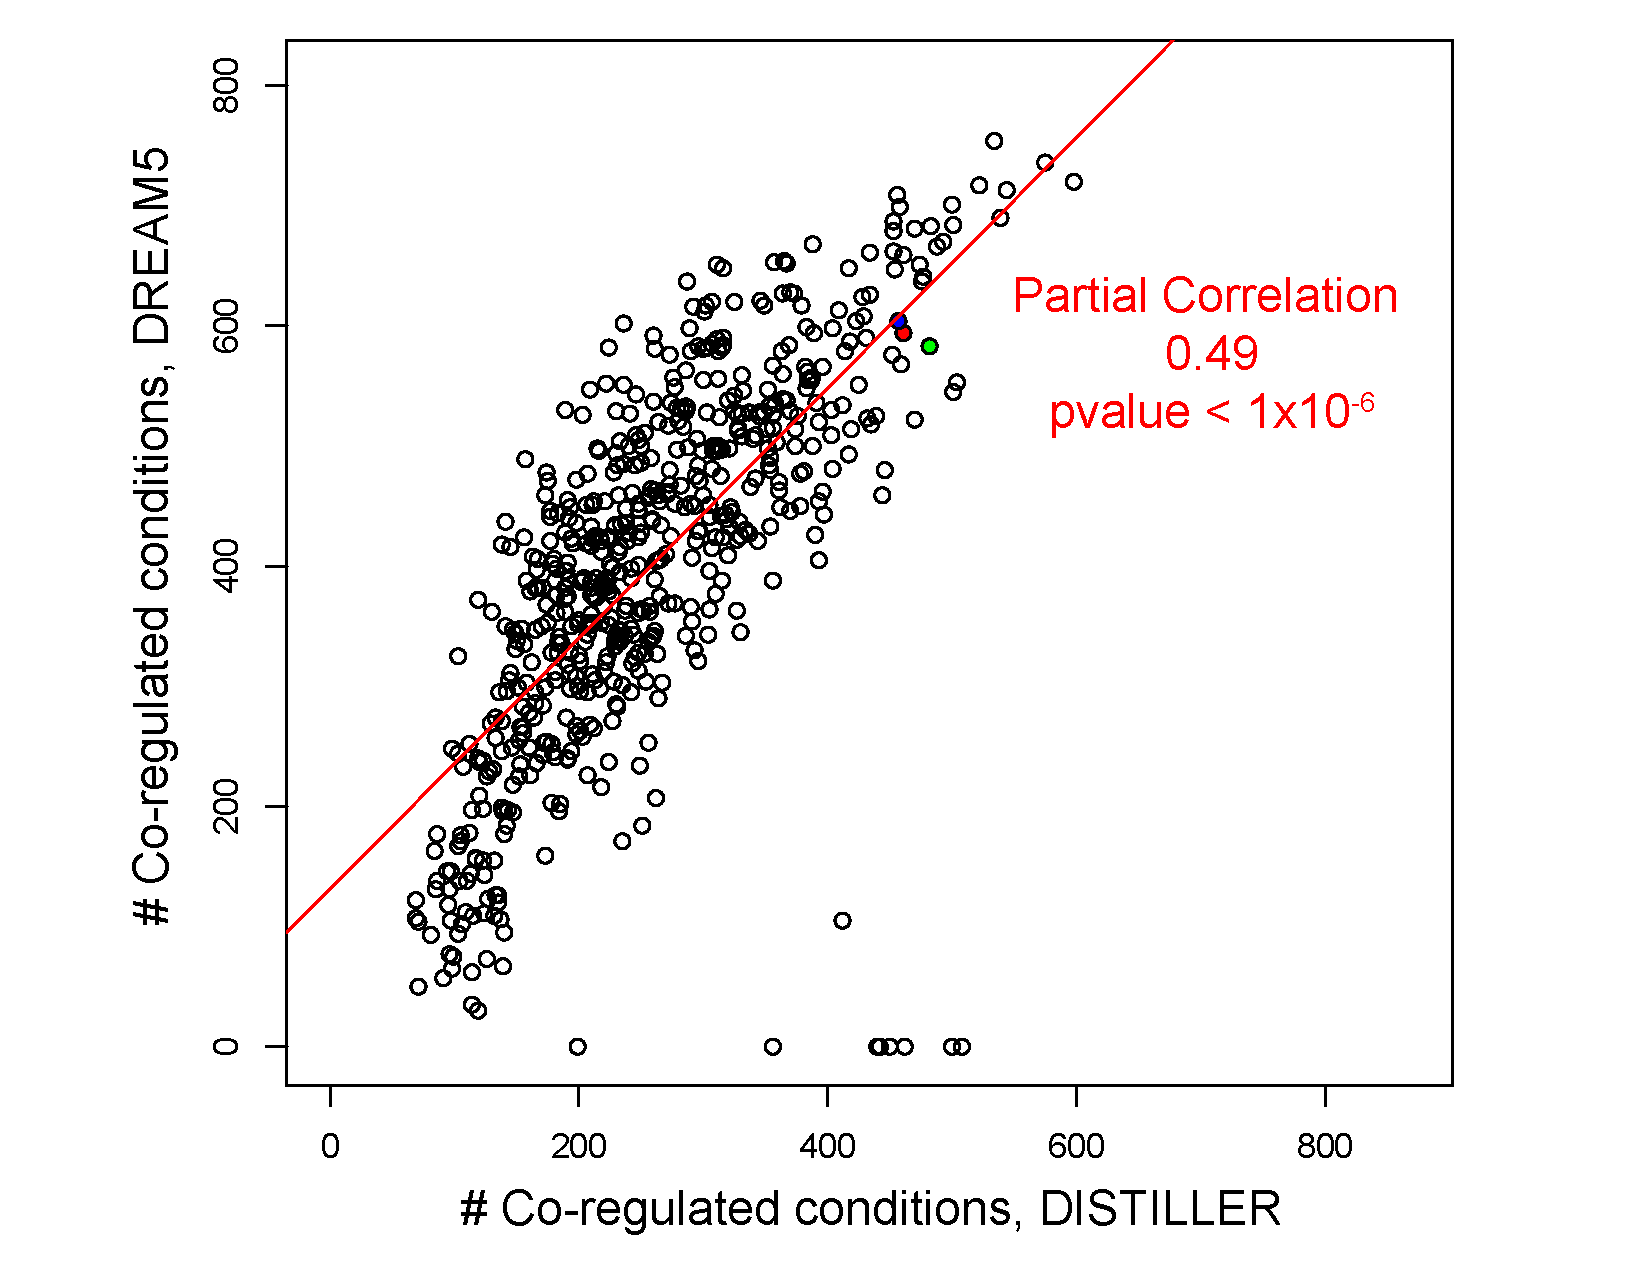
\includegraphics[width=0.6\linewidth]{figures/corem_conds_distiller_dream5.pdf}
\caption[Reproducibility of corems across data sets]{\textbf{Reproducibility of corems across data sets.} Number of co-expressed conditions for corems in the \tmsamp{DISTILLER} and \tmsamp{DREAM5} expression compendia. Conditions were selected as in Section~\ref{section:rsd}. Significant partial correlation of 0.49 is observed after removing the affect of gene set size (log) on the number of conditions co-expressed ($p$-value $< 10^{-6}$). The three corems detailed in the main manuscript are identified with their respective colors ({\color{red}ec512157}, {\color{blue}ec516034}, {\color{green}ec516031})} 
\label{fig:corem_conds_distiller_dream5}
\end{figure}

\section{Model Validation}

\subsection{Data For Model Validation}

\subsubsection{ \halo} \label{halodata}

\paragraph{Tiling array transcriptome measurements}

We generated {\it H. salinarum NRC-1} high-resolution (12 nt) tiling array transcriptome measurements over 12 points along the growth curve in rich media. These were analyzed and published in a separate study \cite{koide_prevalence_2009}. Locations of putative transcription breaks in these data were identified in using multivariate recursive partitioning, including signals from both relative changes in expression along the growth curve, as well as raw RNA hybridization signal.

\paragraph{ChIP-chip transcription factor binding measurements for global regulators}

Global binding of eight general transcription factors (seven TFBs [TFBa, TFBb, TFBc, TFBd, TFBe, TFBf, and TFBg] and one TBP [TbpB]) and three specific TFs (Trh3, Trh4, and VNG1451C) in {\it H. salinarum} were collected in our lab by ChIP-chip. A detailed protocol is described in \cite{facciotti_general_2007}. Briefly, ChIP-enriched and amplified DNA for eleven regulators was hybridized to a low-resolution (500~nt resolution) custom PCR-product array spotted in-house. The resulting intensities were analyzed using {\tmsamp{MeDiChI}} \cite{reiss_model-based_2008} to obtain binding site locations with an average precision of 50~nt. Local false discovery rates (LFDRs) were quantified by simulation.

\paragraph{\textit{kdp} promoter serial truncation measurements}

{\it H. salinarum NRC-1} \textit{kdpFABC} truncation data were obtained from \cite{kixmller_archaeal_2011}. Briefly, the authors measured relative induction of a transcriptional reporter after serial truncation of the \textit{H. salinarum} R1 \textit{kdpFABC} promoter. The authors measured $\beta$-Galactosidase activities from truncated transcriptional fusions of the \textit{kdpFABC} promoter to \textit{bgaH}. $\beta$-Galactosidase activities were measured in triplicate from cultures grown in inducing (3 mM K$^{+}$) and non-inducing (100 mM K$^{+}$) conditions. We obtained data corresponding to Figure \ref{fig:egrin2:2:C}, in which the authors quantify the fractional $\beta$-Galactosidase activity (non-induced/induced) among the serial truncations (private communication). We overlaid motif predictions from \egrine~on this data set to reach our conclusions.

\subsubsection{\eco} \label{ecodata}

\paragraph{Tiling array transcriptome measurements}
\label{section:ecoarray}

We measured \eco\ tiling array transcriptome profiles at nine different time points during growth in rich media (LB). Growth phases spanned lag-phase (OD600 = 0.05) to late stationary-phase (OD600 = 7.3). RNA samples were prepared by hot phenol-chloroform extraction \cite{khodursky_escherichia_2003}. RNA was directly labeled and hybridized to custom Agilent tiling arrays containing 60mer probes tiled across both strands of the \eco\ genome using a sliding window of 23~nt (GEO Platform GPL18392), as in \cite{koide_prevalence_2009}. Expression measurements were quantile-normalized as in \cite{yoon_parallel_2011} and analyzed for condition-specific transcriptional isoforms following the segmentation protocol described in \cite{koide_prevalence_2009}. Data is available on GEO (GSE55879).

\paragraph{PurR/$\Delta$PurR expression data and ChIP-chip transcription factor binding sites} 

{\it E. coli} PurR/$\Delta$PurR expression data and ChIP-chip transcription factor binding measurements collected in the presence of adenine were taken from \cite{cho_purr_2011}. ChIP-chip relative intensities were re-analyzed using {\tmsamp{MeDiChI}} \cite{reiss_model-based_2008} to obtain binding site locations with an average precision of $\sim$25~nt.

\paragraph{Fitness measurements}
\label{section:fitness}

{\it E. coli} fitness measurements across 324 conditions were generated by \cite{nichols_phenotypic_2011}. In short, the authors quantitated growth rates for 3979 single gene deletions in each of 324 environments with variable stress, drug, and environmental challenges. \textit{E. coli} mutant colony sizes were quantified on agar plates.  Fitness correlations were obtained directly from the authors: \href{http://ecoliwiki.net/tools/chemgen/}{http://ecoliwiki.net/tools/chemgen/}. Each correlation value represents the Pearson correlation of fitness (\ie, relative growth rate) for pairs of single gene deletion mutants measured across all 324 conditions that are also present in our analysis. Relative fitness scores were also obtained directly from the authors.

\paragraph{Effector molecule measurements}

{\it E. coli} effector molecule measurements were taken from \cite{ishii_multiple_2007}. The authors measured metabolite levels using capillary electrophoresis time-of-flight mass spectrometry (CE-TOFMS) in \eco, as well as several other biomolecules (\eg., RNA and protein). \textit{E. coli} was grown in a chemostat at several different dilution rates (0.1, 0.2, 0.4, 0.5, and 0.7 hours$^{–1}$). We obtained the metabolite levels from the authors and computed Pearson correlation between metabolites assigned to regulate TFs by RegPrecise \cite{novichkov_regpredict:_2010}.

\paragraph{Experimentally mapped {\it E. coli} transcription factor binding sites}

We compared genome-wide locations of GREs in the {\it E. coli} EGRIN 2.0 model with experimentally-mapped binding sites from the \rdb database \cite{gama-castro_regulondb_2011}. To maintain consistency with our comparisons against the DREAM5 community networks \cite{marbach_wisdom_2012}, we used version 6.8 of the database. For binding sites, we used the {\tmsamp{BindingSiteSet}} table, filtered for only interactions with experimental evidence, and used only TFs with $\geq 3$ unique binding sites -- a total of 88 TFs.

\paragraph{Experimentally measured {\it E. coli} transcription factor regulatory targets}
\label{section:eco:gold:standard}

For the {\it E. coli} gold standard network, we used the same network as that used by \cite{marbach_wisdom_2012} for validation of the DREAM5 {\it E. coli} community predicted regulatory networks. This gold standard is based upon version 6.8 of the \rdb~ database \cite{gama-castro_regulondb_2011}, and only interactions with at least one strong evidence were included, for a total of 2,066 interactions. We mapped the $aaaX$-style gene names in the DREAM5 gold standard to the $b1234$ in \cm~using a translation table compiled in the {\tmsamp{EcoGene}} database, version 3.0 \cite{zhou_ecogene_2013}. We were able to map a total of 4,273 gene names. The final gold standard consisted of 2,064 interactions between 141 TFs and 997 target genes. The final, complete gold standard network used for all analyses is available \href{http://egrin2.systemsbiology.net/}{online}.

\subsection{Computational Methods for Model Validation}

\subsubsection{Functional enrichment estimates for genes in corems}

We computed functional enrichment for genes organized into corems using \tmsamp{DAVID} \cite{dennis_david:_2003} and the \tmsamp{DAVIDQuery} \cite{day_davidquery:_2010} \tmsamp{R}-package. Enrichments for each corem are available on the \href{http://egrin2.systemsbiology.net}{web site}.

\subsubsection{Conditional co-regulation of genes organized in corems}
\label{section:rsd}

We defined the conditions in which genes in a corem were co-regulated as the set of experiments in which the genes of a corem are more tightly co-expressed than one would expect at chance. We statistically evaluated tight co-expression using relative standard deviation (RSD $=|\sigma/\mu|$) by resampling. We chose RSD (rather than, for example, standard deviation, $\sigma$) to avoid over-weighting conditions in which the mean relative expression is close to zero. The significance of an RSD value for a given condition relative to each corem was estimated by resampling: for a corem with $k$ gene members, and for each condition, $c$, we computed at least 20,000 RSD values for $k$ randomly sampled expression measurements in $c$, to determine the likelihood that the observed co-expression has lower RSD than expected by chance ($p$-value $< 0.01$). The resampling procedure resulted in condition sets for corems that contained from 1.4\% to 85.5\% of the conditions in \halo\ and 7.9\% to 66.6\% conditions in \eco\ (Figure \ref{fig:corem_stats}).

\subsubsection{Conditionality of GRE influence}

The upstream promoter regions of most genes contain multiple \egrine-predicted GREs (\eg, \textit{carA} in Figure \ref{fig:egrin2:2:D}). A key insight of our model is that not all of these sites are equally important for controlling gene expression in all experimental conditions. We refer to changes in the relative influence of GREs across conditions as ``conditional activity'' of GRE elements. Although, to be clear, we do not imply that the transcriptional activity at a GRE is attributable to the DNA sequence itself, but rather the TF that binds to that sequence in particular environments. We leveraged the GREs discovered in genes grouped into corems and the conditional co-expression of those groups of genes to predict conditionally active GREs in \egrine.

To identify the active GREs for each corem we combined predictions from (1) genome-wide motif scans (Section~\ref{section:scanning} above) that predict the GRE locations in an expanded region around each gene’s promoter in the corem using all of the ensemble predictions (1,000 nt window: -875 nt upstream to 125 nt downstream), and (2) the conditions discovered in biclusters that are most representative of the corem (\ie, containing the largest fraction of genes from the corem, top decile). GREs that occurred frequently in these biclusters were considered putatively responsible for co-regulating the set of genes in the condition-specific context of the corem ($q$-value $\leq$ 0.05). Finally, we computed the average distances of all GREs to the start codons of each gene in the list (collapsing sites if they occurred within 25 nt of one another). The precise locations of all GREs for the {\it H. salinarum} \textit{dpp} operon-related corems (Figure \ref{fig:egrin2:3:A}) are available in Table S8 of the corresponding paper, while the locations of GREs involved in conditional modulation of the PurR regulon (\ref{fig:egrin2:4:A}) are provided in Table S9.

We represented the active GREs upstream of a gene or within a corem as a pie chart, showing the normalized frequency with which the GREs computed above occurred in biclusters containing that gene. For example, if GREs 1, 2, and 3 occurred in 25, 50, and 200 biclusters containing gene $A$, the pie chart for gene $A$ would have sectors of area 0.09, 0.18, and 0.73 respectively. For corems, we computed the normalized frequency of GREs for all genes of the corem. For example, if GREs 1, 2, and 3 occurred in promoters of 10, 10, and 20 of the genes of the corem, their areas would be 0.25, 0.25, and 0.5 respectively.

\begin{figure}[h!]
\centering
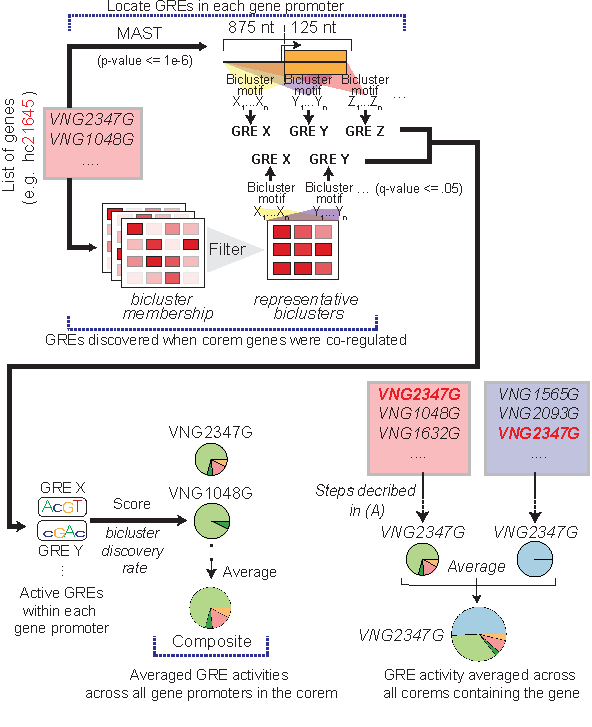
\includegraphics[width=0.7\linewidth]{figures/corem_gres.pdf}
\caption[Deciphering GREs responsible for regulating corems]{\textbf{Deciphering GREs responsible for regulating corems.} A GRE is implicated in regulation of a corem when it is both (1) located within an expanded region (-875nt to +125nt) around the translation start site of any gene in the corem; and (2) present in biclusters containing a large fraction of corem genes (top decile). Relative GRE influence is computed as the frequency with which each GRE was discovered in these representative biclusters (see Supplementary Methods for more details). Influence scores are illustrated as pie charts and reported for each gene individually (\eg, \textit{VNG2347G}); and as a composite by averaging across all genes in a corem. The width of each sector in the pie charts is proportional to the frequency of GRE discovery.}
\label{fig:corem_gres}
\end{figure}

\subsubsection{Detection of conditional operons}
\label{section:condop}
Condition-specific transcriptional isoforms of operons were predicted through corem membership. If any of the genes in an operon were found in a corem that did not contain all the other genes of the operon, we predicted that the operon had conditional isoforms. Operon annotations for both {\it H. salinarum} and {\it E. coli} were derived from \tmsamp{MicrobesOnline} \cite{alm_microbesonline_2005}. All predicted conditional operons, including the specific break sites and transcriptional isoforms is available on the website. The full list of validated predictions is provided in Table S7.
\subsubsection{Environmental ontology construction and usage}

We recorded a rich set of meta-data for all 1,495 experiments conducted with {\it H. salinarum} and used for construction of the \halo~ \egrine~model. The meta-data includes a detailed description of each experiment, including, for example: media composition, genetic background, concentration of perturbant, internal reference batch id, person who conducted the experiment, etc. We used this meta-information to classify experiments in an ontological framework, where two experiments can share specific meta-descriptions (\eg, $10^{-3}$ mol/L EDTA), or inherit more general relationships from the ontological structure (\eg, chemical perturbation). We used OBO-edit \cite{day-richter_obo-editontology_2007} to construct the ontology. The ontology contained 198 terms organized across three primary branches (environmental state, experimental state, and genetic state). The ontology flat file is available for download and meta-data annotations for every array in the dataset are available \href{http://egrin2.systemsbiology.net}{online}.

\begin{figure}[h!]
\centering
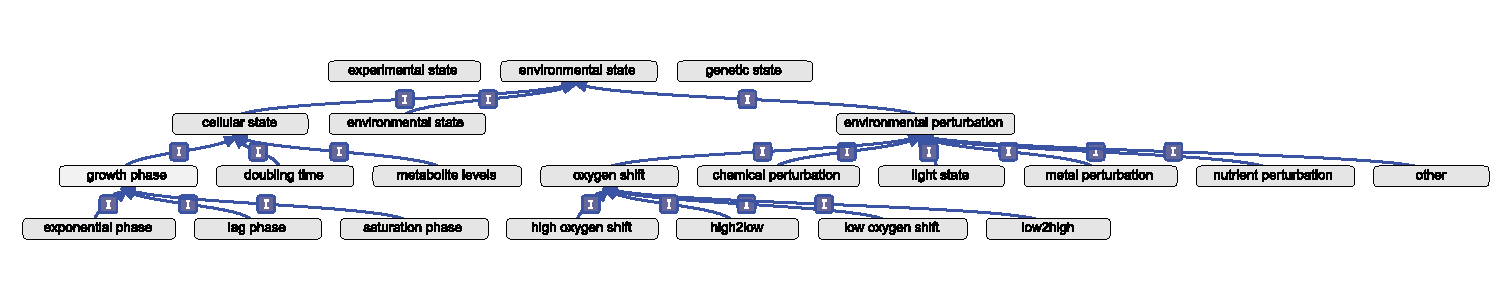
\includegraphics[width=0.95\linewidth]{figures/eo.pdf}
\caption[Environmental ontology hierarchically organizes relationships between experimental conditions from metadata collected across 1495 experiments in \textit{H. salinarum}]{{\bf Environmental ontology hierarchically organizes relationships between experimental conditions from metadata collected across 1495 experiments in \textit{H. salinarum}.} Subset of the environmental ontology constructed for \textit{H. salinarum} demonstrates many “is-a” (boxed ‘I’) relationships that organize similarities between descriptor terms descending from one of three root nodes (i.e., generic categorical descriptions). In this case a generic ontological term called `environmental state' gives rise to much more specific terms (e.g., exponential phase or high oxygen shift) that inherit (at the highest level) a relationship through their being related to the ‘environmental state’ of cells in the experiment. Each condition in the compendium is annotated with the most specific descriptors relevant to the experiment given metadata. The full environmental ontology is available for download from \href{http://egrin2.systemsbiology.net}{http://egrin2.systemsbiology.net}.}
\label{fig:eo}
\end{figure}

We used the ontology to classify enriched environmental features for GREs and corems. For corems, we used the set of conditions in which genes in the corem are significantly co-expressed (see Section \ref{section:rsd} above) to compute term enrichment using the \tmsamp{ontoCAT} \cite{kurbatova_ontocat:_2011}  \tmsamp{R}-package. Term enrichment was assessed statistically and reported as $q$-values using the hypergeometric test with Benjamini-Hochberg correction for multiple hypothesis testing.


\subsection{Global validation of GREs predicted by \egrine}
\label{section:tfbs:vs:regdb}

We compared the genome-wide locations of predicted GREs in the {\it E. coli} \egrine~model to experimentally mapped TF binding sites from \rdb~(BindingSiteSet table, filtered for experimental evidence and TFs with $\geq 3$ unique binding sites; a total of 88 TFs). We considered a GRE to be a significant match to a TF if a significant fraction ($q$-value $\leq 0.05$) of its predicted non-coding locations overlapped with the known binding locations for a particular TF (hypergeometric $p$-value $\leq 0.01$; see GRE definition in Section~\ref{section:gres}). In cases where a GRE significantly matched multiple TFs, only the most significant was reported.

We observed several instances where more than one GRE significantly matched the same TF. We were unable to determine whether this was the result of incomplete GRE clustering, ambiguities related to GRE scanning, limitations of the experimental data itself, or a reflection of subtle context-dependent variations in the binding preferences of these TFs. Since we did not observe clustering of GREs that map to the same TF upon re-clustering, we hypothesize that the observations may have biological origins, \ie, reflect condition-dependent variations in TF binding preferences that are the result, for example, of co-activator/repressor interaction or small molecule binding. It is interesting to note that TFs with the largest fraction of GRE matches include transcriptional dual regulators, such as FlhDC and UlaR (\ie, TFs with the ability to act as both activators and repressors). This is consistent with the observation that these TFs have context-dependent binding preferences. The complete set of validations, for both TFs and $\sigma$-factors, is listed in Table~S4.

\subsection{Global validation of regulatory interactions predicted by \egrine}
\label{section:aupr:vs:regdb}

We assessed the ability of the \egrine\ model to correctly infer known regulatory interactions using the \rdb\ database as a standard metric for comparison. Comparison to the \rdb\ gold-standard is common practice for evaluating model performance \cite{marbach_wisdom_2012}. We performed our evaluation with the version of \rdb~ used by the DREAM5 ensemble (based on \rdb\ release 6.8 \cite{marbach_wisdom_2012}) so that we could directly compare our results. The authors \cite{marbach_wisdom_2012} restricted the gold-standard to well-established interactions, annotated in \rdb\ with the `strong evidence' classification. In all cases, networks were integrated from predictions among the ensemble using an approach similar to that of \cite{marbach_wisdom_2012}, with subtle variations noted in each section, below. To facilitate a direct comparison, we reconstructed a new {\it E. coli} \egrine\ model using the same DREAM5 expression consortium as was used for the original DREAM5 competition (Section~\ref{section:dream5_data_compendium}). The predictions of this model were used {\it solely} for global validation and direct comparison with the DREAM5 community network, as described in this subsection.

We performed two global evaluations of the {\it E. coli} \egrine: (1) a comparison of the GREs detected in the model with experimentally mapped TF binding sites in \rdb~(Section~\ref{section:tfbs:vs:regdb}), and (2) a comparison of the predicted (TF $\rightarrow$ gene) regulation in \egrine~with the gene regulatory network from \cite{marbach_wisdom_2012}. For (2), we computed predicted regulatory networks from \egrine~in two ways: (a) direct (TF $\rightarrow$ target) predictions from \nwinf~ (Section~\ref{sec:nwinf_network}, and (b) a gene regulatory network derived from predicted GREs that were matched to TFs in \rdb~(Section~\ref{section:gre_grn_construction}). Construction of each of these networks is described in detail below (Section~\ref{sec:nwinf_network} and Section~\ref{section:gre_grn_construction}). The methods for, and results of the comparisons are described in Section~\ref{sec:network_comparisons}.

\subsubsection{Conversion of \egrine~\nwinf~influence predictions into a GRN}
\label{sec:nwinf_network}

We computed a direct (TF $\rightarrow$ gene) inferred {\it E. coli} gene regulatory network (GRN) from the \nwinf~predictions in the \egrine~ensemble. As with the original EGRIN model \cite{bonneau_predictive_2007}, \nwinf~influence predictions were originally made between the 296 putative {\it E. coli} TFs (Section \ref{section:eco_tfs}) and each of the $\sim 40,000$ biclusters in the ensemble. We then used a weighted average of the predicted influences among all networks in the ensemble, as follows. If \nwinf~predicted a (TF $\rightarrow$ bicluster) influence with weight $\beta$ then we added $\beta$ to a regulatory interaction between that TF and all genes in that bicluster. Weights $\beta$ were summed for each recurrence of the same (TF $\rightarrow$ gene) interaction. Note, we did not use $|\beta|$ in the individual sums, since we considered contradicting evidence to be cancelling rather than reinforcing. Finally, all (TF $\rightarrow$ gene) interactions in the final network were ranked by absolute total weight (here we {\it did} use $|\beta|$). As with the DREAM5 competition networks, the top 100,000 rankings were retained in the final network. The final \egrine~\nwinf~influence network is available \href{http://egrin2.systemsbiology.net/}{online}. 

\subsubsection{Conversion of \egrine~GRE detections into a predicted GRN}
\label{section:gre_grn_construction}

We computed a separate inferred {\it E. coli} gene regulatory network from predicted GREs in \egrine\ that were matched to TFs as described in Section~\ref{section:tfbs:vs:regdb}. We would like to stress that this inference relies upon (in this case, for {\it E. coli}) annotated binding sites for regulators, which could be statistically linked to predicted GREs through significant overlaps in their genomic locations. This enables inference of (TF $\rightarrow$ gene) direct influence predictions through the indirect relationship:

\begin{equation}
\label{eq:gre_network_relation}
\mathrm{TF} \overset{\mathrm{anno.}}{\rightarrow} \mathrm{GRE} \overset{\mathrm{pred.}}{\rightarrow} \mathrm{gene}.
\end{equation}

\noindent Thus for an understudied organism, such as {\it H. salinarum}, such a network of (TF $\rightarrow$ gene) influences could {\it not} be inferred; rather a (GRE $\rightarrow$ gene) interaction network would be the final product. Such a network still contains predictions which could be validated and acted upon, for example, for engineering purposes. A future direction of our research will be to statistically link TFs to predicted GREs, for example using direct GRN predictions such as those described above (\eg\ Section~\ref{sec:nwinf_network}, or \cite{marbach_wisdom_2012}).

(GRE $\rightarrow$ gene) predictions (in Eq.~\ref{eq:gre_network_relation}) were extracted from the \egrine\ model directly using the \MEME\ predictions for motif instances in the promoters of genes in each of the $\sim$40,000 \cm\ biclusters. We then used an unweighted average of the predictions among all bicluster in the ensemble, as follows. A (TF $\rightarrow$ gene) edge with a weight of 1 was added to the predicted network if the annotated binding sites for that TF could be matched with locations of a motif (Section \ref{section:tfbs:vs:regdb}), which was detected by \MEME\ in a bicluster in the promoter of the gene. Edge weights (1) were added for each additional prediction, in the ensemble of biclusters, of the same (TF $\rightarrow$ gene) interaction. As with the \nwinf~influence network (Section \ref{sec:nwinf_network}), the top 100,000 rankings were retained in the final network. The final \egrine~GRE-based network is available \href{http://egrin2.systemsbiology.net/}{online}. 

\subsubsection{Integration of predicted \egrine~\nwinf- and GRE-based GRNs}

Prior to integration of the two different predicted GRNs described above (Sections~\ref{sec:nwinf_network} and~\ref{section:gre_grn_construction}), we ensured that they were both equally represented in the integrated GRN by re-scaling their weights so that their sums would be equal. The GRNs were then combined into a single, integrated predicted \egrine\ GRN by simply summing the re-scaled weights for any edge predicted in both networks. Thus, this final network integration was a form of weighted average of the two (GRE and \nwinf) networks. This is {\it not} identical to the weighted rank average method described by \cite{marbach_wisdom_2012}, as it does not use a posteriori assessments of each network to assign their relative weights; rather the weights are simply adjust so that each network contributes equally to the predictions.

\subsubsection{Network comparisons and global performance assessments}
\label{sec:network_comparisons}

To compare \egrine\ performance to the DREAM5 ensemble, we computed standard precision-recall statistics for each network using the previously described DREAM5 gold standard GRN.  We computed area-under-the-precision-recall (AUPR) statistics to summarize the predictive performance. AUPR statistics were compared directly with the DREAM5 community ensemble network. By extension, the \egrine~AUPR performance can be compared to the individual best performers in DREAM5 as well (Figure~\ref{fig:egrin2:2:A} in \cite{marbach_wisdom_2012}). The results of these analyses are summarized in Figure~\ref{fig:egrin2:2:A} in the main text. We have made all network predictions available \href{http://egrin2.systemsbiology.net/}{online}. Complete precision-recall curves are shown in Figure~\ref{fig:pr_curves}. The curves are also available in tabular form \href{http://egrin2.systemsbiology.net/}{online}.

\begin{figure}[h!]
\centering
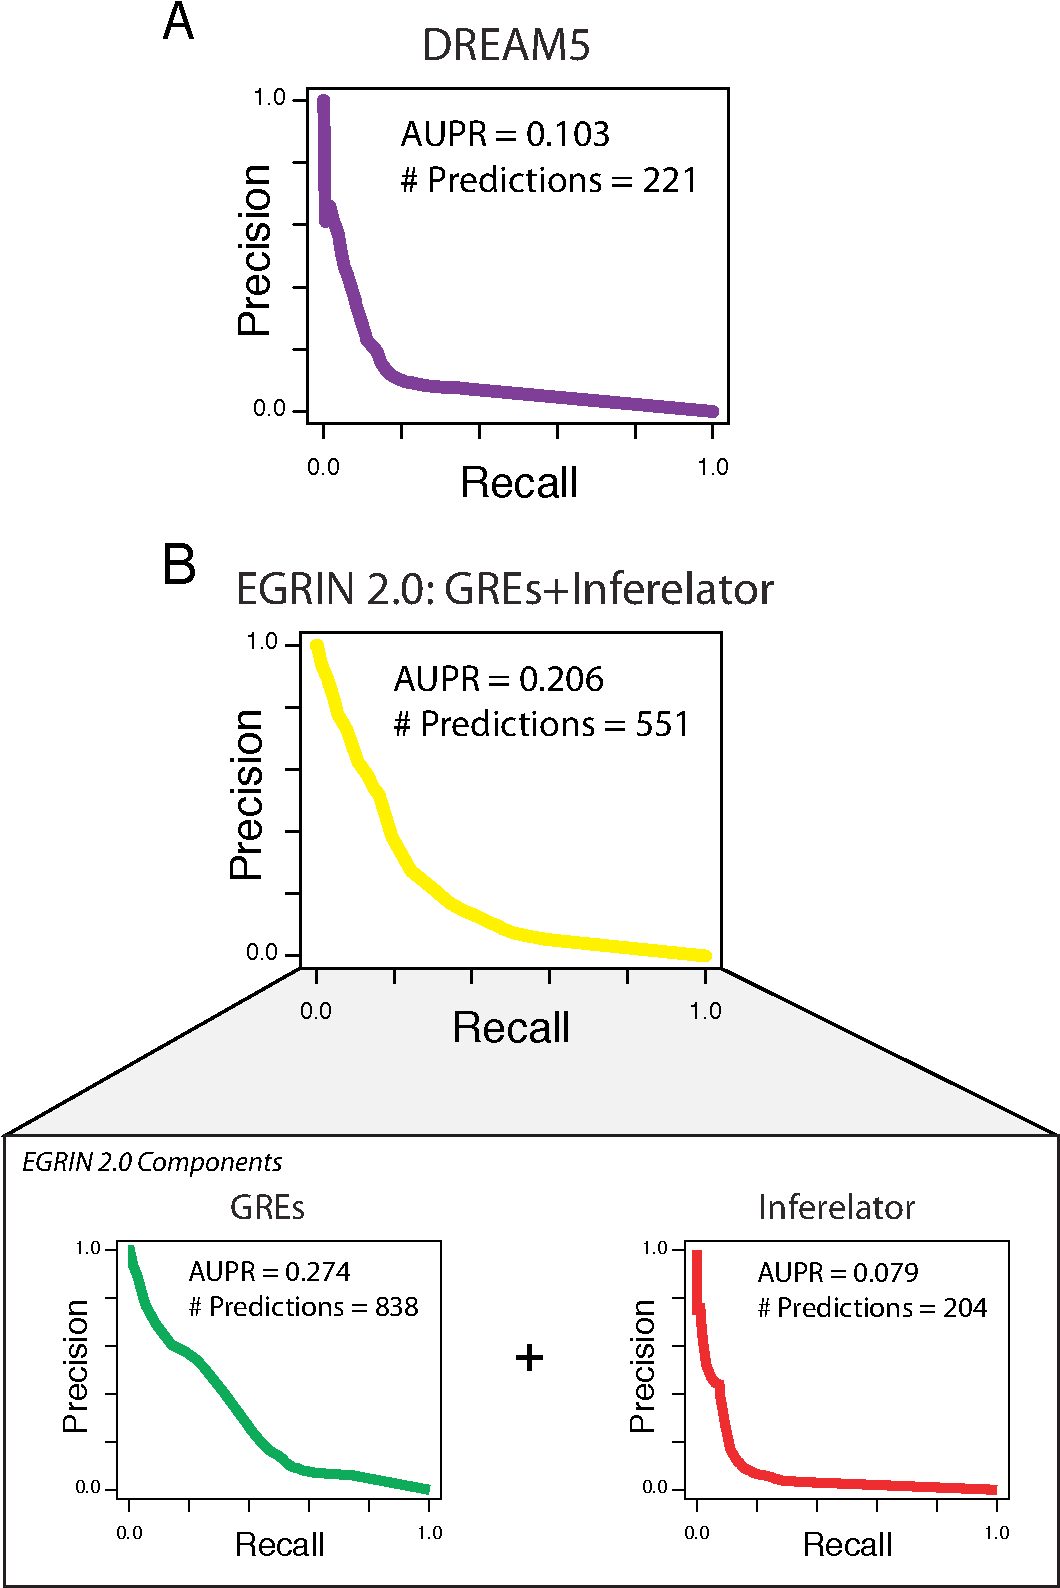
\includegraphics[width=0.5\linewidth]{figures/aupr.pdf}
\caption[Precision-recall performance for {\it E. coli} networks.]{\textbf{Precision-recall performance for \textit{E. coli} networks.} Comparison of precision-recall performance on {\it E. coli} \rdb~gold-standard (Section \ref{section:eco:gold:standard}), for the DREAM5 ensemble network (A), compared to \egrine (B).  We compare the GRE-based and \nwinf-based networks (bottom)to the integrated \egrine~network (top). The integrated \egrine~network consists of an equal weighting of the GRE-based and \nwinf-based networks.  The \egrine~networks were inferred using the DREAM5 mRNA expression compendium (Section \ref{section:dream5_data_compendium}). Area under the curve (AUPR) and the number of true-positive predictions at a precision of 25\% are listed for each curve.} 
\label{fig:pr_curves}
\end{figure}

We further investigated the convergence of the AUPR statistics for each of the \egrine-predicted regulatory networks as additional individual EGRIN models are added to the ensemble. This assessment helps to address the question of whether the approach utilized for ensemble integration has the desired property of performing better than most (if not all) of the individual models. Additionally, it can address the question of how many individual EGRIN models are necessary to achieve a given performance level. We observed that this is indeed the case for the \nwinf-based predictions extracted from the \egrine\ model (Figure~\ref{fig:cumulative_auprs}a), whose final AUPR of 8.5\% far exceeds the rather poor performance of all 106 individual component EGRIN models (with an average AUPR of 5.0\% and a maximum of 7.4\%). The performance of the ensemble for this measure converges rather quickly to the final measure, after roughly 50 of the 106 EGRIN models are integrated (taking into account the variance in models observed with integrating the models in different orders).  For the \egrine\ GRE-based predicted network (Figure~\ref{fig:cumulative_auprs}b), ensemble surpasses 84 (79\%) of the 106 individual component EGRIN models. This measure continues to improve until $\sim 80$ of the 106 models are integrated, suggesting that for this data set (the DREAM5 {\it E. coli} expression compendium), $\sim 100$ EGRIN models was a reasonable number to use in construction of the \egrine\ ensemble.

\begin{figure}[hp]
\centering
\mbox{
\subfigure[]{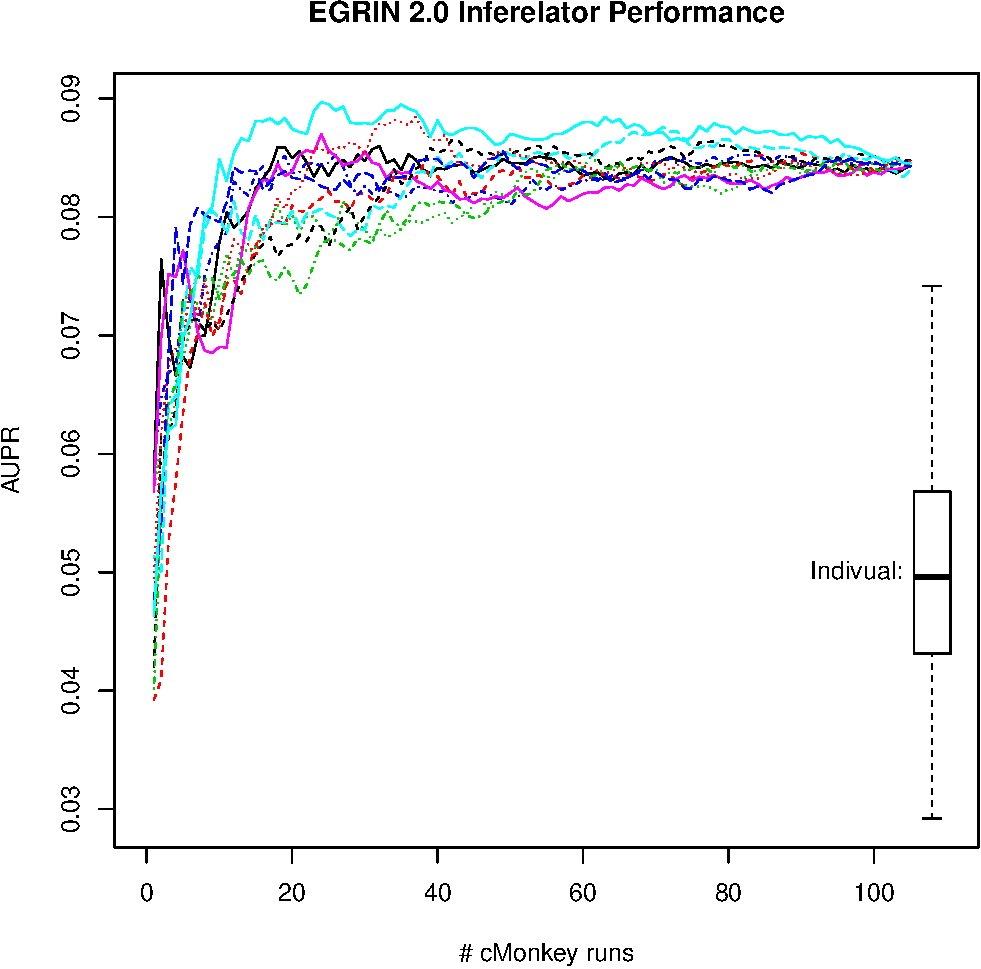
\includegraphics[width=0.4\linewidth]{figures/nwInf_cumulative_forPaper.pdf}}
\subfigure[]{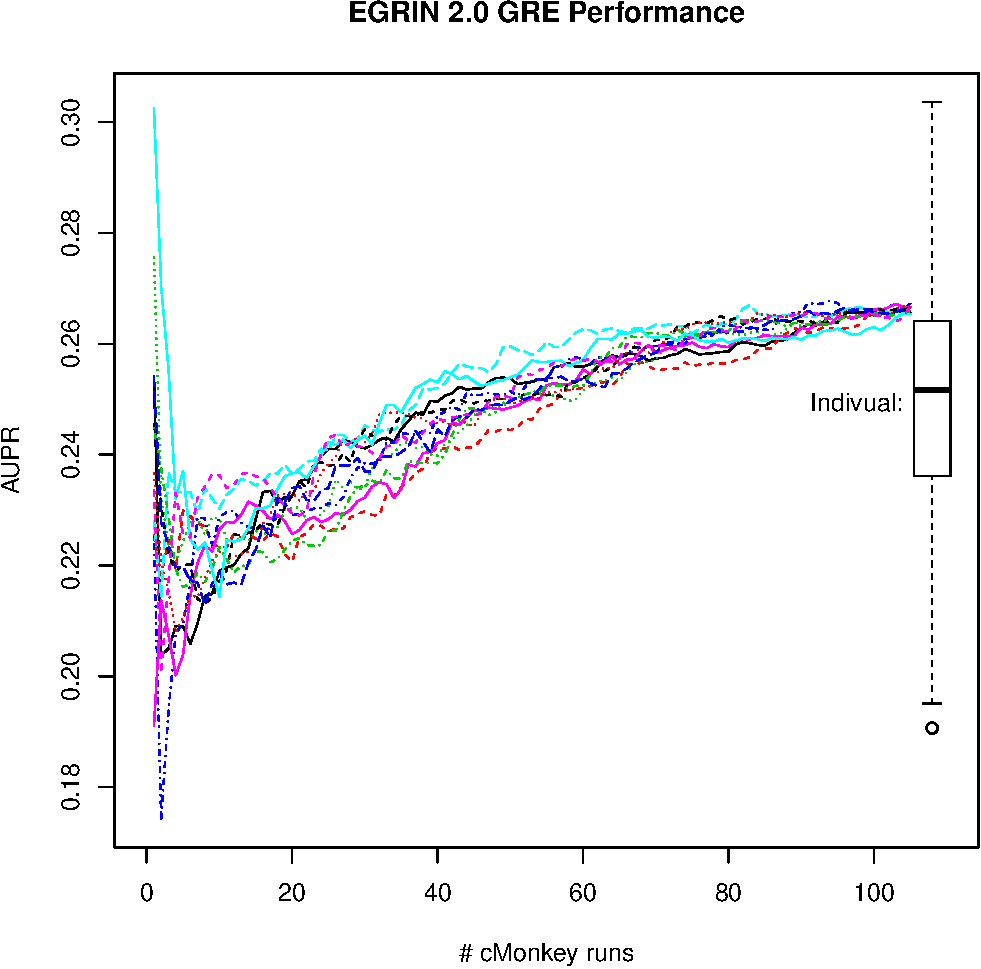
\includegraphics[width=0.4\linewidth]{figures/motif_cumulative_forPaper.pdf}}
}
\caption[Ensemble performance of individual GRN predictions]{\textbf{Ensemble performance of individual GRN predictions.} \egrine-inferred \textit{E. coli} regulatory network predictive performance (AUPR vs. {\it E. coli} DREAM5 \cite{marbach_wisdom_2012} gold standard) for \nwinf-based predictions (a) and GRE-based predictions (b) from \egrine. Shown for both networks is the cumulative AUPR as each of the 106 individual model components is integrated in to the ensemble (as described in Section~\ref{section:aupr:vs:regdb}). Lines showing the cumulative AUPR for randomized orderings of the components' integration into the ensemble reveal the slight variations in performance that could be observed, and that these converge prior to integration of the final ($106^{\text{\tiny th}}$) component. Also included for comparison is a box-whisker plot which shows the distribution of corresponding AUPR scores for the 106 individual EGRIN models. } 
\label{fig:cumulative_auprs}
\end{figure} 

Figure \ref{fig:argR_purR_networks} shows the inferred networks for two genes regulated by PurR and ArgR (comparing predictions from \egrine, \tmsamp{CLR}, DREAM5, and \tmsamp{RegPrecise} to the annotations in \rdb). The result demonstrates that GRE-based approaches can discover interactions that are not predicted using direct approaches (See Section~\ref{section:gre_grn_construction}).

\begin{figure}[hp]
\centering
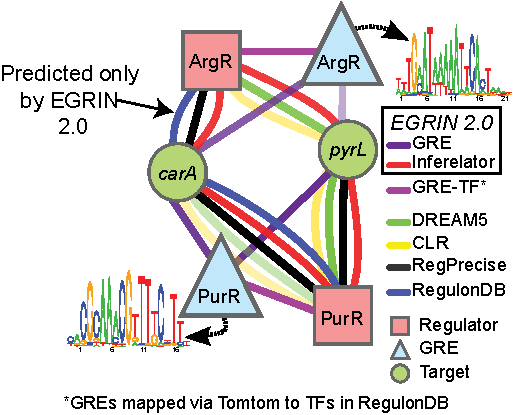
\includegraphics[width=0.5\linewidth]{figures/argR_purR_networks.pdf}
\caption[Integration of GRE discovery and \nwinf\ predictions yields comprehensive and detailed gene regulatory networks]{\textbf{Integration of GRE discovery and \nwinf\ predictions yields comprehensive and detailed gene regulatory networks.} \egrine-inferred \textit{E. coli} regulatory subnetwork for two genes (green circles) in the PurR/ArgR regulon: \textit{carA} (\textit{b0032}) and \textit{pyrL} (\textit{b4246}). The \egrine~predictions are divided into GRE-based (dark violet) and \nwinf-based (red), and compared to predictions (or annotations) from other algorithms/databases (yellow: \tmsamp{CLR}; green: DREAM5 ensemble; black: \tmsamp{RegPrecise}; blue: \tmsamp{RegulonDB}). In two cases (ArgR$\rightarrow$carA and ArgR$\rightarrow$pyrL), \egrine~discovers regulatory interactions that were missed by either hand-curated databases or expression-based inference procedures.} 
\label{fig:argR_purR_networks}
\end{figure} 

\subsection{Validation of condition-specific operon isoforms by tiling array transcriptome measurements}

We validated the prevalence of multiple, condition-specific transcriptional isoforms from operons in \eco\ by measuring changes in the transcriptome across growth, from lag-phase (OD600 = 0.05) to late stationary phase (OD600 = 7.3). The experimental platform and other experimental details are described in Section \ref{section:ecoarray}. We used multivariate recursive partitioning, including signals from both relative changes in expression along the growth curve, as well as raw RNA hybridization signal to call putative transcription breaks as previously described \cite{koide_prevalence_2009}. To determine the significance of our finding, we computed a $p$-value describing the significance of the overlap between our predictions (see Section \ref{section:condop}) and the experimental observations using the cumulative hypergeometric distribution.

Figures \ref{fig:dpp_ecoli_expression}, \ref{fig:galE}, and \ref{fig:ptsh} below depict several operons annotated with condition-specific transcriptional isoforms. We have integrated GRE elements discovered near break sites with the transcriptional measurements.

\begin{figure}[hp]
\centering
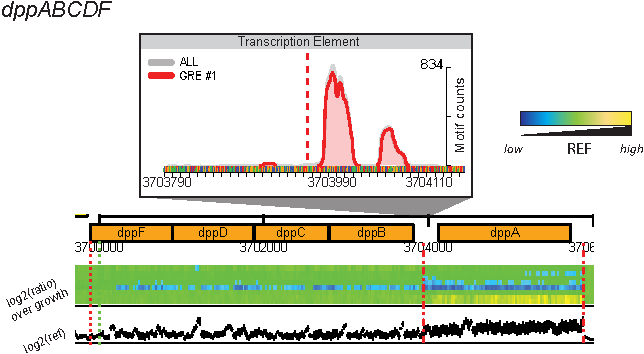
\includegraphics[width=0.7\linewidth]{figures/dpp_ecoli_expression.pdf}
\caption[GREs regulate multiple transcript isoforms from operons in {\it E. coli}, \textit{dppABCDF}]{\textbf{GREs regulate multiple transcript isoforms from operons in {\it E. coli}, \textit{dppABCDF}.} GREs coincide with experimentally measured break sites. Three examples of experimentally determined transcription break sites (red dashed lines) in operons predicted by corems to be conditionally segmented. Expression levels of these regions were profiled across growth in rich media (heatmap). Inset contains region immediately surrounding a transcriptional break site, including counts of GREs discovered at these locations.} 
\label{fig:dpp_ecoli_expression}
\end{figure}

\begin{figure}[hp]
\centering
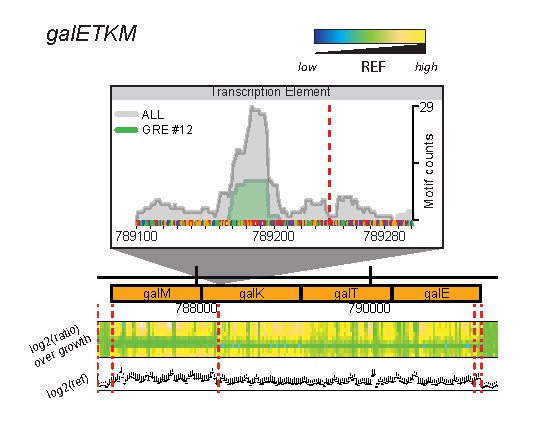
\includegraphics[width=0.7\linewidth]{figures/galE.pdf}
\caption[GREs regulate multiple transcript isoforms from operons in
  {\it E. coli}, \textit{galETKM}]{\textbf{GREs regulate multiple
    transcript isoforms from operons in {\it E. coli},
    \textit{galETKM}.} Caption details included in Figure
  \ref{fig:dpp_ecoli_expression}}
\label{fig:galE}
\end{figure}

\begin{figure}[hp]
\centering
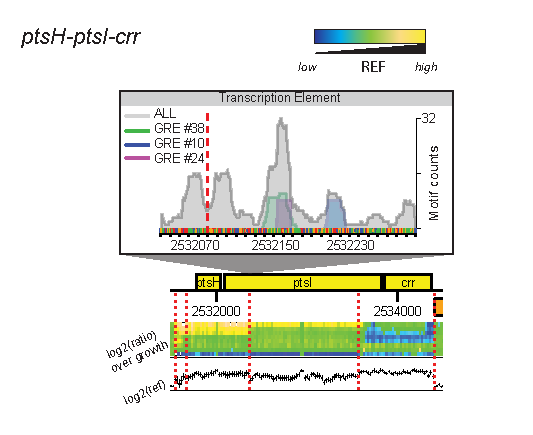
\includegraphics[width=0.7\linewidth]{figures/ptsh.pdf}
\caption[GREs regulate multiple transcript isoforms from operons in
  {\it E. coli}, \textit{ptsH-ptsI-crr}]{\textbf{GREs regulate
    multiple transcript isoforms from operons in {\it E. coli},
    \textit{ptsH-ptsI-crr}.} Caption details included in Figure
  \ref{fig:dpp_ecoli_expression}.}
\label{fig:ptsh}
\end{figure}

\subsection{Gene-gene co-fitness correlations in corems}

To assess the phenotypic consequences of co-regulation in corems, we assessed whether genes grouped into corems had significantly similar fitness consequences in many environments (\ie, the effect of deleting one gene is highly similar to the effect of deleting the other across many environments). We used the high-throughput fitness screen described in Section \ref{section:fitness} to quantify these relationships.

We compared the enrichment for high co-fitness relationships in corems to other ways of assigning co-regulatory modules, including regulons (\tmsamp{RegPrecise}, \rdb), operons, and \tmsamp{WGCNA}. The gene modules for regulons (annotated in \rdb\ or \tmsamp{RegPrecise} \cite{novichkov_regprecise_2012}) consisted of genes annotated to a common TF. For WGCNA, we assigned modules using the same community detection procedures that we used to define corems from the \egrine~ensemble (See \ref{section:gBg}). The gene co-expression modules were computed from the weighted \tmsamp{WGCNA} adjacency matrix.

For the results presented in Figure~\ref{fig:egrin2:2:B}, we compared the distributions of Pearson correlations between relative changes in fitness across pairs of genes within each module, using the one-tailed Kolmogorov-Smirnov test (KS-test). We report the KS $D$-statistic. The precision/recall characteristics for each model are contained in Table~S5.

We extended this analysis by investigating whether the enriched high co-fitness gene-gene relationships in corems consist of relationships that could be described fully by regulons or operons. To answer this question, we removed all gene pairs from corems that are also present in operons or regulons and computed the KS-test again (Figure \ref{fig:fitness_wo_operons}). We still observe a significant number of high co-fitness relationships, suggesting that corems capture physiologically meaningful co-regulatory relationships between genes that cannot be explained by existing paradigms.

\begin{figure}[hp]
\centering
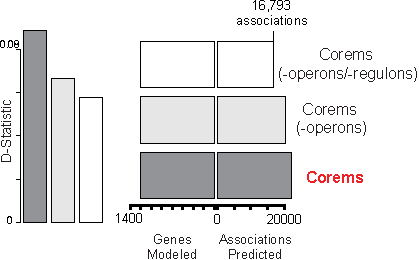
\includegraphics[width=0.6\linewidth]{figures/fitness_wo_operons.pdf}
\caption[\egrine~models highly correlated co-fitness relationships that cannot be explained by operons or regulons]{\textbf{\egrine~models highly correlated co-fitness relationships that cannot be explained by operons or regulons.} (Left) Enrichment for highly correlated, pairwise fitness measurements in gene knock outs across 324 conditions before and after removing gene associations annotated by operons (Microbes Online) and regulons (RegulonDB and RegPrecise) (KS-test,$D$-statistic). Two-thirds of gene-pairs with most highly correlated fitness within corems are not annotated by operons or regulons. (Right) Number of genes and associations predicted.} 
\label{fig:fitness_wo_operons}
\end{figure}



 

 
 
    % ========== Chapter 3
 
\chapter {\uppercase{A systems-level model of the microbial regulatory genome}}
\label{chap:3}

 Microbes can tailor transcriptional responses to diverse environmental challenges despite having streamlined genomes and a limited number of regulators. Here, we present data-driven models that capture the dynamic interplay of the environment and genome-encoded regulatory programs of two types of prokaryotes: \eco (a bacterium) and \halo (an archaeon). The models reveal how the genome-wide distributions of \textit{cis}-acting gene regulatory elements and the conditional influences of transcription factors at each of those elements encode programs for eliciting a wide array of environment-specific responses. We demonstrate how these programs partition transcriptional regulation of genes within regulons and operons to re-organize gene-gene functional associations in each environment. The models capture fitness-relevant co-regulation by different transcriptional control mechanisms acting across the entire genome, to define a generalized, system-level organizing principle for prokaryotic gene regulatory networks that goes well beyond existing paradigms of gene regulation.\\


 \noindent This chapter has been modified from:\\

\noindent Brooks AN$^{*}$, Reiss DJ$^{*}$, Allard A, Wu W, Salvanha DM, Plaisier CL, Chandrasekaran S, Pan M, Kaur A, Baliga NS. (2014) A system-level model for the microbial regulatory genome. \emph{Mol Syst Biol.}  10: 740.\\

 \noindent * Indicates equal contribution 

\paragraph{Chapter Highlights}

\begin{itemize}
\item Method to infer a genome-wide map of gene regulatory elements (GREs) and their 
condition-specific activities directly from genome sequence and transcriptome profiles
\item Novel co-regulatory structure, the \textbf{corem}, describes condition-specific partitioning 
and reorganization of operons and regulons by combinatorial and other nuanced regulatory mechanisms
\item Corems group together functionally related genes that have tight co-expression in 
some but not all environments
\item Corems associate genes from different operons and regulons that have highly similar 
fitness consequences
\end{itemize}


\section{Summary}
 
Genome-scale reconstruction of gene regulatory networks for two diverse microbial species using genome sequence and transcriptional profiles reveals complex, condition-dependent co-regulated modules (corems) and \textit{cis}-regulatory mechanisms that generate them. 

\section{Introduction}

Deciphering how microbes colonize dynamically changing environmental niches with few regulators and streamlined genomes will require mechanistic and system-level characterization of their gene regulatory networks (GRNs). Even a streamlined microbial genome encodes an intricate network of regulatory and signaling systems that sense and process extracellular and intracellular information to regulate gene expression at multiple levels (transcriptional, post-transcriptional, translational, allosteric, etc.). A significant fraction of these environmental signals are relayed by transcription factors (TFs) that modulate transcriptional activity when they bind DNA. TFs typically bind conserved, $\sim$6-20 nucleotide DNA sequences located in intergenic regions immediately adjacent to transcription initiation sites. These TF binding sites are referred to as gene regulatory elements (GREs). 

A goal of systems biology has been to map the complete set of TFs, GREs, and their interactions, using high throughput techniques including ChIP-chip \cite{blat_cohesins_1999}, yeast two-hybrid \cite{fields_novel_1989}, DNase I hypersensitivity \cite{crawford_identifying_2004}, or more modern variants using sequencing \cite{johnson_genome-wide_2007}. In parallel, attempts have been made to infer GRNs directly from gene expression data \cite{bonneau_predictive_2007,de_smet_advantages_2010,faith_large-scale_2007,segal_genome-wide_2003}. Such high throughput approaches are attractive because they would accelerate discovery in understudied organisms by circumventing significant labor and cost.

Inference of systems-scale GRNs that are both predictive and mechanistically accurate, however, has proven difficult for a number of reasons, including: (1) the statistical challenge of confidently discovering GREs across the genome, \textit{de novo}; (2) the consequences of non-linear gene regulatory dynamics, including combinatorial molecular interactions at gene promoters; and (3) the often non-canonical locations of GREs throughout the genome (including internal to operons and within coding sequences). A remaining challenge, therefore, is to produce an unbiased map of TF-binding site locations throughout the genome, including information about what binds to those sequences, in what contexts they are bound, and, importantly, how TF-binding throughout the genome ultimately influences cellular physiology.     

We previously constructed an ‘Environment and Gene Regulatory Influence Network’ (EGRIN) for \halo \cite{bonneau_predictive_2007}. This model was constructed in two steps. First, modular organization of gene regulation was deciphered through semi-supervised biclustering of gene expression, guided by biologically informative priors and \textit{de novo cis}-regulatory GRE detection for module assignment (cMonkey; \cite{reiss_integrated_2006}). Second, using a regression-based approach transcriptional changes of genes within each bicluster were modeled as a linear combination of influences of TFs and environmental factors (Inferelator; \cite{bonneau_inferelator:_2006}). 

The EGRIN networks learned by cMonkey and Inferelator accurately predicted transcriptional changes in new environments, a feat that has subsequently been replicated by other network inference strategies \cite{faith_large-scale_2007,lemmens_distiller:_2009,marbach_wisdom_2012}; yet, these network models have failed to capture detailed regulatory mechanisms that operate only in specific environments, at non-canonical genomic locations, or in complex combinatorial schemes. 

Here, we report significant advancement to inference of GRNs that overcomes many of these challenges. We have developed a methodology applicable to any sequenced microbe in culture to infer \egrine~models for two representative organisms from the primary branches of prokaryotic life - bacteria and archaea: (1) \eco, a bacterium with a wealth of information about transcriptional regulatory mechanisms and related experimental data \cite{salgado_regulondb_2006}; and (2) \halo, an archaeon with few examples of regulatory mechanisms that have been characterized in detail, but extensive experimental data from recently conducted systems biology studies \cite{bonneau_predictive_2007,koide_prevalence_2009}. The wide range of prior knowledge for these organisms proved invaluable for testing our model. In addition, we have also conducted new experiments that validate \egrine~predicted complex modulation of the \eco transcriptome structure during varying stages of growth in rich media. 

\egrine~models the organization of GREs within every promoter, their distributions across the entire genome – even in non-canonical locations – and links the contexts in which they act to conditional co-regulation of genes. These features are formalized in \egrine~by condition-specific, co-regulated modules or corems.  Corems are overlapping sets of co-regulated genes that, in some cases, group together genes from different regulons and, in other cases, subdivide genes of the same regulon, or even the same operon. \egrine~formalizes how the genome-wide coordination of previously characterized and newly discovered regulatory mechanisms dynamically associates genes into corems, bringing together functionally-related genes from different operons and regulons whose deletions have similar impact on cellular fitness. Our results show how prokaryotes, much like eukaryotes, can produce complex gene expression patterns with a relatively small number of regulatory components.  

\section{Results}

\subsection{Construction of \egrine} 

We developed an ensemble-framework that models the condition-specific global transcriptional state of the cell as a function of combinations of transient TF-based control mechanisms acting at intergenic and intragenic promoters across the entire genome. Specifically, for each of the two orgainsms, \halo and \eco, we aggregated associations across genes, GREs, and environments from many individual EGRIN models, each trained on a subset of the gene expression data, to (1) quantify confidence in each model-predicted association; (2) reveal context-dependent regulatory mechanisms that occur infrequently in the data; and (3) discover non-canonical regulatory mechanisms. We refer to the aggregated, post-processed ensemble of EGRIN models as \egrine, and conditionally co-regulated modules as corems (details provided in Chapter \ref{chap:2}, Figure \ref{fig:egrin2:1}; ensemble statistics available in Table \ref{tab:stats}). 

\begin{figure}[h!]
    \centering
    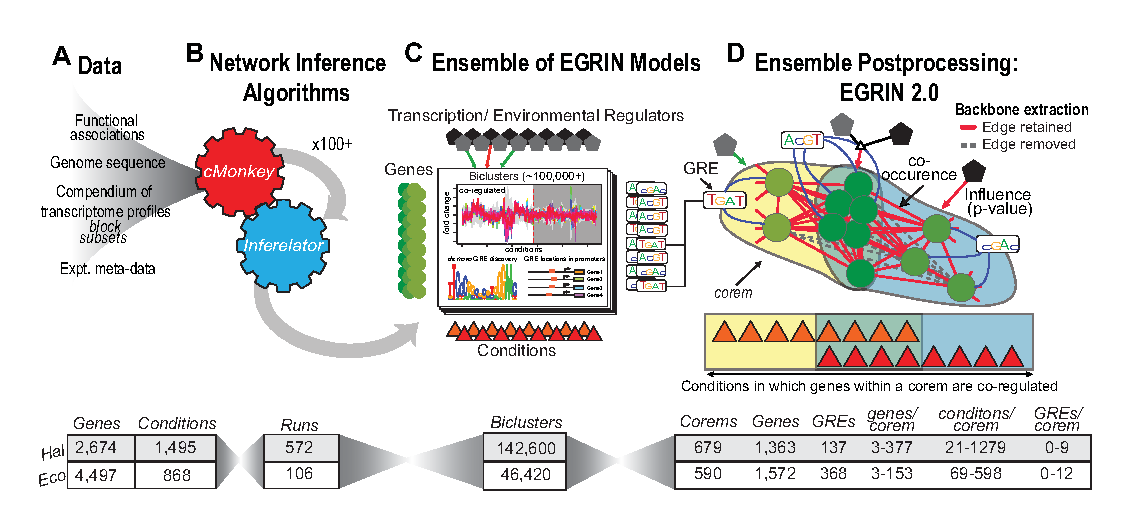
\includegraphics[width=0.9\textwidth]{figures/egrin2_fig1}
 	\caption[\egrine~Model Construction.]{\egrine~Model Construction. Workflow summary for \egrine. Tables below each panel contain detailed statistics for the \halo and \eco models. (A) and (B). The cMonkey and Inferelator algorithms were applied many times to subsets of gene expression data from large compendiums of transcriptome profiles to construct many individual EGRIN models.(C) Individual EGRIN models were integrated into an ensemble for filtering, querying, and ranking relationships among genes (circles), regulators (hexagons), motifs (sequence logos), and the conditions (triangles) in which these relationships were discovered.(D) The library of relationships was mined using algorithms for motif clustering, backbone extraction, and community detection to construct the final \egrine~model. In \egrine, overlapping co-regulated sets of genes (corems, shaded regions of the graph) are statistically associated with specific gene regulatory elements (GREs, sequence logos, blue edges), regulatory influences (pentagons, green or red depending on direction), and environments in which they are co-regulated (triangles). Each node represents a gene in the model. Genes are connected via co-regulation edges, with weights that reflect the number of occurrences in the ensemble. Dashed edges were removed from the model by backbone extraction.}
    \label{fig:egrin2:1}
\end{figure}

\subsection{\egrine~discovers experimentally characterized regulatory mechanisms}

A high quality GRN has to be both comprehensive (high recall) and accurate (high precision). To evaluate the quality of \egrine, we compared its predictions on \eco to RegulonDB \cite{gama-castro_regulondb_2011}, an extensive, manually-curated, gold-standard of experimentally validated TF-gene interactions. We compared the genome-wide distribution of each \textit{de novo} discovered GRE in \egrine~to experimentally characterized binding locations of every TF in RegulonDB. This comparison showed that \egrine~had accurately located binding sites for 60\% of experimentally characterized TFs in RegulonDB (53 out of 88 at FDR $\leq$ 0.05 for all TFs with $\geq$3 unique sites; see Chapter \ref{chap:2}). At a standard precision cutoff of 25\%, \egrine~recovered 577 ``strong evidence'' TF-gene interactions, which is 2.7X as many validated interactions as algorithms that exclusively use expression data, i.e. without genomic sequence information (Figure \ref{fig:egrin2:2:A}, Figure \ref{fig:pr_curves}, Figure \ref{fig:cumulative_auprs}, Figure \ref{fig:argR_purR_networks}, Table S4, \ref{chap:2}; \cite{faith_large-scale_2007,marbach_wisdom_2012}. As expected, the ensemble network had greater precision and recall than individual cMonkey runs. Furthermore, integration of Inferelator-predicted TF influences with GRE-based predictions increased overall algorithm performance. These results show that integrating complementary methods, such as regression-based inference of TF regulation, biclustering-based inference of network modularity, and \textit{de novo} GRE detection, improves the accuracy and coverage of the inferred GRN. 

\begin{figure}[h!]
    \centering
    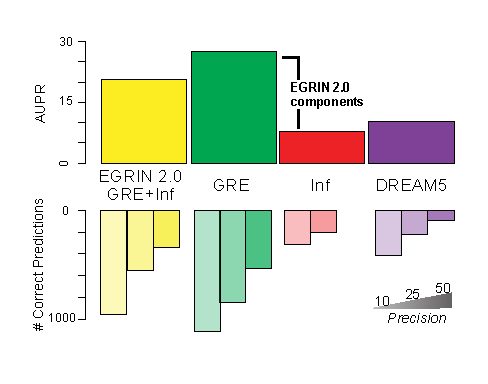
\includegraphics[width=0.75\textwidth]{figures/egrin2_AUPR}
 	\caption[\egrine~Model Validation: Performance on RegulonDB]{\egrine~performance on experimentally-validated gold-standard network. Comparison of \egrine~model components (“GRE”: GRE-only; “Inf”: Inferelator-only) to the DREAM5 community ensemble network, against RegulonDB (strong evidence code). (Top) Area under the precision-recall curve (AUPR) and (Bottom) number of correct predictions at 10, 25, and 50\% precision. 
}
    \label{fig:egrin2:2:A}
\end{figure}

Since few GREs have been characterized in \halo, we performed a global assessment and discovered that GREs in \egrine~occur at consistent locations across many gene promoters throughout the genome (Figure \ref{fig:gre_global_locs_hal}). We could even assign putative roles for some GREs based on their location relative to transcription start sites (TSSs). For instance, the location of TATA box-like elements (GRE \#25) between -21 to -40 nucleotides upstream of TSSs in \halo is consistent with the characterized location of basal elements in archaeal promoters (TFB/TBP complex recognition sites) \cite{geiduschek_archaeal_2005}. Similarly, other elements occurred either consistently downstream of the TATA box (putative repressors, e.g. GRE \#1 and \#2) or upstream of these basal elements (putative activators, e.g. GRE \#5). Thus, even in organisms where genome-wide TF binding data are scarce, \egrine~can be used to infer and predict putative roles for \textit{de novo} discovered GREs.

\subsection{Corems model genes with similar effects on organismal fitness}

We investigated whether the model goes beyond simple co-expression to group together genes that have similar phenotypic contributions. We did this because previous studies have reported weak correlation between gene expression and fitness \cite{price_indirect_2013}. For all genes in each corem, we computed pairwise correlations of fitness effects in a dataset generated from a survey of relative growth rates for 3,902 single gene deletion strains of \eco subjected to a chemical genomics screen spanning 324 different environmental conditions \cite{nichols_phenotypic_2011}. We discovered that more than one-third of gene-pairs with the most similar fitness effects across environments (Pearson correlation $>$ 0.75) were grouped together in corems. We evaluated significance of this result by performing similar analysis using modules based-on co-expression (WGCNA; \cite{langfelder_wgcna:_2008}), and regulons (RegPrecise and RegulonDB), where a regulon is defined as a set of genes regulated by the same TF. While WGCNA and regulons also grouped significant numbers of high fitness-correlated gene-pairs (one-sided KS-test $<$ 0.05), corems were more enriched for highly similar fitness associations (higher KS D-statistic) and in general provided greater precision and coverage (Figure \ref{fig:egrin2:2:B}). As an example, corems group together 5X as many gene-pairs with highly correlated fitness effects as RegPrecise, RegulonDB, or WGCNA (134 out of 185 gene-pairs with Pearson correlation ≥0.9 are discovered in corems, Table S5). Most important, corems retained a high degree of enrichment for gene-pairs with highly correlated fitness effects after removing all associations attributable to operon and regulon memberships, and even combinatorial control (Figure \ref{fig:fitness_wo_operons}, Table S5\footnote{All tables available in \cite{brooks_systemlevel_2014} and \href{http://egrin2.systemsbiology.net}{online}}). This suggested that corems model regulatory associations among genes that cannot be explained within the existing paradigms of regulons and operons. 

\begin{figure}[h!]
    \centering
    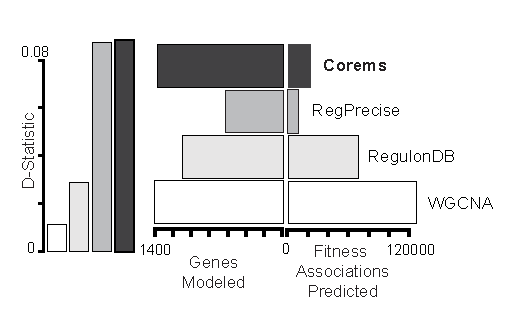
\includegraphics[width=0.75\textwidth]{figures/egrin2_corem_fitness}
 	\caption[\egrine~Model Validation: Fitness contributions]{Enrichment of similar fitness effects within gene modules. (Left) Magnitude of enrichment for gene pairs with similar fitness consequences, assessed by one-tailed KS-test (KS D-statistic). (Right) Number of genes and gene-pairs predicted by each method.  Comparison methods include \egrine~corems, co-expression modules from WGCNA, and regulons from databases (RegPrecise and RegulonDB). 
}
    \label{fig:egrin2:2:B}
\end{figure}

In other words, corems group together genes that are regulated by distinct TFs. For example, the ArgR-regulated acetylglutamate kinase, \textit{argB}, and \textit{ilvC}, an IlvY-regulated ketol-acid reductoisomerase have fitness correlation of 0.95 (Pearson coefficient), which suggests an important coupling between branched-chain amino acid biosynthesis and arginine metabolism (Table \ref{tab:table1}). Although these genes are regulated by distinct TFs (ArgR and IlvY, respectively), the high similarity of their expression changes across multiple environments brings them together into the same corem (ec512157). There are 319 highly correlated (Pearson correlation $\geq$ 0.75) fitness associations among genes from different regulons that are modeled by corems – each of which suggests an important physiological coupling that results from the coordinated activity of TFs (Table E6). These examples illustrate how the organizing principle of corems captures fitness-relevant associations within a GRN that are overlooked by current definitions for gene-gene co-regulation, such as regulon and operon.

\subsection{\egrine~predicts detailed organization and context-specific importance of GREs in gene promoters}

We next investigated accuracy of \egrine~predicted spatial organization of GREs, and their context-specific roles in mediating transcriptional regulation from specific promoters. We did this analysis in context of one of the best studied \halo promoters: \textit{kdpFABC}, with data not used for model training. The \textit{kdp} operon encodes an ATP-dependent potassium transporter that counterbalances extremely high salinity in the extracellular environment. \egrine~predicts that at least three GREs are putatively responsible for mediating transcriptional regulation of this operon: GRE \#1, GRE \#148, and GRE \#106 (Figure \ref{fig:egrin2:2:C}). The locations of these GREs align to regions that were experimentally characterized in an independent study as “Operator” and “BRE-TATA” elements, respectively. This demonstrates that \egrine~is able to accurately predict the organization of GREs in gene promoters at nucleotide-resolution.

\begin{figure}[h!]
    \centering
    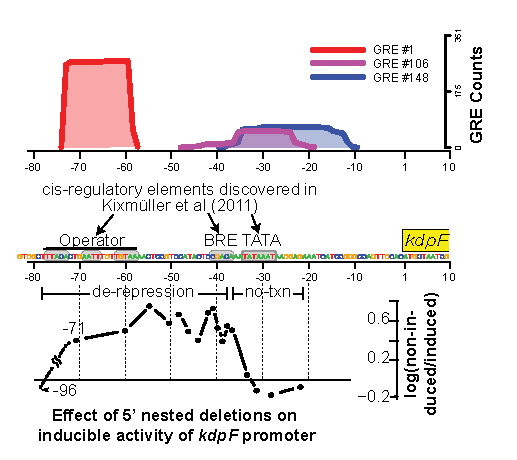
\includegraphics[width=0.75\textwidth]{figures/egrin2_kdpvalidaton}
 	\caption[\egrine~Model Validation: Regulatory elements of \textit{kdp} operon, \halo]{Promoter architecture of the \halo \textit{kdpFABC} promoter predicted by the \egrine~model. (Top) Frequency of GRE alignment to each position in the \textit{kdpFABC} promoter. GREs are indicated by shaded lines. (Middle) Genome sequence marked with putative functions by \cite{kixmller_archaeal_2011}. (Bottom) Transcriptional activity measurements from truncated promoters used by authors to validate these sites. 
}
    \label{fig:egrin2:2:C}
\end{figure}

Since these sites also had characterized transcriptional roles [determined by promoter truncation experiments \cite{kixmller_archaeal_2011}], we asked whether \egrine~would have been able to predict these roles given the context in which the GREs were discovered. Strikingly, we find that GRE \#1 (aligned to the “Operator”) was discovered in environments, including low salt (hypergeometric FDR = $6.9\times10^{-12}$), where the transcript is repressed (one-sided t-test pval = 0.048), while GRE \#106, which aligns to the “BRE-TATA” region, was discovered in environments, including low oxygen (hypergeometric FDR = $1.8\times10^{-9}$), where transcript levels are elevated (one-sided t-test pval = $1.2\times10^{-3}$; \ref{chap:2}). Here onwards, we will refer to a GRE as ``active'' when it is predicted to be important for transcriptional regulation at a specific promoter (see Figure \ref{fig:corem_gres} for details). The environmental contexts in which the three GREs in the \textit{kdp} promoter are predicted to be active are especially interesting because perturbations to external potassium levels and energy-producing mechanisms have been shown to significantly influence expression of this operon \cite{wurtmann_evolutionarily_2014}. Thus, \egrine~had accurately predicted that a trade-off in relative influence of GRE \#1 (repressing) versus GRE\#106 (activating) controls expression levels of this operon in a condition-specific manner, exactly as was characterized by independently performed experiments. This is powerful because it shows that using \egrine~we can predict when (context) and how (activate or repress) a specific GRE(s) within a promoter might act, even though we might not know the precise regulatory mechanism (e.g., TF binding/unbinding, allosteric activation, co-factor interaction, etc).

\subsection{Conditionally active GREs within each promoter reorganize gene memberships within corems}

We investigated whether \egrine~accurately links the same GRE at different promoter locations, the environments in which it is predicted to be active within each of those promoters, and conditional co-regulation of the associated genes (see \ref{chap:2}). We did this analysis with genes of nucleotide biosynthesis in \eco, including key branch-point enzymes \textit{carA} (\textit{b0032}) and \textit{pyrL} (\textit{b4246}), since they are canonical, extremely well studied pathways that are critical for survival. Regulation of \textit{carA}, which catalyzes synthesis of an important metabolic intermediate in several amino acid and nucleotide metabolism pathways (carbamoyl phosphate), is known to be sensitive to purine and pyrimidine pools, as well as arginine \cite{neidhardt_escherichia_1996}. \egrine~discovered several previously characterized and new mechanisms for regulation of carA, including two GREs (GRE \#4 and GRE \#12) that match to consensus sequence motifs for PurR and ArgR, respectively \cite{piette_dna_1984} (Figure \ref{fig:egrin2:2:D}). Remarkably, \egrine~discovered novel overlapping organization of GRE \#4 and GRE \#12 in the \textit{pyrL} promoter that was not previously reported in RegulonDB (Figure \ref{fig:pyrL}). This promoter organization was verified upon mapping overlapping binding sites for ArgR and PurR precisely at the predicted locations in ChIP-chip data that were not used in model training \cite{cho_deciphering_2012,cho_purr_2011}.

\begin{figure}[h!]
    \centering
    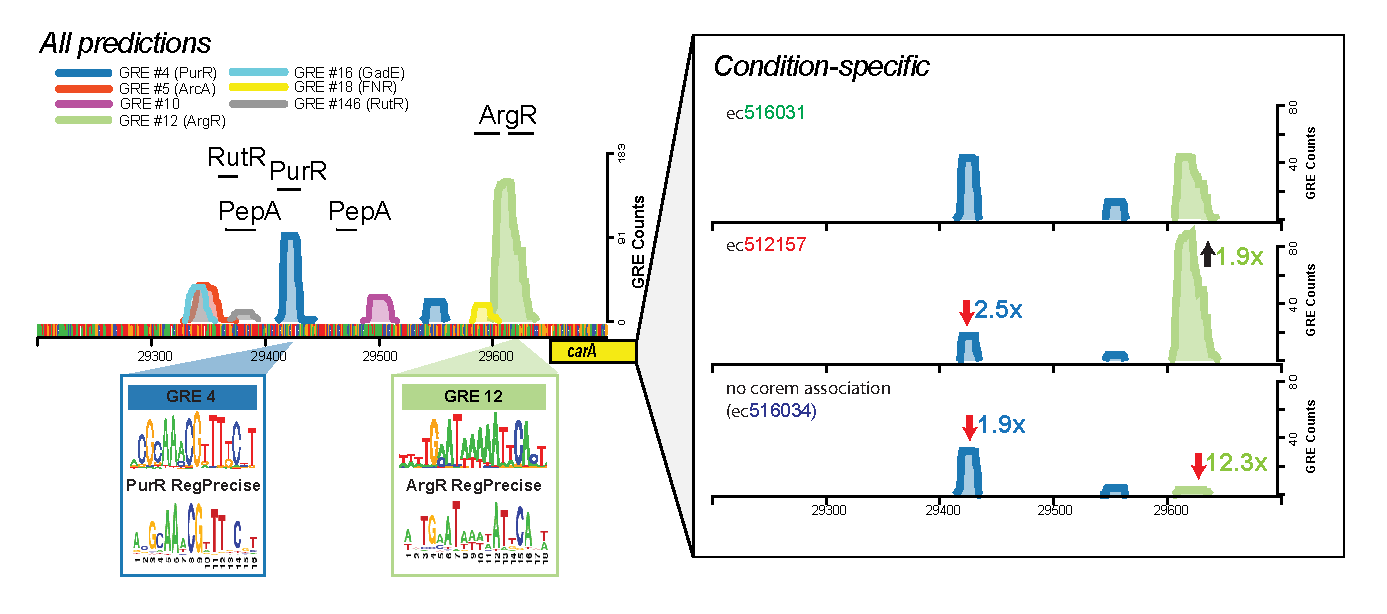
\includegraphics[width=\textwidth]{figures/egrin2_carA}
 	\caption[\egrine~Model Validation: Regulatory elements of \textit{carA}, \eco]{Predicted architecture of the \eco \textit{carA} promoter across all ensemble predictions (as in Figure \ref{fig:egrin2:2:C}). Horizontal bars above peaks mark experimentally characterized TF binding sites (RegulonDB). Significant GRE matches to characterized \eco binding sites in RegulonDB are indicated in parentheses. (Right) Condition-specific states of the \textit{carA} promoter. Variation in conditional discovery of GREs (counts and fold-change relative to ec516031, top) suggests when they are “active” across three different subsets of experimental conditions in the carA promoter. (Bottom). Condition subsets correspond to co-regulation of \textit{carA} with genes in the nucleotide and pyrimidine corems (ec516031, ec512157) or environments where \textit{carA} is not co-regulated with genes in any corem (ec516034). Motif logos for GRE \#4 (PurR) and GRE \#12 (ArgR) from the \egrine~predictions compared to logos from RegPrecise. 

}
    \label{fig:egrin2:2:D}
\end{figure}

\begin{figure}[h!]
    \centering
    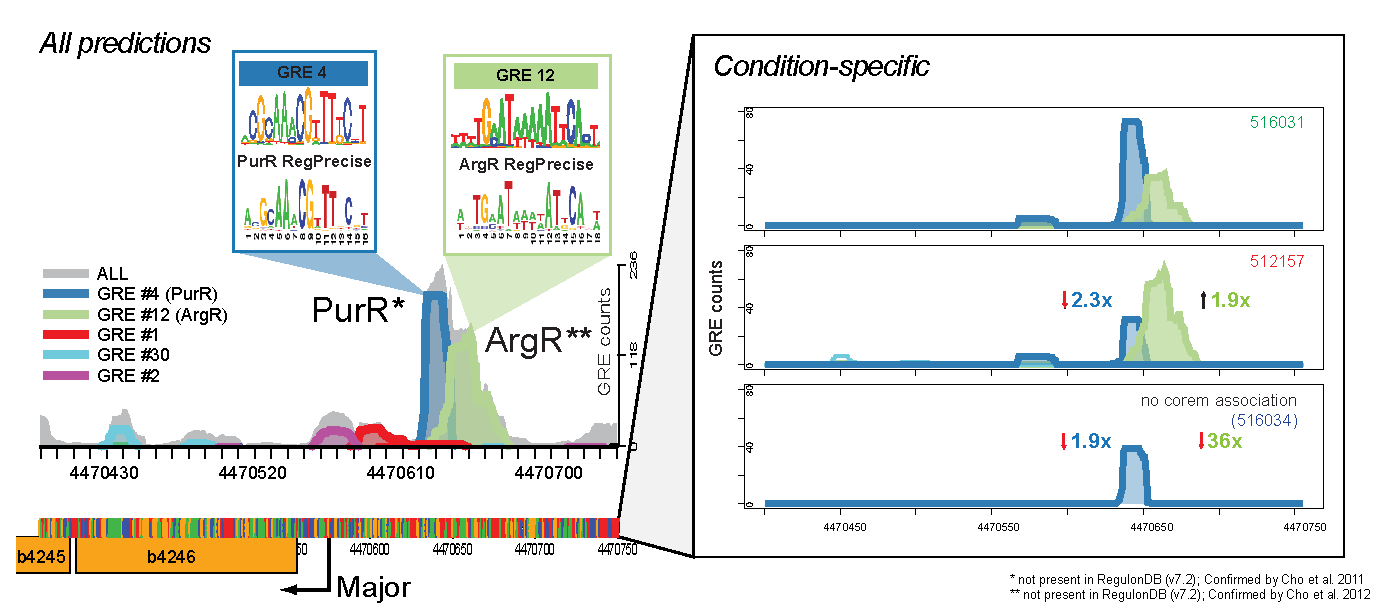
\includegraphics[width=\textwidth]{figures/pyrL}
 	\caption[\egrine~Model Validation: Regulatory elements of \textit{pyrL}, \eco]{Differential GRE activity in \textit{pyrL} promoter, \textit{E. coli}. (Left) Predicted promoter architecture for \textit{E. coli pyrL} (b4246). Overlapping GREs matching to PurR (GRE \#4) and ArgR (GRE \#12) were detected upstream of \textit{pyrL}. These sites were not annotated in RegulonDB, but were validated in independent ChIP-chip experiments \cite{cho_purr_2011,cho_deciphering_2012}. Transcription start site indicated with arrow. (Right) Condition-specific promoter architectures for \textit{E. coli pyrL} (as in Figure \ref{fig:egrin2:2:D}). Variation in predicted GRE activity across three different subsets of experimental conditions (counts and fold-change) for two GREs in the \textit{pyrL} promoter. Experimental subsets correspond to conditions under which at least one of three nucleotide biosynthetic corems is regulated (denoted by colored names at top-right of each plot)
}
    \label{fig:pyrL}
\end{figure}

We were most interested, however, to understand the consequences of conditional regulation at ArgR and PurR-associated GREs on variable expression of \textit{carA} in different environments. Indeed, \egrine~predicts three condition-specific states of the \textit{carA} promoter with respect to when PurR- and ArgR-matched GREs are conditionally active: (1) high PurR and high ArgR, (2) low PurR and high ArgR, and (3) high PurR and low ArgR (Figure \ref{fig:egrin2:2:D}). Interestingly, two of these promoter states correspond to co-regulation of \textit{carA} with a different combination of genes (i.e., different corems), functionally separating pyrimidine from purine biosynthesis (Figure \ref{fig:egrin2:4:B}), while the third state is not associated with co-regulation of \textit{carA} with the genes of any corem. Thus, the context in which GREs are active accurately explains when and how genes are co-regulated in different overlapping combinations to perform distinct functions.

\subsection{Conditionally active GREs within operons generate multiple, overlapping, and differentially regulated transcript isoforms}

Some of the GREs discovered in \egrine~occur in non-canonical locations and lead to unexpected transcriptional behaviors, such as the subdivision of operons into multiple transcriptional units.  Previously, we reported pervasive modulation of the \halo transcriptome structure by transcriptional elements that are located within operons and coding regions \cite{koide_prevalence_2009}. \egrine~recapitulated this phenomenon by sub-dividing operon genes into different corems. In all, the model predicted that nearly one-third of all \halo operons generate multiple transcript isoforms (Figure \ref{fig:nirH}, Figure \ref{fig:sdh},Figure \ref{fig:vng2211h}, Chapter \ref{chap:2} for details). Nearly half of these predictions of conditional operon structures were corroborated by experimentally mapped transcriptional breaks (hypergeometric pval = $4.2\times10^{-3}$; Table S7; Koide et al., 2009). Often, these transcript boundaries were adjacent to GREs that coincide with experimentally determined TFB-binding sites (\cite{facciotti_general_2007}; Figure \ref{fig:egrin2:3:A}), reinforcing the accuracy of \egrine~predictions.

\begin{figure}[h!]
    \centering
    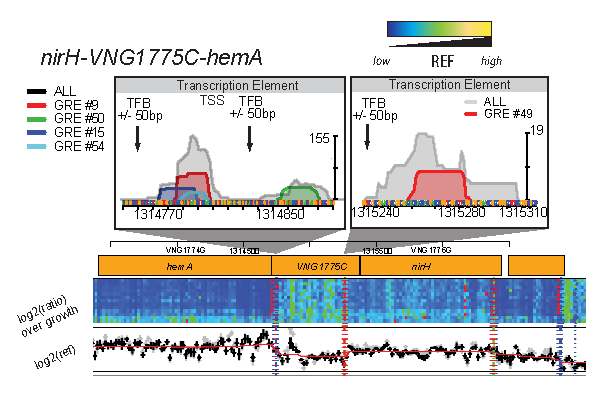
\includegraphics[width=0.75\textwidth]{figures/nirH}
 	\caption[Transcriptional evidence for multiple transcript isoforms from the same operon: \textit{nirH-VNG1775C-hemA}, \halo ]{GREs regulate multiple transcript isoforms from operons in \textit{H. salinarum, nirH-VNG1775C-hemA}. GREs located inside operons coincide with experimentally measured transcriptional break sites. Experimentally determined tran- scription break sites (red dashed lines) above expression profiles of these regions across growth (heatmap \cite{koide_prevalence_2009} and ChIP-chip TFBs \cite{facciotti_general_2007}, vertical arrows) support the role of GREs in regulating segmentation of the operon in certain conditions. Insets contain regions immediately surrounding transcriptional break sites, including counts of GREs discovered at these locations.
}
    \label{fig:nirH}
\end{figure}

\begin{figure}[h!]
    \centering
    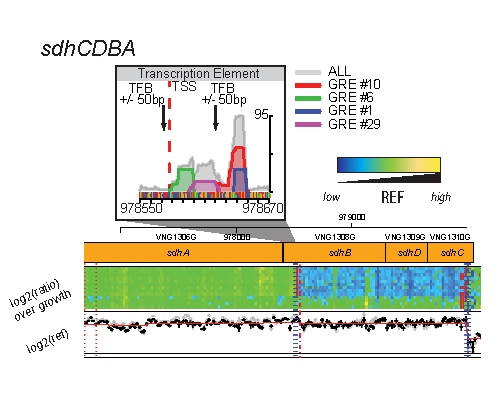
\includegraphics[width=0.75\textwidth]{figures/sdh}
 	\caption[Transcriptional evidence for multiple transcript isoforms from the same operon: \textit{sdhCDBA}, \halo ]{GREs regulate multiple transcript isoforms from operons in \textit{H. salinarum, sdhCDBA}. Caption details included in Figure \ref{fig:nirH}.}
    \label{fig:sdh}
\end{figure}

\begin{figure}[h!]
    \centering
    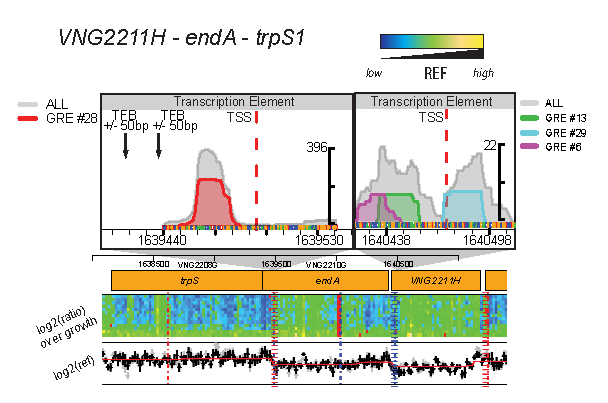
\includegraphics[width=0.75\textwidth]{figures/vng2211h}
 	\caption[Transcriptional evidence for multiple transcript isoforms from the same operon: \textit{VNG2211H-endA-trpS1}, \halo ]{GREs regulate multiple transcript isoforms from operons in \textit{H. salinarum, VNG2211H-endA-trpS1}. Caption details included in Figure \ref{fig:nirH}.}
    \label{fig:vng2211h}
\end{figure}

\begin{figure}[h!]
    \centering
    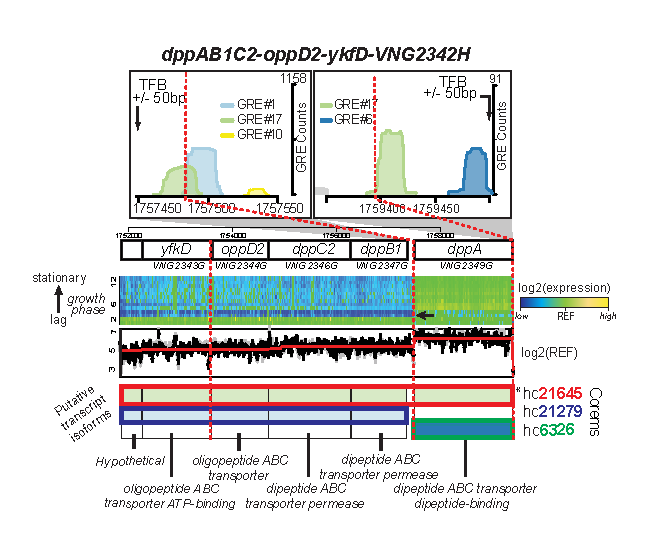
\includegraphics[width=0.8\textwidth]{figures/egrin2_dpp_1}
 	\caption[Transcriptional evidence for multiple transcript isoforms from the same operon, \halo ]{(Top) Predicted GREs located within (left) and upstream of (right) the \halo \textit{dpp} operon. Locations of experimentally mapped TFB binding sites (vertical arrows; \cite{facciotti_general_2007}), and experimentally mapped transcription break sites (vertical red dashed lines, see (B); \cite{koide_prevalence_2009}) are indicated. Locations of predicted GREs relative to coding segments of the \textit{dpp} operon. (Midlle) Expression changes during growth in the genomic region covering the \textit{dpp} operon measured by high-resolution tiling microarray. Raw RNA hybridization signal from mid-log growth phase indicated below. (Bottom) Three predicted transcripts from the \textit{dpp} operon. Internal colors correspond to the GREs putatively responsible for regulating each transcript (shown at top, derived from corem membership in Figure \ref{fig:egrin2:3:B}). Boxed colors indicate corem membership for each transcript (described in Figure \ref{fig:egrin2:3:B}). Red dashed lines indicate experimentally measured transcription break sites. Transcriptional break at lag phase highlighted by an arrow. Functional annotation for each gene located at bottom.
}
    \label{fig:egrin2:3:A}
\end{figure}

We further investigated whether \egrine~provides insight into downstream consequences of differentially regulating multiple transcript isoforms from the same operon. The \textit{dppAB1C2-oppD2-ykfD-VNG2342H} operon (hereafter the ‘\textit{dpp} operon’) in \halo encodes an ATP-dependent dipeptide transporter. Some periplasmic binding proteins (like \textit{dppA}) have the reported ability to function in conjunction with different ABC transport systems, giving support to the hypothesis that \textit{dppA} can be regulated independently \cite{higgins_binding_1990}. Despite high co-expression of the entire operon in the training data (mean R$^{2}$ = 0.6 across 1495 conditions), \egrine~predicted that the genes of this operon are transcribed as three different isoforms, each co-regulated with genes of a different corem: (1) the entire operon (hc21645 –“\textit{dpp} corem”), (2) the entire operon except the leader gene, \textit{dppA} (hc21279 –“permease corem”), and (3) just \textit{dppA} (hc6326 –“leader corem”). These predicted isoforms were verified by experimentally mapped transcript boundaries (Figure \ref{fig:egrin2:3:B}). Each of these corems contains a different dpp isoform and is enriched for a different biological function, including vitamin biosynthesis, porphyrin metabolism, and purine biosynthesis, respectively (Figure \ref{fig:egrin2:3:B}). Predicted differential regulation of the core permease (\textit{dppB1C2-oppD2-ykfD-VNG2342H}) with porphyrin metabolism genes in the permease corem is consistent with the reported capability of this transporter system to uptake heme when it functions with a different solute binding protein (i.e., without \textit{dppA}; \cite{letoffe_housekeeping_2006}). Overall, \egrine~provided insight into the distinct environment-dependent functional associations of each transcript isoform.   

Further, \egrine~revealed that segmentation of the \textit{dpp} operon into multiple corems is mediated by conditionally active GREs located both upstream and internal to the operon. For example, \egrine~predicted that GRE \#6 was responsible for disassociating \textit{dppA} transcription from the remainder of the operon. Interestingly, GRE \#6 was also discovered in the promoters of nearly all of the other genes in the leader corem (Figure \ref{fig:egrin2:3:A}, Figure \ref{fig:dpp_networks}, Table S8). Similarly, GRE \#1 was implicated in co-regulating the permease-encoding transcript with other genes in the permease corem, and GRE \#17 for co-regulating the entire operon with other genes in the \textit{dpp} corem. \egrine~ also predicted specific segmentation pattern of the dpp-operon during ‘lag growth phase’. This prediction was verified upon observing that a transcript break appears downstream to \textit{dppB1} precisely when a batch culture transitions from lag to log phase of growth (indicated by arrow in Figure \ref{fig:egrin2:3:A} heatmap). This is just one of 98 operons with experimentally validated conditional isoforms in \halo. For each instance, a similar correspondence between mechanism, context, and function could be demonstrated (Figure \ref{fig:nirH}, Figure \ref{fig:sdh},Figure \ref{fig:vng2211h}, and online).   Interestingly, even in \eco, where previous studies report a single transcript for the \textit{dpp} operon \cite{abouhamad_dipeptide_1994}, \egrine~ discovered that it is actually transcribed as multiple, condition-specific transcript isoforms, each of which participates in a different physiological process (Figure E5A).

\begin{figure}[h!]
    \centering
    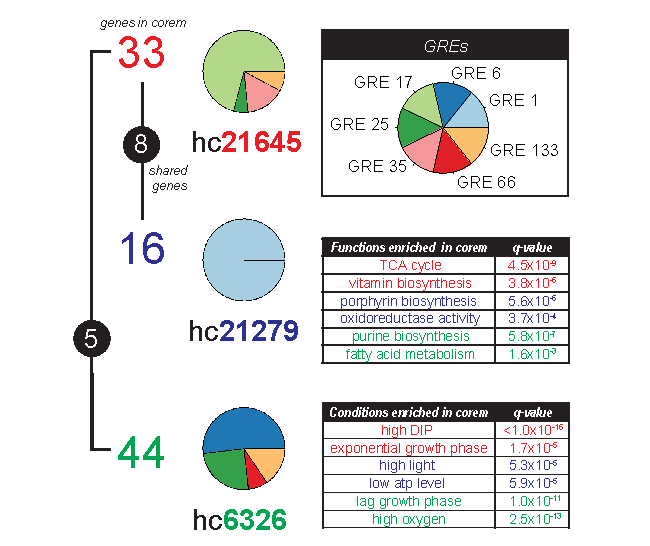
\includegraphics[width=0.65\textwidth]{figures/egrin2_dpp_2}
 	\caption[Functional consequences of multiple transcript isoforms from the same operon, \halo]{ (Left) Three \halo corems model differential regulation of \textit{dpp} operon isoforms: (1) the entire operon (hc21645 –“\textit{dpp} corem”; top); (2) five tail genes, excluding \textit{dppA} (hc21279 –“permease corem”; center); and (3) the leader gene, \textit{dppA} (hc6326 –“leader corem”; bottom). Colored numbers denote quantity of genes in each corem; numbers in black shaded circles indicate the number of genes shared between corems. Pie charts represent average predicted influence of GREs on regulation of genes in each corem (see Figure E3B for detail). (Top-Right) Pie chart key indicates GRE identity. (Bottom-Right) Tables list enriched gene functions \cite{dennis_david:_2003} and environmental conditions for each of the corems (computed using the environmental ontology; see Chapter \ref{chap:2})
}
    \label{fig:egrin2:3:B}
\end{figure}

\begin{figure}[h!]
    \centering
    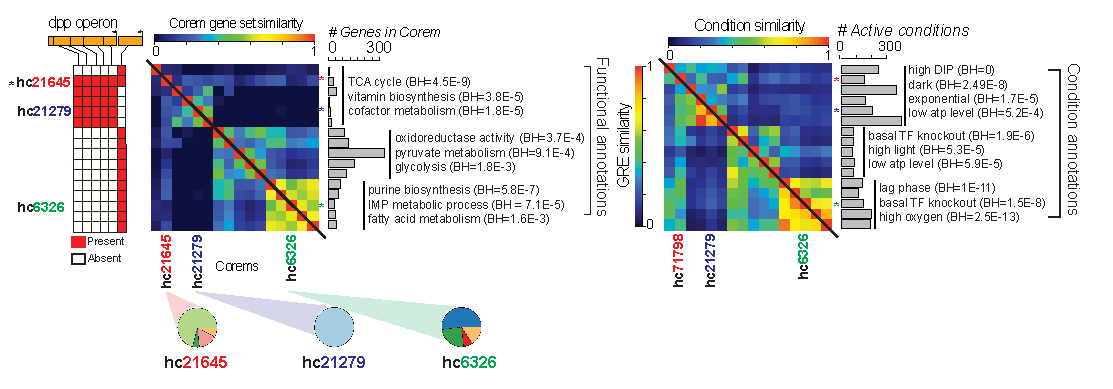
\includegraphics[width=\textwidth]{figures/dpp_heatmaps}
 	\caption[Alternate regulatory modes for \textit{dpp} operon predicted by corems, \halo]{Corems group together functionally related sets of genes that are co-regulated in similar environments by similar factors (Left) Presence/absence of \textit{dpp} operon genes in corems. Three classes of corems exist for the dpp operon: (1) the entire operon (e.g.hc21645), (2) the leader gene dppA (e.g.hc6326), and (3) five ``tail'' genes excluding \textit{dppA} (hc21279). (Middle) Gene similarity between corems (heatmap, Jaccard index). Functional annotations of genes in three highly similar clusters of corems to right. GRE composition for three corems shown below (pie chart, see Figure \ref{fig:corem_gres}). (Right). Similarity of conditions regulated (heatmap, upper triangle, Jaccard index) and GREs (heatmap, lower triangle, Jaccard index) among corems. Ordering is identical to (Middle). Environmental Ontology term enrichment (see Chapter \ref{chap:2}) for three clusters depicted to right.
}
    \label{fig:dpp_heatmaps}
\end{figure}

\begin{figure}[h!]
    \centering
    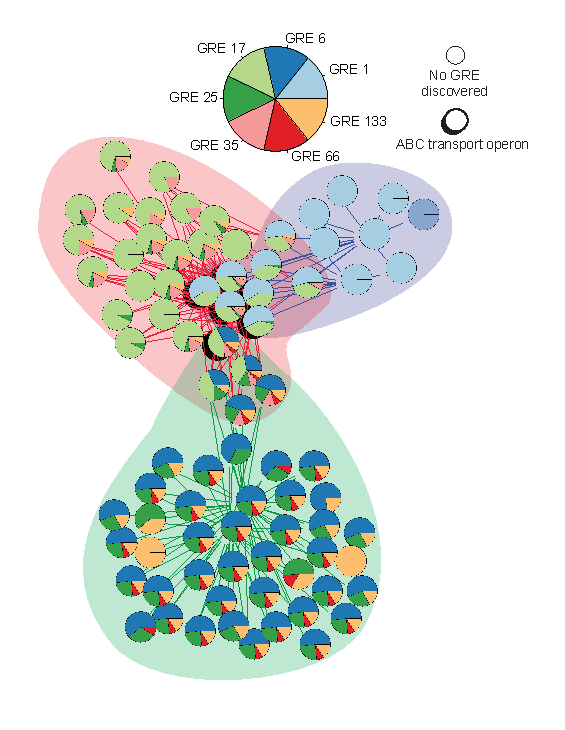
\includegraphics[width=0.75\textwidth]{figures/dpp_networks}
 	\caption[Network representation of transcriptional isoforms for the \textit{dpp} operon predicted by corems, \halo]{Network representation of transcriptional isoforms for the \textit{dpp} operon predicted by corems. Genes represented by circles. Edge colors and colored region behind the network indicate corem membership. Pie charts reflect GRE composition of each gene (see Figure \ref{fig:corem_gres}). Key for pie charts at top. Shading behind nodes (center of network) indicates dpp operon genes.
}
    \label{fig:dpp_networks}
\end{figure}

\begin{figure}[h!]
    \centering
    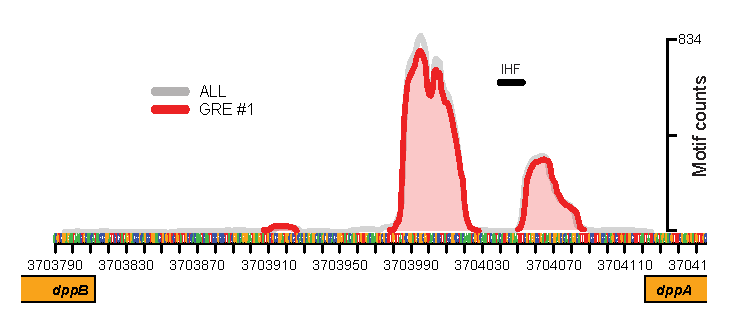
\includegraphics[width=0.75\textwidth]{figures/dpp_ecoli}
 	\caption[Evidence for condition-specific transcript isoforms of the \textit{dpp} operon in \textit{E. coli}]{EGRIN 2.0 predicts conditional modulation of \textit{dpp} operon in \textit{E. coli} as well. Promoter architecture within intergenic space between \textit{dppA} and \textit{dppB} suggested locations for TF binding internal to the operon (as in Figure \ref{fig:egrin2:3:A}). GRE binding sites are proximal to an experimentally characterized IHF binding site (black horizontal bar; RegulonDB).
}
    \label{fig:dpp_ecoli}
\end{figure}

While we were aware of extensive transcriptional heterogeneity within operons in \halo, we were surprised that \egrine~ predicted that the same phenomenon also occurred extensively in \eco. To see if this were true, we mapped the \eco global transcriptome structure across varying phases of growth in rich media using a densely tiled microarray (see Chapter \ref{chap:2}). We used this new gene expression data set to identify the corems in which different combinations of operon genes (i.e., transcript isoforms) were co-regulated in some or all phases of growth, and to characterize transcriptional breaks using previously developed methodologies \cite{koide_prevalence_2009}. We observed transcriptional breaks in nearly 20 percent of operons (including the \eco \textit{dpp} operon) just over this 9-time point growth study, validating \egrine~ prediction that nearly one-quarter of all \eco operons have conditional isoforms during varying stages of growth (hypergeometric pval = $1.07\times10^{-5}$, Figure \ref{fig:dpp_ecoli_expression}, Figure \ref{fig:galE}, Figure \ref{fig:ptsh}, Table S7). Experimental validation of this enormous transcriptional heterogeneity among operons in \eco demonstrates the power of \egrine~ to distinguish nuanced patterns in complex data, and provide both mechanistic explanation and context for when and why the novel phenomena might occur.

\subsection{Some TFs act similarly across certain environments to co-regulate functionally-related subsets of genes across their respective regulons}

We investigated whether \egrine~ provides insights into context-dependent  differential regulation of branched metabolic pathways – even those that have been meticulously studied for decades, such as \textit{de novo} biosynthesis of nucleotides in \eco \cite{neidhardt_escherichia_1996}. At least seven GREs were implicated in partitioning (purine biosynthesis: ec516034 –“purine corem”; pyrimidine biosynthesis: ec512157 –“pyrimidine corem”) or co-regulating (ec516031 –“nucleotide corem”) nucleotide biosynthesis into multiple overlapping corems (Figure \ref{fig:egrin2:4:A}, Figure \ref{fig:purR_heatmap}, Figure \ref{fig:purR_network}). The genome-wide locations for four of these GREs significantly overlapped with known binding locations for PurR, ArgR, MetJ, and IclR. Partitioning and co-regulation of purine and pyrimidine biosynthesis can be attributed to the location of these GREs in promoters of pathway genes, including \textit{carA}, and the environments in which they are predicted to be active (Figure \ref{fig:egrin2:2:D}). \egrine~ predicts, for example, that MetJ (GREs \#19, \#87) acts in conjunction with PurR (GRE \#4) to differentially regulate genes specific to the pyrimidine biosynthetic branch (pyrimidine corem), while (yet to be identified) TFs that bind GREs \#2 and \#206 function with PurR (GRE \#4) to regulate genes in the purine branch (purine corem) (Figure \ref{fig:egrin2:4:B}). The organization of these GREs within and across promoters, and the environments in which they act to mediate regulation by specific TFs, generates complex co-expression patterns among different combinations of genes in the three corems of this highly canalized pathway (filled violin plots, Figure \ref{fig:egrin2:4:C}). These conditional co-expression patterns predict that in certain environments the two branches are differentially regulated, while in others they are co-regulated as one unit. Consistent with this observation, fitness consequences of deleting genes in these corems vary across conditions (Figure \ref{fig:egrin2:4:D}, Figure \ref{fig:purR_corem_fitness}, Figure \ref{fig:purR_corem_fitness_specific}). For instance, knockouts of genes in all three corems have similar consequences on fitness in the presence of glucose. By contrast, in the presence of the toxic ionophore carbonyl cyanide m-chlorophenyl hydrazone (CCCP), only knockouts of genes in the nucleotide corem significantly alter fitness.

\begin{figure}[h!]
    \centering
    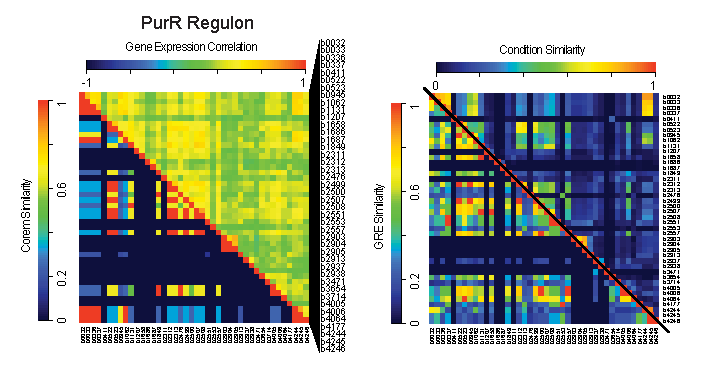
\includegraphics[width=\textwidth]{figures/purR_heatmap}
 	\caption[Corems model the mechanistic basis for conditional subdivision of the PurR regulon, \textit{E. coli.}]{(Left) Corems identify the most highly correlated subgroupings of genes in PurR regulon. Gene expression correlation across all experiments (upper triangle) compared to similarity of corem membership (lower-triangle, Jaccard index) for genes of the PurR regulon (gene identifiers expanded to right). (Right) Similarity of regulated conditions (upper triangle, Jaccard index) and GREs com- position for these genes (bottom triangle, Jaccard index). Consistent patterns of conditional-activity and GRE composition in their promoter regions further supports subdivision of PurR genes into separate corems. Gene order is same as left.
}
    \label{fig:purR_heatmap}
\end{figure}

\begin{figure}[h!]
    \centering
    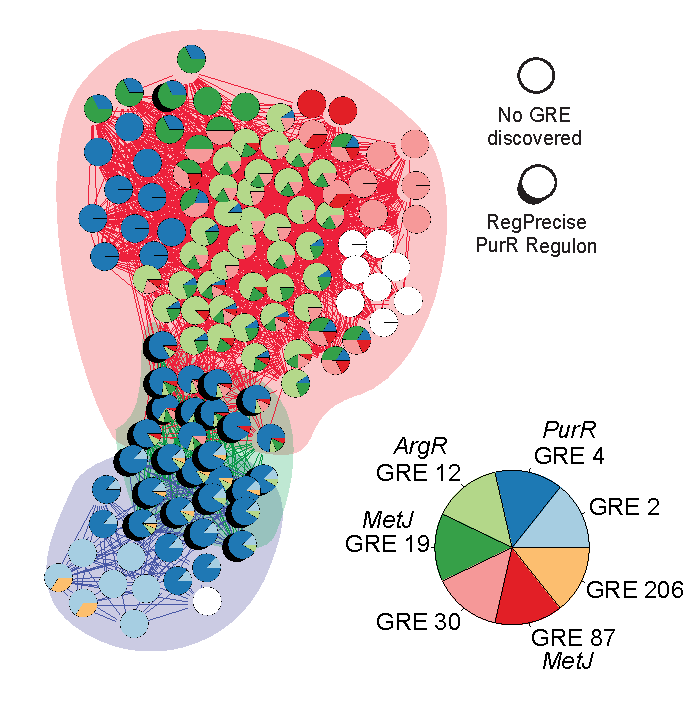
\includegraphics[width=0.75\textwidth]{figures/purR_network}
 	\caption[Corems integrate diverse regulatory mechanisms, \textit{E. coli}]{Network representation for three corems described in Figure \ref{fig:egrin2:4:A}. Genes are represented by circles. Edge colors and colored region behind the network indicate corem membership. Pie charts reflect GRE composition of each gene (see Figure \ref{fig:corem_gres}). Key for pie charts at bottom. GRE-TF matches are indicated. Shading behind nodes denotes PurR regulon genes. At least 7 different mechanisms regulate the expression of these genes.
}
    \label{fig:purR_network}
\end{figure}

\begin{figure}[h!]
    \centering
    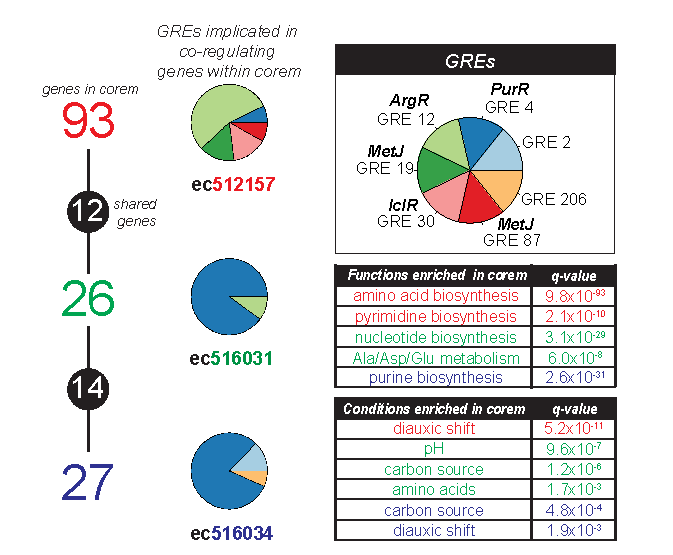
\includegraphics[width=0.65\textwidth]{figures/egrin2_ecoli_1}
 	\caption[Condition-specific subdivision and coordination of the nucleotide biosynthesis pathway, \eco: functional segregation across corems]{Genes of nucleotide biosynthesis are distributed in overlapping combinations across three \eco corems: purine (ec516034 –“purine corem”), pyrimidine (ec512157–“pyrimidine corem”), or both pathways (ec516031 –“nucleotide corem”). (Left) Gene membership and overlap for the three corems as in Figure \ref{fig:egrin2:3:B}. Pie charts indicate average GRE composition across all gene promoters in each corem (see Figure \ref{fig:corem_gres} for detail). (Top-Right Inset) GRE key for pie charts. Matches to TFs in RegulonDB noted above the GRE name. (Bottom-Right) Tables list enriched gene functions \cite{dennis_david:_2003} and environmental conditions for each of the corems (see Chapter \ref{chap:2}). 
}
    \label{fig:egrin2:4:A}
\end{figure}

\begin{figure}[h!]
    \centering
    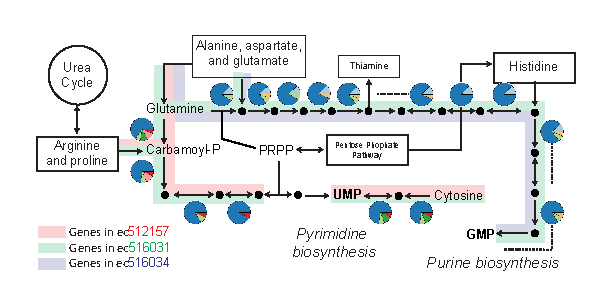
\includegraphics[width=0.8\textwidth]{figures/egrin2_ecoli_2}
 	\caption[Corems segment the nucleotide biosynthesis pathway, \eco]{A portion of the nucleotide biosynthetic pathways, near the branch point dividing purine (top) and pyrimidine (bottom) biosynthesis. Pie charts represent GRE composition in each gene promoter (Key in Figure \ref{fig:egrin2:4:A}). Operons denoted by dashed lines, with only the leader gene’s promoter architecture shown.
}
    \label{fig:egrin2:4:B}
\end{figure}

\begin{figure}[h!]
    \centering
    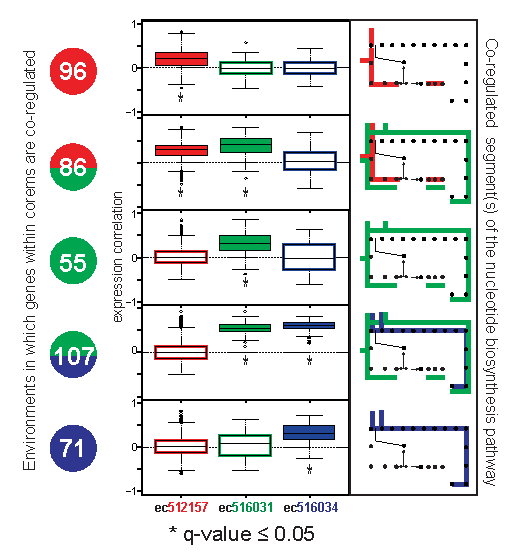
\includegraphics[width=0.6\textwidth]{figures/egrin2_ecoli_3}
 	\caption[Differential co-expression across the nucleotide biosynthesis pathway, \eco ]{Condition-specific co-expression of genes across the three corems. (Right) The active segments of nucleotide biosynthesis (as in Figure \ref{fig:egrin2:4:B}) are color-matched to corems. (Center) Box plots plots show distributions of expression correlations between genes within each corem in relevant environmental conditions, when they are predicted to be co-regulated. Color fill and asterisks indicate corems with significantly low relative standard deviation (RSD; |σ/μ|; FDR ≤ 0.05). (Left) Colored circles indicate when genes within which corem(s) are predicted to be co-regulated (color) under how many conditions (number). 
}
    \label{fig:egrin2:4:C}
\end{figure}

\begin{figure}[h!]
    \centering
    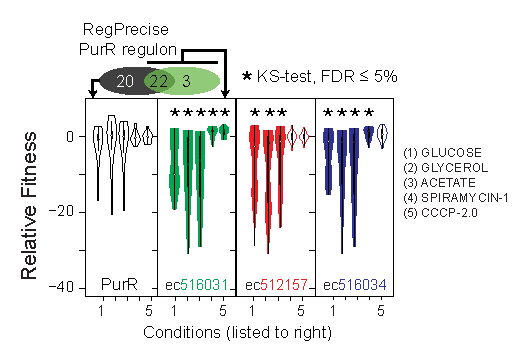
\includegraphics[width=0.8\textwidth]{figures/egrin2_ecoli_4}
 	\caption[Condition-specific fitness contributions across nucleotide biosynthesis pathway predicted by corems, \eco]{Distributions of relative fitness values for gene deletions in the three corems, as well as 20 of the 42 PurR regulon genes not modeled by ec516031 (black) across 5 representative conditions (condition identifiers listed to right, additional conditions in Figure \ref{fig:purR_corem_fitness_specific}). Asterisks denote conditions in which the distribution of fitness values is statistically significant (relative to the distribution of fitness values for all genes in that condition).
}
    \label{fig:egrin2:4:D}
\end{figure}

\begin{figure}[h!]
    \centering
    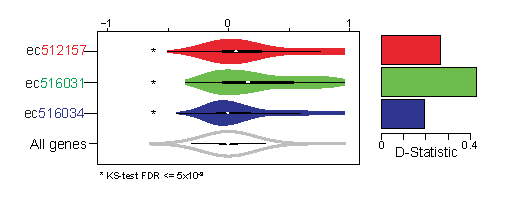
\includegraphics[width=0.8\textwidth]{figures/purR_corem_fitness}
 	\caption[Genes from corems related to nucleotide biosynthesis have highly similar fitness effects when they are deleted]{(Left) Violin plot shows distribution of all fitness correlations for genes in three nucleotide biosynthesis-associated corems compared to all genes in the data set. (Right) KS D-Statistic relates to enrichment for highly correlated gene-gene fitness associations in the corems. All three corems enrich for similar fitness effects (KS FDR $<$ 5 × $10^{−9}$)
}
    \label{fig:purR_corem_fitness}
\end{figure}

\begin{figure}[h!]
    \centering
    \includegraphics[width=0.8\textwidth]{figures/purR_corem_fitness_specific}
 	\caption[Corems model fitness effects that occur in specific environments]{Violin plots show distribution of relative fitness among corems across conditions (negative values indicate lower fitness relative to WT). Brief condition descriptions are displayed below. Shading within the violin plot indicates that the distribution of fitness values is significantly in that condition (KS-test FDR $\leq$ 0.05). Fitness values for the subset of genes from the PurR regulon that do not occur in ec516031 are displayed to the left. These genes do not have significant fitness effects in any of the environments tested.
}
    \label{fig:purR_corem_fitness_specific}
\end{figure}

This example highlights two important features of \egrine~ and corems. First, \egrine~ can distinguish co-regulation by independent, similarly-acting TFs, even though their targets are co-expressed. Further, corems group together genes that are functionally-related even though their co-regulation is mediated by different mechanisms, demonstrating how conditional TF-influences in a GRN coordinate transcription of genes from different regulons whose deletions have highly correlated fitness consequences (Table \ref{tab:table1}). Genes of the pyrimidine corem, for example, are co-regulated by as many as five TFs. Even though promoters of each of the genes in this corem contain distinct compositions of GREs (Figure \ref{fig:purR_network}, Tables S9-S10), their expression is highly coordinated across a broad range of conditions. Interestingly and counter to our expectation, transcript level changes of the similarly acting TFs are not highly correlated. Instead, we discovered correlated changes in the concentrations of effector molecules, which allosterically regulate the activities of these TFs, suggesting that coordinate regulation of genes in the pyrimidine corem is a direct consequence of metabolic dynamics (Figure \ref{fig:purR_effector}; \cite{ishii_multiple_2007}).

\begin{figure}[h!]
    \centering
    \includegraphics[width=0.8\textwidth]{figures/purR_effector}
 	\caption[Metabolite correlations may explain co-regulation within metabolically-linked corems]{(Left) Expression correlation for TFs associated with three corems described in the text (ec516031,ec512157,ec516034). (Right) Correlation allosteric regulators for these TFs. TF regulated by each biomolecule listed in parentheses. Red boxes indicate PurR-ArgR and their corresponding effector molecules. Data from \cite{ishii_multiple_2007}.
}
    \label{fig:purR_effector}
\end{figure}

% Table 1
% Table generated by Excel2LaTeX from sheet 'highfit_regprecise_sub.txt'
\begin{table}[htbp]
  \centering
  \caption{Corems group together genes from different regulons with highly correlated fitness effects}
  \resizebox{\columnwidth}{!}{%
    \begin{tabular}{c c p{5cm} c c c}
    \toprule
    \multicolumn{1}{c}{\textbf{Gene 1}} & \multicolumn{1}{c}{\textbf{Gene 2}} & \multicolumn{1}{c}{\textbf{Fitness correlation}} & \multicolumn{1}{c}{\textbf{Regulon Gene 1}} & \multicolumn{1}{c}{\textbf{Regulon Gene 2}} & \multicolumn{1}{c}{\textbf{Corems}} \\
    \midrule
    \multicolumn{1}{c}{\textit{b3774}} & \multicolumn{1}{c}{\textit{b3959}} & \multicolumn{1}{c}{0.959012} & \multicolumn{1}{c}{IlvY} & \multicolumn{1}{c}{ArgR} & \multicolumn{1}{c}{512157} \\
    \multicolumn{1}{c}{\textit{b2913}} & \multicolumn{1}{c}{\textit{b3829}} & \multicolumn{1}{c}{0.938764} & \multicolumn{1}{c}{PurR} & \multicolumn{1}{c}{MetR} & \multicolumn{1}{c}{512157} \\
    \multicolumn{1}{c}{\textit{b3829}} & \multicolumn{1}{c}{\textit{b3959}} & \multicolumn{1}{c}{0.934393} & \multicolumn{1}{c}{MetR} & \multicolumn{1}{c}{ArgR} & \multicolumn{1}{c}{512157;554056} \\
    \multicolumn{1}{c}{\textit{b2913}} & \multicolumn{1}{c}{\textit{b3941}} & \multicolumn{1}{c}{0.932025} & \multicolumn{1}{c}{PurR} & \multicolumn{1}{c}{MetR} & \multicolumn{1}{c}{512157} \\
    \multicolumn{1}{c}{\textit{b3957}} & \multicolumn{1}{c}{\textit{b3941}} & \multicolumn{1}{c}{0.931565} & \multicolumn{1}{c}{ArgR} & \multicolumn{1}{c}{MetR} & \multicolumn{1}{c}{512157;554056} \\
    \multicolumn{1}{c}{\textit{b3172}} & \multicolumn{1}{c}{\textit{b3829}} & \multicolumn{1}{c}{0.930382} & \multicolumn{1}{c}{ArgR} & \multicolumn{1}{c}{MetR} & \multicolumn{1}{c}{512157;554056} \\
    \multicolumn{1}{c}{\textit{b2913}} & \multicolumn{1}{c}{\textit{b3774}} & \multicolumn{1}{c}{0.927776} & \multicolumn{1}{c}{PurR} & \multicolumn{1}{c}{IlvY} & \multicolumn{1}{c}{512157;512477} \\
    \multicolumn{1}{c}{\textit{b3941}} & \multicolumn{1}{c}{\textit{b3774}} & \multicolumn{1}{c}{0.927251} & \multicolumn{1}{c}{MetR} & \multicolumn{1}{c}{IlvY} & \multicolumn{1}{c}{512157} \\
    \multicolumn{1}{c}{\textit{b3960}} & \multicolumn{1}{c}{\textit{b3941}} & \multicolumn{1}{c}{0.921375} & \multicolumn{1}{c}{ArgR} & \multicolumn{1}{c}{MetR} & \multicolumn{1}{c}{512157;554056} \\
    \multicolumn{1}{c}{\textit{b3941}} & \multicolumn{1}{c}{\textit{b3959}} & \multicolumn{1}{c}{0.921282} & \multicolumn{1}{c}{MetR} & \multicolumn{1}{c}{ArgR} & \multicolumn{1}{c}{512157;554056} \\
    \bottomrule
    \end{tabular}%
    }
  \label{tab:table1}%
\end{table}%


Second, \egrine~ predicts that not all locations that match to the same GRE are functionally equivalent in all environments. Accordingly, using corems we can discern and explain why genes regulated by the same TF exhibit different expression patterns in certain environments. For example, out of the 42 PurR-regulated genes (assigned by RegPrecise), expression changes of the 14 that are grouped into the purine corem are better correlated with each other and genes of this corem than they are to the portion of the PurR regulon that was left out (t-test, pval $< 2.2\times10^{-16}$, Figure \ref{fig:egrin2:5:A}). Consistent with this observation, PurR is predicted to play a variable role in regulation of genes across the three corems (from being highly important for the nucleotide corem, to being marginally important for the pyrimidine corem, Figure \ref{fig:egrin2:4:A}). We hypothesized that the degree to which PurR is implicated in regulating genes within each corem is a good predictor of target-specific expression consequences of knocking out this TF. To test this hypothesis we analyzed global transcriptional changes in both wild type (WT) and $\Delta$purR deletion strains of \eco grown in the presence of adenine \cite{cho_purr_2011}. These data were obtained from experiments that were not included in construction of the \egrine~ model. Specifically, we calculated the relative standard deviation (a measure of co-regulation) for every PurR-associated corem in each of the two strains. As expected, genes in all three corems described above were co-regulated in the WT strain (FDR $<$ 0.05, Figure \ref{fig:egrin2:5:B}). Strikingly consistent with \egrine~predictions, the degree of dysregulation of genes within each of the three corems in the $\Delta$purR strain was proportional to the predicted magnitude of PurR influence. Maximal dysregulation of genes in the nucleotide corem and the purine corem, for example, was consistent with the predicted role of PurR as the primary regulator of genes in these corems (Figure fig:egrin2:5:C). Notably, the degree of disruption observed in these two corems surpasses that of the entire PurR regulon, suggesting that in the presence of adenine, PurR regulates only a subset of its target genes. These results illustrate how the concept of a corem captures the context in which TF binding to a GRE is functional, not just that the potential for TF-GRE interaction exists, which is how a regulon is defined.

\begin{figure}[h!]
    \centering
    \includegraphics[width=0.8\textwidth]{figures/egrin2_ecoli_expression_cor}
 	\caption[Transcriptional evidence for subdivision of regulons by corems]{Distributions of pairwise expression correlations among all genes in the PurR regulon (RegPrecise) compared to a subset of the regulon within corem ec516034, across all environmental conditions. Also shown are the total number of genes in each group, and the number of shared genes. The two distributions are significantly different (Welch Two Sample t-test, p $< 2.2^{-16}$).
}
    \label{fig:egrin2:5:A}
\end{figure}

\begin{figure}[h!]
    \centering
    \includegraphics[width=0.8\textwidth]{figures/egrin2_ecoli_ko_expression}
 	\caption[Corems with predicted influence from PurR (GRE \#4) are disrupted in $\Delta$purR mutant]{RSD of transcript level changes (resampled -log10(pval)) for the three corems in Figure \ref{fig:egrin2:4:A} in WT and $\Delta$purR strains of \eco (both grown with adenine). The dashed line delineates significant co-expression (p = 0.05). 
}
    \label{fig:egrin2:5:B}
\end{figure}

\begin{figure}[h!]
    \centering
    \includegraphics[width=0.8\textwidth]{figures/egrin2_ecoli_purR_predictive}
 	\caption[GRE \#4 influence predicts which corems are disrupted in $\Delta$purR mutant]{Relative RSD ($\Delta$purR/WT) for all seven GRE \#4-associated corems plotted as a function of the frequency with which GRE \#4 (PurR) is discovered within these corems. Composition of GREs discovered within each corem are shown as pie charts (as in Figure \ref{fig:egrin2:4:A}), with key in inset, top-right. Relative RSD of the RegPrecise PurR regulon is shown for reference (dotted horizontal line).
}
    \label{fig:egrin2:5:C}
\end{figure}

\section{Discussion}

\egrine~explains how microbes tailor transcriptional responses to varied environments by linking the genome-wide distribution of GREs to their organization and conditional activities within each promoter. The integrative model reveals the mechanisms by which microbes reuse genes in varying combinations to operationally link disparate processes and regulate flux through metabolic pathways. We have provided extensive validations for predictions made by \egrine~for a bacterium and an archaeon (Table 2). In addition, we also performed new experiments to validate a model prediction that widespread transcriptional activity at non-canonical locations within genes and operons was partly responsible for complex modulation of the \eco transcriptome during growth in rich media.  

Corems represent a fundamental organizing principle of GRNs that captures fitness-relevant associations among genes, forging a link between the environment-dependent dynamics of transcriptional control and phenotype. The conditional associations among genes across corems reflect the underlying structure of coupled changes in environmental factors, such as correlated changes in effector molecules. Comparative analyses of \egrine~models, therefore, could reveal the corems associated with unique and shared environmental structures that distinguish ecotypes of the same species.

\egrine~will provide context-relevant engineering strategies for synthetic biology because it models environment-dependent coordination of diverse regulatory mechanisms operating across the entire genome, including non-canonical locations. By teasing apart regulatory mechanisms that have indistinguishable outputs in certain environments, \egrine~offers multiple strategies for introducing new genes into the GRN. For instance, there are at least five distinct mechanisms responsible for co-regulating nearly 100 genes in the pyrimidine corem in \eco. This corem coordinates genes from various segments of amino acid biosynthesis pathways, including arginine biosynthesis, as well as the pentose phosphate pathway to synchronize inputs into nucleotide biosynthesis. The conditional grouping of genes into the pyrimidine corem explains the previous observation that genes of arginine biosynthesis are repressed upon adenine addition \cite{cho_purr_2011}. \egrine~predicts that this coordination of nucleotide and arginine biosynthesis is accomplished by an equivalency of PurR and ArgR activities under these conditions (possibly due to correlated changes in effector molecules), rather than by direct regulation of arginine biosynthesis genes by PurR. Not surprisingly, subsets of genes within this corem belong to alternate regulatory programs (corems) under different environmental contexts. Thus, depending on the objective, we can select a reengineering strategy from a library of mechanisms that already exist within the GRN of an organism. Future work to translate the \egrine~model into the language of synthetic biology will enable systems-level reengineering of an organism.

    % ========== Chapter 4
 
\chapter {\uppercase{Evolution of gene regulatory networks in prokaryotes}}
\label{chap:4}

The evolutionary success of an organism is a testament to its inherent capacity to keep pace with environmental conditions that change over short and long periods. Mechanisms underlying adaptive processes are being investigated with renewed interest and excitement. This revival is partly fueled by powerful technologies that can probe molecular phenomena at a systems scale. Such studies provide spectacular insight into the mechanisms of adaptation, including rewiring of regulatory networks via natural selection of horizontal gene transfers, gene duplication, deletion, readjustment of kinetic parameters, and myriad other genetic reorganizational events. In this chapter, I discuss advances in our understanding of principles that shape evolution of gene regulatory networks (GRNs) for dynamic adaptation to environmental change. \\

\noindent This chapter has been adapted from: \\

\noindent Brooks AN, Turkarslan S, Beer KD, Lo FY, Baliga NS. Adaptation of cells to new environments. (2011) \emph{Wiley Interdiscip Rev Syst Biol Med}. 3(5): 544–561\\

\paragraph{Chapter Highlights}

\begin{itemize}
\item Microbes have adapted to diverse environmental conditions 
\item Mechanism of adaptation depends on how fast and frequently the environment changes
\item GRN evolution contributes to environmental adaptation in microbes
\item Evolutionary processes in microbes can be studied in the lab 
\end{itemize}

\section{Summary}

GRNs can be rewired through several genetic reorganizational mechanisms, including gene duplication, deletion, mutation, and horizontal transfer. Temporal properties of environmental variability influences what types of molecular changes are permitted and/or preferred. Some microbes may have evolved an ability to anticipate coupled environmental changes. 

\section{Introduction}

Microorganisms experience myriad environmental factors over their evolutionary history, including those that remain essentially constant over long periods (e.g. geological epochs), change slowly (e.g. general increase in annual temperatures), fluctuate periodically (e.g. day-night cycles and seasonal variations), or change frequently and somewhat randomly (e.g. unpredictable nutrient loading).  These changes occur over diverse timescales, ranging from the lifetime of an individual cell to multiple generations. Accordingly, microbes have evolved unique strategies to deal with the peculiarities of their environment \cite{galhardo_mutation_2007}.  Characteristic examples include adaptation to extreme environmental niches \cite{kennedy_understanding_2001,kushner_microbial_1978}, entrainment of phototrophs to day-night cycles \cite{woelfle_adaptive_2004,ouyang_resonating_1998}, and the physiological adjustment of \eco as it passes through the human intestine \cite{mitchell_adaptive_2009}.  Organisms respond to short term environmental changes by reversibly adjusting their physiology to maximize resource utilization while maintaining structural and genetic integrity by repairing and minimizing damage to cellular infrastructure \cite{huisman_sensing_1994,ram_community_2005} thereby balancing innovation with robustness. Naturally, physiological response networks emerge as products of evolution by natural selection where they can lend reproductive or fitness advantage, particularly when the environmental change is recurrent \cite{hochachka_biochemical_2002}.

Environmental adaptation of biological systems can be considered from three evolutionary perspectives: (i) acclimation of existing cellular machinery to operate optimally in a new environmental niche; (ii) acquisition of entirely new capabilities through horizontal gene transfer or neofunctionalization of gene duplications and (iii) reorganization of network dynamics to appropriately adjust existing physiological processes to match dynamic environmental changes. The first type of adaptation can arise through two types of events that differ dramatically in duration. Simple mutations can greatly increase fitness over very short time frames (within one or few generations). Prominent examples of short-term adaptive events include resistance to drugs \cite{schrag_adaptation_1997,spain_adaptation_1983} and altered nutrient conditions \cite{finkel_evolution_1999}. Alternatively, complex mutations in multiple loci may accumulate over very long time frames, such as the evolution of acidic protein surfaces in halophilic archaea \cite{kennedy_understanding_2001,gribaldo_origin_2006,soppa_genomics_2008}.  While the initial transfer of adaptive genes by HGT occurs rapidly \cite{babic_direct_2008}, full integration of laterally transferred component(s) typically occurs over longer time frames (10s of millions of years), where HGT events often require regulatory rewiring to function optimally in the context of existing cellular networks \cite{lercher_integration_2008}.  Finally, physiological readjustment occurs both because of genetic and physiological robustness to withstand stress that accumulates over many generations and latent genetic variance that is revealed after environmental perturbation \cite{rutherford_genotype_2000}. 

Here, we focus on the evolution of adaptive mechanisms for acclimation to recurrent yet transient environmental changes.  When transient changes are recurrent they select for genetic traits that confer fitness by improving the ability of an organism to rapidly and reversibly adjust physiology to match current environmental conditions. These traits manifest at varying hierarchies of genetic information processing, from receptors for sensing environmental factors, to signal relay, transcriptional, post-transcriptional, translational and post-translational control mechanisms, and also at the metabolic level through modulation of enzyme function (affinities, kinetics etc.).  Such adaptive changes occur over intermediate time frames (upwards of 100s of generations in \eco; \cite{tagkopoulos_predictive_2008}) and, surprisingly, they arise repeatedly and in some cases with some regularity in distinct lineages \cite{chaffron_global_2010} Fitness, or the number of surviving offspring after one generation \cite{barton_evolution_2007}, is a complex property that emerges from the integration of changes at all these levels. A holistic systems approach, therefore, is necessary to fully appreciate how these varied mechanisms work together when an organism adapts to a new environment.  

For the purpose of our discussion, we define environmental conditions to include both abiotic physical variables (such as light and temperature) and biotic components (such as other co-inhabiting organisms).  Additionally, we restrict our analysis to asexual prokaryotic systems (including both bacteria and archaea) in which the dynamics and mechanisms of genetic evolution lack the pervasive variation that recombination by sexual reproduction promotes. Sexual populations also may not experience signatures of selection prevalent in asexual populations, such as ‘classic’ sweeps associated with unconditionally advantageous mutations \cite{burke_genome-wide_2010}. The reader should note, however, that the physiology of archaea and bacteria diverge substantially, with archaea sharing startling similarity to eukaryotes. Infrequently, we may explicitly refer to findings in eukaryotes that reflect mechanisms that likely also occur in prokaryotic systems. 

This chapter will bridge the conceptual gap between adaptation, which by definition requires heritable genetic change \cite{barton_evolution_2007}, and physiological readjustment, which is a product of adaptation that equips organisms to attune their physiology to dynamic changes in their environments. We will suggest how systems-level methodologies and insights can be applied to better understand the strategies living systems employ to withstand and in some cases take advantage of change in their environments. 

The fields of microbiology, molecular evolution, and systems biology are expansive – it would be impossible to cover all adaptive mechanisms and scenarios that may influence the evolution of natural microbial populations. Instead, we will highlight major themes and new insights in microbial evolution while demonstrating how the principles of systems biology can be leveraged to develop a more comprehensive, integrative understanding of cellular adaptation to new environments. Throughout our analysis we will point the reader to other outstanding reviews that complement our discussion.
  
\section{Types of adaptations and associated mechanisms} 

\subsection{What is adaptation?}   

When we say that an organism has adapted to its habitat, we imply that it has evolved molecular mechanisms that allow it to grow optimally under the spatiotemporally varying physicochemical conditions of its environment. Evolution, however, is an unfinished process. Organisms chase fitness optima in constantly changing environments. Subtle fitness differences between individuals (due to genomic plasticity or metabolic flexibility) and phylogenetic complexity (i.e. numbers and diversity of species within a community) can lead to the diversification of species or the extinction of less fit genotypes over time \cite{kassen_toward_2009}. Although many adaptive mutations are lost by random chance (as a result of genetic drift), mutations that confer significant selective advantage have a greater propensity to become fixed within the population, especially in large populations \cite{orr_theories_2005}.  If selection imposed by the environment is particularly strong, fitness-enhancing genotypes will rapidly rise in frequency in the population, often carrying associated, possibly detrimental, genes along with them  (i.e. selective sweep) \cite{papadopoulos_genomic_1999} and interfering with one another via clonal interference \cite{de_visser_clonal_2006}. 

\subsection{Adaptation to linked environmental changes: general stress response or anticipatory behavior?}   

Conditions within natural environments can change continually over long periods, periodically, or transiently and unpredictably.  In the context of evolution, these environmental changes occur simultaneously albeit on different timescales and exert selective pressure to enrich genotypes well matched to particular ecosystems.  Not surprisingly, the repertoire of analogous solutions that characterizes success in a given environment can be similar across diverse organisms occupying similar habitats, suggesting convergent evolution of adaptive solutions that were discovered independently in divergent lineages \cite{lauro_unique_2007,hentschel_molecular_2002}.  While a significant fraction of these responses are condition-specific, most organisms have also evolved robust generalized mechanisms to deal with shared aspects of stress resulting from diverse kinds of environmental changes.  In yeast, for example, a set of ~900 genes responds similarly to a diverse array of environmental stresses, sharing common regulatory themes mediated by Yap1p, Msn2p, and Msn4p \cite{gasch_genomic_2000}. This generalized stress response typically includes activation of heat shock proteins, phage shock proteins, and oxidative stress response proteins \cite{causton_remodeling_2001,he_positive_2010}, although there are notable examples in \textit{Candida albicans} and \halo where the central role of general stress response has been called into question \cite{enjalbert_stress-induced_2003,kaur_coordination_2010}.  The alternate perspective offered by these studies is that changes in environmental variables are physically linked and do not occur in isolation. Elevated temperatures, for example, induce a number of associated changes in environmental conditions, including decrease in oxygen solubility \cite{whitehead_diurnally_2009}. Theoretical and experimental work in diverse species suggests that organisms can learn to take advantage of this natural co-variation between environmental parameters (e.g. temperature and oxygen), thereby displaying `anticipatory behavior' \cite{tagkopoulos_predictive_2008,whitehead_diurnally_2009,wolf_memory_2008}.  B. subtilis, for example, retains short-term and long-term memories to inform sporulation dynamics and degradative enzyme synthesis \cite{wolf_memory_2008}.

Coupled environmental variables have important evolutionary implications that can be assessed by assaying the fitness consequences upon artificially decoupling such associations in the lab.  Relative to laboratory populations evolved in an inverted environment, wild-type \eco has a fitness disadvantage when naturally linked parameters, such as temperature and oxygen, are decoupled artificially. Likewise, cyanobacteria mutants with non-functional circadian clocks are less fit and out-competed by their wild-type counterparts \cite{johnson_cyanobacterial_2008}.  The enhanced fitness conferred by diurnal entrainment can be attributed to anticipation of predictable, associated stresses such as damaging UV radiation \cite{woelfle_adaptive_2004}.   Adaptation to stress may also prepare cells to better respond to future stresses. \textit{Vibrio parahaemolyticus}, for example, has a greater tolerance to acidity and temperature stresses following growth in media containing 3\% NaCl versus 1\% NaCl concentrations \cite{whitaker_modulation_2010}.  On the other hand, adaptation to a subset of environmental factors could come at a cost of sacrificing tolerance to others. Propionate adaptation of \textit{Salmonella enteritidis}, for instance, leads to enhanced resistance to stresses experienced inside the host but overall decrease in infectivity \cite{calhoun_effect_2010}.  For all these reasons, we need to appreciate the high degree of connectedness within environmental networks to interpret causes and functional consequences of complex biological responses.   

\section{Role of the environment in shaping GRN evolution: time matters} 

\subsection{Long-term adaptation}   

Some environmental conditions seldom change. We define long-term adaptation as the response to environmental conditions that remain relatively constant throughout the lifetime of a species. For organisms, this represents the most fundamental level of adaptation. Over many thousands to millions of years or longer, the internal architecture of the cell changes to accurately match the general features of the habitat it occupies. Typically, the features that reflect long-term environmental adaptation are deeply ingrained in the structure of the genome, regulatory schemas, or even the molecules of the cell themselves. These molecular artifacts reflect the organism's uphill struggle towards increased fitness in an environment that changes (being directly modified by biotic factors and even the organism itself) yet remains mostly constant over long timescales. Complete reversion of these features would be difficult, if not impossible, for an organism to achieve over short time scales, suggesting that cells are poorly adapted to large variations in these environmental parameters. \halo, for example, thrives in high salt conditions. While \halo can withstand lower salt concentrations (as low as 2.5M), anything below this concentration is lethal to cells. Adaptation to high salt conditions requires a number of significant structural changes in the cell, including global alterations at the level of DNA, RNA and protein composition \cite{dassarma_post-genomics_2006}. In high salt, water activity is low; this has profound consequences for enzymatic activity and the structural integrity of the cell membrane and genome. Adaptation to high-salt conditions has required the evolution of a highly-acidic proteome, high genomic GC content, and increased intracellular concentration of potassium cation \cite{oren_microbial_2008}.  Other factors including gene redundancy have been reported to enhance survival in fluctuating salt conditions. \textit{Salinibacter ruber}, for instance, possesses two or more copies of several essential genes. It has been proposed that slight differences in the amino acid composition of two versions of the same protein (ecoparalogs) might allow \textit{Salinibacter} to survive broader fluctuations in salt concentration \cite{sanchez-perez_adapting_2008}.  These strategies for thriving in hypersaline environments are generally utilized by diverse halophillic archaea.  Halophilic bacteria and eukaryotes, on the other hand, have independently evolved alternate mechanisms such as overproduction of organic osmolytes (sugar and amino acid-derivatives) to live in high salt environments \cite{oren_microbial_2008}.
 
Adaptation to temperature is another well-studied example of molecular response to long-term environmental pressures. While all microbial species are adapted to some range of permissive temperatures, interesting mechanistic examples of thermal adaption have been reported in both extreme warm and cold environments. Psychrophillic organisms occupy extremely cold ecosystems (permanent temperatures below 5C) located deep in the ocean, and in polar and alpine regions. The habitats colonized by psychrophiles are of particular interest because they constitute more than three-quarters of the Earth's surface \cite{feller_psychrophilic_2003}. Similarly, hyperthermophiles (optimal growth temperature $>$80C) occupy high temperature habitats. These organisms are so well adapted to their environments that, under some conditions, their doubling times approach that of \eco grown at 37C \cite{feller_psychrophilic_2003}. In both cases, the microorganisms that occupy these habitats have evolved enzymes and metabolic strategies that allow them to survive and proliferate at temperatures that would be restrictive or lethal to mesophilic organisms. To withstand these extreme temperatures, microbial species have evolved molecular mechanisms that regulate membrane fluidity and conformational flexibility of proteins, and produce thermo-stable protein variants, all of which are significantly challenged at extreme temperatures \cite{feller_life_2007,vieille_bivalent_2001}. While the specific mechanisms employed to combat extreme temperatures vary across species, common mechanisms, such as increased protein stability through ion pairs, hydrogen bonding, hydrophobic interactions, disulfide bridges, packing, and intersubunit interactions at high temperatures and increased protein flexibility and membrane fluidity and exopolysaccharide production at low temperatures, are common aspects of cellular adaption to extreme environments \cite{jaenicke_protein_1991}. Like the halophilic organisms described earlier, thermophiles and psychrophiles occupy environments that impose a number of additional harsh constraints on living systems (including metal ion concentrations, nutrient limitation, and sometimes increased pressure), making them useful models to understand adaptation to stressful conditions. 

\subsection{Short-term adaptation} 

Environmental variables can fluctuate in unanticipated ways. Such variations are often stressful and, depending on severity, might drive selection of genotypes that are better suited to readjust physiology to manage and mitigate the consequences of stress. Genotypes can be selected on the basis of either genetic or non-genetic components. Asymmetric cell division, in which mother and daughter cells receive disproportionate numbers of molecules, alters the dynamic behavior of cells in response to environmental change and may lead to the selection of genotypes that do not necessarily contain heritable allelic alterations, but rather exhibit a temporary, dynamic state compatible with the altered environment. Sporulation in \textit{B. subtilis}, for instance, couples asymmetric morphological changes with differential gene expression between the forespore and mother cell (Reviewed in \cite{barak_where_2005}), leading to divergent cell fate. Due to asymmetric cell division, daughter cells may receive more or fewer ribosomes, transcription factors, or other cellular components, each of which might  contribute to their success (or failure) in new environments. Phase variation (or phenotype switching) is another mechanism (non-genetic, though heritable alteration) by which microbial populations leverage stochastic variations in cell components to respond to uncertainty in environmental fluctuations \cite{veening_bistability_2008}. Genetic alterations, on the other hand, can occur anywhere within the cellular hierarchy; advantageous mutations may be located within proteins, affecting the stability or kinetic parameters of the protein, or within regulatory sequences, affecting when, where, and how much of a biological product is made. A common feature of these alterations, however, is that they tend to be simple, i.e. they are the product of one or a few adaptive mutations that spontaneously occur in response to the new environment or preexisting neutral or buffered mutations whose consequence is revealed by perturbation.In this sense, these adaptations are flexible, being easily gained and subsequently lost by genetic drift. The inherent plasticity of these mutations makes them especially important for physiological adaptation, as slight changes can drastically alter the dynamic response of an organism to stress. Short-term adaptation is tightly coupled to the longer-term adaptive mechanisms previously described. Temporary changes in long-term environmental trends may elicit genetic alterations that are short-lived, only becoming fixed within the population and canalized into regulatory programs if the stress that has elicited the advantageous mutation surpasses a temporal threshold, becoming a regular feature of the environment. Numerous studies have investigated mechanisms of adaptation to altered growth temperature \cite{bennett_rapid_1990,bennett_experimental_2007}, nutrient composition \cite{cooper_experimental_2010,blount_historical_2008} and population structure \cite{zinser_escherichia_2004}.  Universally, these studies find that fitness to a new environment increases rapidly over the first several thousand generations \cite{lenski_dynamics_1994,barrick_genome_2009}.  Surprisingly, adaptive mutations discovered in the lab typically occur in one or a few genes, reflecting the earliest events in the adaptive process. Only four mutations in \eco, for example, are responsible for gaining growth advantage in stationary phase: one in the stationary-phase sigma factor , one in the leucine-responsive regulatory protein, two genomic rearrangements of IS5 transposon insertion sequences, and a mutation in the \textit{sgaC} gene \cite{zinser_escherichia_2004}.

Short-term, stressful environmental perturbations may also specifically induce increased rates of mutation, potentially facilitating adaptive evolution by rapid exploration of a broader genotypic space. In response to nutrient starvation, for example, the DNA damage and cell-cycle checkpoint control response (SOS response pathway) is induced in \eco. Following induction of this pathway, cells experience higher rates of mutation due to inhibition of mismatch repair and recombinational break repair, and induction of a mutator DNA polymerase \cite{rosenberg_evolving_2001}. In addition, some genetic loci exhibit a disproportionatly high frequency of mutation during hypermutation. These mutational ‘hot’ spots may reflect regions of the genome that are more readily modified and thereby adaptive. Taken together, these observations suggest that organisms might possess the capacity to introduce a bias in the distribution of mutational variation along its chromosome(s).  

\section{Adaptation through rewiring GRNs} 

Systems-level coordination of cellular functions is accomplished by gene regulatory networks (GRNs) \cite{mcadams_evolution_2004}  The general form and features of biological networks are illustrated in Figure \ref{fig:chap4:networks}. Central to all GRNs is the interaction of TFs and their cognate DNA binding sites.  Remarkably, the origin of DNA-binding domains (DBDs) in all present day TFs can be traced to a few ancestral classes, such as winged-helix and zinc ribbon domains \cite{babu_structure_2004}.  This raises important questions regarding the evolutionary process(es) that led to the diversification of these few DBDs to create a vast array of distinct DNA binding specificities.  It could be argued that the common origins of DBDs within TFs and their division into related classes (protein families) should help characterize GRNs in one organism and suggest projections of that information onto orthologous systems in phylogenetically related species.  Functions of even structurally similar transcription factors (TFs), however, can diverge substantially through alterations in regulatory domains of either the transcription factor itself or the cis-regulatory sequences of downstream target genes. The divergence of DNA binding specificities and allosteric domains of two FNR (fumarate and nitrate reduction) family TFs in E. coli and B. subtilis are case in point.  As result of subtle DNA binding differences, FNR in E. coli controls 135 genes whereas its counterpart in B. subtilis regulates only 8 genes \cite{lozada-chavez_role_2008}.  Importantly, this result demonstrates that species-specific coevolution of interacting partners (in this case FNR and the target promoters) prohibits simple projection of TF-binding orthologies across species, even when the genes involved share recent ancestry.  On the other hand, this finding underscores the flexibility of GRNs – malleability of regulatory network topology can promote variation in gene expression that acclimates a species to the nuances of its environment \cite{lopez-maury_tuning_2008}.

Gene regulatory networks evolve through a number of molecular mechanisms that vary in frequency and magnitude of effect. Figure \ref{fig:chap4:evoGRN} depicts several common mechanisms of GRN evolution and their consequences for network topology. While rewiring of GRNs is an efficient mechanism to acquire new features or functions, it is important to remember that preexisting network topology constrains the space of viable and visible phenotypic outcomes that can result from alterations to its structure \cite{wagner_robustness_2007}, especially over short time scales. Historical contingency guides evolution \cite{gould_wonderful_1990}, where organisms cannot liberate themselves from their past or innovate beyond the constraints of their current genetic makeup. A related, unresolved problem is how changes in genotype map to phenotype (the representation problem). From this perspective, organisms balance two opposed evolutionary characteristics: evolvability (change) and robustness (resistance to change). Recent experimental studies, for example, have found organisms to be remarkably robust at the level of gene expression, even when challenged by potentially catastrophic rewiring of regulatory components \cite{isalan_evolvability_2008} or variations in gene network dosage \cite{acar_general_2010}. By contrast, other (primarily theoretical) studies highlight the tendency towards increased evolvability, i.e. the capacity of organisms to generate diversity, in complex, adaptive systems (Reviewed in \cite{wagner_perspective:_1996}).  We suspect that the two counterpoints are a result of disparities in the time dimensions over which these two properties are assessed.  Evolvability, by definition, is a property that manifests over a very long period of time whereas robustness is typically assessed in laboratory experiments which are conducted over time frames that are too short to resolve fractional fitness differences.  Indeed, evolvablity itself may be a selectable trait in biological systems. Simulations of protein evolution, for example, suggest that fluctuating environments elicit large-scale genetic changes that correlate with the frequency and severity of the environmental change \cite{earl_evolvability_2004}. From an engineering standpoint, measures of the topology of biological networks may suggest regions of the network or specific genes that may be more plastic (i.e. evolvable) compared to other regions of the genome, which may guide rational reengineering. 

\begin{figure}[h!]
    \centering
    \includegraphics[width=0.7\textwidth]{figures/review_figure2}
 	\caption[Evolution of gene regulatory networks]{
 	Several molecular mechanisms mediate topological changes within GRNs. (A) Duplication of transcription factor (TF) and/or target genes (TG). Duplicated copies of a TF or downstream gene initially share the same interactions as its ancestor. Following duplication, however, either copy can subfunctionalize to contain a subset of those ancestral connections or neofunctionalize by gaining new interactions. Sub- and neofunctionalization generally occur via random mutations. (B) Mutations can occur in the coding or \textit{cis}-regulatory sequences of either TFs or TGs. Mutations in the cis-regulatory sequences of a TG only affect interaction with that particular target, while mutations in coding and cis regions of TF may affect all downstream interactions. (C) Microbial genomes can be extensively modified by horizontal gene transfers. Genomes can horizontally inherit new TF (green circle), TG (yellow circle) or both TF and its target simultaneously (not shown). Transcription factors and target genes are depicted in blue and orange circles respectively. \textit{Cis}-regulatory regions are denoted by gray boxes attached to the circles.
}
    \label{fig:chap4:evoGRN}
\end{figure}   

\section{Evolution of Gene Regulatory Networks (GRNs)}

If an organism is challenged by an environmental stress, individuals within the population harboring rewired GRNs that better negotiate the environmental change may enjoy a selective advantage. Here we describe common mechanisms by which GRNs become rewired during evolution, each of which is depicted in Figure \ref{fig:chap4:evoGRN}.   

\paragraph{Mutation}. Mutational events in transcription factors (TFs) can modify the specificity or affinity of TF DNA binding domains, such as mutations in the base contacting residues of DNA binding proteins that lead to recognition of multiple target DNA sequences \cite{luscombe_protein-dna_2002}, or affect protein-protein interaction domains that confer combinatorial specificity to gene regulatory programs \cite{baliga_is_2000}. In \textit{Halobacterium}, expansion of the general transcription factors allows for many possible TF-interactions \cite{feller_life_2007}, each of which may uniquely control cellular physiology \cite{facciotti_general_2007}. Rewiring may also occur by mutation in downstream target genes. In yeast, the rapid loss of \textit{cis}-regulatory motifs from multiple genes enables cells to grow rapidly under anaerobic conditions \cite{ihmels_rewiring_2005}.

\paragraph{Gene Duplication}. Duplication events are common in microbial genomes. Duplicated genes constitute a genetic toolbox that cells can harness to innovate and expand their phenotypic repertoire \cite{teichmann_gene_2004,gevers_gene_2004}.  Nearly half of the regulatory interactions in \textit{E. coli} and yeast appear to evolve through this process \cite{teichmann_gene_2004}.  Functional divergence of duplicated genes (neofunctionalization and subfunctionalization) can contribute to the development of new cellular functions  \cite{li_molecular_1997} or specialization in a condition-specific manner \cite{wapinski_gene_2010}. Whole genome duplications, though rare, can also contribute to evolution of GRNs \cite{kellis_methods_2004}. 

\paragraph{Horizontal gene transfer (HGT)}.  In prokaryotes, a large proportion of genes have been acquired laterally from different microbial species \cite{koonin_horizontal_2001} or even viruses \cite{rohwer_viruses_2009}. Eukaryotic-derived aminoacyl tRNA synthetases \cite{woese_aminoacyl-trna_2000}, antibiotic-resistance genes \cite{davies_origins_1996}, and numerous stress-response genes \cite{nelson_evidence_1999} are acquired in diverse lineages through HGT. While entire functional modules may be captured in this way, foreign DNA segments must often be integrated under the control framework of the new host, which can take tens of millions of years \cite{lercher_integration_2008}   







 

 
 
     % ========== Chapter 5
 
\chapter {\uppercase{Conclusions, Perspectives, and Future Directions}}
\label{chap:5}

GRN inference remains a challenge. As I have shown in the other Chapters, integrating multiple data sources and applying modern statistical learning approaches like ensemble modeling can greatly improve performance - but there is still need for improvement. We are far from obtaining comprehensive and accurate GRNs from data, even in microbes. Even our greatly improved approach only recovers $\sim$25\% of the known regulatory interactions in \textit{E. coli}\footnote{At 25\% precision cutoff. This value in 2.7X greater than algorithms in DREAM5.}. Why is that? What are we missing? And how can we discover it? In this chapter I highlight specific areas for improvement. I outline new computational approaches to increase GRN accuracy, I highlight experimental methodologies that will help us gain deeper insight into the mechanisms of GRN adaptation, and I describe ways to make the results of GRN reconstruction more accessible to biologists, accelerating discovery.

\noindent Parts of this chapter have been adapted from: \\

\noindent Brooks AN, Turkarslan S, Beer KD, Lo FY, Baliga NS. Adaptation of cells to new environments. (2011) \emph{Wiley Interdiscip Rev Syst Biol Med}. 3(5): 544–561\\

\noindent and\\

\noindent Westerhoff H$^{*}$, Brooks AN$^{*}$, Simeonidis E$^{*}$, García-Contreras  R$^{*}$, Boogerd F, He  F,   Jackson VJ, Goncharuk V, Kolodkin A. (2014) Macromolecular networks and intelligence in microorganisms. \emph{Front.Microbiol.} 5:379. \\ 

\noindent * Denotes equal contribution

\paragraph{Chapter Highlights}

\begin{itemize}
\item New experimental strategies to study evolutionary mechanisms in the lab 
\item Improved GRN inference by aggregating models with varied data types
\item Web-based visualization to aid hypothesis generation and sharing results
\item Co-regulation is dynamic. Corems express co-regulatory associations emerging from temporal dynamics
\item Beyond the GRN: integration with metabolome and proteome dynamics will enable biological insight
\end{itemize}
 
\section{Summary}

New experimental and computational approaches will help reconstruct GRNs with increased accuracy. These tools will provide insight into how GRNs operate dynamically and suggest how they can evolve in natural populations. The methods will be enhanced by web-based technologies that allow biologists to visualize, explore, and share their discoveries.

\section{Systems approaches to investigate GRN evolution}

Adaptational events produce molecular signatures at every level of the cellular hierarchy.  Some are deeply ingrained in the molecular structures of the cell, whereas others are simpler and therefore rapidly modified.  A combination of comparative genomics and systems biology is ideally suited to infer the molecular mechanisms of adaptation from diverse data types collected across taxa. Substantial progress has been made toward this goal. Here we consider advances that have contributed to our understanding of common adaptive mechanisms and highlight emerging technologies and methodologies that will deepen our exploration of evolution in microbial populations.  

\begin{figure}[h!]
    \centering
    \includegraphics[width=0.65\textwidth]{figures/review_figure3}
 	\caption[Systems approaches to study GRN evolution]{The first step in understanding GRN evolution starts with a naturally evolved GRN that has increased fitness in a given environment. Initially, the architecture of the network is unknown (indicated by gray shading). To delineate the connectivity of the network, we perturb it via genetic or environmental alterations and observe the phenotypic response across multiple data types (orange box). The data is analyzed and integrated using network inference tools to build a comprehensive view of the changes to identify architectures of optimal network solutions (Blue circle). Many iterations of this cycle for different environments yield to library of optimal network solutions which can be compared to derive evolutionary insights (Green circle) and further formulate hypotheses. These hypotheses are tested by construction of rewired GRN by introducing variations at specific components (Gray ellipse). Rewired GRN are selected at different environments and characterized in the next iteration.
}
    \label{fig:chap6:network_inference}
\end{figure}

\subsection{Current limitations}

\subsubsection{Challenges of using comparative genomics alone}

Since the completion of the first bacterial genome-sequencing project in 1995 \cite{fleischmann_whole-genome_1995}, the number of completely sequenced organisms has increased rapidly.  While initial studies confined themselves to a narrow spectrum of phylogenetic diversity, newer sequencing efforts have leveraged known 16s rRNA associations to suggest additional organisms and lineages whose gene sets may be under sampled \cite{wu_identification_2009}. Beyond sequencing the genome of a single species, recent metagenomic studies attempt to capture the genetic diversity present in complex environmental samples, characterizing novel genes from a number of microbial species that are uncultured under standard laboratory conditions \cite{handelsman_metagenomics:_2004,streit_metagenomics_2004}. Whole genome sequences from organisms spanning diverse evolutionary domains have enabled comparative analysis between closely \cite{edwards_co-operative_2002} and distantly related species and lineages \cite{koonin_structure_2002,makarova_hicab_2006}. Orthology between genes in separate lineages can suggest similarity in function \cite{tatusov_cog_2000}, participation in common pathways \cite{kanehisa_kegg:_2000}, and shared regulatory motifs \cite{kellis_sequencing_2003}, although the precise mechanisms behind co-regulation of similar genes is often markedly different between species \cite{wapinski_gene_2010}. A challenge of comparative approaches, however, is to separate adaptive events from exaptive events; that is, to isolate those events that are either random (i.e. the result of genetic drift) or structural consequences of other acquired traits \cite{gould_spandrels_1979}. Exaptations can be prevalent even between closely related species.  For instance, small changes in gene regulatory circuits have resulted in substantial diversification of closely related species.  In the fungi \textit{Kluyveromyces lactis} and \textit{Candida albicans}, the combinatorial circuits regulated by Mcm1 have diverged significantly \cite{tuch_evolution_2008}  through gain or loss of Mcm1 binding sites and combinatorial associations with other transcriptional cofactors. After ~300 million years of divergence between \textit{S. cerevisiae} and these two fungal species, only 15\% of the direct Mcm1-target gene interactions remain intact.  Determining which of the myriad genetic changes results in increased fitness in new environments is a challenge for laboratory experimental evolution studies. In the subsequent sections, we consider experimental methodologies to characterize molecular mechanisms that drive cellular adaptation to new environments. 

\subsection{Experimental challenges and opportunities}

\subsubsection{Laboratory evolution (directed selection)}

Experimental evolution studies have changed our understanding of short-term adaptation in microbial populations.  A common strategy employed in these studies is to enrich, over several generations, mutants that are better suited to propagate in a gradually changing environment.  In such experiments adaptation to new conditions (improved fitness relative to the ancestral genotype) emerges quickly, within a few to hundreds of generations depending on the type and severity of stress.   Perhaps most well-known and celebrated are Richard Lenski's long-term evolution studies in \textit{E. coli}.  In an early study, Travisano and Lenski propagated 12 replicate \textit{E. coli} populations for 2,000 generations in a glucose-limited environment \cite{travisano_long-term_1996}. To assay for increased fitness, the authors competed these evolved strains against their ancestor in 11 novel, single-nutrient environments. In cases where the uptake mechanism of the novel nutrient is similar to glucose, the evolved strains exhibited similar levels of increased fitness; in response to nutrients with uptake mechanisms different than glucose, however, the strains behaved more unpredictably, suggesting that each strain achieved adaptation to glucose limitation by an independent mechanism.  In follow up to this work, Blount et al. reported the adaptation of \textit{E. coli} to growth in minimal glucose supplemented with citrate \cite{blount_historical_2008}. Wild-type \textit{E. coli} cannot utilize citrate as a carbon source under oxic conditions. The adaptive ability of \textit{E. coli} to utilize citrate manifested after 33,127 generations and over twenty years of growth under selective conditions. Adaptation of this novel functionality likely required at least three genetic changes. While the exact location and type of mutations are still unknown, the authors suggest that the adapted \textit{E. coli} strains, which have the ability to metabolize citrate but lack the ability to transport it into the cell, may have activated a cryptic citrate transporter. This study is of particular importance both because it demonstrates the emergence of novel functionality during the course of a laboratory experiment and suggests that mutational events have historical contingency. Without at least two ``potentiating'' mutations in the genetic background, citrate metabolism evolved infrequently. Most recently, Barrick et al. compared the rates of genomic evolution and adaptation in \textit{E. coli}. They confirm the long-standing observation that adaptation slows considerably after several thousand generations \cite{lenski_quantifying_1991} and demonstrate that the rate of genomic mutation remains relatively constant for as many as 20,000 generations \cite{barrick_genome_2009}. Surprisingly, most mutations observed in this experiment were beneficial. Taken as a whole, this body of work illuminates important evolutionary mechanisms and raises important questions regarding the reproducibility of adaptation, duration in the periods of rapid evolution followed by stasis, and the role of chance events like mutation and drift in adaptive evolution. Later on we will discuss how complex genetic interactions also play an important role in defining the constraints of adaptive evolution \cite{lenski_dynamics_1994}.  

Studies in \textit{Pseudomonas fluorescens} SBW25 have also elegantly demonstrated the evolution of novel phenotypes under laboratory conditions \cite{beaumont_experimental_2009}. Depending on conditions of growth (shaken or static), \textit{Psuedomonas} genotypes retain close resemblance to their ancestor or they diversify into a range of sub-types that can occupy unique environmental niches.  Remarkably, when subjected to a fluctuating environment that alternately favors one of two phenotypes, \textit{P. fluorescens} evolves bet-hedging mechanisms that permit stochastic switching between the two phenotypes.  Similar to Lenski's finding, Beaumont \textit{et al.} report a limited number of genotypic differences (nine in this case) between the evolved strain and its ancestor. Surprisingly, the final requisite mutation can be attributed to a single non-synonymous mutation in the large subunit of carbamoylphosphate synthetase (\textit{CarB}), a central enzyme in the pyrimidine and arginine biosynthetic pathways. Similar to Lenski’s finding, the final mutation required an accumulation of previous, potentiating mutations, suggesting that complex epistatic interactions between genotypes drives the evolution of novel phenotypes.  The methodology in this experiment is of particular interest for future experimental evolution studies, as the authors achieve this new phenotype rapidly by imposing bottlenecks on the population structure at each \"selection\" event. 

A consistent conclusion from these laboratory studies is that significant improvements in fitness are gained through simple mutations in few to single genes.  Functional mutations typically reside within the coding region of genes and presumably alter the kinetics or substrate specificity of proteins, although recent studies suggest that simple mutations in some non-coding elements, such as riboswitches, can also confer selective advantage \cite{tremblay_c-type_2011}. Such findings, however, are inconsistent with comparative genomic studies, which suggest that regulatory rewiring of cis-regulatory elements is a primary source of early diversification between species.  Theoretical insights similarly suggest that modularity, which is the result of regulatory programs, is critical for the robustness and adaptability of living systems \cite{kitano_biological_2004}. Many of the adaptive features that allow an organism to robustly respond to changes in its environment are encoded at the level of gene regulation -- how genes are turned on and off, where and when they are expressed, and what controls their expression (forming the modularity observed in living systems). This raises interesting questions regarding failure of laboratory studies to enrich mutants with improved fitness that results from alterations in GRNs. 

One plausible explanation is that the types of selective pressures used in these studies can be generally categorized as simple nutritional stress. If so, selection with repeated patterns of complex, dynamically changing environmental conditions should enrich for regulatory mutants that can reversibly readjust physiology in novel ways.  The study that comes closest to this design is the one conducted by Tagkopolous et al \cite{tagkopoulos_predictive_2008}. In this study the authors enriched a population of \textit{E. coli} with improved fitness to artificially decoupled changes in oxygen and temperature in less than 100 generations. Although the authors did not characterize the mechanistic underpinnings of this improved fitness phenotype, one can speculate that alterations to the GRN structure is the only plausible mechanism to reverse the naturally evolved relationship among processes independently attuned to handle temperature and oxygen-related physiologies. Regardless, we should recollect that selection is a very powerful tool in evolution. While selection imposed by altering a single factor might facilitate analysis and interpretation of adaptive mechanisms discovered in the lab, it does not accurately mirror processes in natural environments, where multiple variables change simultaneously. Environmental heterogeneity and complexity are important and ubiquitous factors in the evolution of natural populations. Interactions among genes, mutations, and environmental factors contribute to adaptability, defining the landscape in which organisms evolve. Heterogeneous environments may create rugged fitness landscapes that contain a multitude of local fitness optima, many of which may be explored by a natural population \cite{cooper_experimental_2010}. Simulations suggest that varying environments can actually speed up the rate of evolution \cite{kashtan_varying_2007}, especially when new environmental goals are modular – sharing features present at early times. Combinatorial and sequential experimental designs, where cells are exposed to varying sequences or combinations of pressures may reveal natural couplings between environmental events that have been learned by cells \cite{baliga_systems_2008} and in long-term studies may suggest how organisms anticipate and respond to complex environmental changes.

It is also important to keep in mind that regulatory rewiring events, though fast on an evolutionary timescale, may still require over thousands to millions of years, far beyond the scope of a typical laboratory experiment.  Approaches that introduce vast amounts of variation into targeted genetic elements of a natural population prior to selection with an appropriate complex perturbation could circumvent this limitation.  Such strategies, while utilized in the past \cite{wang_programming_2009}, have witnessed renewed interest and enthusiasm because it is now possible to generate fully synthetic genes and genomes \cite{gibson_creation_2010} and comprehensively identify and track mutants in large populations using NextGen sequencing technologies \cite{margulies_genome_2005}.  

\subsubsection{Model systems to study adaptation}

Microorganisms are ideal for studying the molecular basis for physiological adaptation because of the ease with which they can be genetically manipulated and cultured under controlled environments.  In addition, they generally have (i) short generation times, (ii) large effective populations, and (iii) small, relatively simple genomes. These properties allow for rapid, high-throughput surveys of genetic fitness landscapes over relatively short timescales.  Microorganisms commonly employed for molecular evolution studies include \textit{E. coli}, \textit{B. subtilis}, and \textit{S. cerevisiae}. All of these organisms are well characterized, with completely sequenced genomes and a wealth of validated functional annotations.  Groundbreaking insights into evolution have been made using each of these organisms. Richard Lenski and colleagues demonstrated adaptation to growth on citrate, where the inability of \textit{E. coli} to proliferate on citrate has traditionally been a characteristic hallmark \cite{blount_historical_2008}. In \textit{B. subtilis}, several groups have studied adaptation in stress response pathways, including sporulation and competence (Reviewed in \cite{hamoen_controlling_2003,errington_regulation_2003}). Finally, the yeast community has produced tremendous work linking gene expression to adaptive evolution \cite{ferea_systematic_1999}.  Halophillic archaea, like \halo, are an especially powerful system in which to study the evolution of cellular stress defense mechanisms as they have evolved in constantly fluctuating and extreme environments, including salinity (10 times that of seawater; 2.5-5.0M), light (>150μmol photons/m-2/s-1), oxygen (<5 μM), temperature (30ºC–50ºC), nutrients and DNA damaging agents such as UV radiation. Like \textit{E. coli} and \textit{B. subtilis}, \textit{H. salinarum} is relatively simple, readily manipulated, and has a smaller completely sequenced genome (~2,400 genes). All of these features make it an appealing system to disentangle the complex adjustments cells undergo in response to variable environmental conditions. In addition, archaea are evolutionarily unique relative to both bacteria and eukarya.  Their basal transcriptional and replication machinery, for instance, shares common ancestry with the eukaryotic machinery, whereas their regulatory systems have bacterial character and they retain the capacity for HGT \cite{baliga_is_2000,geiduschek_archaeal_2005,edgell_archaea_1997}.  Studies in \textit{H. salinarum} are revealing mechanisms by which a GRN acquires complexity through duplication of transcription factors.  By expansion of two eukaryotic general transcription factor families (six TBPs and seven TFBs, TFIIB orthologs) and subsequent changes to the promoters and coding sequences \textit{H. salinarum} has evolved regulatory programs to modulate the expression of large fractions of genes that allow it to rapidly acclimate to changing environmental conditions \cite{whitehead_diurnally_2009,facciotti_general_2007,schmid_single_2009}. 

\subsubsection{New experimental approaches to study GRN adaptation} 

We are witnessing unprecedented advances in technologies for probing biological phenomena.  Powerful high-resolution and high-throughput experimental and computational tools are being used to tackle old biological questions and discover new, often-unanticipated avenues for research. These tools have changed ways in which we think about biological systems, generate hypotheses, and execute experiments.  When the first complete genome of a microorganism was sequenced fifteen years ago \cite{fleischmann_whole-genome_1995}, sequencing a several megabase genome in a day was unimaginable. Now, NextGen sequencing technologies continually push the limits of quality, quantity and cost of sequencing runs. As the cost of these technologies decreases, they are becoming more widespread.  Together, these tools give investigators unprecedented access to the signatures of evolution; by comparing larger numbers of related and diverse genomes, and as they occur within laboratory experiments.  For instance, we can observe within the time frame of a laboratory experiment evolutionary processes that normally occur over thousands to millions of years in natural environments.  We can do this by accelerating evolution using automated multiplexed culturing devices to enrich mutants from microbial populations containing large numbers of random or semi-random variation generated using a combination of gene synthesis and mutagenesis technologies. By using NextGen sequencing, whole genome oligonucleotide arrays, metabolic arrays and mass spectrometry, and high-throughput protein quantitation, it will be possible to link phenotypic outcomes to genetic changes and characterize adaptive mechanisms responsible for improved fitness in new environments. Such forward-looking approaches are exemplified by an experiment in which Wang et al identified one mutant with fivefold increased lycopene production within 3 days from a population of 4.3 billion \textit{E. coli}  \cite{wang_programming_2009}. The key technologies used in this remarkable proof-of-concept study included multiplexed automated genome engineering (MAGE) to introduce combinatorial variation into the \textit{E. coli} EcHW2 genome and clever bottlenecking and selection approaches.  The combination of these technologies accelerated the emergence of multistep phenotypic adaptations that may have otherwise been extremely improbable due to transient decreases in fitness or genetic drift \cite{beaumont_experimental_2009}.  Especially with respect to GRN evolution, the ability to generate vast amounts of genetic diversity rapidly, followed by deep sequencing of mutants with increased fitness will give us a lens into long-term evolutionary processes that would otherwise be inaccessible.  Finally, synthetic approaches that directly manipulate pre-existing cellular architecture can rapidly accelerate evolutionary processes and confirm or repudiate hypothesis of adaptive mechanisms suggested by laboratory evolution or comparative genomics studies. Directly manipulating gene regulatory networks is a powerful approach to disentangle complicated evolutionary scenarios discovered by comparative approaches.  Isalan \textit{et al}, for example, studied the effects of regulatory circuit rewiring in \textit{E. coli} by swapping \textit{cis}-regulatory and downstream DNA binding domains of TF genes across the TF hierarchy \cite{isalan_evolvability_2008}.  They observed that most rewiring events are neutral under standard growth conditions and can even be advantageous under some stress conditions. Although the phenotypes monitored in this experiment may not fully reveal the consequences of GRN rewiring, the authors suggest that higher-order control of GRNs may minimize the impact of transcriptional rewiring and that such cost-free tinkering with gene regulatory circuits may be a common mechanism in the evolution of GRN.  It will be interesting to assess how often this is the case in more complex environments, where the effects of misregulation may manifest themselves more dramatically and to validate the molecular phenotypes of GRN rewiring by gene expression profiling. 

\subsubsection{Evolution of microbial communities} 

Part of the complexity of natural environments is a product of interspecies dynamics. Members of ecological communities influence each other by altering their natural environment, competing for common resources, cooperating with one another to solve common challenges, complementing each other’s nutritional needs and preying on one another.  Interspecies interactions directly influence natural selection by modifying the selective criteria imposed by the environment.  The evolution of a single species is tightly coupled to the co-inhabitants of its environment. Importantly, the evolution of a species in isolation may proceed differently when that same species evolves in the presence of other organisms. Competition between \textit{S. pneumoniae} and \textit{H. infuenzae} for colonization of mucosal surfaces, for example, drives S. pneumoniae to develop opsonophagocytosis-resistance, which is associated with invasive nasopharynx diseases. In the absence of \textit{H. influenzae}, this resistance mutation bears a fitness cost; yet, in competition with \textit{H. influenzae}, which actively stimulates neutrophil-mediated opsonophagocytosis, the resistance mutation becomes advantageous \cite{lysenko_within-host_2010}. Besides adjusting to varied selective criteria that are the consequence of interspecies dynamics, cells in natural environments have access to vast pools of genetic material with which they can diversify and innovate. The prevalence of horizontal genetic diversity within microbial populations was severely underestimated until recently (Reviewed in \cite{koonin_horizontal_2001}). Faced with stressful conditions that are difficult to address with existing molecular parts, an organism may look outward to find genes that increase its likelihood of survival.  Many microorganisms maintain conserved pathways through which they become competent to uptake DNA from the environment.  In \textit{B. subtilis}, the activation of competence is mediated by noise in expression of the regulator ComK \cite{schultz_deciding_2009,maamar_noise_2007}. Given stressful conditions, \textit{B. subtilis} dedicates approximately ten percent of its population to survey the environment for new survival strategies. Such mechanisms can dramatically increase the rate of evolution in asexual populations.  Another important property of microbes that has only recently been appreciated is genomic plasticity, which refers to variation in genome architectures across individuals of a natural population.  It is becoming increasingly evident that microbial populations are rife with genomic variability, bringing into question the definition of a microbial species itself \cite{smith_how_1993,achtman_microbial_2008}. Together, genomic plasticity and metabolic flexibility (the ability of organisms to reversibly adjust biochemical capability by regulating gene expression and enzyme activities) increases the adaptive capability of a microbial community.   

\subsubsection{Insights into mechanisms of adaption and future directions} 

We have reviewed known mechanisms by which organisms adapt to new environments and made a case for integrating computational and experimental approaches to study this process and discover new mechanisms. It should be noted that while new technologies have increased the resolution and scale at which we can probe evolutionary processes, they do not override the need for well-designed experiments. Carefully designed selection pressures and culturing technologies will decide the degree to which adaptive mechanisms uncovered in laboratory studies accurately reflect natural processes. The ultimate test of our understanding of how cells adapt will come from surveying variations within related populations that have evolved naturally to deal with varying environments. This is feasible to do as we now have the capability to determine complete metagenome sequences using sequencing technologies. It is important that we iteratively refine our models so findings from the laboratory are brought into close apposition with what we are able to observe in a natural environment. Knowing the mechanisms by which organisms evolve will eventually equip us with better engineering principles and strategies to synthetically alter their capabilities. Such rational reengineering has very important implications for how we can address environmental and health related problems in the future \cite{koide_role_2009}.  

\subsubsection{Intelligence in Microorganisms}

An intriguing question emerging from experimental evolution studies and studies of regulatory networks in microbes is whether microorganisms are capable of ``intelligence''. For centuries, mankind has grappled with the precise nature and defining features of intelligence. Debates have erupted over how to define and measure the extent of intelligence in parts of the biological (and non-biological) world. Alan Turing, for example, famously proposed a test for evaluating the performance of ``artificial intelligence'': namely, can it be distinguished from the performance of human beings by another human \cite{turing_computing_1950}? There have also long been philosophical discussions on what can be considered intelligent. A number of studies have explored whether there are differences in intelligence between human populations \cite{neisser_intelligence:_1996}, whether animals \cite{thorndike_animal_1998} and even plants \cite{trewavas_mindless_2002} exhibit intelligent behaviors, whether non-human artificial systems are capable of intelligence \cite{brooks_intelligence_1991} and, more recently, whether intelligence spans biological domains including even the simplest of microbes \cite{hellingwerf_signal_1995,bruggeman_macromolecular_2000,hoffer_autoamplification_2001,ben_jacob_bacterial_2004}. 

As an abstract concept, intelligence escapes easy definition. As a linguistic construct, its characteristics have varied substantially across philosophical and cultural contexts. Rather than launch an ontological, epistemological, or semantic inquiry, I ask instead whether there is scientific utility in assigning intelligence to microbes? Is it possible that mathematical perspectives of complex adaptive systems and recent data-intensive developments in systems biology will help us detect and define microbial intelligence? Would viewing microbes through the lens of intelligence can help us better describe their behavior, harness their intelligence to perform valuable actions and, in the end, possibly extend our understanding of the human brain itself?

The modern biological perspective of intelligence, even at its most fundamental level, tends to associate it with the human brain. In this context, intelligence is a property of the human brain, or a feature that somehow emerges from its activity. Accepting that intelligence may not be exclusively a feature of the human brain, but rather it may be present – at least to a degree – in all creatures possessing brains or nervous systems, already helps refine the general features of intelligence. However, intelligence may not have to be associated solely with a certain biological organ, such as a brain or a nervous system. Brains and nervous systems may be highly adapted conduits for expressing and integrating multiple intelligent behaviors. Some of these behaviors may be exhibited by other complex adaptive systems present in living organisms that do not have a brain or nervous system. As early as 1995, Hellingwerf suggested that some two-component systems in bacteria comply with the requirements for elements of a neural network \cite{hellingwerf_signal_1995}. More recently, the so-called biogenic approach of cognition has gained momentum by focusing on the biological origin of cognition and intelligence, abandoning a strict anthropocentric perspective \cite{lengeler_metabolic_2000,lyon_biogenic_2006}.

A recently submitted manuscript provided in Appendix \ref{appendix:a} provides examples of intelligence in the microbial world. It argues that, at least for some specific tasks, microbial intelligence can be compared to human intelligence, i.e., microbial networks can be considered formally ``intelligent''. Recognizing microbial intelligence may allow us to modify microbial networks or develop new microbial networks capable of intelligent solutions to specific human problems \textit{de novo}. Alternatively, if intelligence (or components thereof) emerges from the dynamics of complex adaptive systems and the human brain is an evolved organ for the encapsulation of intelligent characteristics, then it is possible that there may be features of intelligence that remain undiscovered.

\section{Inference, visualization, and dissemination of GRNs} 

The above section described several directions for experimental studies that accurately reflect evolution in natural environments, or introduce changes into organisms that accelerate the process of evolution itself. To leverage the power of these new biological insights, we must integrate data into intuitive-yet-accurate models within which investigators can interactively explore functional relationships among genes and generate new hypotheses. As system-wide data becomes more available, it is increasingly important to develop computational methods to handle diverse data types, both individually and collectively. Important advances in the area of network inference have been made over the past several decades. From high-resolution kinetic models to abstract Boolean representations, the field of network inference is rapidly growing in sophistication. 

\subsection{Challenges and opportunities: GRN inference}

Numerous advances have been made in GRN inference, including what has been described previously in this manuscript.  In the past, studying the function or evolution of GRNs presented a formidable challenge, even for model organisms with relatively small genomes.  It took considerable effort to develop molecular and computational tools to map all regulatory connections to construct reliable network models.  Even in this regard ``well-defined'' GRNs were sparse and mostly restricted to a select few model organisms including \textit{E. coli} \cite{salgado_regulondb_2006,madan_babu_evolution_2003}, yeast \cite{lee_transcriptional_2002} and \textit{B. subtilis} \cite{moreno-campuzano_identification_2006,makita_dbtbs:_2004}.  Despite the obvious limitations that come with poor taxonomic coverage of such model organisms, comparative analysis of their GRNs did identify three major mechanisms driving GRN evolution (see Figure \ref{fig:chap4:evoGRN}): (i) alterations in TF-target gene interactions, (ii) gene duplication followed by subfunctionalization or neofunctionalization, and (iii) horizontal gene transfer events  between species.  Since there were few experimentally derived models of GRNs, investigations relied on \textit{in silico} models whose components include synthetic genes that evolve according to rules encoded in a computer simulation \cite{wagner_genetic_1996,milo_superfamilies_2004,siegal_functional_2007}.  Although \textit{in silico} approaches are extremely informative and will continue to yield valuable insights, they grossly underestimate complexity of naturally evolved GRNs \cite{de_smet_advantages_2010}.  There are now increasingly sophisticated methods for inferring the structure of GRNs from high-throughput systems biology data \cite{bonneau_learning_2008,gardner_inferring_2003}, (Figure \ref{fig:chap6:network_inference})  

It is important to recognize that key to the success of these inference procedures is the quality, quantity and types of data.  Well thought out experiment designs are critical to build models that are predictive and mechanistically accurate.  These experiments should appreciate the fundamental properties of biological processes in that they are dynamic, probabilistic and conditional. Through application of these approaches there is now an ever-increasing number of experimentally verified GRNs \cite{de_smet_advantages_2010}. Such systems level investigation has and will continue to revolutionize how we investigate and understand cellular adaptation to a new environment through the evolution of complex GRNs.

High-throughput methodologies generate a wealth of data. Consolidating diverse data types into coherent models of biological interactions and their functional consequences will be critical for understanding systems-level adaptive processes. This presents a challenge for traditional computational tools, which generally represent biological networks as static, uni-dimensional entities. Evolutionary systems biologists, however, are interested in how the structure of multi-dimensional biological networks changes as a result of adaptation and how these alterations in network properties affect dynamic cellular processes and their associated downstream phenotypes. While systems approaches have been successfully applied to a number of biological problems, including abstract boolean network analysis of cell-cycle attractor states \cite{li_yeast_2004}, flux-balance models of metabolism (Reviewed in \cite{kauffman_advances_2003}), and causal biclustering methods for transcriptional regulation \cite{bonneau_predictive_2007}, to elucidate evolutionary mechanisms future models must (1) integrate across diverse biological processes, (2) represent biological information across multiple time scales with varying degrees of resolution, and (3) develop network representations that track changes in network structures over long (evolutionary) timescales. Such advances will be made by harnessing interdisciplinary approaches, leveraging insights and expertise from a number of disciplines, including mathematics, computation, physics, and engineering. The workflow by which systems-methodologies can be applied to experimental evolution studies is depicted in Figure \ref{fig:chap6:network_inference}.

In parallel, advances have been made in statistical machine learning, including the ensemble learning frameworks described in Chapter \ref{chap:2}. As the number and diversity of data types increases, there will be opportunities to integrate multiple algorithms that each learn from a single data type into an ensemble. This way multiple aspects of biology can be captured in a single model. The primary challenge will be to build analytical frameworks that accommodate fundamentally different types of predictions and associations (e.g., \textit{cis}-regulatory motifs, co-regulation, protein-protein interaction, kinetic, etc. in a single model). These future models will also have to weigh the level of detail at which they intend to model the biology. Most important, these models should be constructed to address specific biological questions. Finding that appropriate level of abstraction will depend on the problem - there will not be one-size-fits-all solutions.  

\subsection{Challenges and opportunities: GRN visualization and dissemination}

Having inferred models from data, a next step is to make that information useful to investigators. This is especially important given the increasing size and complexity of these models. A single \egrine model, for example, consists of hundreds of thousands of biclusters and motifs, not to mention accessory functions and additional data. The footprint of each model is on the order of tens of gigabytes of hard drive space and loading the ensemble requires a file-backed memory management system because the models are too large to fit into active memory on current machines (e.g., $>$8GB). That's not even to mention the computational time and power to construct the model in the first place. To facilitate exploration of the model's predictions by biologists and other researchers in our group, I designed a comprehensive web-framework. All of the model predictions are hosted in a PostgreSQL database that is queried by a web application framework called Django. Django uses a model-view-controller (MVC) framework to dynamically generate content for users requesting a specific page. It consists of (1) an object-relational mapper that manages data models (i.e., Python classes) and a relational database (the ``Model''), (2) a web templating system for generating viewable content from the models (the ``View'') and (3) a regular-expression-based URL dispatcher (the ``Controller''). In addition to the base Django functionalities, we also developed a genome browser, $iGB^{web}$, to emphasize model dynamics. For every gene in the model, the user can examine the relative influence of each GRE on co-regualtion of the gene in context of each corem to which it belongs (see Figure \ref{fig:corem_gres}). A paper describing $iGB^{web}$ is provided in Appendix \ref{appendix:b}. The \egrine\ website is available at: \href{http://egrin2.systemsbiology.net}{http://egrin2.systemsbiology.net}

Encoding biological information in a graphical representation has proved valuable for analyzing GRNs and discovering critical topological determinants of information flow in other contexts as well. Models of GRNs can be made accessible through visualization software with user-friendly interfaces, such as Cytoscape \cite{shannon_cytoscape:_2003}, BioTapestry \cite{longabaugh_computational_2005}, and Gephi \cite{bastian_gephi:_2009}.  By interoperating with other software and databases on the desktop or via the internet using frameworks such as Gaggle \cite{shannon_gaggle:_2006} and Firegoose \cite{bare_firegoose:_2007}, scientists can explore the complex networks and disparate data types to formulate hypotheses and drive experimentation. Application of these frameworks is turning increasingly to the web. Several projects like BioJS \cite{gomez_biojs:_2013} - a modular JavaScript library for reusable interfaces - have attempted to increase biologist's ability to interact with their data on the web.

\section{Towards a dynamical interpretation of genetic co-regulation: what do corems mean?}

Corems expand the lexicon of genetic regulation. They make us reconsider what we mean by the term ``co-regulation''. Would, for example, a map of the direct interactions between every TF and every gene be sufficient to understand expression of the genome? From a dogmatic position centered around operons and regulons, it should. If genes are regulated by a common factor, they should be co-expressed. One might have to account for some combinatorial interactions that alter expression (Figure \ref{fig:chap5:combinatorial_reg}), but at least in microbes combinatorial interactions are somewhat rare. We would also expect from this perspective that genes with common functions will be physically bound by the same factor. While this is certainly the case for many genes and functions, this limited perspective misses an entire side to co-regulation that has an enormous impact on cellular fitness. Corems can model these relationships.   

\begin{figure}[h!]
    \centering
    \includegraphics[width=0.9\textwidth]{figures/combinatorial_reg}
 	\caption[Combinatorial regulation at gene promoters shapes gene expression]{Multiple TFs can bind to a gene promoter. Binding of multiple TFs can be synergistic to promote transcription (bottom-left) or cause interference that reduces expression (bottom-right). 
 	}
\label{fig:chap5:combinatorial_reg}
\end{figure}

What has been missed in these definitions is the role of dynamics in transcriptional regulation - both at the level of physical interactions between TFs and DNA at gene promoters, and the dynamical properties that influence TF activity, like allosteric binding to small molecules. Most studies have emphasized strictly defined physical binding of common TFs to be ``co-regulation''. I have two concerns with this definition: (1) not all genes bound by a common TF are co-expressed. This is very clear from gene expression data. Many members of regulons are not highly co-expressed. At the moment, this cannot be accounted for by combinatorial influences. This means that it is difficult (if not impossible) to predict whether two genes will be co-expressed knowing that they are bound by a common TF. (2) Genes bound by different TFs can be co-expressed across many environments (more tightly than genes bound by a common TF). This is one of the observations that motivated formalization of corems. It turns out that oftentimes these genes (even though they have no evidence for common direct transcriptional regulation) also have highly similar impact on fitness (functioning in related pathways). This suggest that there are transcriptional programs beyond direct regulation that contribute to the emergence of genetic expression modules. Two mechanisms for this behavior are proposed in Figure \ref{fig:chap5:equif} and Figure \ref{fig:chap5:iso}.

\begin{figure}[h!]
    \centering
    \includegraphics[width=0.9\textwidth]{figures/equif_iso}
 	\caption[Co-regulation beyond common TF interaction]{Despite being physically bound by different, genes can nevertheless be tightly co-expressed across a broad range of environmental conditions. Oftentimes we have also discovered that genes regulated in this way have similar impacts on fitness, suggesting they play conserved functional roles. Is it possible that there are higher-order mechanisms responsible for coordinating their co-regulation?}

\label{fig:chap5:equif_iso}
\end{figure}

\begin{figure}[h!]
    \centering
    \includegraphics[width=0.9\textwidth]{figures/iso}
 	\caption[Indirect co-regulation by isomorphy]{One conceivable way two genes with distinct direct inputs could produce similar expression is if the TFs themselves were coordinated by a similar factor (i.e., the TFs are isomorphic). This is likely to occur in biological networks and is identifiable directly from GRN topology. 
 	}
 \label{fig:chap5:iso}
\end{figure}

\begin{figure}[h!]
    \centering
    \includegraphics[width=0.9\textwidth]{figures/equif}
 	\caption[Indirect co-regulation by equifinality]{A more complicated way two genes with distinct direct inputs could be co-expressed is through allosteric coordination of TFs. TF activity is often regulated post-translationally. In prokaryotes, this is often by binding to small molecules, called allosteric regulators. If these small molecules cause TF activities to be similar (especially if the two small molecules were related by chemical transformations such that they often change together), the genes regulated by those TFs could exhibit similar expression patterns.   
 	}
\label{fig:chap5:equif}
\end{figure}

While it remains to be demonstrated directly whether these observations have a mechanistic basis, it suggests that coherent expression and coordination of the genome is a system-level property. There are many factors beyond transcription initiation to consider. With a fully detailed model of the cell (all parameters, rates, mechanisms, etc.), prediction of cellular expression state may be possible from GRN topology. Until that time, our results suggest that we take a more phenomenological view of co-regulation - focusing instead on the ``emergent'' modular states that are defined by (sometimes indirect) co-regulation. 

\section{Beyond the GRN}

In Chapter \ref{chap:1} I referred to an article by Neidhardt and Savageau entitled, ``Regulation Beyond the Operon''. It was clear even from the earliest investigations that regulation of the genome was more complicated than co-linear arrangement of genes. I suggest that we also move beyond gene regulation - beyond the GRN. What this thesis work suggests is that genetic regulation involves the entire biochemical milieu of the cell, especially metabolite and protein dynamics. At the moment, we can generate insight by modeling ``emergent'' features of the system (like corems) - with limited understanding of how these features are generated. Future work needs to explicitly model and integrate these layers. This is becoming possible with technological advances in metabolomics and proteomics. Like sequencing of the genome, generation of a completely accurate GRNs may produce more questions than it would answer.  




 

 
 
  
 
    % bibliography
    %
    \bibliographystyle{plain}
    \bibliography{refs}
 
    % appendices
    %
    \appendix
    \raggedbottom\sloppy
    % ========== Appendix A
 
\chapter{Macromolecular networks and intelligence in microorganisms}

\label{appendix:a}

\noindent Appendix A has been published:\\

\noindent Westerhoff H$^{*}$, Brooks AN$^{*}$, Simeonidis E$^{*}$, García-Contreras  R$^{*}$, Boogerd F, He  F,   Jackson VJ, Goncharuk V, Kolodkin A. (2014) Macromolecular networks and intelligence in microorganisms. \emph{Front.Microbiol.} 5:379. \\ 

\noindent * Indicates equal contribution 

\section{Abstract}
Living organisms persist by virtue of complex interactions among many components organized into dynamic, environment-responsive networks that span multiple scales and dimensions. Biological networks constitute a type of Information and Communication Technology (ICT): they receive information from the outside and inside of cells, integrate and interpret this information, and then activate a response. Biological networks enable molecules within cells, and even cells themselves, to communicate with each other and their environment. We have become accustomed to associating brain activity – particularly activity of the human brain – with a phenomenon we call ``intelligence''. Yet, four billion years of evolution could have selected networks with topologies and dynamics that confer traits analogous to this intelligence, even though they were outside the intercellular networks of the brain. Here, we explore how macromolecular networks in microbes confer intelligent characteristics, such as memory, anticipation, adaptation and reflection and we review current understanding of how network organization reflects the type of intelligence required for the environments in which they were selected. We propose that, if we were to leave terms such as ``human'' and ``brain'' out of the definition of ``intelligence'', all forms of life – from microbes to humans – exhibit some or all characteristics consistent with ``intelligence''. We then review advances in genome-wide data production and analysis, especially in microbes, that provide a lens into microbial intelligence and propose how the insights derived from quantitatively characterizing biomolecular networks may enable synthetic biologists to create intelligent molecular networks for biotechnology, possibly generating new forms of intelligence, first \textit{in silico} and then in vivo.

\section{Introduction}

For centuries, mankind has grappled with the precise nature and defining features of intelligence. Debates have erupted over how to define and measure the extent of intelligence in parts of the biological (and non-biological) world. Alan Turing, for example, famously proposed a test for evaluating the performance of ``artificial intelligence'': namely, can it be distinguished from the performance of human beings by another human \cite{turing_computing_1950}? There have also long been philosophical discussions on what can be considered ``intelligent''. A number of studies have explored whether there are differences in intelligence between human populations \cite{neisser_intelligence:_1996}, whether animals \cite{thorndike_animal_1998} and even plants \cite{trewavas_mindless_2002} exhibit intelligent behaviors, whether non-human artificial systems are capable of intelligence \cite{brooks_intelligence_1991} and, more recently, whether intelligence spans biological domains including even the simplest of microbes \cite{hellingwerf_signal_1995,bruggeman_macromolecular_2000,hoffer_autoamplification_2001,ben_jacob_bacterial_2004}. For the purposes of this discussion, however, and in the interest of brevity, we limit ourselves to systems of biological nature.

As an abstract concept, ``intelligence'' escapes easy definition. As a linguistic construct, its characteristics have varied substantially across philosophical and cultural contexts. Here, we do not attempt a definition of intelligence; rather, we discuss how some features (like decision making) commonly associated with a brain can also be found in the microbial world. Rather than launch an ontological, epistemological, or semantic inquiry, we instead focus on the scientific utility of assigning intelligence to microbes. We review how the mathematical perspectives of complex adaptive systems and recent data-intensive developments in systems biology offer insight and help structure this problem. Finally, we consider whether viewing microbes through the lens of ``intelligence'' can help us better describe their behavior, harness their intelligence to perform valuable actions and, in the end, possibly extend our understanding of the systems biology underlying the functions of the human brain.

\subsection{What is ``intelligence''?}

The modern biological perspective on ``intelligence'', even at its most fundamental level, tends to associate it with the human brain. In this context, ``intelligence'' is a property of the human brain, or a feature that somehow emerges from its activity. Accepting that intelligence may not be exclusively a feature of the human brain, but rather it may be present – at least to a degree – in all creatures possessing brains or nervous systems, already helps refine the general features of intelligence. However, intelligence may not have to be associated solely with a certain biological organ, such as a brain or a nervous system. Brains and nervous systems may be highly adapted conduits for expressing and integrating multiple intelligent behaviors. Some of these behaviors may be exhibited by other complex adaptive systems present in living organisms that do not have a brain or nervous system. As early as 1995, Hellingwerf suggested that some two-component systems in bacteria comply with the requirements for elements of a neural network \cite{hellingwerf_signal_1995}. More recently, the so-called biogenic approach of cognition has gained momentum by focusing on the biological origin of cognition and intelligence, abandoning a strict anthropocentric perspective \cite{lengeler_metabolic_2000,lyon_biogenic_2006}. This is the central paradigm around which we base our analysis.

\subsection{How does intelligence emerge?}

A small molecule at room temperature cannot be intelligent; it cannot store information about its past with implications for its behavior in some future. Large macromolecules, such as proteins and polynucleotides, may store information as, for example, Gibbs free energy in metastable states, where interactions between their structural components can differ depending on the way they were folded some time ago. The primary difference between small and large molecules with respect to information storage is that small molecules have a sufficiently small number of structural microstates (i.e. conformations) such that all of these states are visited by the molecule on time scales relevant for biochemistry (~10 milliseconds), i.e. they are “ergodic” \cite{westerhoff_thermodynamics_1987}. However, large molecules may not visit all of their microstates, even on equivalent or greater time scales. In principle, phosphorylation, dephosphorylation and other chemical modifications may increase the possible number of microstates \cite{kamp_molecular_1986}. High energy nucleic acid and protein complex states called chromatin, for example, may take hours, if not days, to relax after refolding.

Information storage within an object requires that the object be away from its equilibrium state for a sufficient period of time. This can be achieved transiently by bringing the object into a high free energy state, with the relaxation back to the equilibrium state being slow. Or, it may be achieved permanently by making this process permanent (at the cost of Gibbs free energy), such as in the terminal phosphoryl bond in ATP. More generally, in open systems, Gibbs free energy harvested from the environment can be used to maintain the non-equilibrium state. Such free-energy transductions require nonlinear interactions of multiple components: they require complexity \cite{westerhoff_thermodynamics_1987} – and so does intelligence.

Vis-à-vis memory, intelligence is an emergent property of a complex system; a feature that is not reducible to the parts of the system in isolation. Intelligence emerges when a system’s components interact. For example, the intelligence (or intelligent-like behavior) we observe inside a single cell emerges from interactions among thousands of non-intelligent macromolecules. Similarly, the intelligent behavior of a microbial society is not simply the sum of the behavior of intelligent cells; rather, it is a property that emerges from the interactions amongst many of them. In the human brain, intelligence emerges from interactions of nearly 90 billion neurons.

While, in practice, it is not trivial (or yet possible) to specify the interactions leading to intelligence, a promising start would be to catalog all of the interacting components (molecules, microorganisms, neurons), thereby defining the topology of the interactions as a network. Experimentally, this would correspond to performing ChIP-on-chip, yeast two-hybrid experiments or antibody pull-down experiments. However, as we will show, this does not suffice to establish a basis for intelligence. It is not the mere existence of a network that begets intelligent behavior – a rock can be full of networked structures in the form of bonds among its component molecules and ions, yet it is not intelligent. Rather, it is the dynamics of the interactions in a system that generate the system-level property we call intelligence. Somehow, nonlinearities in the interactions and their indirect and incomplete, yet nonzero, reciprocities are important.

Although we have discovered many of the components of living systems, e.g. neurons and their connectivity in the brain \cite{alivisatos_brain_2012,ahrens_whole-brain_2013} and macromolecules and their interactions in the cell, we still have no clear view on how they collectively contribute to intelligence. One reason for this failure is that the complete picture may be too complex to be perceived fully by our human brains. With computer simulation, however, it should be possible to reconstruct the emergence of these properties. Even then, it is debatable whether our brain, biased by its very human nature, will be able to identify and appreciate all forms of intelligence, especially those that are dissimilar to our own. Identifying unfamiliar forms of intelligence is the transcendental challenge of this paper – one that would have enormous implications for synthetic biology and engineering. We start by describing features of microbial systems that are analogous to familiar forms of human intelligence.

\section{Systems biology of intelligence: reconstructing the emergence of intelligence from component properties of the system}

Systems biology can be defined as a science that aims to understand how biological function that is absent from macromolecules in isolation emerges when these macromolecules exist as components of a system \cite{alberghina_systems_2007,westerhoff_systems_2009}. The concepts of System, Function and Emergence are central in this context.

The notion of function plays an important role in (systems) biology. Yet, often this concept is ill-defined. Because the word ``function'' has strong teleological connotations, many biologists hasten to clarify that they invoke neither purpose nor intention when they use the notion of function. The subtle reasoning that accompanies these notions, however, is often overlooked \cite{wouters_explanation_1999,looijen_holism_1998}, not in the least because the term ``function'' is used in various ways. Here, we adopt the perspective of Wouters, who distinguished four principal kinds of biological function \cite{wouters_explanation_1999}. In short, he argues that the term ``function'' is used to refer to: (i) function as activity; (ii) function as role; (iii) function as advantage; and (iv) function as selected effect \cite{wouters_four_2003,wouters_biologys_2013}. Mahner and Bunge arrived independently to a similar set of functions \cite{mahner_function_2001}. Considering the “cognitive” functions that are discussed in this study (decision making, robust adaptation, association, anticipation, self-awareness and problem solving), the first three definitions are the most useful. The fourth definition is used in evolutionary biology and it features in historical evolutionary explanations.
Defining ``function'' is important to understand the explanations of biological systems we craft. We need, for instance, to distinguish mechanistic explanations and design explanations. Mechanistic explanations categorize a system into a number of functional components; they describe how these components are arranged, how their activities are organized in time, and relate these features to some phenotype \cite{boogerd_mechanistic_2013}. Mechanistic models are mathematical models related to the activities of cellular reaction networks involving transport, metabolism, signal transduction or gene expression. However, mechanisms only suffice to explain how the features are brought about (how they work). Understanding why certain mechanisms exist (rather than other, alternative organizations) requires design explanations \cite{wouters_viability_1995,wouters_design_2007}. These explanations typically contrast observed organizations with conceivable alternatives in an attempt to identify invariances (or ``laws'') that can account for our observations. Delineating the difference between these two types of explanations relates to how we attribute function to systems (e.g. ``function as an activity '' versus ``function as an advantage'').
A human brain comprised by neurons, a microbial community comprised by different species and individual organisms or an individual cell comprised by molecules are all semi-open systems. They all selectively interact with their environments by way of mass and energy exchange, where the decrease of free energy in the environment is coupled to the increase of the order of the biosystem itself (decreasing its own entropy), or with the maintenance of the biosystem against the activity of the many processes that tend to dissipate it \cite{westerhoff_thermodynamics_1987}. Systems of artificial intelligence are semi-open as well. They all need an external energy source to maintain their existence. In other words, there is always a flow of mass and energy through the system, and then a certain function emerges.
The function in which we are interested here is ``intelligence''. Intelligence consists of many features that allow a system to adapt to its environment. Together with other functions of the system, intelligence emerges from interactions among system components. As an emergent property, it satisfies three theses, as expounded by Stephan: (i) physical monism; (ii) synchronic determinism; and (iii) systemic (organizational) property \cite{stephan_varieties_1999}. The thesis of physical monism restricts the nature of the system’s elements and states, so that the system consists of only physical entities and interactions, denying any supernatural influences – this is how we describe our system ab initio: we neglect all supernatural influences \textit{de juro}. The thesis of synchronic determinism restricts the way systemic properties and the system’s microstructure are related to each other and states that there can be no difference in systemic properties without changes in the structure of the system or in the properties of the components: features of intelligence are underlined exactly by the changes in the system (firing between neurons, chemical reactions between molecules, electrical current between components of a computer); in other words, differences in systemic properties should be measurable at least in principle and, with the advent of genomics and the other -omics, also in practice. It is noteworthy that this thesis also implies that the inverse statement is invalid: a change in a system’s microstructure or properties does not necessarily yield a change in its behavior or properties. The thesis of being a systemic (organizational) property means that a property is not exhibited by elements in isolation; interactions must keep the elements out of their non-informative equilibrium state.

If emergence is weak, it simply satisfies just the three theses stated above. According to Stephan \cite{stephan_varieties_1999,stephan_dual_2006}, strong emergence would satisfy one additional criterion – irreducibility. In general, there are three conditions for irreducibility, but it has been argued that for biochemical networks only one condition is relevant \cite{boogerd_emergence_2005}: if the properties of parts (say A, B, and C) in their relationship (RABC) within the system as a whole (together constituting an explanation of the systemic property at hand) do not follow from the properties of parts (A,B,C) or simpler subsystems (AB,BC,AC) in isolation, it is a strongly emergent property. It should be noted that in this definition of strong emergence, the deduction base does not include systemic knowledge, such as the state of the system. Cognitive-like capabilities of a single microbial cell might then be irreducible in the sense that these properties cannot be deduced from the full knowledge of the behavior of the parts of the system in isolation or in configurations simpler than the one prevailing within the whole system. In fact, all features of microbial intelligence described in this study are expected to be irreducible in this sense, and therefore strongly emergent.

It is worthwhile to compare our notion of strong emergence with that from philosophy of mind. In philosophy of mind, mental properties like human intelligence are considered strongly emergent; contrary to our contention here, however, the underlying reason for this limitation is that the property does not follow from the behavior of the parts and their interactions within the system. By contrast, we assert that microbial intelligence, or in principle any systemic property, can be mechanistically explained if the properties and behaviors of the parts and their relationship within the system are fully known, i.e., when full knowledge of the state of the system is available. For this reason, any microbial property can, in principle, be mechanistically explained and, thus, can also be reconstructed in mathematical models of the underlying mechanism provided that knowledge of the system is fully available. Properties that are declared strongly emergent – because of a limited deduction base – are still calculable if the behavior of all relevant components and their mutual interactions within the system are available \cite{boogerd_emergence_2005}.

The limited deduction base of strong emergence provides the opportunity to rank emergent systemic properties according to the strength of emergence, which can be clarified as follows: in principle, every single component of the system, albeit indirectly, interacts with all other components. Let us consider an example of two abstract proteins A and B binding to each other inside the cell. The binding reaction between proteins A and B might depend on the presence of other proteins. For example, transporters and structural proteins forming intracellular compartments keep proteins A and B together or separate. Other proteins (e.g. chaperones) might modulate the interaction directly by chemical modification of the interacting proteins. Binding between proteins A and B can also depend on environmental parameters, like intracellular pH. However, the pH is the result of proteins that regulate the uptake and pumping out of ions and different buffering molecules. In turn, ion transport processes are coupled to ATP hydrolysis and thus are dependent on the Gibbs free energy flux through the cell. Thus, the interaction between two components in the cell depends to a variable extent on the state of the whole system. In other words, system component properties are state dependent. The greater their state dependency is, the greater the degree of irreducibility of the system (non-deducibility), implying stronger emergence \cite{kolodkin_emergence_2012,kolodkin_understanding_2012}.

The ability of a system to ``choose the best option to solve a question and to anticipate the future'' and, thus, to be intelligent might be state-dependent to a very high extent. Nevertheless, the intelligent response can be reconstructed in a computer model if we have complete knowledge of all interactions between system components. Similarly to other forms of emergent behavior, intelligent behavior is somehow predetermined by the system itself and by applied stimuli. Theoretically, with very precise mathematical description of all system components, all interactions among them and boundary conditions, the emergent intelligent behavior reconstructed in a computer model should become an accurate description of the behavior of a real system. Thus, a computer model can potentially predict (prevision) the manifestation of intelligence. But, in practice, we are not able to get the complete information necessary about a real system because, first of all, a real system is semi-open and some tiny event somewhere on the planet may have a`` butterfly effect'' on interactions among system components and break all model predictions. Secondly, even in a complete and very precise model, there might exist some bifurcation points where certain sets of the parameters might allow multiple solutions. So, in this sense, the intelligent response is not 100\% predetermined, but not because of the ``free will'' of the system.

A description of how components interact with and affect each other can be represented as a network: metabolic networks, signal transduction networks, gene expression networks, anatomical networks, microbial ecological networks, etc. One can generate and model these networks using various approaches. For example, one can determine the kinetic rules of how network components interact and express the rates of these interactions in terms of mathematical relationships, e.g. differential equations. Then, one can integrate all equations and solve them for the whole system. As a result, one may be able to simulate the dynamic behavior of the network and, thus, reconstruct its emergent properties in silico. For example, the response of the nuclear receptor network to the cortisol signal has been modelled in a kinetic ODE-based model \cite{kolodkin_computing_2013}. The intelligent properties of the physiological network emerged in the computer model; for instance, the modelled system was able to learn from previous stress and anticipate the next cortisol pulse.

The example above shows how intelligent behavior can emerge from just one feedback and one feedforward loop. In reality, the network can be much more complicated and contain many such loops. Biologically inspired ``intelligence'' models and algorithms have been extensively developed in the fields of artificial intelligence and optimization with many real-world applications, such as artificial immune systems \cite{smith_immune_2008}, evolutionary algorithms, artificial neural networks \cite{rolls_neural_1998} and the Kirdin kinetic machine \cite{1999_parallel_1999}. For instance, feedback and feedforward loops, based on the architecture of neurons (including synapses and dendrites), are crucial for understanding the functional connectivity in the brain that is usually modelled by the artificial neural networks \cite{rolls_neural_1998}. Neural networks are mainly classified into two groups, i.e. (i) the feedforward neural networks (FFNNs) where data is propagated from input to output using “combinatorial machines”, e.g. radial basis function (RBF), multilayer perceptron (MLP), self-organizing map (SOM); and (ii) the recurrent neural networks (RNNs). Several important feedforward loop motifs have been identified in both neuronal connectivity networks and transcriptional gene regulation networks \cite{milo_network_2002}, despite these networks operating on different spatial and temporal scales. This similarity in motifs may reflect a fundamental similarity in the evolved designs of both types of networks: to reject transient input fluctuations/noises and activate output only if the input is persistent, a so-called persistence detector \cite{alon_network_2007}. In addition, a multi-input feedforward structure is identified in the neuronal network of the nematode C. elegans, which serves as a so-called coincidence detector: the output is activated only if stimuli from two or more different inputs occur within a certain period of time \cite{kashtan_varying_2007,alon_network_2007}. Another biological example appears in the retina, where a hierarchical feedforward cortical architecture is used for the pre-processing of visual information \cite{sanger_optimal_1989}. Although successful in practical applications, pure FFNNs are expected to be rare in the human neural system. On the other hand, recurrent neural networks have immediate biological application (i.e. self-organizing dynamic systems) and can describe complex nonlinear dynamics, including both feedforward and feedback structures. Nevertheless, very few real applications have been studied based on RNNs. Until recently, RNNs have been employed to study short-term memory and brain-like memory. This is because RNNs allow the output of a neuron to influence its input, either directly or indirectly, via its effect on other neurons. This allows the network to reflect the input presented to it, but also its own internal activity at any given time. In intracellular macromolecular network organization, a distinction has been made between dictatorial and democratic hierarchies, where only in the latter case the metabolite concentrations close to the systems output are able to influence gene expression \cite{westerhoff_dynamical_1990,snoep_dna_2002}. The two types of hierarchy may affect FFNNs and RNNs, respectively.

Learning and memory are two important, counterposed features of ``intelligence''. The former assimilates new information, requiring flexibility in the network to produce complex dynamics; the latter retains old information, requiring stability in the network with sufficient storing capacity. Tradeoffs between the two can be modeled and observed using neural networks. A recent study \cite{hermundstad_learning_2011}, for example, investigated the relationship between the neural network architecture (e.g. parallel and layered networks) and performance mediated through feedforward neural networks. Another study indicated that classical feedforward networks with gradient descent learning algorithms are not sufficient to describe complex memory and learning dynamics, because real brain dynamics (e.g. memory) are more complex than fixed point attractors, i.e., characterized by cyclic and chaotic regimes. Hence, classical feedforward networks with gradient descent learning algorithms may not converge when complex nonlinear dynamics (e.g. bifurcation) exist. In this case, RNNs may be a more appropriate choice for describing memory-like structures. In addition, feedback structures can increase network stability and exhibit the paradoxical property of near-perfect adaptation, where many properties of the system remain constant even when the system is subject to an environmental challenge or strong change in other network properties \cite{he_imperfect_2013}. 

These examples provide a high-level overview of how to reconstruct and understand the emergence of intelligence using information about component relationships, even when intelligence is strongly emergent. In the next section, we refine our understanding of intelligence in microbes by detailing examples of microbes exhibiting specific characteristics of intelligence.

\section{Manifestations of intelligence in the microbial world}

\subsection{Decision-making}

Decision-making in humans is a vital process undertaken on a daily basis. It is a complex process that involves the coordinated activity of an extended neural network, including several different areas of the brain. Making a decision requires the execution of several subtasks, such as outcome appraisal, cost-benefit analysis, and error perception, before finally selecting and implementing the optimal action. These processes can also be influenced by several factors such as personal preference, reward evaluation, reinforcement learning and social cooperation \cite{assadi_dopamine_2009,gleichgerrcht_decision-making_2010}. In the microbial world, decisions are made by monitoring the current state of the system, by processing this information and by taking action with the ability to take into account several factors such as recent history, the likely future conditions and the cost and benefit of making a particular decision. At the population level, microbes are also capable of hedging their bets, by having individuals of an isogenic population in different states even when experiencing the same environmental conditions, and they are also able to make collective decisions that cause the entire population to respond in a particular way. Microbes are able to make decisions based on different criteria of information and also to perform the decision-making using different mechanisms, utilizing different types of molecular networks.

It can be argued that even simple biological systems like viruses are capable of decision-making when interacting with their host under certain conditions. A well-studied example is the bacteriophage lambda lysis/lysogeny decision upon infection of \textit{E. coli}. The decision is regulated at the genetic level by a bistable switch, formed by mutual repression \cite{wegrzyn_genetic_2005}. The decision is made based on the conditions of the host cell and the number of phages present. However, stochastic effects are also thought to play a role, either through stochasticity in the expression and regulation of the lambda switch system \cite{arkin_stochastic_1998} or through differences between host cell environments prior to infection \cite{st-pierre_determination_2008}. The fact that microbes experience stochasticity, due in part to low molecule numbers and the probabilistic nature of molecular interactions, adds layers of complexity to the decision-making process, for example the need to discriminate between signal and noise. With relatively recent technological advances, experimental measurements of stochasticity are more readily obtained and it has been found to affect some decision-making systems. This should be of no surprise, as stochasticity is at the basis of all time dependent processes – high molecule numbers and linearity being the forces that remove stochasticity from observation \cite{westerhoff_thermodynamics_1987}.

One of the earliest known systems where a microbe makes decisions is that of ammonia transport and assimilation in \textit{E. coli} \cite{van_heeswijk_nitrogen_2013}. The ammonium transporter (AmtB), the ammonium assimilating enzymes glutamate dehydrogenase (GDH) and glutamine synthetase (GS), and the helper enzyme glutamate synthase (GOGAT) are the main players in ammonium transport and assimilation at low environmental ammonium availability. A decision needs to be made between high-cost, high-accumulation transport by AmtB, low-cost, low-affinity assimilation by GDH, and high-cost, high-affinity assimilation by GS/GOGAT. In making this decision, \textit{E. coli} factors several tradeoffs: (i) maintaining intracellular ammonium at levels sufficient for growth; keeping in check energy costs (ii) of transport and (iii) of assimilation; (iv) minimizing a futile cycle generated by ammonium-ammonia movement across the membrane; and (v) preventing or minimizing the wastage of ATP by the simultaneous action of biosynthetic GS and degradative GDH. This delicate decision is made in \textit{E. coli} through the action of a complex hierarchical regulatory network, simultaneously involving gene expression, signal transduction, metabolic regulation and transport \cite{kahn_control_1991,bruggeman_multifarious_2005,boogerd_amtb-mediated_2011,van_heeswijk_nitrogen_2013}.

Many prokaryotic cells are able to move through liquids or over moist surfaces by using a variety of motility mechanisms (swimming, swarming, gliding, twitching, floating) and mostly use complex sensory devices to control their movements \cite{jarrell_surprisingly_2008}. The decision of microbes to move towards nutrient sources or away from toxic compounds is another observation that appears ``intelligent''. The most studied system is that of chemotaxis in \textit{E. coli}, with common features in other prokaryotes and eukaryotes. In order to make this decision, the cell monitors the environment by means of multiple receptors in the cell membrane. The information of the ligand binding to the receptor, and the processing of this information inside the cell, is achieved by means of a signaling pathway involving methylation and phosphorylation, as opposed to the genetic switch seen in the lysis/lysogeny decision \cite{bourret_molecular_2002}. The level of phosphorylated CheY, the downstream protein of the signaling pathway, determines which movements the cell undertakes: when phosphorylated CheY is bound to the flagellar motor (i.e. when an attractor ligand is present) it rotates counter-clockwise, resulting in a straight swimming movement; in the absence of phosphorylated CheY the unbound flagellar motor rotates clockwise, resulting in a tumbling motion. Using this mechanism, organisms make a biased-random walk, with the length of the periods of straight swimming dependent on the signal, resulting in movement towards or away from different stimuli.

\textit{Pseudomonas aeruginosa} has been shown to make its decisions about which of its two siderophore-dependent iron acquisition systems to use when faced with iron limitation based on the cost-to-benefit ratios of the two options \cite{dumas_switching_2013}. The two mechanisms have different costs and benefits to the cell: one mechanism, using the pyoverdine siderophore, has a high iron scavenging efficiency (since pyoverdine has a high iron affinity, Ka = 1024 - 1032 M-1), but comes at a high cost, requiring the expression of at least 14 genes, hence utilizing high amounts of nucleotides, amino acids, ATP, and other cellular resources. The other mechanism, using the siderophore pyochelin, has a lower cost to the cell because of a reduced biosynthetic pathway consisting only of 7 genes, hence requiring the utilization of few cellular resources, but has a much reduced efficiency of iron-acquisition (since its affinity to iron is relatively low, Ka = 105 - 106 M-1). Here, information processing and decision making is achieved by the finely tuned parameters of the two systems’ feedback loops that enable them to exhibit different sensitivities. The parameters of the feedback loop for the high-cost, high-efficiency system limit its use to extreme iron limitation conditions and the parameters of the feedback loop for the low-cost, low-efficiency system enable it to be utilized in more moderate iron limitation, thereby optimizing the cost-benefit ratio.

The decision of Bacillus subtilis to become transformation-competent (i.e. able to take up DNA) is made at an individual level; yet, the mechanism by which it occurs results in a reproducible portion of the population making the decision to become competent. The decision making regulatory system is a bistable switch that operates near a critical threshold that, once passed, leads to a committed decision to become competent\cite{maamar_noise_2007,leisner_stochastic_2008}. Due to this system operating close to the threshold, stochastic fluctuations in the levels of one protein, ComK, are able to push the cell over the threshold to begin the transition to competence \cite{maamar_noise_2007}. As this is based on stochasticity, it will only occur in a portion of the cells in a population. Since this results in different phenotypes from an isogenic population of cells in the same environment, it is considered to be a bet-hedging strategy \cite{veening_bistability_2008-1}. Although each individual may not be in the optimal state for the given conditions, the population as a whole gains an advantage by becoming more adaptable. 

Through the above examples of decision-making in microbes, it can be seen that there are several common features that are analogous to processes involved in human decision-making. Although the network components may vary (gene-expression regulation, signaling pathways, metabolism, transport), the networks involved and the parameters controlling their interactions allow the microbes to monitor their environment, process the information and react, effectively making a decision in an ``intelligent'' manner by taking into account such factors as the cost-benefit ratio and population survival strategies. We note, however, that decision-making in microbes is not limited to the examples contained here. More importantly, the mechanisms for generating decision-making behaviors are not confined to the particular mechanisms described. Recent work aimed at constructing genome-wide protein interaction networks, for example, has revealed many additional molecules and interconnections that play important roles in these processes \cite{noirot_protein_2004}.

\subsection{Robust adaptation}

An important feature of ``intelligence'' in microbes is the robust adaptation to changes in environments. Such robust adaptions include homeostasis, as well as adaptive tracking of nutrient sources \cite{patnaik_are_2000} and evasion of harmful compounds (e.g., bacterial chemotaxis, mentioned previously). Almost all adaptation mechanisms involve feedback or feedforward regulation structures (or motifs). These can be relevant for signaling, gene regulatory and metabolic networks, where homeostasis can be introduced via fine-tuning of rate constants in feedback and feedforward motifs. Relatively long-term adaptations often involve changes in genetic expression, such as gene mutations, transcription/translation activities or rewiring of gene regulatory networks – for a review see \cite{brooks_adaptation_2011}. Examples include adaptation to salt conditions, temperature or asymmetric cell division. Short-term adaptation, on the other hand, typically involves regulation mediated by (i) protein-protein interactions and covalent modifications (e.g. phosphorylations) in signal transduction pathways; or (ii) allosteric or more direct substrate-product effects in metabolic networks. Of all the adaptive regulations, robust perfect adaptation is of particular interest. It describes an organism’s response to an external perturbation by returning state variables to their original values before perturbation. For example, perfect adaptation has been reported in bacterial (e.g. \textit{E. coli}) chemotaxis \cite{berg_transient_1975,alon_robustness_1999,yi_robust_2000,hansen_chemotaxis_2008}, osmotic-stress adaptations \cite{muzzey_systems-level_2009} and MAP-kinase regulation \cite{hao_systems_2007,mettetal_frequency_2008}. Such perfect adaption behaviors are thought to be introduced through a time integral on the “controlled variable” in the network, which corresponds to a specific control system structure, i.e. an integral feedback control \cite{csete_reverse_2002}. A recent in silico study \cite{ma_proteus_2012} identified an alternative topology that can also ensure perfect adaptation through an incoherent feedforward structure, where a positive regulation cancels out the effect of a simultaneous negative regulation, hence the overall output is insensitive to the input signal. Because it has been difficult to experimentally discriminate between perfect and strong adaptation and because at least some of the proposed mechanisms for perfect adaptation require biochemically unrealistic features (including zero order degradation of proteins \cite{he_imperfect_2013}), the evidence for truly perfect adaptation needs to be revisited. In many cases, adaptation may be less perfect, with robustness being strong, but limited. Here, it would help if robustness were quantified \cite{quinton-tulloch_trade-off_2013}. In non-robust ``proportional'' \cite{he_imperfect_2013} regulations, the appearance of a specific signal or environmental condition can be a direct indicator/predictor of a particular response. The feedforward regulatory mechanism, then, is introduced to respond directly to the signal rather than to the disturbance. Feedforward regulatory structures were observed in gene regulatory networks in the regulation of membrane lipid homeostasis\cite{mangan_structure_2003,albanesi_structural_2013}, in bacterial photosynthesis genes for optimal free-energy supply \cite{mank_mixed_2013}, and in the heat shock response in \textit{E. coli} \cite{shudo_optimal_2003}.

Different regulation mechanisms in living cells often occur at multiple levels simultaneously with a hierarchical structure \cite{westerhoff_signalling_2008}. For example, in a microbial metabolic network, the regulation of a reaction rate can be achieved by the modulation of (i) enzyme activity through a substrate or product effect, or through an allosteric effect, i.e. metabolic regulation; (ii) enzyme covalent modification via signal transduction pathway; or (iii) enzyme concentration via gene expression, gene-expression regulation. Such multi-level regulation corresponds to different control loops in a control system, which may ensure the robustness versus perturbations at various frequencies, as employed in engineering system design. Let us consider an unbranched metabolic pathway, with the first enzyme inhibited by the end-product via both allosteric/metabolic and gene-expression regulation. If the flux demand on the end-product module increases rapidly, the concentration of the end-product decreases rapidly. Often, as a result of the allosteric effect of the end-product directly on the first enzyme, the activity of that first enzyme increases quickly too. This metabolic control of enzyme activity is a fast “actuator” of the system. However, if there is a further increase in the flux demand, the first enzyme may lose its regulatory capacity since its activity may be approaching its maximum capacity (kcat). At this stage, the system has a second “adaptation” through gene expression that is slow but leads to an increase in the concentration of the first enzyme, which then decreases the direct stimulation of the catalytic activity of the first enzyme. The regulation of the first enzyme is then bi-functional in dynamic terms \cite{csete_reverse_2002}: the metabolic regulation rapidly buffers against high frequency perturbations, but possibly with small amplitude or capability, while the gene-expression regulation is slow to adapt, but may be able to accommodate very large constant perturbations \cite{ter_kuile_transcriptome_2001}.

When interpreting metabolic and gene-expression regulation separately as specific ``control system structures'', the former was recently identified as more of a ``proportional control'' action \cite{yi_robust_2000,el-samad_calcium_2002} with limited range and the latter as more of an ``integral control'' action with potentially a wider range, but acting more slowly \cite{he_imperfect_2013}. Such control engineering interpretations can also be linked with classical Metabolic Control Analysis (MCA) \cite{fell_understanding_1996} and Hierarchical Control Analysis (HCA) \cite{kahn_control_1991}. The relatively fast metabolic regulation is related to the direct ``elasticities'' of MCA, while the slow gene-expression regulation corresponds to the indirect ``elasticities'' of HCA \cite{he_imperfect_2013}.

\subsection{Association and anticipation}

Associative learning allows one to model how two or more features in the world co-vary and respond accordingly. This type of learning provides context, in the sense that it specifies how several features in the environment, or within cells, change together. It implies that the learner has a mechanism to encode mutual information. In humans and animals, this type of learning has been associated with experimental settings where, for example, a subject is conditioned (often through an auditory or visual cue) to activate unconditioned responses (like salivation) after presenting the subject with a conditioned stimulus (e.g. a bell) simultaneous to the unconditioned stimulus (e.g. dinner) that usually elicits the unconditioned response. After a period of learning the association, the unconditioned response (salivation) can be achieved in the absence of the unconditioned stimulus (simply ringing the bell). Conditioned behaviors like this have been well studied in humans and other animals since the pioneering work of Ivan Pavlov \cite{pavlov_conditioned_1927}. Recently, the molecular mechanisms responsible for encoding these behaviors in neurons have been defined \cite{maren_contextual_2013}. In general, these mechanisms rely on the plasticity of neurons to reinforce electrochemical couplings, such as changing the localization and abundance of glutamate and NMDA receptors at synapses \cite{nakazawa_requirement_2002,rumpel_postsynaptic_2005}. The development of recurrent artificial neural networks, for example Hopfield networks \cite{hopfield_neural_1982}, has provided a computational model for studying the processes of associative memory. 

Associative learning allows learners to structure dependencies that exist in the world. Pavlov’s dog, for example, salivates because of the linkage the dog has learned between bell and dinner; even though the association is entirely manufactured in this case. Outside of contrived laboratory conditioning, associative learning occurs when environmental variables are physically coupled, or somehow co-vary non-randomly. For example, the increase in the level of light (photons) at sunrise, signals associated changes in the environment, such as increase in temperature, change in O2 availability, etc. Organisms leverage these physical associations to better adjust their physiology in specific environments \cite{bonneau_predictive_2007}, to employ easily-measured proxies as indications for other phenomena (like the bell for Pavlov’s dog) and, in some cases, even use the cues themselves to prepare or ``anticipate'' subsequent alterations to the environment. Investigators have asked recently whether organisms like microbes, which do not have nervous systems, can also exhibit associative learning and anticipation.
Several experimental studies and modeling efforts have suggested that, indeed, microbes can learn associations, both as communities and individually. Studies, furthermore, suggest that gene regulatory networks can encode associative learning. One of the most comprehensive examples of this phenomenon comes from a study of the bacterium \textit{E. coli} \cite{tagkopoulos_predictive_2008}. As a microbe that lives both in the soil and the guts of mammals, \textit{E. coli} has to adjust its physiology to environments that vary with respect to important biological parameters, such as temperature and oxygen availability. Since many of these environmental parameters do not change randomly, but rather in coupled ways (e.g., increase of temperature in the oral cavity and corresponding decrease in oxygen availability in the gut), \textit{E. coli} is able to take advantage of this predictable physical association to direct its physiology accordingly. In this study, the authors demonstrated that transcriptional responses in elevated temperatures are highly similar to those observed in oxygen perturbation experiments, even though the second stimulus is absent (much in the same way that Pavlov’s dog can be stimulated to salivate simply by ringing a bell). More impressively, they showed that \textit{E. coli} can ``re-learn'' these associations. Relative to ancestral \textit{E. coli}, evolved strains grow better in environments where temperature and oxygen are decoupled (in this case inverted). This study demonstrates (1) that microbes have both the capacity for associative learning, and (2) that the learned associations are plastic. A similar study in yeast suggested that previous lifestyle plays an important role in adaptation to severe stress, re-emphasizing the existence of associative learning in microbes \cite{berry_multiple_2011}.

It is important to note, however, that time-scale for this ``learning'' is on the order of evolutionary processes and most likely involves genetic changes. This has an analogy in the development of ``fixed'' hard-wired neuronal connections in a brain or cultural learning in human society. In the example, it took many generations for \textit{E. coli} to learn about the altered association between oxygen and temperature and, presumably, much longer for the natural situation to be canalized. Critical questions for future studies will include whether gene regulatory networks encode associations that are capable of being learned within the lifetime of an individual bacterium; a case in point was made for ammonia assimilation in \textit{E. coli} \cite{hellingwerf_signal_1995,bruggeman_macromolecular_2000}. A recent modeling study suggested that gene regulatory networks composed of bistable elements with stochastic dynamics can exhibit associative learning, although the number of learnable associations may scale as the square root of the number of bistable elements \cite{sorek_stochasticity_2013}. Similar results have been obtained in the context of chemical networks \cite{mcgregor_evolution_2012} and other transcriptional networks \cite{carrera_computational_2012}. Additional experiments, however, are required to evaluate whether the dynamics of cellular networks with multiple stable states are sufficient to encode and retrieve contextual associations. Hellingwerf showed learning behavior should be possible in realistic mono-stable \textit{E. coli} networks \cite{hellingwerf_signal_1995}.

Among microbial populations, associative learning seems to be commonplace. Mechanisms and examples of associative learning in microbial communities have been discussed extensively elsewhere \cite{ben_jacob_bacterial_2004,xavier_social_2011}. Typically, associative learning in microbial populations involves some sort of social communication (such as quorum sensing, discussed in section \ref{section:3.4}). This type of networked communication is highly plastic and eminently reminiscent of neuronal activities. Other examples of association and anticipation in the microbial world are exhibited by pathogenic bacteria such as \textit{Pseudomonas aeruginosa}, which is an important human, animal, and plant opportunistic pathogen and, perhaps, the bacterial species that has most genes devoted to regulatory purposes \cite{stover_complete_2000}. In the context of human digestive tract infections, this bacterium senses several compounds released by the host tissues, such as interferon, opioids, and metabolites like adenosine, which are all released into the intestinal tissues and lumen during surgical injury, ischemia and inflammation. In addition, it senses the extracellular levels of phosphorus, which decrease severely when the patient’s condition deteriorates. Hence, when the bacterium senses high concentrations of host-released compounds together with a decrease in phosphate levels, it anticipates the vulnerability of the patient and turns on several virulence determinants that frequently lead to lethal sepsis \cite{zaborin_red_2009}. Recently, it was demonstrated that in the genus \textit{Burkholderia}, quorum sensing allows the activation of cellular enzymes required for production and secretion of oxalic acid, which serves to counteract ammonia-mediated alkaline toxicity during the stationary phase, hence anticipating a stress situation and triggering a preventive strategy that helps cells better adapt to the oncoming harsh environmental conditions \cite{goo_bacterial_2012}.

The capacity for associative learning among microbes may be one of the reasons why we are able to reverse engineer them. Since microbes do not respond to stimuli independently, but rather their internal networks direct common responses to diverse but related environmental signals, regulatory networks in microbes can be reconstructed by simply measuring their response across a broad range of conditions. Gene regulatory networks, for example, can be inferred in three simple steps: (i) perturb cells across a broad range of relevant conditions; (ii) measure their transcriptional response in each environment; and (iii) cluster similar gene expression patterns observed reproducibly across environments. Mining for genetic similarities among genes sharing a particular expression pattern, such as common \textit{cis}-regulatory elements in their promoter regions, in turn helps link these transcriptional modules to some of the molecular mechanisms responsible for regulating them. In practice, such approaches allow the construction of gene regulatory networks directly from transcriptome measurements \cite{reiss_integrated_2006}. It should be recognized, however, that the networks thus reconstructed are incomplete, as they forego the signal transduction and metabolic networks that are part of the actual regulation \cite{ter_kuile_transcriptome_2001}.

\subsection{Associative learning in protozoa}

Early investigation of intelligent traits in microbes, such as associative learning and memory, occurred in ciliated protozoa. While early studies concluded that ciliates are capable of associative learning, several experimental design flaws have led to skepticism about these conclusions. In 1937, for example, Soest et al. reported that the ciliate \textit{Stentor} contracts if exposed to light after conditioning with simultaneous luminous stimuli and electrical shock \cite{soest_dressuryersuche_1937}. The authors concluded that \textit{Stentor} exhibited classical condition response; their study, however, lacked important controls, such as training \textit{Stentor} with the administration of shocks alone \cite{corning_protozoa_1973}. A similar study suggested that paramecia perform instrumental conditioning \cite{gelber_investigations_1952}. The author observed that paramecia attached preferentially to a bare wire that had been baited previously with bacteria compared to a wire that had not been baited. It was demonstrated later, however, that the behavior likely resulted from increased bacterial concentration near the wire rather than as a consequence of associative learning \cite{jensen_experiments_1957}. Even the paradigmatic example of learned escape from the bottom end of narrow capillary tubes into a larger volume of media by \textit{Stentor} and \textit{Paramecium} has been refuted. Subsequent to the initial report of this behavior, it was noticed that the strategy simply entailed decreased upward swimming. In fact, the same behavior was observed when the task was reversed, demonstrating that this behavior is unlikely to be the result of associative learning \cite{hinkle_is_1994}. It should be noted, however, that these examples may have been insufficient to meaningfully test associative learning, since they did not reflect abilities required by protozoa in their natural environments.

Contemporary research has focused instead on ecologically salient intelligent behaviors, such as mate selection, foraging and hunting \cite{clark_classical_2010, clark_arrhenius-kinetics_2010, clark_social_2012, clark_ciliates_2013}. This new wave of research has renewed interest in ciliate intelligence. More significantly, it has reinforced the claim that ciliate protozoa indeed have remarkable learning abilities, including complex cooperation and competition behaviors usually attributed to higher organisms. The observations imply an ability to learn and adjust mating strategies using Hebbian-like associative learning behavioral heuristics.

The ciliate \textit{Spirostomum ambiguum}, for example, learns to advertise mating fitness to suitors and rivals during the preconjugal courtship. Fitter suitors - ``conspicuous consumers'' - advertise their status by avoiding exchange of preconjugal touches, despite the metabolic cost of swimming away. Less fit individuals - ``prudent savers'' - on the other hand, wait for favorable opportunities for partner conjugation, conserving energy and exhibiting lower avoidance frequencies. Interestingly, both ``conspicuous consumers'' and ``prudent savers'' learn to switch between the two strategies, apparently tuning their behavioral heuristics and switching frequencies to optimize mate selection \cite{clark_origins_2010}.

Less fit individuals are even capable of ``cheating'' in this system.  These individuals take advantage of a fit suitor’s ``conspicuous consumer'' behavior. A less fit individual positioned between a fit suitor and potential mate may, for example, corrupt the ``conspicuous consumer’s''contraction-reversal movements (e.g., flip the signal from avoidance to conjugation). The ``cheater'' can physically interact with these signals, since they are spread as vibrations through viscous media. As a result, the ``cheater'' can conjugate with a mating partner that has been ``aroused'' by the fit suitor's actions. The signal would be easy to take advantage of if it were scripted in a binary encoding (e.g., 0 - no contraction, 1 - contraction); however, suitors appear to encode a low probability of contracting and reversing simultaneously, in addition to simple contraction and reversal behaviors. This would make ciliate mating signals resemble a quantum bit flip channel used in quantum computing \cite{Clark, 2010b}. Encoding mating communication with a contraction-reversal qubit would make it far more robust to ``cheating'' behaviors of competitors.

Evolution of error-correction systems that counteract degradation of mating signals is quite remarkable. These mechanisms must account for nonrandom color noise created by mixing of vibrations emitted by mating rivals and suitors, as well as random ecological white noise \cite{clark_classical_2010}. It would seem that ciliates have developed coding schemes to diagnose, decrease, and counteract mating-signal errors due to noisy information processing \cite{clark_ciliates_2013}. 

These findings suggest that quantum computing concepts may be required to understand emergence of intelligent communication in microbes. Without the concept of qubits, for example, we would have been unable to describe the complex encoding of ciliate mate selection behaviors. Quantum computing was first proposed in the 1980s \cite{manin_computable_????,feynman_simulating_1982}, so one has to wonder how the expansion of our knowledge horizons may influence our understanding of intelligence in all forms of life in the future.

\subsection{Quorum sensing and self-awareness in microbial populations and communities}
\label{section:3.4}

Quorum sensing is a widespread type of bacterial cell-cell communication between individuals of the same or different species \cite{waters_quorum_2005,lee_indole_2007,hosni_sharing_2011}. The accepted paradigm for this kind of communication is that individual cells steadily produce and release several kinds of small diffusible molecules (signals), called auto-inducers. In parallel, each cell has the ability to sense the presence of those molecules, by means of receptors/transcriptional modulator proteins that bind the auto-inducers and, once complexed with them, trigger a global transcriptional response that leads to crucial changes in the expression of several phenotypes and behaviors. An important property of quorum sensing communication is that the response is only achieved after one specific signal (i.e., cell number) threshold is exceeded. The response is mediated by a positive feedback loop of auto-inducer production, since genes for the enzymes that biosynthesize the signals are under their own control. There is a plethora of behaviors and phenotypes controlled by quorum sensing systems, including light production by several species of the Vibrio genus, competence (i.e. the ability to uptake and incorporate foreign DNA), biofilm formation, synthesis of secondary metabolites and the production of virulence factors.

Self-awareness can be described as the ability to recognize oneself as an individual separate from the environment and other individuals. Quorum sensing provides the entire bacterial network with the ability to recognize and adjust itself collectively once a specific population threshold is exceeded. This is specific for all individuals of a certain organism and even strain. Quorum sensing, therefore, can be viewed as a kind of self-awareness among isogenic bacterial populations. 

Signaling related to specific environmental cues is interwoven with quorum sensing signaling; for example in \textit{Pseudomonas aeruginosa}, the iron availability signal network and the quorum sensing system communicate and influence each other \cite{juhas_global_2004}. In addition, bacteria can sense quorum sensing signals of other species \cite{federle_autoinducer-2-based_2009} and act in accordance with the population sizes of competing or mutualistic species, including cells of eukaryotic or pluricellular organisms, such as their hosts \cite{bansal_bacterial_2010,hosni_sharing_2011,ma_proteus_2012}. Thus, microbial networks have the ability to distinguish themselves from similar networks in other species. Most of the bacterial cell-cell communication described to date exclusively involves the release of autoinducers to the extracellular medium and the sensing of those molecules by other cells; phenomena that depend on the diffusion of signals and therefore lack directionality. Since, in a well-mixed environment such as a stirred liquid culture of planktonic cells, one cell can sense the auto-inducer produced by any other cell, communication among network components should be uniform. This is in contrast to communication among molecule types in signal transduction networks and among cells in neuronal networks. In the latter cases, each member interacts directly with a limited set of other network components, creating clusters and functional domains that, together, form a structured network with non-trivial topological features and a higher-than-random complexity. The situation changes in more realistic environments, such as in bacterial biofilms, which are known to be the preferred lifestyle of several bacterial species \cite{costerton_microbial_1995}. Those biofilms can be composed of a single bacterium species, but more often are complex ecologies of single-cell organisms that may include hundreds of different species of algae, bacteria, protozoa, fungi and viruses. They collectively generate and embed themselves in an extracellular polymeric matrix that provides structure and protection. In such environments, cell-cell communication could be more specifically performed among clusters of cells organized in different spatial and functional biofilm domains. Recently, the discovery of bacterial communication networks of multiple cells of \textit{Bacillus subtilis} that are directly connected to others by bacterial nanotubes was reported \cite{dubey_intercellular_2011}. These structures are able to mediate the exchange of non-conjugative plasmids, metabolites and even enzymes, and can be formed in an interspecies manner between \textit{B. subtilis} and \textit{Staphylococcus aureus} or even the phylogenetically more distant \textit{E. coli}. The authors speculated that these kinds of networks may represent a major form of bacterial communication in nature. If so, they may constitute complex and intricate structured bacterial communication networks with high potential to exhibit intelligent behavior.

Some features of self-awareness can be manifested already at a lower level of social organization of microorganisms. Thus, bacteria of the same species are capable of assembling together and isolating themselves from other species. This advanced social organization would be reflected in cooperation; for example in swarming motility (coordinated translocation of many bacterial cells), in collective repairing of holes in biofilm, in collective capture and digestion of food, etc. Microorganisms can cooperate for collective aggression through the coordinated production of antibiotics. There are even ``bacteria-altruists'', who sacrifice themselves to become food for their brethren \cite{oleskin_[biosocial_2009}. However, at the opposite extreme, there also exist ``microbe-cheaters'', which can disrupt cooperative systems by acquiring a disproportionate share of group-generated resources while making relatively small contributions \cite{velicer_social_2003}. 

Gram negative bacterial pathogens, such as \textit{P. aeruginosa}, \textit{E. coli} enteropathogenic strains and several Vibrio species, and Gram positive pathogens, such as \textit{Staphylococcus aureus}, use QS to coordinate expression of several virulence determinants \cite{antunes_quorum_2010}. Beyond prokaryotes, QS is also used by eukaryotic pathogens, like the fungi \textit{Candida albicans} \cite{nickerson_quorum_2006}, and even more complex microbes, such as parasitic protozoa like \textit{Trypanosoma brucei} \cite{mony_genome-wide_2014}. 

Although QS systems have been studied mostly in microbial pathogens, it has been discovered recently that several harmless free-living bacteria, such as cyanobacteria \cite{sharif_quorum_2008,zhai_does_2012} and methanogenic Archaea \cite{zhang_acyl_2012}, also possess QS communication systems. Unlike pathogenic organisms, however, these microbes appear to use QS to achieve robust adaptation to environmental change. This is accomplished by redirecting metabolic fluxes at high cellular densities to optimize energy and resource consumption. In this sense, QS allows communities of related microbes to anticipate and prepare for nutrient scarcity \cite{sharif_quorum_2008,zhang_acyl_2012}. QS may even play a key role in establishing biofilms and initiating cellular blooms of cyanobacteria \cite{zhai_does_2012}.

In free living bacteria, QS contributes to cell differentiation and establishment of multicellular populations. A classic example of QS-mediated cell differentiation in bacteria is starvation-induced reproductive fruiting body development in \textit{myxobacteria}. In \textit{Myxococcus xanthus}, for example, soluble quorum-sensing A-signal assesses starvation and mediates the initial stages of cell aggregation \cite{kaiser_signaling_2004}. Finally, filamentous cyanobacteria exhibit one of the most complex cell differentiation processes observed in bacteria. These microbes can differentiate into four different cell types, including: (i) multicellular filaments that branch in multiple dimensions (trichomes);  (ii) specialized nitrogen fixing cells called heterocysts; (iii) spore-like cells called akinetes; and (iv) hormogonia, which are small motile filaments that are important for dispersal \cite{flores_compartmentalized_2010,schirrmeister_origin_2011}. So far, calcium cell signaling has been implicated in development of heterocysts \cite{torrecilla_calcium_2004}. Given that QS was recently discovered in these organisms \cite{sharif_quorum_2008}, it will be interesting to see what, if any, role QS plays in these differentiation pathways. Multicellularity, even in microbial populations, is an adaptation that allows cells to perform complex tasks and exhibit intelligent behaviors, like coordinating community-wide responses to environmental change. QS clearly plays a role in establishing multicellularity in microbes, but may also be the chemical language for communication of that intelligence.

The complexity of bacterial biofilms is equally striking. These rich ecosystems provide an environment for microbes to demonstrate their individual and collective intelligences. The human oral cavity, for example, contains hundreds of different bacterial, viral and fungal species. These species establish complex relationships, including both competitive and cooperative behaviors. We call the biofilm formed by these microbes the ``dental plaque''. While many plaque species are commensal, some may become pathogenic in response to environmental triggers. A sudden shift in biofilm composition or dynamics may lead to dental caries and several other periodontal diseases \cite{avila_oral_2009}. Among the dental plaque residents, \textit{Porphyromonas gingivalis} is of particular concern. This species is a predominant contributor to human periodontitis. It employs several intricate mechanisms to subvert the innate immune system of the host. In fact, these evasive strategies are so clever that they have been compared to military tactics used in ``guerilla'' wars \cite{hajishengallis_porphyromonas_2009}. Complex microbial communities are located in the gut of mammals as well. These highly dynamic, species-rich communities help modulate the host's immune system. They are implicated in several human diseases, including chronic inflammatory diseases, such as Crohn's disease \cite{macfarlane_mucosal_2011,clemente_impact_2012}, as well as obesity \cite{ridaura_gut_2013} and diabetes \cite{everard_diabetes_2013}. Some evidence even suggests that microbes may alter human brain function and behavior \cite{cryan_mind-altering_2012}. The ability of the microbiome to influence human intelligence has earned it the title, ``the forgotten organ'' \cite{relman_meaning_2001}. Together, these results suggest that symbiotic microbiota may have played an important role in the evolution of plants and animals, leading some to contend that the unit of selection in evolution may be the holobiont, i.e., ``the animal or plant with all of its associated microorganisms'' \cite{zilber-rosenberg_role_2008}.

Finally, it is worthwhile to note that philosophers of biology are beginning to appreciate the remarkable microbial capacities for cooperation and communication \cite{omalley_size_2007,omalley_towards_2007,omalley_philosophy_2013}.

\subsection{Problem solving}

An essential feature of any intelligent system is that, in addition to storing information and incorporating new knowledge from experiences, it must have the ability to use that knowledge to solve new problems. Generally, the more complex a problem a system can solve, the more intelligent it is considered. In this regard, some microorganism networks show problem solving abilities that can even match or surpass those shown by human beings: the slime mold \textit{Physarum polycephalum} in its plasmodium configuration – a large multi-nuclear amoeba-like cell consisting of a dendritic network of pseudopodia – has the ability to connect two different food sources located at different points using the minimum-length pathway in a labyrinth, which optimizes its foraging efficiency \cite{nakagaki_interaction_2000}. The mold is able to create solutions with comparable efficiency, fault tolerance and cost to those of human infrastructure networks, such as the Tokyo rail system, but, unlike humans, the mold achieves optimal solutions solely by a process of selective reinforcement of the preferred routes and the simultaneous removal of redundant connections, without any centralized control or explicit global information. This striking mold ability was captured in a mathematical model, which the authors claim can provide a starting point to improve routing protocols and topology control for self-organized networks used for human transport and communication systems \cite{atsushi_tero_method_2010}. This is a perfect example of applied microbial intelligence with the potential to improve human engineering.

\section{Learning from intelligence in the microbial world}

Given the examples of the previous section, it is likely that, at least for some specific tasks, microbial ``intelligence'' can be compared to human intelligence, and microbial networks could be considered formally as ``intelligent''. Recognizing microbial intelligence can allow us to potentially modify microbial networks or to develop new microbial networks capable of intelligent solutions to specific human problems \textit{de novo}. If intelligence (or components thereof) emerges from the dynamics of complex adaptive systems and the human brain is an evolved organ for the encapsulation of intelligent characteristics, it is possible that there are features of intelligence that remain undiscovered.

\subsection{A deeper understanding of the microbial world}

One important and exciting domain of synthetic biology is the manipulation and design of microbial metabolism for chemical production in the energy, biomedicine and food industry \cite{purnick_second_2009}. Such design relies on effective control and adaptation of metabolism (e.g. pathway flux) in response to intracellular or environmental perturbations. In an engineered genetic-metabolic circuit, there are many parameters that can be used for design purposes. Promoter characteristics, such as tightness, strength or regulatory sites, can be engineered in the transcriptional control, and the engineering of ribosome binding sites or RNA degradation can be used to control the expression levels of proteins. Well-known examples are the genetic control of lycopene production in \textit{E. coli} \cite{farmer_improving_2000} and the design of gene-metabolic oscillators \cite{fung_synthetic_2005,stricker_fast_2008}. Designing scaffold proteins in the protein-protein interaction domain has been studied for the control of metabolic flux \cite{dueber_synthetic_2009}. Recent studies \cite{he_imperfect_2013,h._v._westerhoff_understanding_2014} showed that although gene-expression regulation can increase the robustness of an intermediate metabolite concentration, it rarely makes the metabolic pathway infinitely robust. For perfect adaptation to occur, the protein degradation reactions should be zero-order in the concentration of the protein or the living cell should enter stationary phase after a period of growth. The former scenario is rarely observed biologically; nevertheless, in some situations, protein degradation rates can be controlled by adding or removing a degradation tag to the gene sequence \cite{mcginness_engineering_2006}. In this way, a relatively small degradation rate may be obtained in an engineered gene-metabolic network, and near-perfect adaptation behavior can be achieved with a quasi-integral control structure. 

\subsection{Microbial vs. human intelligence}

Our paper collects various examples of the intelligent features discovered in the microbial world. Microbial intelligence emerges from the dynamic interactions among macromolecules. Intelligence is a strong form of emergence; its reconstruction requires information of state-dependent component properties. The more state-dependent information we need, the stronger the emergence is. The degree of state-dependency of the component property is determined by the presence of other components in the system affecting this property, on the flux of matter through the system and on the history of the system \cite{kolodkin_emergence_2012,kolodkin_understanding_2012,kolodkin_computing_2013}. In this context, we can scale and compare the strength of emergence of intelligence for different complex adaptive systems, e.g. for microorganisms, animals or humans.

In bacteria, there are many potential intracellular interactions that can affect the state-dependent property of a certain molecule. For example, the ability of a single transcription factor to bind a response element might depend on the presence of other transcription factors and their ligands, on components involved in intracellular trafficking of these ligands, on molecules providing ATP-convertible free energy for this trafficking and for receptor synthesis and even on molecules maintaining pH, viscosity, macromolecular crowding, etc. Thus, the emergence of intelligence that is raised due to interactions in an intracellular microbial network can be very strong indeed. On the other hand, the number of neurons affecting the firing of a single neuron in the human brain is tremendously high; and this is before we consider the intracellular interactions occurring in each and every neuronal cell, all of which contribute to the strength of the emergence of intelligence in our brains. Are these intelligences even comparable? We intuitively feel that the intelligence in microorganisms and in humans is different. 
The physiological adaptive behavior of microorganisms is not stable and disappears when the environment does not support this behavior. Programs of adaptive behavior are imprinted on the population genome. When adaptation is lost, new training is required to regain this adaptation. Microorganisms exhibit some features of elastic behavior, but they do not have the conditional reflexes of higher animals. In an evolutionary context, in animals the elementary reflection of the environment is replaced by perceptive reflection and animals gain different forms of individually-adapted behavioral changes co-tuned to the changes in the environment. Animal activity toward objects develops depending on the objects animals have already dealt with. This correlates with anatomical changes; the cerebral cortex emerges in addition to basal ganglia that cause a crucial shift in animal behavior. Basal ganglia enable signal reception and turn on inherited behavioral programs. The cerebral cortex, in its turn, enables analysis and integration of external signals, reflection on external objects and situations, building up of new connections and, ultimately, development of the behavior that is based, not on the inherited programs, but rather on the animal’s perception of external reality. With the development of the cerebral cortex, new forms of individual behavior based on objective reflection of the environment are formed.

Further development of the cerebral cortex takes place in humans. Aside from both inherited programs and individually gained experience, humans develop a third form of behavior: the ability to transfer collective experience from one human being to another. The transfer of collective experience includes the knowledge gained at school, at work, in life, etc. Animals are born with the inherited programs and enrich these programs through individual experience. Humans might be born with the poorest instinctive inborn programs, but can develop their mental processes, not only through personal experience, but also through learning from collective experience. Human individuals are able to communicate with each other and even, through the media of oral tradition and written history, with their predecessors. Nevertheless, in the context of scaling the degree of the strength of emergence, the complexity of the human brain does not change immensely compared to the brain of an animal. Rather, the new behavior emerges from the changes in the design, and not from a tremendous increase of interacting components.

Intelligence is a strongly emergent property in both microorganisms and animals, including humans. Still, there is a difference in the way these intelligences are manifested. Thus, humans study microorganisms and debate about microbial intelligence, and bacteria, while supremely adapted and aware of their environments, are probably not even aware of us and our endeavors.

\subsection{The way forward}

Most aspects of human intelligence are also exhibited by microorganisms at least to some degree, except those that depend on reading, writing and listening. The examples we presented regarding quorum sensing and problem solving were from multicellular networks. The question remains whether networks at any single, more molecular level, such as intracellular signaling, also exhibit most aspects of intelligence. It has been proposed that intracellular quorum sensing occurs during mitochondrial apoptosis \cite{brady_wave_2006}. The hierarchy of regulatory networks involved in ammonia assimilation is a candidate for rich intelligent behavior. The molecular information is now so complete \cite{van_heeswijk_nitrogen_2013} that it may well be possible to develop the existing replica models \cite{bruggeman_multifarious_2005} into a full representation. These may then be used to determine the extent to which our present molecular network understanding suffices to demonstrate that these networks should be expected to exhibit almost all types of intelligent behavior \cite{hellingwerf_signal_1995,bruggeman_macromolecular_2000}. This could then also help with experimental design driving subsequent experimental testing. Similarly, such mathematical representations may also be used to search for new aspects of intelligence that we, as humans, do not recognize as such, for example adjustable robustness, random creativity facilitated by deterministic chaos in the networks, productive noise thereby, and read-only memory. Many of these aspects may be useful for synthetic biology; a synthetic biology that will give rise to much more sustainable, productive systems.
    \label{appendix:appxa}
   % ========== Appendix B
 
\chapter{iGBweb: an interactive genome browser for the web}

\label{appendix:b}

\noindent Appendix B has been submitted:\\

\noindent Salvanha, DM, Brooks AN, Reiss DJ, V$\hat{e}$ncio, RZN, Baliga NS. iGBweb: an interactive genome browser for the web. Submitted.\\

\section{Abstract}

\textbf{Summary/Motivation}: iGBweb is a web tool that enables interactive visualization of systems-scale data in the context of the genome. iGBweb implements a suite of features for large-scale data exploration within an easy-to-embed, browser-independent web application. The application is open-source, highly-customizable and easily-integrated into existing HTML5 web applications. Multiple data types can be imported, rendered, paired, and synchronously animated by iGBweb, including: heat maps, line charts and a novel positional quantitative-string track. iGBweb is the first genome browser to allow direct visualization and animation of dynamic biological processes.\\

\noindent \textbf{Availability and Implementation}: The iGBweb front end is implemented using HTML5 resources (e.g. AJAX, D3.js, SVG, CSS). A Java and MySQL back-end web-service is also available for data retrieval if necessary. Source code (LGPL license), documentation, and examples are available at: \href{http://igbweb.systemsbiology.net}{http://igbweb.systemsbiology.net}.

\section{Introduction}

Biological systems can now be studied across multiple scales by integrating and modeling diverse kinds of molecular measurements. The high-throughput technologies used in these studies generate very large amounts of complex data. Effective representation, integration, and interactive analyses are critical to extract biological insight from these data. We describe a tool that allows end-users to interact with integrated visualizations of dynamic biological processes in the context of the genome. 

iGBweb is an interactive web application module that integrates biological data using multiple genomic tracks. The user interface consists of a minimal Javascript library that provides a straightforward web environment for developers and end-users alike. Data can be uploaded to iGBweb using several strategies, enabling rapid development. Unlike other genome browsers,  iGBweb can animate paired data from experiments with a dynamic context (e.g., changes in transcript expression levels and transcription factor binding across a time-course). iGBweb is also readily embedded in pre-existing web resources, encouraging developers to extend their own web approaches using our tool.

\section{Implementation}

iGBweb is a client-side application with an optional server-side component that leverages modern web technologies. The iGBweb front-end is cross-platform, browser independent, and readily combined with other web technologies. The front-end user interface collects data from a back-end data repository, rendering the data as track(s) in the browser. The front-end module was implemented using the D3.js library (Data-Driven Documents; \cite{bostock_d3_2011}). The UI was implemented as independent modules to provide scalability and modularity for web integration (including genome, focus, and context viewers, as well as view controllers). Since the modules are semi-independent, they can be added or re-implemented as necessary. New track types can be developed easily as well. 

iGBweb requires a server-side implementation for data retrieval. Developers can use their own back-end (as simple as a structured JSON file) or our pre-defined back-end template. This optional server-side component uses Java (JAX-RS) to expose RESTFul retrieval services that consume a MySQL database. Alternatively, developers can connect to their own database using Ajax calls. 

\section{Available Features}

\subsection{Features}

iGBweb provides a suite of features to represent diverse biological data types along a genomic axis. The iGBweb software represents genome-anchored data as two-dimensional graphics, including heat maps, bar charts, data points and segments. In addition to encoding a suite of diverse graphical representations, iGBweb also includes an intuitive API that encourages development of additional features to enhance end-user productivity. All of the graphical properties (including track style attributes such as color, symbol, and scale) are customizable and can be programmatically changed, if necessary. Each of these design features was implemented in iGBweb to make it easy for developers to implement a user-friendly genome browser that can be customized to meet individual project requirements. 

Beyond bringing standard genome browser visualizations to the web, iGBweb includes two features that are not currently supported by other genome browsers. First, iGBweb can represent scaled, positional quantitative strings. It can map any ASCII character to genomic coordinates. This feature facilitates representation of data abstractions, such as position-specific scoring matrices that are often used to represent DNA or protein sequence motifs and dot-bracket notation to encode 2D RNA structure (Use case 1). Second, iGBweb can animate data transitions. This feature is particularly useful to facilitate analysis of disparate data sets (e.g. ChIP-chip, microarray or time-series), which can be combined, paired, and rendered synchronously, allowing the end-user to visualize connections and correlations in their data (Use case 2). The software includes data transition modes for four track-types, including: heat maps, quantitative positional, quantitative segment and quantitative strings. Both of these novel features aim to modernize the genome browser, making it a core tool for hypothesis generation in systems biology.  

\subsection{Use cases}
	 	 	
To illustrate the flexibility, simplicity, and utility of the iGBweb we describe three use cases. The examples are presented in order of increasing complexity, demonstrating the full range of capabilities offered by iGBweb. The first example integrates quantitative gene expression data with character representations of RNA secondary structure predictions; the second pairs ChIP-chip and gene expression data to explore the effects of a transcription factor knockout; finally, the third demonstrates how easy it is to extend pre-existing web applications using iGBweb. Each example reveals how iGBweb enables intuitive visualizations to be developed quickly and easily. Online tutorials are available to guide the developer through configuration of iGBweb for examples 1 and 2, including all steps required to implement iGBweb, from reading structured data into the genome browser to configuring tracks to display the data.

\subsubsection{Use case 1.} One of the novel features of iGBweb is its ability to render genomic data as scaled and/or dynamically modulated ASCII characters. For the first example, we visualized data from a study by Randau \cite{randau_rna_2012} that revealed an abundance of processed small RNAs (sRNAs) in the hyperthermophilic archaeon Nanoarchaeum equitans. RNA secondary structures were displayed by iGBweb in standard dot-bracket notation. We visualized the authors’ RNA-seq data together with RNA structure predictions from all 39 families in the Rfam database, and structures for tRNAMet and tRNAVal from the paper. In this case, simultaneous visualization of both data types not only revealed the abundance of sRNAs noted by Randau, but also highlighted potentially interesting correlations between RNA secondary structure and expression levels. This complete example can be fully developed in less than one hour. 

\subsubsection{Use case 2.} The second example illustrates how iGBweb enables intuitive, dynamic visualization for paired measurements. This example includes data integration (as in Use case 1.), as well as animation to visualize paired transitions across two kinds of data. We paired ChIP-chip binding data for the E. coli transcription factor PurR in two conditions (+/- supplemental adenine) with gene expression measurements for both wild type and ΔPurR mutants in these conditions (GEO GSE26591; \cite{cho_purr_2011}). The data are visualized in iGBweb as two genome tracks: a heatmap for gene expression; and quantitative segments for ChIP-chip data, including vertical bars to indicate TF binding sites. Integrated, visual representation allows users to detect important patterns in their data; for example, at the \textit{carA} promoter (a gene involved in pyrimidine biosynthesis) the visualization clearly reveals that PurR binding in the presence of adenine results in repression of \textit{carA}. This type of visualization can easily be extended to other types of experiments with multiple data types and/or dynamics, including time course studies. 

\subsubsection{Use case 3.} As a last example, we demonstrate how easy it is to plug the iGBweb into preexisting web apps. We implemented iGBweb to facilitate exploration of a computational model that predicted the condition-dependent magnitude of influence of gene regulatory elements (GREs) at each nucleotide residue across the genome (position-based numeric values; EGRIN 2.0 [Brooks AN, DJ Reiss, et al. Accepted MSB]). These predictions were contained in a PostgreSQL database with an associated Django web app. iGBweb was embedded into this preexisting web framework using Javascript to replace static representations of the model predictions. Given a gene name, iGBweb queries the EGRIN 2.0 database to retrieve information about the gene, including model predictions about the gene promoter region. Using this information, iGBweb produces a line plot with a dynamic representation of changes in predicted GRE-associated influences across that region. The implementation allows the user to cycle through condition-dependent predictions and select which GREs are plotted. In addition, the user can activate the novel iGBweb positional quantitative-string feature to represent the genomic sequence within the line plot. All of these features were easily customizable on the front-end. Implementation of iGBweb in this large web resource took less than one week (including extensions to the default iGBweb features). 

\subsection{Documentation}

The  iGBweb  source code is freely available at  \href{http://igbweb.systemsbiology.net}{http://igbweb.systemsbiology.net}. The site includes tutorials for the Use cases, API documentations and examples source codes that can be used as a template.

\subsection{Future Directions}

As genomic technologies evolve, the ability to adapt data visualization platforms for new data types will become increasingly important. We propose a public track repository that will allow iGBweb developers to keep up with the most recent trends in visualization technologies using iGBweb. The resource will enable developers to contribute track implementations, tutorials, as well as data. This, in turn, will enable a community of developers to create user-friendly, flexible, ‘plug-and-play’ genome browsers that will advance biological understanding. 
    \label{appendix:appxb}
 
    \vita{
\noindent \href{http://www.aaron-brooks.org/index.html}{Aaron Brooks} was enrolled in the \href{http://depts.washington.edu/mcb/}{Molecular and Cellular Biology Program} at the University of Washington where he was a member of \href{http://baliga.systemsbiology.net/drupal/}{Nitin Baliga's lab} at the \href{http://www.systemsbiology.org/}{Institute for Systems Biology}.\\

\noindent Aaron studies gene regulatory networks in prokaryotes. Blending hypothesis-driven experimentation, large-scale data analysis, and theoretical insights from complexity science, his research aims to reveal how regulatory networks function and evolve.\\

\noindent Aaron holds degrees in Biochemistry (BS) and Political Science (BA) from the University of New Mexico, where he worked with \href{http://cbp.unm.edu/faculty_pages/bear/index.html}{David Bear} in Cell Biology and Physiology and \href{http://scholar.google.com/citations?user=1hfdDW4AAAAJ&hl=en}{Terran Lane} in Computer Science. Aaron participated in the \href{http://www.santafe.edu/}{Santa Fe Institute's Complex Systems Summer School}. His research has received numerous accolades, including recognition from the U.S. Department of Energy, National Science Foundation, and the Goldwater Scholarship Program.\\

\noindent Aaron enjoys being outside.
} 
    \end{document}